% \setcounter{section}{0}
\section*{TỔNG HỢP BÀI TẬP}
% \subsection{Kiến thức trọng tâm}


% \subsection{Ví dụ minh họa}
% %\hideansEX{vd}	% ví dụ luôn ẩn lời giải
% %\dotlinefull{vd}	%ví dụ luôn ẩn lời giải và hiện dòng kẻ



% \subsection{Bài tập tự luyện}
% \hideansEX{ex}	%bài tập luôn ẩn lời giải
%\dotlinefull{ex}	%bài tập luôn ẩn lời giải và hiện dòng kẻ

% \Opensolutionfile{ans}[ans/ansBTchoice]

% \subsubsection{Trả lời các câu hỏi sau, mỗi câu hỏi chỉ chọn một phương án}
% \paragraph{Mức độ N}
% \paragraph{Mức độ H}
% \paragraph{Mức độ V}
% \paragraph{Mức độ C}

% \Closesolutionfile{ans}
\setcounter{ex}{0}
\Opensolutionfile{ans}[ans/ansBTchoiceTF]

\subsection{Trả lời các câu hỏi sau, trong mỗi ý a), b), c), d), \ldots ở mỗi câu, thí sinh chọn đúng hoặc sai}
% \paragraph{Mức độ N}
\begin{ex}%[50 Đề minh họa tốt nghiệp 2025 - Đề 13]%[Lê Hữu Kiệt - Lê Quân]%[2D4N1-2]
Biết $F(x)$ là một nguyên hàm của hàm số $f(x)=\dfrac{x^2+1}{x}$ trên khoảng $(0;+\infty)$.
\choiceTF
{\True $f(x)=x+\dfrac{1}{x}$}
{$F(x)=f'(x), \forall x \in (0;+\infty)$}
{$F(x)=\dfrac{1}{2}x^2-\dfrac{1}{x^2}+C$, với $C$ là hằng số}
{Biết rằng đồ thị của hàm số $F(x)$ đi qua $M\left(\mathrm{e};\dfrac{\mathrm{e}^2}{2}\right)$. Khi đó $F(1)=\dfrac{1}{2}$}
\loigiai{
\begin{itemchoice}
\itemch Trên khoảng $(0;+\infty)$, ta có $f(x)=\dfrac{x^2+1}{x}=x+\dfrac{1}{x}$.
\itemch Ta có $F(x)=\displaystyle\int f(x)\mathrm{\,d}x$, $\forall x\in(0;+\infty)$.
\itemch Với $x\in(0;+\infty)$, ta có $\left(\dfrac{1}{2}x^2-\dfrac{1}{x^2}+C\right)'=x+\dfrac{2}{x^3}=\dfrac{x^4+2}{x^3}\ne f(x)$.
\itemch Trên khoảng $(0;+\infty)$, ta có $\displaystyle\int f(x)\mathrm{\,d}x = \displaystyle\int \left(x+\dfrac{1}{x}\right) \mathrm{\,d}x = \dfrac{1}{2}x^2+\ln x + C$, với $C$ là hằng số.\\
Do $M\left(\mathrm{e};\dfrac{\mathrm{e}^2}{2}\right)$ thuộc đồ thị hàm số $F(x)$, suy ra $\dfrac{\mathrm{e}^2}{2} = \dfrac{1}{2}\cdot \mathrm{e}^2 + \ln \mathrm{e} + C \Leftrightarrow C =-1$.\\
Suy ra $F(x)=\dfrac{1}{2}x^2+\ln x - 1$.\\
Khi đó $F(1)=-\dfrac{1}{2}.$
\end{itemchoice}
}
\end{ex}

% \paragraph{Mức độ H}
\begin{ex}%[1D6H3-3]
Cho hàm số $f(x)=\log_2\left(x^2-4x+5\right)$ có đồ thị là $(C)$ và điểm cực trị của đồ thị là $M$.
\choiceTF
{\True Tập xác định của hàm số đã cho là $\mathscr{D}=\mathbb{R}$}
{Đạo hàm của hàm số đã cho là $f'(x)=\dfrac{2x-4}{x^2-4x+5}$}
{\True Tọa độ của điểm $M$ là $(2;0)$}
{\True Đường thẳng $y=1$ cắt đồ thị $(C)$ tại hai điểm phân biệt $A$, $B$ thì tam giác $MAB$ có diện tích bằng $1$}
\loigiai{
\begin{itemchoice}
\itemch Điều kiện xác định: $x^2-4x+5>0 \Leftrightarrow (x-2)^2+1>0$. Luôn đúng.\\
Vậy tập xác định của hàm số đã cho là $\mathscr{D}=\mathbb{R}$.
\itemch
Ta có \[f(x)=\log _2\left(x^2-4 x+5\right)  \Rightarrow f(x)=\dfrac{2 x-4}{\left(x^2-4 x+5\right) \ln 2} .\]
\itemch Ta có \begin{eqnarray*}
f(x)=0
& \Leftrightarrow& \dfrac{2 x-4}{\left(x^2-4 x+5\right) \ln 2}=0 \\
& \Leftrightarrow& 2 x-4=0 \Leftrightarrow x=2.
\end{eqnarray*}
Khi đó $f(2)=\log \left(2^2-4.2+5\right)=\log 1=0$. Vậy $M(2;0)$.
\itemch Phương trình hoành độ giao điểm là
\begin{eqnarray*}
&&\log _2\left(x^2-4 x+5\right)=1 \\
&\Leftrightarrow& x^2-4 x+5=2 \\
&\Leftrightarrow& x^2-4 x+3=0 \\
&\Leftrightarrow&\hoac{
&x=1 \Rightarrow A(1 ; 1) \\
&x=3 \Rightarrow B(3 ; 1) .
}
\end{eqnarray*}
Diện tích tam giác $MAB$ là
\begin{eqnarray*}
S_{M A B}&=&\dfrac{1}{2}\left|\left(x_M-x_A\right)\left(y_B-y_A\right)-\left(x_B-x_A\right)\left(y_M-y_A\right)\right| \\
&=&\dfrac{1}{2}|(2-1)(1-1)-(3-1)(0-1)|=1 .
\end{eqnarray*}
\end{itemchoice}
}
\end{ex}

\begin{ex}%[2H5H3-4]%[TEX ĐỀ MOON 2025]%[Nguyễn Cường]
Một máy bay di chuyển từ sân bay $A$ với tọa độ $A(0;0;0)$ đến sân bay $B$ tại tọa độ $B(760;120;10)$ (đơn vị tính là km). Trên hành trình, máy bay sẽ đi qua vùng kiểm soát không lưu trung gian có bán kính $100$ km, với tâm trạm kiểm soát đặt tại tọa độ $O(380;60;0)$. Máy bay bay với vận tốc không đổi, hoàn thành quãng đường trong $1$ giờ $25$ phút.
\choiceTF
{\True Phương trình tham số của đường bay từ $A$ đến $B$ được cho bởi $\heva{& x=760t \\ & y=120t\\ & z=10t}$, $t\in[0;1{,}42]$ ($t$ được tính bằng giờ)}
{\True Máy bay đi vào phạm vi kiểm soát không lưu (bán kính $100$ km, tâm tại $O(380;60;0)$) tại thời điểm $t=0{,}5$}
{Quãng đường từ $A$ đến $B$ theo đường bay là $766$ km (làm tròn đến hàng đơn vị)}
{Nếu máy bay bay trong vùng kiểm soát trong $15$ phút, nó sẽ bay đúng $\dfrac{1}{6}$ quãng đường từ lúc vào đến khi ra khỏi vùng này}
\loigiai{
\begin{itemchoice}
\itemch Đổi đơn vị $1$ giờ $25$ phút tương ứng với $1{,}41\overline{6}$ giờ.\\
Ta có $\overrightarrow{AB}=(760;120;10)$ là véc-tơ chỉ phương của phương trình đường bay từ $A$ đến $B$.\\
Phương trình tham số của đường bay này là $\heva{& x=760t \\ & y=120t\\ & z=10t}$, $t\in[0;1{,}42]$ ($t$ được tính bằng giờ).
\itemch Phương trình mặt cầu mô tả vùng kiểm soát không lưu trung gian là \[(S)\colon (x-380)^2+(y-60)^2+z^2=100^2.\]
Khi $t=0{,}5$ thì máy bay đang ở tọa độ $C(380;60;5)$.\\
Ta có $\overrightarrow{OC}=(0;0;5)$, suy ra $OC=5<R$ nên máy bay đã đi vào phạm vi kiểm soát không lưu.
\itemch Ta có $\overrightarrow{AB}=(760;120;10)$ nên $AB=\sqrt{760^2+120^2+10^2}\approx 770$\,(km).
\itemch Máy bay bay $15$ phút thì chỉ hoàn thành $\dfrac{25}{85}=\dfrac{5}{17}$ quãng đường từ lúc cất cánh đến khi hoàn thành chuyến bay.
\end{itemchoice}
}
\end{ex}

\begin{ex}%[2H5H3-3]%[TEX ĐỀ MOON 2025]%[Lê Hữu Kiệt]
Trong không gian với hệ tọa độ $Oxyz$, cho mặt phẳng $(P)\colon x-2y-2z-1=0$ và hai điểm $A(1;1;2)$, $B(3;2;-3)$.
\def\dotEX{}
\choiceTF
{\True Điểm $A$ không thuộc mặt phẳng $(P)$.}
{Khoảng cách từ điểm $B$ đến mặt phẳng $(P)$ bằng $3$.}
{Phương trình tham số của đường thẳng $AB$ là $\heva{& x=1+3t \\ & y=1+2t\\ & z=2-3t.}$}
{Mặt cầu $(S)$ có tâm $I$ thuộc trục $Oz$ và đi qua hai điểm $A$, $B$ có phương trình là \begin{center}
$x^2+y^2+z^2-8z+2=0$.
\end{center}}
\loigiai{
\begin{itemchoice}
\itemch Thay tọa độ điểm $A$ vào phương trình mặt phẳng $(P)$ ta được $1-2\cdot1-2\cdot2-1=-6\ne0$ nên $A\not\in(P)$.
\itemch Khoảng cách từ điểm $B$ đến mặt phẳng $(P)$ là
\[\mathrm{d}\left(B,(P)\right)=\dfrac{|3-2\cdot2-2\cdot(-3)-1|}{\sqrt{1^2+(-2)^2+(-2)^2}}=\dfrac{4}{3}.\]
\itemch Ta có $\overrightarrow{AB}=(2;1;-5)$.\\
Phương trình tham số của đường thẳng $AB$ đi qua điểm $A$, nhận $\overrightarrow{AB}$ là vectơ chỉ phương là
\[\heva{&x=1+2t\\&y=1+t\\&z=2-5t.}\]
\itemch Gọi $I(0;0;x_I)$ là tâm của mặt cầu $(S)$.\\
Ta có $IA=\sqrt{1^2+1^2+(2-z_I)^2}=\sqrt{6-4z_I+z_I^2}$,\\$IB=\sqrt{3^2+2^2+(-3-z_I)^2}=\sqrt{22+6z_I+z_I^2}$.\\
Do $A$, $B$ thuộc mặt cầu $(S)$ nên
\allowdisplaybreaks
\begin{eqnarray*}
&&IA=IB\\
&\Leftrightarrow&IA^2=IB^2 \\
&\Leftrightarrow&6-4z_I+z_I^2=22+6z_I+z_I^2\\
&\Leftrightarrow&z_I=-\dfrac{8}{5}
\end{eqnarray*}
Suy ra $I\left(0;0;-\dfrac{8}{5}\right)$, $IA=\dfrac{\sqrt{374}}{5}$.\\
Khi đó phương trình mặt cầu $(S)$ là
\begin{eqnarray*}
&& x^2+y^2+\left(z+\dfrac{8}{5}\right)^2=\dfrac{374}{25} \\
&\Leftrightarrow& x^2+y^2+z^2+\dfrac{16}{5}z-\dfrac{62}{5}=0.
\end{eqnarray*}
\end{itemchoice}
}
\end{ex}

\begin{ex}%[2H5H2-3]
Trong không gian $Oxyz$, gọi $d$ là giao tuyến của mặt phẳng $(P)\colon 2x-y-2z-3=0$ và mặt phẳng $(Q)\colon x-2y-z-6=0$. Xét tính đúng sai của các mệnh đề sau
\choiceTF
{Một véc-tơ pháp tuyến của mặt phẳng $(P)$ là $(2;-1;-3)$}
{\True Đường thẳng $d$ có vectơ chỉ phương là $\overrightarrow{u}_d=(2;0;2)$}
{\True Điểm $A(0;-3;0)$ thuộc đường thẳng $d$}
{\True Phương trình tham số của đường thẳng $d$ là $\heva{& x=1+t \\ & y=-3\\ & z=1+t}$}
\loigiai{
\begin{itemchoice}
\itemch
Một véc-tơ pháp tuyến của mặt phẳng $(P)$ là $(2;-1;-2)$.
\itemch
Vì $d$ là giao tuyến của mặt phẳng $(P)$ và $(Q)$ nên $d$ có hai véc-tơ pháp tuyến là\\ $\overrightarrow{n}_{(P)}=(2;-1;-2)$; $\overrightarrow{n}_{(Q)}=(1;-2;-1)$.\\
Suy ra $\overrightarrow{u}_{d}=\left[\overrightarrow{n}_{(P)};\overrightarrow{n}_{(Q)}\right]=(-3;0;-3)=-3(1;0;1)$.\\
Vậy đường thẳng $d$ có một véc-tơ chỉ phương là $(2;0;2)$.
\itemch Nếu $A\in d \Rightarrow \heva{&A\in(P)\\&A\in (Q).}$\\
Cho $z=0$ ta xét hệ phương trình $\heva{&2x-y=3\\&x-2y=6}\Leftrightarrow \heva{&x=0\\&y=-3.}$\\
Vậy $A(0;-3;0)\in d$.
\itemch Đường thẳng  $d$ đi qua điểm $A(0;-3;0)$ và có véc-tơ chỉ phương $\overrightarrow{u}_{d}=(1;0;1)$ có phương trình tham số là $\heva{&x=t\\&y=-3\\&z=t.}$\\
Khi đó đường thẳng $d$ đi qua điểm $(1;-3;1)$ và có véc-tơ chỉ phương $\overrightarrow{u}_{d}=(1;0;1)$ có phương trình tham số là $\heva{&x=1+t\\&y=-3\\&z=1+t.}$
\end{itemchoice}
}
\end{ex}

\begin{ex}%[2H5H1-3]
Trong không gian với hệ tọa độ $Oxyz$ (đơn vị trên mỗi trục tọa độ là km), một máy bay đang ở vị trí $A(3;-2{,}5;0{,}5)$ và sẽ hạ cánh ở vị trí $B(3;8{,}5;0)$ trên đường băng (hình minh họa bên dưới). Có một lớp mây được mô phỏng bởi một mặt phẳng $(\alpha)$ đi qua ba điểm $M(9;0;0)$, $N(0;-9;0)$ và $P(0;0;0{,}9)$.

{\centering \begin{tikzpicture}[scale=0.9,font=\footnotesize,>=stealth, line join=round, line cap=round]
\def\xmin{-2.5}
\def\ymin{-3.5} \def\ymax{1.5}
\def\zmax{2}
\coordinate (O) at (0,0);
\coordinate (M) at (-1.5,-1.5);
\coordinate (N) at (-2.5,0);
\coordinate (P) at (0,1);
\coordinate (A) at (-1.7,1.4);
\coordinate (B) at (1,-0.5);
\coordinate (C) at ($(A)!0.44!(B)$);
\coordinate (X) at (intersection of A--B and O--P);
\draw[->] (0,0)--(\xmin+0.3,\xmin+0.3)node [below]{$x$};
\draw[->] (0,0)--(\ymax,0) node [above]{$y$};
\draw[dashed] (0,0)--(\ymin,0);
\draw[->] (0,0)--(0,\zmax) node [left]{$z$};
\node at (O) [below right,xshift=-0.1cm]{$O$};
\draw (M)node[below right]{$M$}--(N)node[above]{$N$}--(P)node[right]{$P$}--cycle;
\draw (A)--(C) (X)--(B);
\draw[dashed] (C)--(X);
\fill (A)node[above]{$A$} circle(2pt);
\fill (B)node[below right]{$B$} circle(2pt);
\fill (C)node[below left]{$C$} circle(2pt);
\end{tikzpicture}\par}\noindent

\choiceTF
{\True Khoảng cách hai điểm $A$ và $B$ bằng $11$ km (làm tròn kết quả đến hàng đơn vị)}
{\True Biết tốc độ của máy bay là $250$ km/h trên quãng đường $AB$ thì sau $2{,}64$ phút (làm tròn đến hàng phần trăm) máy bay từ vị trí $A$ hạ cánh tại vị trí $B$}
{Phương trình mặt phẳng $(\alpha)$ là $x-y-10z-9=0$}
{Độ cao của máy bay khi xuyên qua đám mây để hạ cánh là $0{,}35$ km}
\loigiai{
\begin{itemchoice}
\itemch Ta có $A B=\sqrt{0^2+11^2+(-0{,}5)^2}=\sqrt{121{,}25} \approx 11 \mathrm{~km}$.
\itemch Thời gian để máy bay từ vị trí $A$ hạ cánh tại vị trí $B$ là\\
$\dfrac{\sqrt{121{,}25}}{250}(\text{h})=\dfrac{\sqrt{121{,}25}}{250} \cdot 60~ (\text{phút}) \approx 2{,}64$ (phút).
\itemch Giả sử điểm $C\left(x_C ; y_C ; z_C\right)$ là vị trí mà máy  bay xuyên qua đám mây để hạ cánh, suy ra $C \in(\alpha)$. Mặt phẳng $(\alpha)$ có phương trình
\begin{eqnarray*}
&&\dfrac{x}{9}-\dfrac{y}{9}+\dfrac{z}{0{,}9}=1 \\
&\Leftrightarrow&x-y+10 z-9=0.
\end{eqnarray*}
\itemch Do hai vectơ $\overrightarrow{AC}$, $\overrightarrow{AB}$ cùng hướng nên tồn tại số thực $t>0$ sao cho
\begin{eqnarray*}
\overrightarrow{AC}=t \overrightarrow{AB}&\Leftrightarrow&\heva{
&x_C-3=0 \\
&y_C+2{,}5=11 t \\
&z_C-0{,}5=-0{,}5 t
} \\
&\Leftrightarrow&\heva{
&x_C=3 \\
&y_C=-2{,}5+11 t \\
&z_C=0{,}5-0{,}5 t.
}
\end{eqnarray*}
Vì $C \in(\alpha)$ nên $3-(-2{,}5+10 t)+10(0{,}5-0{,}5 t)-9=0 \Leftrightarrow t=0{,}1$.\\
Suy ra $C(3 ;-1{,}4 ; 0{,}45)$.\\
Vậy độ cao của máy bay khi xuyên qua đám mây là $0{,}45$ km
\end{itemchoice}
}
\end{ex}

\begin{ex}%[50 Đề minh họa tốt nghiệp 2025 - Đề 13]%[Lê Hữu Kiệt - Lê Quân]%[2D6H2-4]
Một thùng chứa $100$ quả táo trong đó có $80\%$ số quả táo được dán nhãn, số còn lại không được dán nhãn. Bạn Hoàng lấy ra một quả trong thùng, sau đó bạn Hà lấy ra một quả thứ hai.
\begin{itemize}
\item Gọi $A$ là biến cố: \lq\lq Quả táo bạn Hoàng lấy ra có dán nhãn\rq\rq.
\item Gọi $B$ là biến cố: \lq\lq Quả táo bạn Hà lấy ra có dán nhãn\rq\rq.
\end{itemize}
\choiceTF
{\True $\mathrm{P}(A)=\dfrac{4}{5}$}
{Xác suất có điều kiện $\mathrm{P}(B\mid A)=\dfrac{79}{100}$}
{\True Xác xuất bạn Hà lấy ra quả táo có dán nhãn bằng $0{,}8$}
{Biết rằng bạn Hà lấy ra quả táo có dán nhãn. Xác suất để Hoàng cũng lấy ra quả táo có dán nhãn là $20{,}2\%$ (làm tròn kết quả đến hàng phần mười theo đơn vị phần trăm)}
\loigiai{
Số quả táo được dán nhãn là $80\%\cdot 100=80$ quả; số táo không được dán nhãn là $20$ quả.\\
Khi đó $\mathrm{P}(A)=\dfrac{80}{100}=\dfrac{4}{5}$; $\mathrm{P}(\overline{A})=1-\dfrac{4}{5}=\dfrac{1}{5}$; $\mathrm{P}(B\mid A)=\dfrac{79}{99}$; $\mathrm{P}(B\mid\overline{A})=\dfrac{80}{99}$.
\begin{itemchoice}
\itemch Ta có $n(A)=80$, suy ra $\mathrm{P}(A)=\dfrac{80}{100}=\dfrac{4}{5}$.
\itemch Ta có $\mathrm{P}(B\mid A)=\dfrac{79}{99}$.
\itemch Áp dụng công thức xác suất toàn phần, ta có
\[ \mathrm{P}(B)=\mathrm{P}(A)\cdot \mathrm{P}(B\mid A) + \mathrm{P}(\overline{A})\cdot \mathrm{P}(B\mid\overline{A})=\dfrac{4}{5}\cdot\dfrac{79}{99}+\dfrac{1}{5}\cdot\dfrac{80}{99}=0{,}8.\]
\itemch Xác suất để Hoàng cũng lấy ra quả táo có dán nhãn biết bạn Hà lấy ra quả táo có dán nhãn là $\mathrm{P}(A\mid B)$. Áp dụng công thức Bayes ta có
\[ \mathrm{P}(A\mid B) =\dfrac{\mathrm{P}(A)\cdot \mathrm{P}(B\mid A)}{\mathrm{P}(B)} = \dfrac{\dfrac{4}{5}\cdot\dfrac{79}{99}}{0{,}8} \approx 79,{80}\%.\]
\end{itemchoice}
}
\end{ex}

\begin{ex}%[2D6H2-4]%[TEX Đề Moon 2025]%[Võ Nguyên Thạch]
Một xưởng máy sử dụng một loại linh kiện được sản xuất từ hai cơ sở I và II. Số linh kiện do cơ sở I sản xuất chiếm $61\%$, số linh kiện do cơ sở II sản xuất chiếm $39\%$. Tỉ lệ linh kiện đạt tiêu chuẩn của cơ sở I, cơ sở II lần lượt là $93\%$, $82\%$. Kiểm tra ngẫu nhiên một linh kiện ở xưởng máy. Xét các biến cố
\begin{itemize}
\item $A_1\colon$\lq\lq Linh kiện được kiểm tra do cơ sở I sản xuất\rq\rq.
\item $A_2\colon$\lq\lq Linh kiện được kiểm tra do cơ sở II sản xuất\rq\rq.
\item $B\colon$\lq\lq Linh kiện được kiểm tra đạt tiêu chuẩn\rq\rq.
\end{itemize}
Xét tính đúng sai của các mệnh đề sau
\choiceTF
{\True Xác suất $P(A_1)=0{,}61$}
{\True Xác suất có điều kiện $P(B\mid A_2)=0{,}82$}
{\True Xác suất $P(B)=0{,}8871$}
{Xác suất có điều kiện $P(A_1\mid B)=0{,}55$}
\loigiai{
\begin{itemchoice}
\itemch Do số linh kiện do cơ sở I sản xuất chiếm $61\%$ nên $P(A_1)=0{,}61$.
\itemch Do tỉ lệ linh kiện đạt tiêu chuẩn của cơ sở II là $82\%$ nên $P(B\mid A_2)=0{,}82$.
\itemch Áp dụng định lý xác suất toàn phần ta có
\allowdisplaybreaks
\begin{eqnarray*}
\mathrm{P}(B)&=&\mathrm{P}(A_1)\cdot \mathrm{P}(B|A_1)+\mathrm{P}(A_2)\cdot \mathrm{P}(B|A_2)\mathrm{P}(B)\\
&=&0{,}61\cdot 0{,}93+0{,}39\cdot 0{,}82\\
&=&0{,}5673+0{,}3198\\
&=&0,8871.
\end{eqnarray*}
\itemch Áp dụng công thức Bayes ta có
\allowdisplaybreaks
\begin{eqnarray*}
\mathrm{P}(A_1|B)&=&\dfrac{\mathrm{P}(A_1)\cdot \mathrm{P}(B|A_1)}{\mathrm{P}(B)}\\
&=&\dfrac{0{,}61\cdot 0{,}93}{0{,}8871}\\
&=&\dfrac{0{,}5673}{0{,}8871}\approx 0{,}6395.
\end{eqnarray*}
\end{itemchoice}
}
\end{ex}

\begin{ex}%[2D6H1-2]
Cho hai biến cố $A$ và $B$, biết $\mathrm{P}(A)=0{,}6$, $\mathrm{P}\left(\overline{B}\right)=0{,}2$, $\mathrm{P}(AB)=0{,}42$.
\choiceTF
{\True $\mathrm{P}(B)=0{,}8$}
{$A$ và $B$ là hai biến cố độc lập}
{$\mathrm{P}\left(\overline{A}B\right)=0{,}48$}
{\True $\mathrm{P}\left(B\mid \overline{A}\right)=0{,}95$}
\loigiai{
\begin{itemchoice}
\itemch {\bf Đúng.}\\ Ta có $\mathrm{P}(B)=1-\mathrm{P}\left(\overline{B}\right)=0{,}8$.
\itemch  {\bf Sai.}\\ Ta có $\mathrm{P}(A)\cdot \mathrm{P}(B)=0{,}6\cdot 0{,}8 =0{,}48$.\\
Suy ra $\mathrm{P}(AB)\neq \mathrm{P}(A)\cdot \mathrm{P}(B)$ nên hai biến cố $A$ và $B$ không phải là hai biến cố độc lập.
\itemch  {\bf Sai.}\\ Ta có sơ đồ cây như sau
\begin{center}
\begin{tikzpicture}[>=stealth,line cap=round,line join=round]
\path(0,0)node(a){Xác suất }
++(3,2)node(b){$ A $} ++(3,1.5)node(d){$ B $} (b)++(3,-1.5)node(e){$ \overline{B} $}
(a)++(3,-2)node(c){$\overline{A} $}++(3,1.5)node(f){$ B $}(c)++(3,-1.5)node(g){$ \overline{B} $}
;
\draw(a)--(b) (b)--(e) (b)--(d) (a)--(c) --(f) (c)--(g);
\end{tikzpicture}
\end{center}
Do đó
$\mathrm{P}(B)=\mathrm{P}\left(\overline{A}B\right)+ \mathrm{P}\left(AB\right)$.\\
Suy ra $\mathrm{P}\left(\overline{A}B\right)=\mathrm{P}(B)-\mathrm{P}\left(AB\right)=0{,}8-0{,}42 =0{,}38$.
\itemch {\bf Đúng.}\\ Ta có $\mathrm{P}\left(B\mid \overline{A}\right) =\dfrac{\mathrm{P}\left(\overline{A}B\right)}{\mathrm{P}\left(\overline{A}\right)}=\dfrac{0{,}38}{1-0{,}6}=0{,}95$.
\end{itemchoice}

}
\end{ex}

\begin{ex}%[2D6H1-2]%[TEX ĐỀ MOON 2025]%[Nguyễn Văn Hiệp]
Một chiếc hộp có $80$ viên bi, trong đó có $50$ viên bi màu đỏ và $30$ viên bi màu vàng; các viên bi có kích thước và khối lượng như nhau. Sau khi kiểm tra, người ta thấy có $60\%$ số viên bi màu đỏ đánh số và $50\%$ số viên bi màu vàng có đánh số, những viên bi còn lại không đánh số. Xét tính đúng sai của các mệnh đề sau
\choiceTF
{\True Số viên bi màu đỏ có đánh số là $30$}
{\True Số viên bi màu vàng không đánh số là $15$}
{Lấy ra ngẫu nhiên một viên bi trong hộp. Xác suất để viên bi được lấy ra có đánh số là $\dfrac{3}{5}$}
{\True Lấy ra ngẫu nhiên một viên bi trong hộp. Xác suất để viên bi được lấy ra không có đánh số $\dfrac{7}{16}$}
\loigiai
{
\begin{itemchoice}
\itemch $50 \times 60\% = 30$ bi đỏ có đánh số.
\itemch $30 \times 50\% = 15$ bi không đánh số.
\itemch
Đặt $C$ là biến cố \lq\lq Viên bi được lấy ra có đánh số\rq\rq.\\
$n\left(C\right)=30+15= 45$; $n\left(\Omega\right)=80$; $\mathrm{P}(C) = \dfrac{45}{80} = \dfrac{9}{16}$.
\itemch Đúng. Đặt $\overline{C}$ là biến cố \lq\lq Viên bi được lấy ra không có đánh số\rq\rq.\\ $\mathrm{P}\left(\overline{C}\right) =1-\mathrm{P}\left(C\right) =1 - \dfrac{9}{16} = \dfrac{7}{16}$.
\end{itemchoice}
}
\end{ex}

\begin{ex}%[2D4H3-1]
Cho hình phẳng $(H)$ giới hạn bởi các đồ thị hàm số $f(x)=x^2-2x-1$ và $g(x)=2x-4$. Xét hàm số $Q(x)=\dfrac{x^3}{3}-2x^2+3x$.
\choiceTF
{\True Phương trình $f(x)-g(x)=0$ có hai nghiệm phân biệt}
{Hiệu $f(x)-g(x) > 0$ với mọi $x \in(1; 3)$}
{\True Hàm số $Q(x)$ là một nguyên hàm của hàm số $f(x)-g(x)$}
{\True Diện tích hình phẳng $(H)$ bằng $Q(1)-Q(3)$}
\loigiai{
\begin{itemchoice}
\itemch Phương trình $f(x)=g(x)\Leftrightarrow x^2-2x-1=2x-4\Leftrightarrow x^2-4x+3=0\Leftrightarrow \hoac{&x=1\\&x=3}$.
\itemch Ta có bảng xét dấu sau
\begin{center}

\begin{tikzpicture}
\tkzTabInit[nocadre=false,lgt=2.5,espcl=2,deltacl=0.6]
{$x$ /0.6,$f(x)-g(x)$ /1.1}
{$-\infty$,$1$,$3$,$+\infty$}
\tkzTabLine{,+,$0$,-,$0$,+,}
\end{tikzpicture}
\end{center}
Từ bảng xét dấu suy ra $f(x)-(g(x)<0$ với $x\in(1;3)$.
\itemch
Ta có $\displaystyle\int (f(x)-g(x)) \mathrm{\, d}x=\displaystyle\int (x^2-4x+3) \mathrm{\, d}x=\dfrac{x^3}{3}-2x^2+3x+C$.\\
Vậy $Q(x)=\dfrac{x^3}{3}-2x^2+3x$ là một nguyên hàm của $f(x)-g(x)$.
\itemch
Diện tích hình phẳng $(H)$ là $S=\displaystyle\int\limits_1^3 |x^2-4x+3| \mathrm{\, d}x=\displaystyle\int\limits_1^3 -(x^2-4x+3) \mathrm{\, d}x=Q(1)-Q(3)$.
\end{itemchoice}

}
\end{ex}

\begin{ex}%[2D4H2-6]%[TEX ĐỀ MOON 2025]%[Nguyễn Cường]
Để đảm bảo an toàn khi lưu thông trên đường, các xe ô tô khi dừng đèn đỏ phải cách nhau tối thiểu $5$ m. Một ô tô $A$ đang chạy với vận tốc $16$ m/s thì gặp ô tô $B$ đang dừng đèn đỏ nên ô tô $A$ hãm phanh và chuyển động chậm dần đều với vận tốc được biểu thị bởi công thức $v_A(t)=16-4t$ (đơn vị tính bằng m/s, thời gian $t$ tính bằng giây).
\choiceTF
{\True Thời điểm xe ô tô $A$ dừng lại là $4$ s}
{Quãng đường $S(t)$ (đơn vị: mét) mà ô tô $A$ đi được trong thời gian $t$ giây $(0\le t\le 4)$ kể từ khi hãm phanh được tính theo công thức $S(t)=\displaystyle\int\limits_{0}^{4} v(t)\mathrm{\,d}t$}
{\True Từ khi bắt đầu hãm phanh đến khi dừng lại xe ô tô $A$ đi được quãng đường $32$ m}
{\True Khoảng cách an toàn tối thiểu giữa xe ô tô $A$ và ô tô $B$ là $37$ m}
\loigiai{
\begin{itemchoice}
\itemch Khi xe ô tô $A$ dừng lại, tức là $v_A(t)=16-4t=0\Leftrightarrow t=4$ giây.
\itemch Quãng đường $S(t)$ (đơn vị: mét) mà ô tô $A$ đi được trong thời gian $t$ giây $(0\le t\le 4)$ kể từ khi hãm phanh được tính theo công thức $S(t)=\displaystyle\int\limits_{0}^{4} v_A(t)\mathrm{\,d}t$
\itemch Từ khi bắt đầu hãm phanh đến khi dừng lại xe ô tô $A$ đi được quãng đường
\[S(t)=\displaystyle\int\limits_{0}^{4} (16-4t)\mathrm{\,d}t=32~(\mathrm{m}).\]
\itemch Khoảng cách tối thiểu giữa hai xe ô tô $A$ và $B$ là $32+5=37$\,(m).
\end{itemchoice}
}
\end{ex}

\begin{ex}%[2D4H2-6]
Nam đang tham gia một bài học từ mới tiếng Anh trong vòng $60$ phút. Biết rằng $M(t)$ là số từ mới mà Nam có thể ghi nhớ trong $t$ phút. Tốc độ ghi nhớ từ mới của Nam được xác định bởi hàm số $M'(t) = at - bt^2$ (với $a, b \in \mathbb{R}$) (từ/phút) và đạt cao nhất tại thời điểm $40$ phút. Biết rằng Nam ghi nhớ được $18$ từ mới trong $10$ phút đầu tiên của bài học.
\choiceTF
{$a = 0{,}4$}
{Khả năng ghi nhớ của Nam tại thời điểm $20$ phút là $6$ từ/phút}
{Trong cả bài học Nam ghi nhớ được tổng cộng $427$ từ mới}
{Biết rằng tốc độ học trung bình (từ/phút) tại thời điểm $n$ đến thời điểm $m$ được tính bởi công thức
$\dfrac{1}{m-n}\displaystyle\int_n^m M'(t)\mathrm{\,d}t$.
Tốc độ học trung bình của Nam trong cả bài học là $6$ từ/phút}
\loigiai{
\begin{itemchoice}
\itemch Tốc độ ghi nhớ từ mới của Nam đạt cao nhất tại thời điểm $40$ phút nên $\dfrac{a}{2b} = 40$ hay $a = 80b$.\\
Số từ mới mà Nam có thể ghi nhớ trong $t$ phút là
\[M(t) = \displaystyle\int M'(t) \mathrm{\,d}t = \displaystyle\int (at - bt^2) \mathrm{\,d}t = \dfrac{a}{2}t^2 - \dfrac{b}{3}t^3 + C.\]
Mặt khác, $M(0) = 0 \Rightarrow C = 0 \Rightarrow M(t) = \dfrac{a}{2}t^2 - \dfrac{b}{3}t^3$.

Nam có thể ghi nhớ được $18$ từ mới trong $10$ phút đầu tiên của bài học nên $M(10) = 18$ hay
\[\dfrac{a}{2} \cdot 10^2 - \dfrac{b}{3} \cdot 10^3 = 18 \Rightarrow \dfrac{80b}{2} \cdot 10^2 - \dfrac{b}{3} \cdot 10^3 = 18 \Rightarrow \dfrac{11000}{3}b = 18 \Rightarrow b = \dfrac{27}{5500}.\]

Suy ra $a = \dfrac{108}{275} \approx 0,39$.\\
Vậy $M(t) = \dfrac{54}{275}t^2 - \dfrac{9}{5500}t^3$, $M'(t) = \dfrac{108}{275}t - \dfrac{27}{5500}t^2$.
\itemch Khả năng ghi nhớ của Nam tại thời điểm 20 phút là
\[M'(20) = \dfrac{108}{275} \cdot 20 - \dfrac{27}{5500} \cdot 20^2 \approx 5{,}9 \text{ (từ/phút)}.\]
\itemch Trong cả tiết học Nam ghi nhớ được tổng cộng số từ mới là
\[\displaystyle\int_0^{60} \left(\dfrac{108}{275}t - \dfrac{9}{5500}t^2\right) \mathrm{\,d}t \approx 353 \text{ (từ)}.\]
\itemch Tốc độ học trung bình của Nam trong cả tiết học là
\[\dfrac{1}{60-0} \displaystyle\int_0^{60} M'(t) \mathrm{\,d}t = \dfrac{1}{60} \displaystyle\int_0^{60} \left(\dfrac{54}{275}t - \dfrac{9}{5500}t^2\right) \mathrm{\,d}t = \dfrac{324}{55} \approx 5{,}9 \text{ (từ/phút)}.\]

\end{itemchoice}
}
\end{ex}

\begin{ex}%[2D4H2-6]%[TEX ĐỀ MOON 2025]%[Nguyễn Thế Duy]
Một ô tô đang chạy đều với vận tốc $x$ (m/s) thì người lái xe đạp phanh. Từ thời điểm đó, ô tô chuyển động chậm dần đều với vận tốc thay đổi theo hàm số $v=-5t+20$ (m/s), trong đó $t$ là thời gian tính bằng giây kể từ lúc đạp phanh. Xét tính đúng sai của các mệnh đề sau
\choiceTF
{\True Khi xe dừng hẳn thì vận tốc bằng $0$ (m/s)}
{Thời gian từ lúc người lái xe đạp phanh cho đến khi xe dừng hẳn là $5$ giây}
{\True $\displaystyle\int \left(-5t+20\right) \mathrm{\,d}t=-\dfrac{5t^2}{2}+20t+C$}
{Quãng đường từ lúc đạp phanh cho đến khi xe dừng hẳn là $400$ m}
\loigiai{
\begin{itemchoice}
\itemch \textbf{Đúng}.\\
Khi xe dừng hẳn thì vận tốc bằng $0$ (m/s).
\itemch \textbf{Sai}.\\
Xét $v(t) = 0 \Leftrightarrow -5t + 20 = 0 \Leftrightarrow t = 4$.\\
Vậy xe dừng hẳng sau $4$ giây đạp phanh.
\itemch \textbf{Đúng}.\\
Ta có $\displaystyle\int \left(-5t+20\right) \mathrm{\,d}t=-\dfrac{5t^2}{2}+20t+C$.
\itemch \textbf{Sai}.\\
Quãng đường từ lúc đạp phanh đến khi xe dừng hẳng là $s = \displaystyle\int_0^4 \left(-5t+20\right) \mathrm{\,d}t = 40$ m.
\end{itemchoice}
}
\end{ex}

\begin{ex}%[2D4H1-6]
Ở nhiệt độ $37^{\circ}$ C, một phản ứng hóa học từ chất đầu A, chuyển hóa thành chất B theo phương trình A $\longrightarrow$ B. Giả sử $y(x)$ là nồng độ chất $A$ (đơn vị mol $L^{-1}$) tại thời điểm $x$ (giây), $y(x)>0$ với $x \geq 0$, thỏa mãn hệ thức $y'(x)=-7 \cdot 10^{-4} y(x)$ với $x \geq 0$. Biết rằng tại $x=0$, nồng độ (đầu) của A là $0{,}05$ mol $L^{-1}$. Xét hàm số $f(x)=\ln y(x)$ với $x \geq 0$. Các phát biểu sau đây đúng hay sai?
\choiceTF
{\True $f'(x)=-7 \cdot 10^{-4}$}
{\True $f(x)=-7 \cdot 10^{-4} x+\ln (0{,}05)$}
{$y(30)-y(15)=-6\cdot 10^{-4}$}
{\True Nồng độ trung bình của chất A từ thời điểm $15$ giây đến thời điểm $30$ giây gần bằng $0{,}05$}
\loigiai{
\begin{itemchoice}
\itemch {\bf Đúng.}\\
Ta có $f'(x)=\left[\ln y(x)\right]'=\dfrac{y'(x)}{y(x)}=-7\cdot 10^{-4}$.
\itemch {\bf Đúng.}\\
Ta có $f(x)=\displaystyle\int f'(x)\mathrm{\,d}x=\displaystyle\int -7\cdot 10^{-4}\mathrm{\,d}x =-7\cdot 10^{-4}x+C$.\\
Theo giả thiết, $y(0)=0{,}05$ nên $f(0)=\ln y(0)=\ln 0{,}05$.\\
Vì vậy $C=\ln 0{,}05$, suy ra $f(x)=-7\cdot 10^{-4}x+\ln0{,}05$.
\itemch {\bf Sai.}\\
Từ $f(x)=\ln y(x)$, suy ra $y(x)=\mathrm{e}^{f(x)}=\mathrm{e}^{-7\cdot 10^{-4}x+\ln0{,}05}=\dfrac{1}{20}\cdot \mathrm{e}^{-7\cdot 10^{-4}x}$.\\
Do đó $y(30)-y(15)=\dfrac{1}{20}\left(\mathrm{e}^{-7\cdot 10^{-4}\cdot 30}-\mathrm{e}^{-7\cdot 10^{-4}\cdot15}\right)\approx-5{,}2\cdot 10^{-4}$.
\itemch {\bf Đúng.}\\
Nồng độ trung bình của chất A từ thời điểm $15$ giây đến thời điểm $30$ giây là
\[\dfrac{1}{30-15}\displaystyle\int\limits_{15}^{30}y(x)\mathrm{\, d}x=\dfrac{1}{15}\displaystyle\int\limits_{15}^{30}\left(-\dfrac{1}{7\cdot 10^{-4}}\right)y'(x)\mathrm{\, d}x=-\dfrac{10^4}{105}\cdot y(x)\Bigg|_{15}^{30}\approx 0{,}05.\]
\end{itemchoice}
}
\end{ex}

\begin{ex}%[2D3H2-3]%[TEX ĐỀ MOON 2025]%[Lê Hữu Kiệt]
Kết quả khảo sát năng suất (đơn vị: tấn/ha) của một thửa ruộng được minh họa ở biểu đồ sau
\begin{center}
\begin{tikzpicture}[line join=round, line cap=round,>=stealth,font=\footnotesize,scale=1,declare function={xmax=9;}, y=0.8cm]
\draw[<->] (0,7)node[left]{Số thửa ruộng}--(0,0)node[below left]{$O$}--(xmax,0)node[below]{Năng suất (tấn/ha)};
\foreach \y in {1,...,6}{
\draw (0,\y) node[left]{$\y$};
\draw[gray, thin] (0,\y)--(xmax,\y);
}
\foreach \sothuaruong [count=\i from 1] in {3,4,6,5,5,2}{
\draw[fill=blue!30] (\i,0) rectangle (\i+1,\sothuaruong);
}
\foreach \nhom [count=\i from 1] in {{$[5{,}5;5{,}7)$}, {$[5{,}7;5{,}9)$}, {$[5{,}9;6{,}1)$}, {$[6{,}1;6{,}3)$}, {$[6{,}3;6{,}5)$}, {$[6{,}5;6{,}7)$}}{
\draw (\i+0.1,0)node[below=0.4cm, rotate=45]{\nhom};
}
\node at (current bounding box.north) {\textbf{Năng suất lúa của một số thửa ruộng}};
\end{tikzpicture}
\end{center}
\choiceTF
{\True Có $25$ thửa ruộng đã được khảo sát}
{\True Khoảng biến thiên của mẫu số liệu trên là $1{,}2$ (tấn/ha)}
{Khoảng tứ phân vị của mẫu số liệu ghép nhóm trên là $0{,}4675$}
{\True Phương sai của mẫu số liệu ghép nhóm trên xấp xỉ bằng $0{,}086656$}
\loigiai{
Bảng phân bố tần số ghép nhóm
\begin{center}
\begin{tabular}{|c|c|c|c|c|c|c|}
\hline
Khoảng năng suất (tấn/ha) & $[5{,}5;5{,}7)$ & $[5{,}7;5{,}9)$ & $[5{,}9;6{,}1)$ & $[6{,}1;6{,}3)$ & $[6{,}3;6{,}5)$ &$ [6{,}5;6{,}7)$ \\
\hline
Giá trị đại diện & $5{,}6$ & $5{,}8$ & $6{,}0$ & $6{,}2$ & $6{,}4$ & $6{,}6$ \\ \hline
Số thửa ruộng & $3$ & $4$ & $6$ & $5$ & $5$ & $2$ \\
\hline
Tần số tích lũy & $3$ & $7$ & $13$ & $18$ & $23$ & $25$ \\ \hline
\end{tabular}
\end{center}
\begin{itemchoice}
\itemch Mẫu số liệu có $n=25$. Vậy có $25$ thửa ruộng đã được khảo sát.
\itemch Ta có $x_{\min}=5{,}5$ và $x_{\max}=6{,}7$. Khoảng biến thiên là $R=x_{\max}-x_{\min}=1{,}2$.
\itemch Ta có $\dfrac{n}{4}=6{,}25$, suy ra nhóm chứa $Q_1$ là $[5{,}7;5{,}9)$. Khi đó $Q_1=5{,}7+\dfrac{6{,}25-3}{4}\cdot0{,}2=5{,}8625$.\\
Ta có $\dfrac{3n}{4}=18{,}75$, suy ra nhóm chứa $Q_3$ là $[6{,}3;6{,}5)$. Khi đó $Q_3=6{,}3+\dfrac{18{,}75-18}{5}\cdot0{,}2=6{,}31$.\\
Khoảng tứ phân vị $\Delta_Q=Q_3-Q_1=0{,}4475$.
\itemch Giá trị trung bình cộng
\[\overline{x}=\dfrac{5{,}6\cdot 3+5{,}8\cdot 4+6{,}0\cdot 6+6{,}2\cdot 5+6{,}4\cdot 5+6{,}6\cdot 2}{25}=6{,}088.\]
Phương sai của mẫu số liệu
\[s^2=\dfrac{(5{,}6-\overline{x})^2+(5{,}8-\overline{x})^2+(6{,}0-\overline{x})^2+(6{,}2-\overline{x})^2+(6{,}4-\overline{x})^2+(6{,}6-\overline{x})^2}{25}=0{,}086656.\]
\end{itemchoice}
}
\end{ex}

\begin{ex}%[2D1H5-4]
Cho hàm số $y = x^3 - 3x + 1$. Xét tính đúng sai của các mệnh đề sau:
\choiceTF
{\True Hàm số đã cho đồng biến trên $(1; +\infty)$}
{Hàm số đã cho có giá trị cực tiểu bằng $3$}
{\True Đồ thị hàm số đã cho cắt trục tung tại điểm có tung độ bằng $1$}
{\True Giá trị lớn nhất của hàm số đã cho trên $[-2; 1]$ bằng $3$}
\loigiai{
Tập xác định $\mathscr{D} = \mathbb{R}$.\\
Ta có $y' = 3x^2 - 3$.\\
Cho $y' = 0 \Leftrightarrow 3x^2 - 3 = 0 \Leftrightarrow x^2 = 1 \Leftrightarrow \hoac{& x = 1 \\ & x = -1.}$\\
Bảng biến thiên:
\begin{center}

\begin{tikzpicture}
\tkzTabInit[nocadre=false, lgt=1.2, espcl=3, deltacl=0.5]
{$x$/0.7, $y'$/0.7, $y$/2}
{$-\infty$, $-1$, $1$, $+\infty$}
\tkzTabLine{+,0,-,0,+}
\tkzTabVar{-/$-\infty$, +/$3$, -/$-1$, +/$+\infty$}
\end{tikzpicture}
\end{center}
\begin{itemchoice}
\itemch
Dựa vào bảng biến thiên, hàm số đồng biến trên các khoảng $(-\infty; -1)$ và $(1; +\infty)$.\\
Vậy hàm số đồng biến trên $(1; +\infty)$.

\itemch
Dựa vào bảng biến thiên, hàm số đạt cực tiểu tại $x_{\text{CT}} = 1$ và giá trị cực tiểu $y_{\text{CT}} = y(1) = -1$.

\itemch
Đồ thị hàm số cắt trục tung tại điểm có hoành độ $x = 0$.\\
Khi $x = 0$, ta có $y = 0^3 - 3 \cdot 0 + 1 = 1$.\\
Vậy đồ thị cắt trục tung tại điểm $(0; 1)$, có tung độ bằng $1$.

\itemch
Xét hàm số $y = x^3 - 3x + 1$ trên đoạn $[-2; 1]$.\\
Ta có $y(-2) = (-2)^3 - 3(-2) + 1 = -8 + 6 + 1 = -1$.\\
$y(-1) = (-1)^3 - 3(-1) + 1 = -1 + 3 + 1 = 3$.\\
$y(1) = 1^3 - 3(1) + 1 = 1 - 3 + 1 = -1$.\\
Vậy $\max\limits_{x \in [-2; 1]} y = 3$, đạt được tại $x = -1$.
\end{itemchoice}
}
\end{ex}

\begin{ex}%[2D1H3-6]%[TEX ĐỀ MOON 2025]%[Nguyễn Thế Duy]
Một người muốn xây một cái bể chứa nước, dạng một khối hộp chữ nhật không nắp. Xét tính đúng sai của các mệnh đề sau
\choiceTF
{Nếu đáy bể là hình vuông cạnh bằng $50$ m, lượng nước trong bể cao $1{,}5$ m thì thể tích nước trong bể là $1250$ m$^3$}
{\True Nếu thể tích bể bằng $\dfrac{256}{3}$ m$^3$, đáy bể là hình chữ nhật có chiều dài gấp đôi chiều rộng. Gọi chiều rộng của bể là $x$ (m) thì biểu thức xác định chiều cao bể theo $x$ là $h=\dfrac{128}{3x^2}$ (m)}
{\True Nếu thể tích bể bằng $\dfrac{256}{3}$ m$^3$, đáy bể là hình chữ nhật có chiều dài gấp đôi chiều rộng. Gọi chiều rộng bể là $x$ (m) thì công thức xác định diện tích xung quanh của bể là $S=\dfrac{256}{x}$ (m$^2$)}
{Nếu thể tích bể bằng $\dfrac{256}{3}$ m$^3$, đáy bể là hình chữ nhật có chiều dài gấp đôi chiều rộng. Giá thuê nhân công để xây thành bể là $500.000$ đồng/m$^2$, đổ bê tông đáy bể là $250.000$ đồng/m$^2$. Chi phí thấp nhất để thuê nhân công xây dựng bể đó là $24.100.000$ (kết quả làm tròn đến hàng trăm nghìn)}
\loigiai{
\begin{itemchoice}
\itemch \textbf{Sai}.\\
Thể tích của bể nước có đáy là hình vuông cạnh bằng $50$ m, lượng nước trong bể cao $1{,}5$ m là $V_1 = 50^2 \cdot 1{,}5 = 3750$ m$^3$.
\itemch \textbf{Đúng}.\\
Ta có $\dfrac{256}{3} = 2x \cdot x \cdot h \Rightarrow h = \dfrac{128}{3x^2}$ m.
\itemch \textbf{Đúng}.\\
Diện tích xung quanh của bể là $S = 2\left(2x+x \right) \cdot \dfrac{128}{3x^2} = \dfrac{256}{x}$ m$^2$.
\itemch \textbf{Sai}.\\
Số tiền thuê nhân công là
$T(x) = 2x^2 \cdot 2{,}5 + \dfrac{256}{x} \cdot 5 = 5x^2 + \dfrac{1280}{x}$ (trăm nghìn đồng).\\
Ta có $T'(x) = 10x - \dfrac{1280}{x^2}$.\\
Xét $T'(x) = 0 \Leftrightarrow 10x - \dfrac{1280}{x^2} = 0 \Leftrightarrow x = \sqrt[3]{1280}$.\\
Ta có bảng biến thiên
\begin{center}

\begin{tikzpicture}
\tkzTabInit[nocadre=false,lgt=1.2,espcl=2.7,deltacl=0.7]
{$x$ /0.6, $T'(x)$ /0.6, $T(x)$ /2}
{$0$,$\sqrt[3]{1280}$,$+\infty$}
\tkzTabLine{,-,$0$,+,}
\tkzTabVar{+/$0$,-/$T\left(\sqrt[3]{1280} \right)$,+/$+\infty$}
\end{tikzpicture}
\end{center}
Vậy số tiền tối thiểu cần để thuê nhân công là \\
$T = T\left(\sqrt[3]{1280} \right) \approx 707$ (trăm nghìn đồng) $\approx 70\,700\,000$ (đồng).
\end{itemchoice}
}
\end{ex}

\begin{ex}%[2D1H3-1]%[TEX ĐỀ MOON 2025]%[Nguyễn Văn Hiệp]
Cho hàm số $f(x)=-2\sin x-x$. Xét tính đúng sai của các mệnh đề sau
\choiceTF[0.3em]
{\True $f(0)=0$ và $f(\pi)=-\pi$}
{Đạo hàm của hàm số đã cho là $f'(x)=2\cos x-1$}
{\True Nghiệm của phương trình $f'(x)=0$ trên đoạn $[0;\pi]$ là $\dfrac{2\pi}{3}$}
{\True Giá trị nhỏ nhất của hàm số đã cho trên đoạn $[0;\pi]$ là $-\dfrac{2\pi}{3}-\sqrt{3}$}
\loigiai
{
\begin{itemchoice}
\itemch  $f(0) = -2\sin 0 - 0 = 0$ và $f(\pi) = -2\sin \pi - \pi = -\pi$.
\itemch  $f'(x) = -2\cos x - 1$.
\itemch Giải $-2\cos x - 1 = 0 \Rightarrow x = \dfrac{2\pi}{3} \in [0; \pi]$.
\itemch
$f(0) = -2\sin 0 - 0 = 0$ và $f(\pi) = -2\sin \pi - \pi = -\pi$, $f\left(\dfrac{2\pi}{3}\right) = -2\sin\left(\dfrac{2\pi}{3}\right) - \dfrac{2\pi}{3} = -\sqrt{3} - \dfrac{2\pi}{3}$.\\
Suy ra $\min\limits_{[0;\pi]}=f\left(\dfrac{2\pi}{3}\right)= -\sqrt{3} - \dfrac{2\pi}{3}$.
\end{itemchoice}
}
\end{ex}

\begin{ex}%[2D1H3-1]%[TEX ĐỀ MOON 2025]%[Nguyễn Cường]
Cho hàm số $f(x)=2\sin x-x$.
\choiceTF
{\True $f(0)=0$ và $f\left(\dfrac{\pi}{2}\right)=2-\dfrac{\pi}{2}$}
{Đạo hàm của hàm số đã cho là $f'(x)=-2\cos x-1$}
{\True Nghiệm của phương trình $f'(x)=0$ trên đoạn $\left[0;\dfrac{\pi}{2}\right]$ là $\dfrac{\pi}{3}$}
{\True Giá trị lớn nhất của $f(x)$ trên đoạn $\left[0;\dfrac{\pi}{2}\right]$ là $\sqrt{3}-\dfrac{\pi}{3}$}
\loigiai{
\begin{itemchoice}
\itemch Ta có $f(0)=2\sin 0-0=0$ và $f\left(\dfrac{\pi}{2}\right)=2\sin\dfrac{\pi}{2}-\dfrac{\pi}{2}=2-\dfrac{\pi}{2}$.
\itemch Đạo hàm $f'(x)=2\cos x-1$.
\itemch Ta có
\allowdisplaybreaks
\begin{eqnarray*}
f'(x)=0&\Leftrightarrow& 2\cos x-1=0\\
&\Leftrightarrow& \cos x=\dfrac{1}{2}\\
&\Leftrightarrow& x=\dfrac{\pi}{3}\in \left[0;\dfrac{\pi}{2}\right]
\end{eqnarray*}
\itemch Hàm số liên tục trên đoạn $\left[0;\dfrac{\pi}{2}\right]$.\\
Ta có $f(0)=0$, $f\left(\dfrac{\pi}{2}\right)=2-\dfrac{\pi}{2}$ và $f\left(\dfrac{\pi}{3}\right)=\sqrt{3}-\dfrac{\pi}{3}$.\\
Vậy $\max\limits_{\left[0;\dfrac{\pi}{2}\right]}f(x)=\sqrt{3}-\dfrac{\pi}{3}$.
\end{itemchoice}
}
\end{ex}

\begin{ex}%[2D1H3-1]%[TEX ĐỀ MOON 2025]%[Huỳnh Thanh Chí]
Cho hàm số $f(x)=\sin 2x-x$. Xét tính đúng sai của các mệnh đề sau
\choiceTF[0.4em]
{\True $f\left(-\dfrac{\pi}{2}\right)=\dfrac{\pi}{2}$ và $f\left(\dfrac{\pi}{2}\right)=-\dfrac{\pi}{2}$}
{Đạo hàm của hàm số đã cho là $f'(x)=\cos 2x-1$}
{\True Nghiệm của phương trình $f'(x)=0$ trên đoạn $\left[-\dfrac{\pi}{2};\dfrac{\pi}{2}\right]$ là $x=\pm\dfrac{\pi}{6}$}
{\True Giá trị nhỏ nhất của hàm số đã cho trên đoạn $\left[-\dfrac{\pi}{2};\dfrac{\pi}{2}\right]$ là $-\dfrac{\pi}{2}$}
\loigiai{
\begin{itemchoice}
\itemch Ta có $f\left(-\dfrac{\pi}{2}\right)=\dfrac{\pi}{2}$ và $f\left(\dfrac{\pi}{2}\right)=-\dfrac{\pi}{2}$.
\itemch Ta có $f'(x)=2\cos 2x-1$.
\itemch Ta có \allowdisplaybreaks
\begin{eqnarray*}
f'(x)=0\Leftrightarrow 2\cos 2x-1\Leftrightarrow \cos 2x=\dfrac{1}{2}\Leftrightarrow \hoac{& 2x=\dfrac{\pi}{3}+k2\pi\\ & 2x=-\dfrac{\pi}{3}+k2\pi}
\Leftrightarrow \hoac{& x=\dfrac{\pi}{6}+k\pi\\ & x=-\dfrac{\pi}{6}+k\pi}, k\in\mathbb{Z}.
\end{eqnarray*}
Vì $x\in \left[-\dfrac{\pi}{2};\dfrac{\pi}{2}\right]$ nên tập nghiệm của phương trình là $S=\left\{-\dfrac{\pi}{6};\dfrac{\pi}{6}\right\}$.
\itemch Ta có $f\left(-\dfrac{\pi}{2}\right)=\dfrac{\pi}{2}$, $f\left(\dfrac{\pi}{2}\right)=-\dfrac{\pi}{2}$, $f\left(\dfrac{\pi}{6}\right)=\dfrac{\sqrt{3}}{2}-\dfrac{\pi}{6}$ và $f\left(-\dfrac{\pi}{6}\right)=-\dfrac{\sqrt{3}}{2}+\dfrac{\pi}{6}$.\\
Vậy $\min\limits_{\mathscr{D}} f(x)=f\left(\dfrac{\pi}{2}\right)=-\dfrac{\pi}{2}$, với $\mathscr{D}=\left[-\dfrac{\pi}{2};\dfrac{\pi}{2}\right]$.
\end{itemchoice}
}
\end{ex}

\begin{ex}%[2D1H2-1]
Cho hàm số $f(x)=\dfrac{2x-3}{x^2+4}$.
\choiceTF
{\True Hàm số đã cho xác định với mọi $x\in\mathbb{R}$}
{\True Nghiệm của phương trình $f'(x)=0$ là $x=-1$; $x=4$}
{\True Giá trị cực đại của hàm số $f(x)$ là $\dfrac{1}{4}$}
{Tập giá trị của hàm số $f(x)$ là đoạn $[a;b]$ thì $3a+2b=-2$}
\loigiai{
\begin{itemchoice}
\itemch Ta có $x^2+4>0$ với mọi giá trị $x$.\\
Hàm số đã cho xác định với mọi $x\in\mathbb{R}$.
\itemch Ta có $f'(x)=\dfrac{-2x^2+6x+8}{(x^2+4)^2}$.\\
Xét $f'(x)=0\Leftrightarrow -2x^2+6x+8=0\Leftrightarrow\hoac{&x=-1\\&x=4.}$
\itemch Bảng biến thiên của $f(x)$
\begin{center}

\begin{tikzpicture}
\tkzTabInit[nocadre=false,lgt=1.5,espcl=2.5,deltacl=0.6]
{$x$/0.7,$f'(x)$/0.7,$f(x)$/1.5}{$-\infty$,$-1$,$4$,$+\infty$}
\tkzTabLine{,-,0,+,0,-,}
\tkzTabVar{+/$0$,-/$-1$,+/$\dfrac{1}{4}$,-/$0$}
\end{tikzpicture}
\end{center}
\itemch Dựa vào bảng biến thiên ta có tập giá trị của hàm số là $\left[-1;\dfrac{1}{4} \right]$.\\
Vậy $3a+2b=3\cdot(-1)+2\cdot\dfrac{1}{4}=\dfrac{5}{2}$.

\end{itemchoice}
}
\end{ex}

\begin{ex}%[2D1H1-2]%[TEX ĐỀ MOON 2025]%[Nguyễn Thế Duy]
Cho hàm số $y=f(x)$ có bảng biến thiên như sau
\begin{center}

\begin{tikzpicture}
\tkzTabInit[nocadre=false,lgt=1.2,espcl=2.5,deltacl=0.6]
{$x$ /0.6, $y'$ /0.6, $y$ /2}
{$-\infty$,$-1$,$1$,$+\infty$}
\tkzTabLine{,+,$0$,-,$0$,+,}
\tkzTabVar{-/$-\infty$,+/$3$,-/$-1$,+/$+\infty$}
\end{tikzpicture}
\end{center}
Xét tính đúng sai của các mệnh đề sau
\choiceTF
{\True $y'=0\Leftrightarrow\hoac{& x=-1 \\ & x=1}$}
{Điểm cực tiểu của hàm số là $x=-1$}
{\True Đồ thị hàm số $y=f(x)$ cắt trục $Ox$ tại ba điểm phân biệt}
{\True Hàm số $y=f(2-x)$ đồng biến trên khoảng $(1;3)$}
\loigiai{
\begin{itemchoice}
\itemch \textbf{Đúng}.\\
Từ bảng biến thiên ta có $y'=0\Leftrightarrow\hoac{&x=-1 \\ &x=1.}$
\itemch \textbf{Sai}.\\
Điểm cực tiểu của hàm số là $\left(1; -1 \right)$.
\itemch \textbf{Đúng}.\\
Từ bảng biến thiên ta có $f(x) = 0$ có ba nghiệm phân biệt.
\itemch \textbf{Đúng}.\\
Xét hàm số $y = f(2-x)$ ta có $y' = -f(2-x)$.\\
Xét $y' = 0 \Leftrightarrow \hoac{&2-x = -1\\&2-x=1} \Leftrightarrow \hoac{&x = 3\\&x = 1.}$\\
Ta có bảng xét dấu
\begin{center}

\begin{tikzpicture}
\tkzTabInit[nocadre=false,lgt=1.2,espcl=2.5,deltacl=0.6]
{$x$ /0.6, $y'$ /0.6}
{$-\infty$,$1$,$3$,$+\infty$}
\tkzTabLine{,-,$0$,+,$0$,-,}
\end{tikzpicture}
\end{center}
Vậy hàm số $y = f(2-x)$ đồng biến trên khoảng $\left(1; 3\right)$.
\end{itemchoice}
}
\end{ex}

\begin{ex}%[2D1H3-1]%[TEX Đề Moon 2025]%[Võ Nguyên Thạch]
Cho hàm số $f(x)=x-\sin 2x$.
\choiceTF
{\True $f(0)=0$ và $f(\pi)=\pi$}
{Đạo hàm của hàm số đã cho là $f'(x)=1+2\cos 2x$}
{\True Nghiệm của phương trình $f'(x)=0$ trên đoạn $[0;\pi]$ là $\dfrac{\pi}{6}$ và $\dfrac{5\pi}{6}$}
{\True Giá trị nhỏ nhất của hàm số đã cho trên đoạn $[0;\pi]$ là $\dfrac{\pi}{6}-\dfrac{\sqrt{3}}{2}$}
\loigiai{
\begin{itemchoice}
\itemch Ta có $f(0)=0-\sin(2\cdot 0)=0-0=0$; $f(\pi)=\pi-\sin(2\cdot \pi)=\pi-0=\pi$.
\itemch Ta có $f'(x)=(x-\sin 2x)'=1-(2x)'\cos 2x=1-2\cos 2x$.
\itemch Ta có
\allowdisplaybreaks
\begin{eqnarray*}
&&f'(x)=0\\
&\Leftrightarrow&1-2\cos 2x=0\\
&\Leftrightarrow&\cos 2x=\dfrac{1}{2}\\
&\Leftrightarrow&\hoac{&2x=\dfrac{\pi}{3}+k2\pi\\&2x=-\dfrac{\pi}{3}+k2\pi},\, k\in \mathbb{Z}\\
&\Leftrightarrow&\hoac{&x=\dfrac{\pi}{6}+k\pi\\&x=-\dfrac{\pi}{6}+k\pi},\, k\in \mathbb{Z}.
\end{eqnarray*}
Do $x\in [0;\pi]$ nên $x=\dfrac{\pi}{6}$ và $x=\dfrac{5\pi}{6}$.
\itemch Ta có
\begin{itemize}
\item $f(0)=0-2\sin (2\cdot 0)=0$.
\item $f\left(\dfrac{\pi}{6}\right)=\dfrac{\pi}{6}+\sin \left(2\cdot \dfrac{\pi}{6}\right)=\dfrac{\pi}{6}+\dfrac{\sqrt 3}{2}$.
\item $f\left(\dfrac{5\pi}{6}\right)=\dfrac{5\pi}{6}+\sin \left(2\cdot \dfrac{5\pi}{6}\right)=\dfrac{5\pi}{6}-\dfrac{\sqrt 3}{2}$.
\item $f(\pi)=\pi+\sin(2\pi)=\pi$.
\end{itemize}
Vậy giá trị nhỏ nhất của hàm số đã cho trên đoạn $[0;\pi]$ là $\dfrac{\pi}{6}-\dfrac{\sqrt{3}}{2}$.
\end{itemchoice}
}
\end{ex}

% \paragraph{Mức độ V}
\begin{ex}%[2H5V3-4]%[TEX Đề Moon 2025]%[Vũ Hồng Toàn]
Trong không gian $Oxyz$, cho đường thẳng $\Delta\colon\heva{& x=3+t \\ & y=-1-t\\ & z=-2+t}$, điểm $M(1;2;-1)$ và mặt cầu $(S)\colon x^2+y^2+z^2-4x+10y+14z+64=0$. Xét tính đúng sai của các mệnh đề sau
\choiceTF
{\True Đường thẳng $\Delta $ có một vectơ chỉ phương là $\overrightarrow{u}=(1;-1;1)$}
{\True Mặt cầu $(S)$ có tâm $I(2;-5;-7)$ và bán kính $R=\sqrt{14}$}
{Mặt phẳng đi qua điểm $M$ và vuông góc với đường thẳng $\Delta$ là $x-y+z-2=0$}
{\True Gọi $\Delta'$ là đường thẳng đi qua $M$ cắt đường thẳng $\Delta$ tại $A$, cắt mặt cầu tại $B$ sao cho $\dfrac{AM}{AB}=\dfrac{1}{3}$ và điểm $B$ có hoành độ là số nguyên. Mặt phẳng trung trực của đoạn $AB$ có phương trình là $2x-4y-4z-43=0$}
\loigiai{
\begin{itemchoice}
\itemch Đường thẳng $\Delta $ có một vectơ chỉ phương là $\overrightarrow{u}=(1;-1;1)$.
\itemch Ta có $x^2+y^2+z^2-4x+10y+14z+64=0\Rightarrow (x-2)^2+(y+5)^2+(z+7)^2=14$.\\
Do đó $(S)$ có tâm $I(2;-5;-7)$ và bán kính $R=\sqrt{14}$.
\itemch Mặt phẳng đi qua điểm $M$ và vuông góc với đường thẳng $\Delta$ nên có một vectơ pháp tuyến là $\overrightarrow{n}=\overrightarrow{u}=(1;-1;1)$ nên có phương trình
\[(x-1)-(y-2)+(z+1)=0\Rightarrow x-y+z+2=0.\]
\itemch Do $A\in \Delta\Rightarrow A(3+t;-1-t;-2+t)$, $B(x;y;z)\in (S)$;\\ $\overrightarrow{MB}=(x-1;y-2;z+1)$, $\overrightarrow{MA}=(2+t;-3-t;-1+t)$.\\
Vì $\dfrac{AM}{AB}=\dfrac{1}{3}$. Xét hai trường hợp
\begin{itemize}
\item Trường hợp $M$ nằm giữa $A$ và $B$. Suy ra $\overrightarrow{MB}=-2\overrightarrow{AM}$.\\ Từ đó ta có hệ phương trình
\[\heva{&x-1=-2(2+t)\\&y-2=-2(-3-t)\\&z+1=-2(-1+t)}\Rightarrow \heva{&x=-3-2t\\&y=8+2t\\&z=1-2t.}\]
Mà $B\in(S)$ nên ta có
\allowdisplaybreaks
\begin{eqnarray*}
&&(-3 - 2t - 2)^2 + (8 + 2t + 5)^2 + (1 - 2t + 7)^2 = 14\\
&\Leftrightarrow& 3t^2+10t+61=0\\
&\Rightarrow& \text{phương trình vô nghiệm.}
\end{eqnarray*}
Do đó không thoả mãn.
\item  Trường hợp $M$ nằm ngài $A$ và $B$. Suy ra $\overrightarrow{MB}=4\overrightarrow{AM}$.\\
Từ đó ta có hệ phương trình
\[\heva{&x-1=4(2+t)\\&y-2=4(-3-t)\\&z+1=4(-1+t)}\Rightarrow \heva{&x=9+4t\\&y=-10-4t\\&z=-5+4t.}\]
Mà $B\in(S)$ nên ta có
\allowdisplaybreaks
\begin{eqnarray*}
&&(9 + 4t - 2)^2 + (-10 - 4t + 5)^2 + (-5 + 4t + 7)^2  = 14\\
&\Leftrightarrow& 3t^2+7t+4=0
\Leftrightarrow\hoac{&t=-1&\text{ (nhận)}\\&t=-\dfrac{4}{3}&\text{ (loại)}.}
\end{eqnarray*}
\end{itemize}
Khi đó $A(2;0;-3)$ và $B(5;-6;-9)$.\\
Gọi $C$ là trung điểm của đoạn $AB$ suy ra $C\left(\dfrac{7}{2};-3;-6\right)$. Mặt phẳng trung trực của đoạn $AB$ đi qua $C$ và có một vectơ pháp tuyến là $\dfrac{1}{3}\cdot\overrightarrow{AB}=(1;-2;-2)$ nên có phương trình
\[\left(x-\dfrac{7}{2}\right)-2(y+3)-2(z+6)=0\Rightarrow 2x-4y-4z-43=0.\]
\end{itemchoice}
}
\end{ex}

\begin{ex}%[2H5V3-4]
\immini{Vệ tinh hoạt động dựa trên nguyên lý của vật lý Newton - một vật thể bị kéo bởi một lực hấp dẫn từ một vật thể khác sẽ chuyển động theo một quỹ đạo elip xung quanh vật thể đó. Để đưa vệ tinh lên quỹ đạo, người ta sử dụng các loại tên lửa đẩy khác nhau để cung cấp cho vệ tinh động lượng cần thiết để thoát khỏi trọng lực của Trái Đất và duy trì quỹ đạo ổn định. Để thuận tiện ta quy ước một quỹ đạo gần tròn thành một đường tròn. }{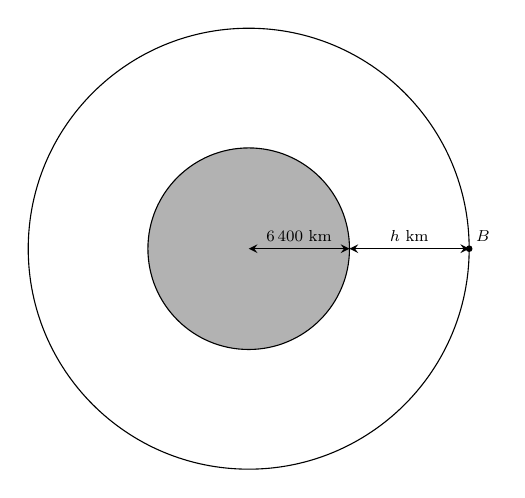
\begin{tikzpicture}[line join = round, line cap=round,>=stealth,font=\footnotesize,transform shape,scale=0.8]
\draw
(0,0) circle(3.5cm)
;
\draw[fill=black!30]
(0,0) circle(1.6cm);
\draw[<->] (0:3.5)--(0:1.6) node[pos=0.5,above]{$h$ km};
\draw[<->] (0:0)--(0:1.6) node[pos=0.5,above]{$6\, 400$ km};
\fill
(3.5,0)circle(1.5pt)node[above right]{$B$};
\end{tikzpicture}}
Trong hệ tọa độ $Oxyz$, gốc tọa độ là tâm trái đất, một vệ tinh nhân tạo tạo quỹ đạo được coi như một đường tròn có bán kính $13440$ km có điểm xuất phát là điểm $B (4032;0;-5376)$ và đây cũng là điểm gần Trái Đất nhất của vệ tinh. Quỹ đạo của vệ tinh này nằm trên mặt phẳng vuông góc với trục tung và có tâm nằm trên đường thẳng $OB$. Coi Trái Đất là hình cầu hoàn hảo có bán kính bằng $6400$ km.
\choiceTF
{Phương trình mặt phẳng chứa quỹ đạo của vệ tinh là $x+z=0$}
{\True Khi xuất phát tại điểm $B$ vệ tinh đang ở độ cao $320$ km so với mặt đất}
{Quỹ đạo của tên lửa là đường tròn có tâm $I(-4032; 0;5120)$}
{Khi Trái Đất quay, điểm cực Nam và cực Bắc của Trái Đất không thay đổi vị trí. Biết rằng điểm cực Nam của Trái Đất có tọa độ là $(0; 3840;5120)$. Khoảng cách gần nhất giữa vệ tinh và điểm cực Nam bằng $10112$ km (làm tròn kết quả đến hàng đơn vị)}
\loigiai{
\begin{itemchoice}
\itemch Quỹ đạo của vệ tinh này nằm trên mặt phẳng vuông góc với trục tung nên một vectơ chỉ phương của
mặt phẳng chứa quỹ đạo của vệ tinh là $(0; 1; 0)$.\\
Khi đó, phương trình mặt phẳng chứa quỹ đạo của vệ tinh có dạng $y+a=0$.\\
Quỹ đạo đi qua $B(4032;0;-5376)$ nên $0+a=0$ hay $a=0$.\\
Vậy phương trình mặt phẳng chứa quỹ đạo của vệ tinh là $y=0$.
\itemch Khoảng cách ngắn nhất từ Trái Đất đến vệ tinh bằng
\[OB-R=\sqrt{4032^{2}+0^{2}+(-5376)^{2}}-6400=320(km).\]
Vậy khi xuất phát tại điểm $B$ vệ tình đang ở độ cao $320$ km so với mặt đất.
\itemch
Quỹ đạo của vệ tinh có tâm nằm trên đường thẳng $OB$ nên $I$ nằm trên đường thẳng $OB$.\\
Mặt khác $IB=R_{qd}=13440=2\cdot OB$ nên $O$ là trung điểm của $IB$.\\
Khi đó
\[\begin{cases}
x_I=2x_O-x_B \\
y_I=2y_O-y_B \\
z_I=2z_O-z_B
\end{cases}
\Leftrightarrow
\begin{cases}
x_I=-4032\\
y_I=0\\
z_I=5376\end{cases}
\Rightarrow I(-4032; 0; 5376).\]
\itemch
Gọi $H$ là hình chiếu của $K$ trên mặt phẳng chứa quỹ đạo $(\alpha)\colon y=0\Rightarrow H(0; 0; 5120)$.\\
Ta có
\begin{itemize}
\item $KH=\mathrm{d}(K, (\alpha))=3840$.
\item $IH=\sqrt{4032^2+(5376-5120)^2}=64\sqrt{3985}$.
\item $NH=IN-IH=13440-64\sqrt{3985}$.
\end{itemize}
Nối $I$ và $H$ cắt vệ tinh tại $N$. Khi đó:
\[KN_{\text{min}}=\sqrt{KH^2+NH^2}=\sqrt{3840^2+(13440-64\sqrt{3985})^2} \approx 10154 \text{ (km)}.\]

\end{itemchoice}
}
\end{ex}

\begin{ex}%[2H5V3-4]%[TEX Đề Moon 2025]%[Võ Nguyên Thạch]
Trong không gian $Oxyz$ (đơn vị trên mỗi trục tính theo mét), một ngọn hải đăng được đặt ở vị trí $I(17;20;45)$. Biết rằng ngọn hải đăng đó được thiết kế với bán kính phủ sáng là $4$ km.
\choiceTF
{\True Phương trình mặt cầu để mô tả ranh giới bên ngoài của vùng phủ sáng trên biển của hải đăng là $(x-17)^2+(y-20)^2+(z-45)^2=16\,000\,000$}
{Nếu người đi biển ở vị trí $M(18;21;50)$ thì không thể nhìn thấy được ánh sáng từ ngọn hải đăng}
{Nếu người đi biển ở vị trí $N(4\,019;21;44)$ thì có thể nhìn thấy được ánh sáng từ ngọn hải đăng}
{\True Nếu hai người đi biển ở vị trí có thể nhìn thấy được ánh sáng từ ngọn hải đăng thì khoảng cách giữa hai người đó không quá $8$ km}
\loigiai{
\begin{itemchoice}
\itemch Ta có $4$ km $=4\,000$ m.\\
Phương trình mặt cầu mô tả ranh giới bên ngoài vùng phủ sáng trên biển của hải đăng là phương trình mặt cầu tâm $I(17;20;45)$, bán kính $4\,000$ m là
\[(x-17)^2+(y-20)^2+(z-45)^2=16\,000\,000.\]
\itemch Ta có $IM=\sqrt{(18-17)^2+(21-20)^2+(50-45)^2}=\sqrt 27<4\,000$.\\
Khi đó, người ở vị trí điểm $M$ có thể nhìn thấy ánh sáng từ ngọn hải đăng.
\itemch Ta có $IN=\sqrt{(4\,019-17)^2+(21-20)^2+(44-45)^2}=\sqrt{16\,016\,006}>4\,000$.\\
Khi đó, người ở vị trí điểm $N$ không thể nhìn thấy ánh sáng từ ngọn hải đăng.
\itemch Vì đường kính của mặt cầu trên bằng $8\,000$ m hay $8$ km nên khoảng cách giữa hai người đi biển ở vị trí có thể nhìn thấy ánh sáng từ ngọn hải đăng không quá $8$ km.
\end{itemchoice}
}
\end{ex}

\begin{ex}%[2H5V3-3]
Trong không gian với tọa độ $Oxyz$, cho mặt cầu $(S)\colon  x^2+y^2+z^2-2x+4y+1=0$ và mặt phẳng $(P)\colon x+y-z-2=0$.
\choiceTF
{Mặt cầu $(S)$ có tâm $I(-1;2;0)$}
{Bán kính của mặt cầu $(S)$ là $R=4$}
{\True Khoảng cách từ tâm $I$ của mặt cầu $(S)$ đến mặt phẳng $(P)$ bằng $\sqrt{3}$}
{\True Mặt phẳng $(P)$ cắt mặt cầu $(S)$ theo giao tuyến là một đường tròn có bán kính $r=1$}
\loigiai{
\begin{itemchoice}
\itemch Mặt cầu $(S)\colon x^2+y^2+z^2-2x+4y+1=0$ có tâm $I(1;-2;0)$.
\itemch Bán kính mặt cầu $(S)\colon  x^2+y^2+z^2-2x+4y+1=0$ là $R=\sqrt{1^2+(-2)^2+0^2-1}=2$.
\itemch Khoảng cách từ tâm $I(1;-2;0)$ của mặt cầu $(S)$ đến mặt phẳng $(P)\colon x+y-z-2=0$ là \[\mathrm{d}(I,(P))=\dfrac{|1+(-2)-0-2|}{\sqrt{1^2+1^2+(-1)^2}}=\sqrt{3}.\]
\itemch Ta thấy $\mathrm{d}(I,(\mathrm{P}))<R$ nên $(P)$ cắt mặt cầu $(S)$ theo giao tuyến là một đường tròn với bán kính
\[R=\sqrt{R^2-\mathrm{d}(I, (P))^2}=\sqrt{2^2-\left(\sqrt{3}\right)^2}=1.\]
\end{itemchoice}
}
\end{ex}

\begin{ex}%[2H5V2-8]%[TEX ĐỀ MOON 2025]%[Huỳnh Thanh Chí]
Trong không gian với hệ tọa độ $Oxyz$, một cabin cáp treo xuất phát từ điểm $A(10;3;0)$ và chuyển động đều theo đường cáp có vectơ chỉ phương $\overrightarrow{u}=(2;-2;1)$ (hướng chuyển động cùng chiều với hướng vectơ $\overrightarrow{u}$ với tốc độ là $4{,}5$ (m/s)) (đơn vị trên mỗi trục là mét). Xét tính đúng sai của các mệnh đề sau
\choiceTF
{\True Phương trình tham số của đường cáp là $\heva{& x=10+2t' \\ & y=3-2t'\\ & z=t'}$ $(t\in\mathbb{R})$}
{\True Giả sử sau thời gian $t$ (s) kể từ khi xuất phát $(t\ge 0)$, cabin đến điểm $M$. Khi đó tọa độ điểm $M$ là $M\left(3t+10;-3t+3;\dfrac{3t}{2}\right)$}
{Cabin dừng ở điểm $B$ có hoành độ $x_B=550$, khi đó quãng đường $AB$ dài $800$ m}
{Đường cáp $AB$ tạo với mặt phẳng $(Oxy)$ một góc $30^\circ$}
\definecolor{ecru}{rgb}{0.76, 0.7, 0.5}
\definecolor{darkolivegreen}{rgb}{0.33, 0.42, 0.18}
\definecolor{deepskyblue}{rgb}{0.0, 0.75, 1.0}
\definecolor{antiquebrass}{rgb}{0.8, 0.58, 0.46}
\definecolor{arsenic}{rgb}{0.23, 0.27, 0.29}
\definecolor{ashgrey}{rgb}{0.7, 0.75, 0.71}\definecolor{alizarin}{rgb}{0.82, 0.1, 0.26}
\begin{center}
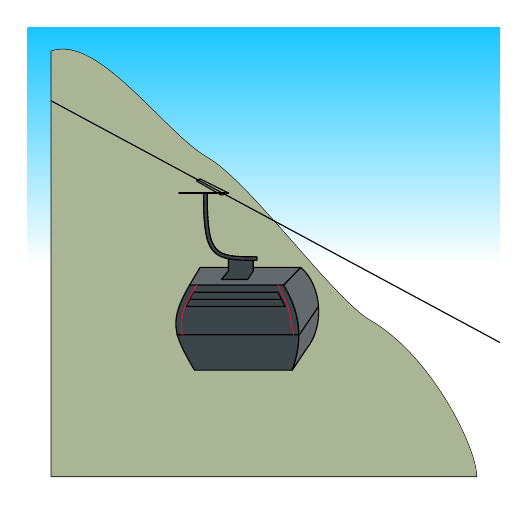
\begin{tikzpicture}[line join=round, line cap=round,scale=1,transform shape]
\clip (-3,-3) rectangle (3,3);
\fill[bottom color=white,top color=deepskyblue!90, middle color=white] (-3,-3) rectangle (3,3);
\tikzset{dat/.pic={
\def\N{
(-3,3)
..controls +(20:.7) and +(150:.7) ..(-.8,1.5)
..controls +(-30:.7) and +(150:.6) ..(1.5,-.8)
..controls +(-30:1) and +(90:.4) ..(3,-3)--(-3,-3)--cycle
;
}
\draw[black]\N;
\fill[darkolivegreen!50] \N;
}}
\tikzset{cap_treo/.pic={
\def\X{
(-.85,1)--(-.8,1)
..controls +(-90:.9) and +(-180:.6) ..(-.1,0.1)--(-.1,.05)
..controls +(-180:.65) and +(-90:.9) ..cycle
(-.15,0.05)--(-.15,-.1)--(-.23,-.22)--(-.6,-.22)--(-.5,-.1)--(-.5,.08)
;
}
%\fill[black] \X;
\draw\X;
\draw(-3,2.3)--(3.5,-1.2);
\draw(-1.2,1)--(-.5,1);
\draw(-.5,1)--(-.9,1.2)--(-.95,1.17)--(-.6,.97)--cycle;
\draw[fill=arsenic!80](-.9,-.05)--(.52,-.05)--(.28,-.3)--(-1.05,-.3)--cycle;
\def\M{
(-.85,1)--(-.8,1)
..controls +(-90:.9) and +(-180:.6) ..(-.1,0.1)--(-.1,.05)
..controls +(-180:.65) and +(-90:.9) ..cycle
(-.15,0.05)--(-.15,-.1)--(-.23,-.22)--(-.6,-.22)--(-.5,-.1)--(-.5,.08)
;
}
\fill[arsenic] \M;
\draw\M;
\def\N{
(-1.05,-.3)
..controls +(-120:.6) and +(120:.6) ..(-.98,-1.5)--(.4,-1.5)
..controls +(70:.6) and +(-60:.3) ..(.28,-.3)--cycle
;
}
\fill[arsenic] \N;
\draw\N;
\def\P{
(.4,-1.5)
..controls +(70:.6) and +(-60:.3) ..(.28,-.3)--(.52,-.05)
..controls +(-40:.4) and +(50:.4) ..(.6,-1.2)--cycle
;
}
\fill[arsenic!80] \P;
\draw\P;
\draw (-1.23,-1)--(.5,-1)--(.77,-.6);
\draw (-1.05,-.5)--(-1,-.4)--(.2,-.4)--(.25,-.5)--cycle
(.25,-.5)--(.3,-.6)--(.3,-.6)--(-1.1,-.6)--(.-1.05,-.5)--cycle
;
\draw[alizarin](.42,-1)..controls +(100:.4) and +(-65:.4) ..(.2,-.3);
\draw[alizarin](-1.15,-1)..controls +(100:.3) and +(-120:.3) ..(-.95,-.3);
}}
\path
(0,0)pic[scale=1]{dat}(0,0)pic[scale=1]{cap_treo};
\end{tikzpicture}
\begin{tikzpicture}[scale=1, font=\footnotesize, line join=round,xscale=.2, line cap=round,>=stealth]
\def\a{1/16}
\def\xmin{-3} \def\xmax{12}
\def\ymin{-3} \def\ymax{3}
\coordinate (O) at (0,0);
\coordinate (E) at (-10,-3);
\coordinate (N) at ($(E)!.7!(O)$);
\coordinate (P) at ($(E)!.2!(O)$);
\coordinate (D) at ($(E)!.3!(O)$);
\coordinate (A) at ($(N)+(3,0)$);
\coordinate (B) at (-14,1);
\coordinate (M) at ($(A)!.7!(B)$);
\draw[->] (\xmin,0)--(\xmax,0) node [above right]{$y$};
\draw[->] (O)--(0,\ymax) node [left]{$z$};
\draw[->] (O)--(E) node [below right]{$x$};
\node at (0,0)[above right]{$O$};
\draw[dashed] (B)--(P)node [right]{$550$} (N)--(A)node [below right]{$A(10;3;0)$}--(3,0);
\draw(B)node [above]{$B$}--(A);
\draw[->,red](O)--(-4,.6)node [above right]{$\overrightarrow{u}$};
\node at (N) [left]{$10$};
\node at (M) [above]{$M$};
\node at (P) [left]{$x_B$};
\draw[fill=black] (3,0) circle (.5pt) node[below]{\footnotesize $3$};
%	\path (-28,0) node[opacity=.5,scale=.5] {\includegraphics{image/h35}};
\clip (\xmin+0.1,\ymin+0.1) rectangle (\xmax-0.1,\ymax-0.1);
\end{tikzpicture}
\end{center}
\loigiai{
\begin{itemchoice}
\itemch Phương trình chính tắc của đường cáp là $\dfrac{x-10}{2}=\dfrac{y-3}{-2}=\dfrac{z}{1}$.\\
Phương trình tham số của đường cáp là $\heva{& x=10+2t' \\ & y=3-2t'\\ & z=t'}$ $(t'\in\mathbb{R})$.
\itemch Do tốc độ chuyển động của cabin là $4{,}5$ m/s nên độ dài $A M$ bằng $4{,}5 t$ m. \\
Vì vậy $\left|\overrightarrow{AM}\right|=4{,}5 t$ $(t \geq 0)$.\\
Do hai vectơ $\overrightarrow{A M}$ và $\overrightarrow{u}$ là cùng phương và cùng hướng nên $\overrightarrow{A M}=k \overrightarrow{u}$ với $k$ là số thực dương nào đó. \\
Suy ra $\left|\overrightarrow{A M}\right|=k|\overrightarrow{u}|=k \cdot \sqrt{2^2+(-2)^2+1}=3 k$. Do đó $3 k=4{,}5 t$. Suy ra $k=\dfrac{3 t}{2}$. \\
Vì thế, ta có $\overrightarrow{A M}=\dfrac{3 t}{2} \overrightarrow{u}=\left(3 t ;-3 t ; \dfrac{3 t}{2}\right)$.\\
Gọi tọa độ của điểm $M$ là $\left(x_M ; y_M ; z_M\right)$.\\
Ta có $\overrightarrow{A M}=\left(x_M-x_A ; y_M-y_A ; z_M-z_A\right)=\left(3 t ;-3 t ; \dfrac{3 t}{2}\right)$.\\
Nên $\heva{&x_M=3 t+x_A \\ &y_M=-3 t+y_A \\ &z_M=\dfrac{3 t}{2}+z_A}\Leftrightarrow\heva{&x_M=3 t+10 \\ &y_M=-3 t+3 \\ &z_M=\dfrac{3 t}{2}.}$
Vậy điểm $M$ có tọạ độ là $\left(3 t+10 ;-3 t+3 ;\dfrac{3 t}{2}\right)$.
\itemch Do $x_B=550$ nên $3 t+10=550$, tức là $t=180$ s. Do đó, ta có điểm $B(550 ;-537 ; 270)$. \\
Vậy $A B=\sqrt{(550-10)^2+(-537-3)^2+(270-0)^2}=\sqrt{656100}=810$ m.
\itemch Đường thẳng $AB$ có vectơ chỉ phương $\overrightarrow{u}=(2 ;-2 ; 1)$ và mặt phẳng $(Oxy)$ có vectơ pháp tuyến $\overrightarrow{k}=(0 ; 0 ; 1)$. Do đó, ta có
\[
\sin (\Delta,(O x y))=|\cos (\overrightarrow{u},\overrightarrow{k})|=\dfrac{\left|\overrightarrow{u} \cdot \overrightarrow{k}\right|}{|\overrightarrow{u}| \cdot|\overrightarrow{k}|}=\dfrac{1}{3 \cdot 1}=\dfrac{1}{3}.\]
Vậy $(\Delta,(O x y)) \approx 19^{\circ}$.
\end{itemchoice}
}
\end{ex}

\begin{ex}%[2H5V2-3]%[TEX ĐỀ MOON 2025]%[Nguyễn Thế Duy]
Trong không gian $Oxyz$, cho mặt phẳng $(P)\colon x-z=0$, đường thẳng $d\colon\heva{& x=1+2t \\ & y=t\\ & z=t}$ và hai điểm $A(1;2;1)$, $B(2;1;4)$. Xét tính đúng sai của các mệnh đề sau
\choiceTF
{\True Điểm $A$ thuộc mặt phẳng $(P)$}
{Hoành độ giao điểm của đường thẳng $d$ và mặt phẳng $(P)$ bằng $1$}
{Biết điểm $I(a;b;c)\in d$, $a>0$ sao cho mặt cầu $(S)$ có tâm $I$ bán kính $R=2\sqrt{2}$ tiếp xúc với $(P)$. Khi đó $a+b+c=9$}
{\True Gọi $\Delta$ là đường thẳng vuông góc với mặt phẳng $(P)$ sao cho khoảng cách từ điểm $A$ đến $\Delta$ bằng $1$. Khi khoảng cách từ $B$ đến $\Delta$ đạt giá trị nhỏ nhất thì $\Delta$ đi qua điểm $M\left(\dfrac{5}{3};\dfrac{5}{3};\dfrac{5}{3}\right)$}
\loigiai{
\begin{itemchoice}
\itemch \textbf{Đúng}.\\
Thay tọa độ điểm $A\left(1; 2; 1\right)$ vào $(P)$ ta được $1 - 1 = 0$.\\
Suy ra $A$ thuộc mặt phẳng $(P)$.
\itemch \textbf{Sai}.\\
Gọi $M$ là giao điểm của đường thẳng $d$ và mặt phẳng $(P)$ suy ra $M\left(1+2t; t; t \right)$ (do $M \in d$).\\
Mà $M \in (P)$ suy ra $1 + 2t - t = 0 \Leftrightarrow t = -1$.\\
Suy ra $M\left(-1; -1; -1 \right)$.\\
Vậy hoành độ giao điểm của đường thẳng $d$ và mặt phẳng $(P)$ bằng $-1$.
\itemch \textbf{Sai}.\\
Do mặt cầu $(S)$ tiếp xúc với $(P)$ nên ta có $\mathrm{d} \left(I, (P) \right) = R = 2\sqrt{2}$.\\
Mà $I \in d$ nên $I\left(1+2t; t; t \right)$.\\
Từ đó ta được $\dfrac{\left|1+2t - t \right|}{\sqrt{1^2 + (-1)^2}} = 2\sqrt{2} \Leftrightarrow \hoac{&t=3\\&t = -5.}$\\
Với $t = -5$ ta được $I\left(-9; -5; -5 \right)$ không thỏa mãn.\\
Với $t = 3$ ta được $I\left(7; 3; 3 \right)$ thỏa mãn.\\
Suy ra $a + b + c = 7 + 3 + 3 = 13$.
\itemch \textbf{Đúng}.\\
Gọi $d_1$ là đường thẳng đi qua $A$ và vuông góc với $P$, ta được $d_1 \colon \heva{&x = 1+t\\&y=2\\&z=1-t.}$\\
Gọi $N$ là hình chiếu vuông góc của $B$ lên $d_1$.\\
Ta có $N \left(1 + t; 2; 1-t \right)$ và $\overrightarrow{BN} = \left(t-1; 1; -t-3 \right)$.\\
Mặt khác $BN \perp d_1$ suy ra $\overrightarrow{BN} \cdot \overrightarrow{AN} = 0 \Leftrightarrow\left(t - 1 \right) \cdot 1 + 1 \cdot 0 + \left(-t - 3 \right) \cdot 1 = 0 \Leftrightarrow t = -1$.\\
Khi đó $N \left(0;2;2 \right)$ và $\overrightarrow{BN} = \left(-2;1;-2 \right)$.\\
Gọi $K$ là hình chiếu vuông góc của $B$ lên $\Delta$. \\
Ta có $BK + KN \geq NB$ suy ra $BK \geq NB - NK$.\\
Dấu \lq\lq $=$\rq\rq \, xảy ra khi $K$, $N$, $B$ thẳng hàng ($K$ nằm giữa $B$, $N$), suy ra $K = \Delta \cap BN$.\\
Ta có $BN \colon \heva{&x = 2 + 2t\\&y=1-t\\&z=4+2t}$ suy ra $K\left(2+2t; 1-t; 4+2t \right)$.\\
Suy ra $\overrightarrow{BK} = \left(2t; -t; 2t\right)$ và $\overrightarrow{KN} = \left(-2-2t;1+t;-2-2t \right)$.\\
Mặt khác $NK = 1$ và $BN = \sqrt{(-2)^2 + 1^2 + (-2)^2} = 3$.\\
Ta có $\overrightarrow{BN} = k\overrightarrow{KN} \Rightarrow \dfrac{2t}{-2-2t} = \dfrac{-t}{1+t} = \dfrac{2t}{-2-2t} = \dfrac{2}{1}$.\\
Từ đó ta được $t = \dfrac{-2}{3}$ suy ra $K\left(\dfrac{2}{3}; \dfrac{5}{3}; \dfrac{8}{3} \right)$.\\
Suy ra $\Delta \colon \heva{&x = \dfrac{2}{3} + t\\&y = \dfrac{5}{3}\\&z = \dfrac{8}{3} - t.}$\\
Dễ thấy với $t = 1$ ta được điểm $\left(\dfrac{5}{3}; \dfrac{5}{3}; \dfrac{5}{3} \right)$ thuộc đường thẳng $\Delta$.
\end{itemchoice}
}
\end{ex}

\begin{ex}%[2H5V1-7]
\immini{Một mái nhà hình tròn được đặt trên 3 cây cột trụ. Các cây cột trụ vuông góc với mặt sàn nhà phẳng và có độ cao lần lượt là $8$m, $9$m, $10$m. Ba chân cột là ba đỉnh của một tam giác đều trên mặt sàn nhà với cạnh dài $8$m. Chọn hệ trục tọa độ như hình vẽ, với $B$ thuộc tia $Ox$, $C$ thuộc tia $Oy$, tia $Oz$ cùng hướng với véc-tơ $\vv{AA'}$; gốc tọa độ $O$ trùng với trung điểm của $AC$ và mỗi đơn vị trên trục có độ dài 1 mét (xem hình vẽ).}{\begin{tikzpicture}[>=stealth,line join=round,line cap=round,font=\footnotesize,scale=1]
\coordinate[label=center:$I$] (I)at(0,2.3);
\begin{scope}[rotate=-18]
\draw[red,fill=blue!30] (I) ellipse (2cm and 1.2cm);
\end{scope}
\coordinate[label=below right:$O$] (O)at(0,0);
\draw[dashed,black]  (-1.4,3.2)coordinate(A')--(1.5,1.4)coordinate(C')--(-0.8,1.8)coordinate(B')--(A') (-1.4,0)coordinate(A)--(1.5,0)coordinate(C) (0,2.33)coordinate(T)--(O)--(-0.8,-0.8)coordinate(B) ($(B')!2/3!(T)$)coordinate(I)--($(B)!2/3!(O)$)coordinate(J);
\draw (-1.8,0)--(A)--(B)--(C);
\draw[->] (1.5,0)--(2,0)node[below]{$y$};
\draw[->] (0,2.33)--(0,4)node[right]{$z$};
\draw[->] (-0.8,-0.8)--(-1.2,-1.2)node[right]{$x$};
\draw[line width=3pt,orange!70!black] (-1.4,0.05)--(-1.4,3.15) (1.5,0.05)--(1.5,1.35) (-0.8,-0.75)--(-0.8,1.75);
\foreach \diem in {T,I,J,O} \fill (\diem)circle(1pt);
\foreach \diem/\vitri in {A/below left,B/left,C/below,A'/above,B'/left,C'/right} \fill (\diem)circle(1pt)node[\vitri]{$\diem$};
\end{tikzpicture}}
\choiceTF
{\True Tọa độ các điểm $A'(0;-4; 10)$, $B'(4\sqrt{3}; 0; 9)$, $C'(0; 4; 8)$}
{\True Phương trình mặt phẳng $\left(A' B' C'\right)$ là $y+4z-36=0$}
{Tọa độ các điểm $A'(0;-4; 10)$, $B'(4\sqrt{3}; 0; 9)$, $C'(0; 4; 8)$}
{\True Phương trình mặt phẳng $\left(A' B' C'\right)$ là $y+4z-36=0$}
\loigiai{
\begin{itemchoice}
\itemch Tọa độ các điểm $A(0;-4; 0)$, $B(4\sqrt{3};0; 0)$, $C(0;4; 0)$, $A'(0;-4; 10)$, $B'(4\sqrt{3}; 0; 9)$, $C'(0; 4; 8)$
\itemch Ta có $\vv{A'B'}=\left(4\sqrt{3};4;-1\right)$; $\vv{A'C'}=\left(-4\sqrt{3};4;-1\right)$.\\
Véc-tơ pháp tuyến của mặt phẳng $(A'B'C')$ là $\vv{n}=\left[\vv{A'B'},\vv{A'C'}\right]=\left(0;8\sqrt{3};32\sqrt{3}\right)=8\sqrt{3}\left(0;1;4\right)$.\\
Phương trình mặt phẳng $(A'B'C')$ là $y+z-36=0$.
\itemch Vec-tơ pháp tuyến của mặt phẳng $(ABC)$ là $\vv{k}=(0;0;1)$.\\
Khi đó $\cos\left((ABC),(A'B'C')\right)=\dfrac{|5|}{\sqrt{4^2+1^2}}=\dfrac{4}{\sqrt{17}}\Rightarrow \left((ABC),(A'B'C')\right)\approx 14^\circ$.\\
Vậy độ dốc của mái khoảng $14^\circ$, mái nhà trên không đạt tiêu chuẩn.
\itemch Gọi $I(a;b;c)$. Suy ra
$\heva{&b+c=36\\&a^2+(b+4)^2+(c-10)^2=\left(a-4\sqrt{3}\right)^2+b^2+(c-9)^2\\&a^2+(b+4)^2+(c-10)^2=a^2+(b-4)^2+(c-8)^2}\Leftrightarrow \heva{&a=\sqrt{5}\\&b=0\\&c=9.}$\\
Vậy $I(\sqrt{5};0;9)$, điểm $I$ cách mặt sàn khoảng $9$ mét.
\end{itemchoice}

}
\end{ex}

\begin{ex}%[2H5V1-7]%[TEX ĐỀ MOON 2025]%[Nguyễn Văn Hiệp]
\immini[thm]
{
Hình minh hoạ sơ đồ một ngôi nhà trong hệ trục tọa độ $Oxyz$, trong đó nền nhà, bốn bức tường và hai mái nhà đều là hình chữ nhật. Xét tính đúng sai của các mệnh đề sau
\choiceTF
{\True Tọa độ của điểm $A$ là $(4;0;0)$}
{Tọa độ của vectơ $\overrightarrow{AH}$ là $(4;5;3)$}
{Tích vô hướng của $\overrightarrow{AH}$ và $\overrightarrow{AF}$ bằng $3$}
{\True Góc dốc của mái nhà, tức là số đo của góc nhị diện có cạnh là đường thẳng $FG$, hai mặt lần lượt là $(FGQP)$ và $(FGHE)$ bằng $26{,}6^{\circ}$ (làm tròn kết quả đến hàng phần mười của độ)}
}
{
\begin{tikzpicture}[font=\footnotesize, line join=round, line cap=round, >=stealth, scale=0.7]
\def\a{3}
\def\b{5}
\def\h{3}
\path (0:0) coordinate (C)
++(0:\a) coordinate (B)
++(-160:\b) coordinate (O)
($(O)+(B)-(C)$) coordinate (A)
($(O)+(90:\h)$) coordinate (E)
($(B)+(90:\h)$) coordinate (G)
($(C)+(90:\h)$) coordinate (H)
($(A)+(90:\h)$) coordinate (F)
($(A)+(0:1)$) coordinate (x)
($(H)+(35:2)$) coordinate (Q)
($(E)+(35:2)$) coordinate (P)
($(E)+(90:1)$) coordinate (z)
($(O)!1.3!(C)$) coordinate (y);
\draw[dashed] (G)--(H)--(C)--(B) (C)--(O);
\draw[] (G)--(Q)--(H)--(E)--(F)--(G)--(B)--(A)--(O)--(E) (F)--(A) (F)--(P)--(E) (P)--(Q);
\draw [->] (A)--(x);
\draw [->] (E)--(z);
\draw [->,dashed] (C)--(y);
\draw [] (Q)node[above]{$Q(2; 5; 4)$} (G)node[right]{$G(4; 5; 3)$} (B)node[right]{$B(4; 5; 0)$} (P)node[right]{$P(2; 0; 4)$} (O)node[below]{$O(0; 0; 0)$} (E)node[left]{$E(0; 0; 3)$} (x)node[below]{$x$} (y)node[above]{$y$} (z)node[left]{$z$};
\foreach \x/\g in {A/-90,C/180,F/0,H/90}
\fill[black] (\x) circle (1pt)
($(\g:4mm)+(\x)$) node {$\x$};
\end{tikzpicture}
}
\loigiai
{
\begin{itemchoice}
\itemch Theo hình vẽ tọa độ điểm $A(4;0;0)$.
\itemch Tọa độ $H(0;5;3)$ suy ra $\overrightarrow{AH} = (-4;5;3)$.
\itemch
Tọa độ $F(4;0;3)$ suy ra $\overrightarrow{AF} = (4;0;3)$ và $\overrightarrow{AH}\cdot \overrightarrow{AF}=-4\cdot 4 + 5\cdot 0 + 3\cdot 3 = -7 \neq 3$.
\itemch
Một vectơ chỉ phương của mặt phẳng $(FGQP)$ là\\ $\overrightarrow{n_1}=\left[\overrightarrow{FP},\overrightarrow{FG}\right]=\left[(-2;0;1),(0;5;0)\right]=(-5;0;10)$.\\
Một vectơ chỉ phương của mặt phẳng $(FGHE)$ là\\ $\overrightarrow{n_2}=\left[\overrightarrow{FG},\overrightarrow{FE}\right]=\left[(0;5;0),(-4;0;0)\right]=(0;0;20)$.\\
Đặt $\theta$ góc nhị diện cạnh $FG$,  hai mặt lần lượt là $(FGQP)$ và $(FGHE)$.\\
Ta có $\cos \theta = \dfrac{\overrightarrow{n}_1 \cdot \overrightarrow{n}_2}{\left|\overrightarrow{n}_1\right|\left|\overrightarrow{n}_2\right|}=\dfrac{2\sqrt{5}}{5}\Rightarrow \theta \approx 26{,}6^\circ$.
\end{itemchoice}
}
\end{ex}

\begin{ex}%[2H5V1-5]%[Tex đề Moon 2025]%[Nguyễn Hồng Thạch]
Trong không gian với hệ tọa độ $Oxyz$, cho hai điểm $A(1;2;-1)$, $B(2;1;0)$ và mặt phẳng $(P)\colon 2x+y-3z+1=0$. Gọi $(Q)$ là mặt phẳng chứa $A$, $B$ và vuông góc với mặt phẳng $(P)$.
\choiceTF
{\True Một vec-tơ pháp tuyến của mặt phẳng $(P)$ là $(2;1;-3)$}
{Một vec-tơ pháp tuyến của mặt phẳng $(Q)$ là $(2;1;-3)$}
{\True Phương trình mặt phẳng $(Q)$ có dạng $ax+by+cz+9=0$. Khi đó $a+b+c=-10$}
{Khoảng cách từ điểm $O$ đến mặt phẳng $(Q)$ bằng $\dfrac{15\sqrt{38}}{38}$}
\loigiai{\begin{itemchoice}
\itemch Dựa vào phương trình mặt phẳng $(P)$ ta thấy $(P)$ có một vec-tơ pháp tuyến là\\ $\overrightarrow{n}_P=(2;1;-3)$.
\itemch Ta có $\overrightarrow{AB}= (1;-1;1)$.\\
Gọi $\overrightarrow{n}_Q$ là vec-tơ pháp tuyến của mặt phẳng $(Q)$.\\
Ta có $\heva{&(P)\perp (Q)\\&(P)\ \text{chứa}\ A,\ B}\Rightarrow \heva{&\overrightarrow{n}_P\cdot \overrightarrow{n}_Q=0\\&\overrightarrow{n}_P\cdot\overrightarrow{AB}=0}\Rightarrow \overrightarrow{n}_Q=\left[\overrightarrow{n}_P,\overrightarrow{AB}\right]=(-2;-5;-3)$.\\
Ta thấy $\overrightarrow{n}_Q=(-2;-5;3)$ khồng cùng phương với $\overrightarrow{n}=(2;1;-3)$ nên $\overrightarrow{n}=(2;1;-3)$ không phải là vec-tơ pháp tuyến của mặt phẳng $(Q)$.
\itemch Mặt phẳng $(Q)$ có vec-tơ pháp tuyến là $\overrightarrow{u}_Q=(-2;-5;-3)$ và đi qua điểm $B(2;1;0)$ nên có phương trình là \[-2\cdot(x-2)-5\cdot(y-1)-3\cdot(z-0)=0\Leftrightarrow -2x-5y-3z+9=0.\]
Suy ra $a=-2$, $b=-5$, $c=-3$.\\
Vậy $a+b+c=-10$.
\itemch Khoảng cách từ  điểm $O$ đến mặt phẳng $(Q)$ là
\[\mathrm{d}(O,(Q))=\dfrac{\left|-2\cdot0-5\cdot0-2\cdot0+9\right|}{\sqrt{(-2)^2+(-5)^2+(-3)^2}}=\dfrac{9\sqrt{38}}{38}.\]
\end{itemchoice}}
\end{ex}

\begin{ex}%[2H2V2-6]
Hình vẽ sau mô tả vị trí của máy bay vào thời điểm $9$h$30$ phút. Biết các đơn vị trên hình tính theo đơn vị km.
\begin{center}
\begin{tikzpicture}[line join = round, line cap=round,>=stealth,font=\footnotesize,scale=1]
\path
(0,0) coordinate (O)
(5,0) coordinate (B)
(-3,-2) coordinate (A)
(0,4) coordinate (C)
($(A)+(B)-(O)$) coordinate (N)
($(N)+(0,4)$) coordinate (M)
;
\draw 	(O)--(B)(O)--(A) (O)--(C);

\foreach \x/\r/\p in{A/180/x,B/90/y,C/90/z}
\draw[->,line width=2pt] (O)--($(O)!1.2!(\x)$)node[scale=1.5,shift={(\r:3mm)}]{$\p$};
;

%\draw pic[draw,angle radius=7mm] {angle = M--O--C};
\draw (A) node[shift={(150:4mm)}]{$150$};
\draw (B) node[shift={(90:4mm)}]{$300$};
\draw (C) node[shift={(180:4mm)}]{$9$};
\draw (B) node[shift={(-70:4mm)}]{(Đông)};
\draw (A) node[shift={(-30:4mm)}]{(Nam)};


\draw[dashed] (O)--(N)--(B) (A)--(N)--(M)--(C);
\draw[->,line width=2pt] (O)--(M);


\draw (M) node[yshift=.4cm]{	\begin{tikzpicture}[line join = round, line cap=round,>=stealth,font=\footnotesize,scale=0.15]

\draw[cyan,line width=3pt]
(0,0)--(0.2,-0.5)coordinate (A)--(5,-1.2)coordinate (O)
(10,0)--(9.8,-0.5)coordinate (A')--(5,-1.2)
(5,-0.8) circle(0.7cm)
($(A)!0.6!(O)+(0,-0.3)$) circle(0.3cm)
($(A)!0.6!(O)+(0,-0.3)$) circle(0.2cm)
($(A')!0.6!(O)+(0,-0.3)$) circle(0.3cm)
($(A')!0.6!(O)+(0,-0.3)$) circle(0.2cm)
(7,0)--(5,-0.3) -- (3,0)
(5,-0.3)--(5,1.2)
;
\fill[cyan] (5,-0.8) circle(0.7cm);

\fill[black,xshift=-0.05cm] (4.5,-0.7) rectangle (4.6,-0.5)
(4.7,-0.7) rectangle (4.8,-0.5)
(4.9,-0.7) rectangle (5,-0.5)
(5.1,-0.7) rectangle (5.2,-0.5)
(5.3,-0.7) rectangle (5.4,-0.5)
(5.5,-0.7) rectangle (5.6,-0.5)
;


\draw[line width=2pt]
($(A')!0.75!(O)$)--($(A')!0.75!(O)+(0,-0.65)$)
($(A')!0.75!(O)+(0,-0.65)$)--++(0:0.2)
($(A')!0.75!(O)+(0,-0.65)$)--++(180:0.2)--++(-90:0.1)
($(A')!0.75!(O)+(0,-0.65)$)--++(180:0.2)--++(90:0.1)
($(A')!0.75!(O)+(0,-0.65)$)--++(0:0.2)--++(-90:0.1)
($(A')!0.75!(O)+(0,-0.65)$)--++(0:0.2)--++(90:0.1)
($(A)!0.75!(O)$)--($(A)!0.75!(O)+(0,-0.65)$)
($(A)!0.75!(O)+(0,-0.65)$)--++(0:0.2)
($(A)!0.75!(O)+(0,-0.65)$)--++(180:0.2)--++(-90:0.1)
($(A)!0.75!(O)+(0,-0.65)$)--++(180:0.2)--++(90:0.1)
($(A)!0.75!(O)+(0,-0.65)$)--++(0:0.2)--++(-90:0.1)
($(A)!0.75!(O)+(0,-0.65)$)--++(0:0.2)--++(90:0.1)
;
\end{tikzpicture}	}
;
\end{tikzpicture}
\end{center}
\choiceTF
{\True Máy bay đang ở độ cao $9$ km}
{ Tọa độ của máy bay lúc này là $(300; 150; 9)$}
{\True Phi công để máy bay ở chế độ tự động với vận tốc theo hướng đông là $750$ km/h, độ cao không đổi. Biết rằng gió thổi theo hướng đông với vận tốc $10$ m/s. Giả sử vận tốc và hướng gió không đổi thì lúc $10$h$30$ phút máy bay ở tọa độ là $(150; 1086; 9)$}
{Sau khi bay đến vị trí lúc $10$h$30$ thì máy bay bay ngược lại (hướng tây) với vận tốc $800$ km/h với độ cao không đổi, biết lúc đó trời lặng gió thì lúc $11$h máy bay ở tọa độ $(686; 150; 9)$}
\loigiai{
\begin{itemchoice}
\itemch  {\bf Đúng.}\\
Dựa vào hình vẽ ta thấy máy bay đang ở độ cao $9$ km.
\itemch  {\bf Sai.}\\
Máy bay đang ở tọa độ $(150; 300; 9)$.
\itemch  {\bf Đúng.}\\
Vận tốc gió $10$ m/s $= 36$ km/h.\\
Máy bay bay tự động trong khoảng thời gian từ $9$h$30$ đến $10$h$30$ với quãng đường $750$ km.\\
Quãng đường thực tế máy bay bay được là $750+36=786$ km.\\
Do đó tọa độ máy bay là $(150; 1\,086; 9)$.
\itemch  {\bf Sai.}\\
Quãng đường máy bay bay được trong khoảng thời gian từ $10$h$30$ đến $11$h là \[800\cdot \dfrac{1}{2}=400\,\, \text{km}.\]
Do đó tọa độ máy bay là $(150; 868; 9)$.
\end{itemchoice}
}
\end{ex}

\begin{ex}%[50 Đề minh họa tốt nghiệp 2025 - Đề 13]%[Lê Hữu Kiệt - Lê Quân]%[2H2V2-6]
Một chiếc điện thoại được đặt trên một giá đỡ có ba chân với điểm đặt $S(0;0;20)$ và các điểm chạm mặt đất của ba chân lần lượt là $A(0;-6;0)$, $B(3\sqrt{3};3;0)$, $C(-3\sqrt{3};3;0)$ (đơn vị cm). Cho biết điện thoại có trọng lượng là $2$ N và ba lực tác dụng lên giá đỡ được phân bố như hình vẽ là ba lực $\overrightarrow{F}_1$, $\overrightarrow{F}_2$, $\overrightarrow{F}_3$ có độ lớn bằng nhau và đo bằng đơn vị N.
\begin{center}
\tdplotsetmaincoords{75}{115}
\begin{tikzpicture}[font=\footnotesize, line join=round, line cap=round, >=stealth, scale=0.4, tdplot_main_coords]
\pgfmathsetmacro\bancanba{3*sqrt(3)}
\draw[->] (-7,0,0) -- (9,0,0) node[anchor=north east] {$x$};
\draw[->] (0,-7,0) -- (0,7,0) node[anchor=north west] {$y$};
\draw[->] (0,0,10.8) -- (0,0,12) node[anchor=south] {$z$};
\path
(0,0,0) coordinate (O)
(0,-6,0) coordinate (A)
(\bancanba,3,0) coordinate (B)
(-\bancanba,3,0) coordinate (C)
(0,0,9) coordinate (S);
\draw[dashed] (0,0,0) circle [radius=6] (A)--(B)--(C)--cycle (S)--(O);
\draw (S)--(A) (S)--(B) (S)--(C);
\foreach \x [count=\i from 1] in {A,B,C}{
\path ($(S)!1/3!(\x)$) coordinate (f\i);
\draw[->] (S)--(f\i)node[right=-1mm]{$\overrightarrow{F}_\i$};
}
\draw[rounded corners=1] (0,-2,8.9) rectangle (0,2,11);
\fill (0,-2,9.2) rectangle (0,-1.8,10.2);
\foreach \x/\g in {C/above right, A/above left, B/below, S/above right, O/below}{
\fill (\x) circle (3.3pt)node[\g]{$\x$};
}
\end{tikzpicture}
\end{center}
\choiceTF
{\True $\overrightarrow{SA}=(0;-6;-20)$}
{$\overrightarrow{F}_1+\overrightarrow{F}_2+\overrightarrow{F}_3=\overrightarrow{F}(0;0;2)$}
{$\left|\overrightarrow{F}_1\right|=\dfrac{1}{20}\left|\overrightarrow{SA}\right|$}
{\True Biết tọa độ của lực $\overrightarrow{F}_1=(a;b;c)$, khi đó $T=2a+5b+6c=-5$}
\loigiai{
\begin{itemchoice}
\itemch Ta có $\overrightarrow{SA}=(0;-6;-20)$.
\itemch Ta có $\overrightarrow{F}_1+\overrightarrow{F}_2+\overrightarrow{F}_3=\overrightarrow{F}$, do điện thoại có trọng lượng là $2$ N nên $\left|\overrightarrow{F}\right|=2$.\\
Lại có $\left|\overrightarrow{SO}\right|=20$, $\overrightarrow{F}$ và $\overrightarrow{SO}=(0;0;-20)$ cùng hướng nên $\overrightarrow{F}=\dfrac{1}{10}\overrightarrow{SO}$.\\
Suy ra $\overrightarrow{F}=(0;0;-2)$.
\itemch Do ba lực $\overrightarrow{F}_1$, $\overrightarrow{F}_2$, $\overrightarrow{F}_3$ có độ lớn bằng nhau nên với cùng số $k$, ta có $\overrightarrow{F}_1=k\overrightarrow{SA}$, $\overrightarrow{F}_2=k\overrightarrow{SB}$ và $\overrightarrow{F}_3=k\overrightarrow{SC}$.\\
Ta có $\overrightarrow{SB}=(3\sqrt3;3;-20)$, $\overrightarrow{SC}=(-3\sqrt3;3;-20)$. Khi đó
\[ \overrightarrow{F}_1+\overrightarrow{F}_2+\overrightarrow{F}_3=\overrightarrow{F} \Leftrightarrow \heva{& k\cdot0+k\cdot3\sqrt3+k\cdot(-3\sqrt3) =0 \\& k\cdot(-6)+k\cdot3+k\cdot3=0 \\& k\cdot(-20)+k\cdot(-20)+k\cdot(-20)=-2} \Leftrightarrow k=\dfrac{1}{30}. \]
Suy ra $\overrightarrow{F}_1=\dfrac{1}{30}\overrightarrow{SA}$.\\
Vậy $\left|\overrightarrow{F}_1\right|=\dfrac{1}{30}\left|\overrightarrow{SA}\right|$.
\itemch Ta có $\overrightarrow{F}_1=\dfrac{1}{30}\overrightarrow{SA}$ suy ra $\overrightarrow{F}_1=\left(0;-\dfrac{1}{5};-\dfrac{2}{3}\right)$. Do đó $a=0$, $b=-\dfrac{1}{5}$, $c=-\dfrac{2}{3}$.\\
Vậy $T=2a+5b+6c=-5$.
\end{itemchoice}
}
\end{ex}

\begin{ex}%[2H2V2-6]
Một máy bay đang di chuyển về phía sân bay. Tại thời điểm hiện tại, vị trí của máy bay là $B(150;150;5\,000)$ (trong đó $5\,000$ m là độ cao của máy bay so với mặt đất). Máy bay đang di chuyển thẳng tới sân bay $C(0;0;0)$ với vận tốc $700$ km/h. Xét tính đúng sai của các mệnh đề sau:
\choiceTF
{\True Phương trình tham số của đường thẳng mà máy bay di chuyển theo là $\heva{& x=150-150t \\ & y=150-150t\\ & z=5\,000-5\,000t}$}
{Khoảng cách từ vị trí hiện tại của máy bay $B$ đến sân bay $C$ xấp xỉ bằng $3\,905{,}6$ km}
{Với vận tốc trung bình của máy bay là $700$ km/h, thời gian để máy bay hạ cánh là khoảng $5{,}5$ giờ}
{Nếu hệ thống kiểm soát không lưu yêu cầu liên lạc với máy bay khi nó còn cách sân bay $40$ km thì khi máy bay ở vị trí $(6;6;200)$, nó còn cách sân bay là $40$ km}
\loigiai{
\begin{itemchoice}
\itemch
Véc-tơ chỉ phương của đường thẳng $BC$ là $\overrightarrow{BC}=(-150;-150;-5\,000)$.\\
Phương trình tham số của đường thẳng đi qua $B(150;150;5\,000)$ và nhận $\overrightarrow{BC}$ làm véc-tơ chỉ phương  là
$\heva{& x=150-150t \\ & y=150-150t \\ & z=5\,000-5\,000t}$.
\itemch
Khoảng cách từ $B$ đến $C$ là độ dài đoạn thẳng \allowdisplaybreaks
\begin{eqnarray*}
BC=\left|\overrightarrow{BC}\right|=\sqrt{(-150)^2+(-150)^2+(-5\,000)^2}\approx 5\,004{,}5\,\, (\text{m})=5{,}0\,045\,\, (\text{km}).
\end{eqnarray*}
\itemch
Vận tốc $v=700$ km/h. Quãng đường $d=BC \approx 5{,}0\,045$ km.\\
Thời gian để máy bay hạ cánh (đi hết quãng đường $BC$) là $\dfrac{5{,}0\,045}{700} \approx 0{,}00\,715=$ (giờ).\\
\itemch
Xét vị trí $\mathrm{P}\left(6;6;200\right)$. \\	Khoảng cách từ $\mathrm{P}\left(6;6;200\right)$ đến sân bay $C(0;0;0)$ là \\
$PC=\sqrt{(6-0)^2+(6-0)^2+(200-0)^2}\approx200{,}18\,\, (\text{m})= 0{,}200$ km.
\end{itemchoice}
}
\end{ex}

\begin{ex}%[2H2V2-2]%[TEX Đề Moon 2025]%[Vũ Hồng Toàn]
Trong không gian $Oxyz$, cho tam giác $ABC$ có $A(-1;2;4)$, $B(3;0;-2)$, $C(1;3;7)$. Gọi $D$ là chân đường phân giác trong của góc $A$. Xét tính đúng sai của các mệnh đề sau
\choiceTF
{\True Độ dài cạnh $AB$ là $2\sqrt{14}$}
{Trọng tâm của tam giác $ABC$ là điểm $G(1;2;3)$}
{\True Tích vô hướng $\overrightarrow{AB}\cdot \overrightarrow{AC}$ bằng $-12$}
{\True Độ dài vectơ $\overrightarrow{OD}$ bằng $\dfrac{\sqrt{205}}{3}$}
\loigiai{
\begin{itemchoice}
\itemch Ta có $AB = \sqrt{4^2 + (-2)^2 + (-6)^2} = \sqrt{16 + 4 + 36} = 2\sqrt{14}$.
\itemch Ta có $G\left(\dfrac{-1+3+1}{3};\dfrac{2+0+3}{3};\dfrac{4-2+7}{3}\right)\Rightarrow G\left(1;\dfrac{5}{3};3\right)$.
\itemch $\overrightarrow{AB}=(4;-2;-6)$ và $\overrightarrow{AC}=(2;1;3)$.\\
Vậy $\overrightarrow{AB}\cdot \overrightarrow{AC}=4\cdot 2-2\cdot 1-6\cdot 3=-12$.
\itemch
\immini{
Ta có $AB = 2\sqrt{14}$ và $AC = \sqrt{14}$. Gọi $D(x;y;z)$\\
Khi đó $\dfrac{BD}{DC}=\dfrac{AB}{AC}=\dfrac{2\sqrt{14}}{\sqrt{14}}=2$.\\
Suy ra $\overrightarrow{DB}=-2\overrightarrow{DC}$
}
{
\begin{tikzpicture}[declare function={gocc=35;a=4;b=3;}]
\path (0,0) coordinate (B)++(a,0) coordinate (C) ++(180-gocc:b) coordinate (A)
($(A)!1cm!(B)$) coordinate (AB)
($(A)!1cm!(C)$) coordinate (AC)
($(AB)!0.5!(AC)$) coordinate (At)
(intersection of A--At and B--C) coordinate (D);
\foreach\x/\y/\z in {B/A/D}{
\path pic[draw,angle radius=7pt]{ angle=\x--\y--\z};}
\foreach\x/\y/\z in {D/A/C}{
\path pic[draw,angle radius=9pt]{ angle=\x--\y--\z};}
\draw (A)--(B)--(C)--cycle --(D);
\foreach \x/\goc in {A/90,B/180,C/-90,D/-90}{
\draw[fill] (\x) circle (1pt) node[shift={(\goc:7pt)},font=\small]{$\x$};
}
\end{tikzpicture}
}
$\Rightarrow\heva{&3-x=-2(1-x)\\&-y=-2(3-y)\\&-2-x=-2(7-x)}\Rightarrow\heva{&x=\dfrac{5}{3}\\&y=2\\&z=4.}$\\
Vậy $OD=\sqrt{\left(\dfrac{5}{3}\right)^2+2^2+4^2}=\dfrac{\sqrt{205}}{3}$.
\end{itemchoice}
}
\end{ex}

\begin{ex}%[2D6V2-4]%[TEX ĐỀ MOON 2025]%[Nguyễn Cường]
Lớp 12A có $30$ học sinh, trong đó có $17$ bạn nữ còn lại là nam. Có $3$ bạn tên Hiền, trong đó có $1$ bạn nữ và $2$ bạn nam. Thầy giáo gọi ngẫu nhiên $1$ bạn lên bảng. Các mệnh đề sau đúng hay sai?
\choiceTF
{\True Xác suất để có tên Hiền là $\dfrac{1}{10}$}
{Xác suất để có tên Hiền, nhưng với điều kiện bạn đó nữ là $\dfrac{3}{17}$}
{\True Xác suất để có tên Hiền, nhưng với điều kiện bạn đó nam là $\dfrac{2}{13}$}
{Nếu thầy giáo gọi $1$ bạn có tên là Hiền lên bảng thì xác xuất để bạn đó là bạn nữ là $\dfrac{3}{17}$}
\loigiai{
\begin{itemchoice}
\itemch Gọi $A$ là biến cố \lq\lq bạn Hiền lên bảng\rq\rq.\\
Suy ra $n(A)=3$.\\
Xác suất $\mathrm{P}(A)=\dfrac{n(A)}{n(\Omega)}=\dfrac{3}{30}=\dfrac{1}{10}$.
\itemch Gọi $B$ là biến cố \lq\lq bạn nữ lên bảng\rq\rq, suy ra $\mathrm{P}(B)=\dfrac{17}{30}$.\\
$AB$ là biến cố \lq\lq bạn nữ tên Hiền lên bảng\rq\rq, suy ra $\mathrm{P}(AB)=\dfrac{1}{30}$.\\
Khi đó, xác suất để có tên Hiền, nhưng với điều kiện bạn đó nữ là $\mathrm{P}(A\mid B)=\dfrac{\mathrm{P}(AB)}{\mathrm{P}(B)}=\dfrac{1}{17}$.
\itemch Xác suất để có tên Hiền, nhưng với điều kiện bạn đó nam là $\mathrm{P}(A\mid \overline{B})=\dfrac{2}{13}$.
\itemch Áp dụng công thức Bayes ta có
\allowdisplaybreaks
\begin{eqnarray*}
\mathrm{P}(B\mid A)&=&\dfrac{\mathrm{P}(A\mid B)\cdot \mathrm{P}(B)}{\mathrm{P}(A)}\\
&=&\dfrac{\dfrac{1}{17}\cdot\dfrac{1}{30}}{\dfrac{1}{10}}\\
&=&\dfrac{1}{51}.
\end{eqnarray*}
\end{itemchoice}
}
\end{ex}

\begin{ex} %[2D6V2-3]
Nobita và Shizuka chuẩn bị đi tham quan hòn đảo Honshu trong hai ngày thứ Bảy và Chủ nhật tuần này. Ở hòn đảo Honshu này, mỗi ngày chi có nắng hoặc mưa, nếu một ngày là nắng thì khả năng xảy ra mưa ở ngày ngày tiếp theo là $20\%$, còn nếu một ngày là mưa thì khả năng ngày hôm sau vẫn mưa là $30\%$. Theo dự báo thời tiết, xác suất trời sẽ nắng vào thứ Bảy tuần này là $0{,}7$. Gọi $A$ là biến cố \lq\lq Ngày thứ Bảy tuần này trời nắng\rq\rq\, và $B$ là biến cố \lq\lq Ngày Chủ nhật tuần này trời mưa\rq\rq.
\choiceTF
{\True $P(A)=0{,}7$}
{Xác suất có điều kiện $P(\overline{B} \mid A)=0{,}77$}
{Xác suất ngày chủ nhật tuần này trời nắng là $80\%$}
{Bạn mèo máy Doraemon có thể đến được tương lai nhưng lại chỉ đến hòn đảo vào ngày Chủ nhật và báo cho Nobita biết rằng Chủ nhật tuần này trời mưa, khi đó xác suất ngày thứ 7 trời nắng là $62\%$ (làm tròn đến hàng đơn vị theo đơn vị phần trăm)}
\loigiai{
\begin{center}
\begin{tikzpicture}
\def\gocm{20}
\def\gocn{10}
\def\r{4}
\tikzset{s/.style={outer sep=0.5 mm,draw=magenta,rectangle,minimum width=2.75cm,rounded corners=1mm}}
\path(0,0)node(O){}++(\gocm:\r)node[s](A1){Nắng (A)}++(\gocn:\r)node[s](A2){Mưa (B)};
\path(A1)++({-\gocn}:\r)node[s](a2){Nắng $(\overline{B})$};
\path(O)++(-\gocm:\r)node[s](B1){Mưa $(\overline{A})$}++(\gocn:\r)node[s](B2){Mưa (B)};
\path(B1)++({-\gocn}:\r)node[s](b2){Nắng $(\overline{B})$};
\foreach \x/\y in {
O/A1,A1/A2,
O/B1,B1/B2,
A1/a2,
B1/b2}
\draw[-stealth](\x.east)--(\y.west);
\path(O)--(A1.west)node[pos=0.5,above,sloped]{$\mbox{0{,}7}$}(O)--(B1.west)node[pos=0.5,below]{$\mbox{0{,}3}$}(B1.east)--(B2.west)node[pos=0.5,above]{$\mbox{0{,}3}$}(A1.east)--(A2.west)node[pos=0.5,above]{$\mbox{0{,}2}$}
(A1.east)--(a2.west)node[pos=0.5,below,sloped]{$\mbox{0{,}8}$}
(B1.east)--(b2.west)node[pos=0.5,below,sloped]{$\mbox{0{,}7}$};
%%Node dòng trên
\path(A2)++(0,1)node{\textbf{Chủ nhật}}++(180:4)node{\textbf{Thứ bảy}};
\end{tikzpicture}
\end{center}
Ta có sơ đồ hình cây như hình vẽ.\\
Ta có $A$ là biến cố \lq\lq Ngày thứ Bảy tuần này trời nắng\rq\rq\, và $B$ là biến cố \lq\lq Ngày Chủ nhật tuần này trời mưa\lq\lq.
\begin{itemchoice}
\itemch Theo giả thiết ta có $P(A)=0{,}7$.
\itemch Ta có $ \mathrm{P}(\overline{B} \mid A)=\dfrac{ \mathrm{P}(\overline{B} \cap A)}{ \mathrm{P}(A)}=\dfrac{ \mathrm{P}(\overline{B})\cdot  \mathrm{P}(A \mid \overline{B})}{ \mathrm{P}(A)}=0{,}8$.
\itemch Theo công thức xác suất toàn phần ta có
\begin{eqnarray*}
\mathrm{P}(\overline{B}) &=& \mathrm{P}(A) \cdot \mathrm{P}(\overline{B}|A) +\mathrm{P}\left(\overline{A}\right) \cdot  \mathrm{P}\left(\overline{B}|\overline{A}\right)\\
&=& 0{,}7 \cdot 0{,}8+ 0{,}3\cdot 0{,}7= 0{,}77.
\end{eqnarray*}
\itemch Ta có $ \mathrm{P}(A\mid B)=\dfrac{ \mathrm{P}(A \cap B)}{ \mathrm{P}(B)}=\dfrac{ \mathrm{P}(A)\cdot  \mathrm{P}(B \mid A)}{ \mathrm{P}(B)}$.\\
$ \mathrm{P}(B)=\mathrm{P}(A \cap B)+\mathrm{P}(\overline{A} \cap B)=\mathrm{P}(A)\cdot\mathrm{P}(B\mid A)+\mathrm{P}(\overline{A})\cdot\mathrm{P}(B\mid \overline{A})=0{,}23$.\\
Do đó $ \mathrm{P}(A\mid B)=\dfrac{ \mathrm{P}(A \cap B)}{ \mathrm{P}(B)}=\dfrac{ \mathrm{P}(A)\cdot  \mathrm{P}(B \mid A)}{ \mathrm{P}(B)}=\dfrac{0{,}7 \cdot 0{,}2}{0{,}23}=0{,}6087\approx 61\%$.
\end{itemchoice}
}
\end{ex}

\begin{ex}%[2D6V2-2]
Chuồng I có $3$ con gà trống và $7$ con gà mái, chuồng II có $4$ con gà trống và $5$ con gà mái. Có $1$ con gà từ chuồng I sang chuồng II. Sau đó, có $1$ con gà từ chuồng II chạy ra ngoài.\\
Gọi $A$ là biến cố có $1$ con gà mái từ chuồng I sang chuồng II.\\
Gọi $B$ là biến cố một con gà từ chuồng II chạy ra ngoài là gà trống.
\choiceTF
{\True $\mathrm{P}(A)=0{,}7$}
{$\mathrm{P}(B\mid A)=0{,}5$}
{\True Xác suất để con gà từ chuồng II chạy ra ngoài là gà trống là $43\%$}
{\True Biết con gà từ chuồng II chạy ra ngoài là gà mái, xác suất để con gà từ chuồng I sang chuồng II là gà trống là $\dfrac{5}{19}$}
\loigiai{
\begin{itemchoice}
\itemch Ta có $\mathrm{P}(A)=\dfrac{\mathrm{C}_7^1}{\mathrm{C}_{10}^1}=0{,}7$.\\
Gọi $A$ là biến cố có $1$ con gà mái từ chuồng I sang chuồng II.\\
Suy ra $\mathrm{P}(A)=\dfrac{\mathrm{C}_3^1}{\mathrm{C}_{10}^1}=0{,}3$.
\itemch Ta có $\mathrm{P}(B\mid A)=\dfrac{\mathrm{C}_4^1}{\mathrm{C}_{10}^1}=0{,}4$.
\itemch Ta có $P\left(B \mid \overline{A}\right)=\dfrac{\mathrm{C}_5^1}{\mathrm{C}_{10}^1}=0{,}5$.\\
Ta có sơ đồ cây sau
\begin{center}
\begin{tikzpicture}[declare function={dai=2.5;cao=0.65;},>=stealth,font=\scriptsize]
\tikzset{nhan/.style={minimum size=19pt,font=\small,inner sep=0pt}}
\path (0,0) node[nhan] (G){\text{Gốc}}
(dai,{1.5*cao}) node[nhan] (B) {$A$}
(dai,{-1.5*cao}) node[nhan] (nB) {$\overline{A}$}
({2*dai},{3*cao}) node[nhan] (BA) {$B$}
({2*dai},{cao}) node[nhan] (BnA) {$\overline{B}$}
({2*dai},{-cao}) node[nhan] (nBA) {$B$}
({2*dai},{-3*cao}) node[nhan] (nBnA) {$\overline{B}$};

%Phần mũi tên
\draw[->] (G.0)--(B.200) node[sloped,pos=0.5,above]{$0{,}7$};
\draw[->] (G.0)--(nB.160) node[sloped,pos=0.5,below]{$0{,}3$};
\draw[->] (B.10)--(BA.190) node[sloped,pos=0.5,above]{$0{,}4$};
\draw[->] (B.10)--(BnA.170) ;
\draw[->] (nB.-10)--(nBA.190) node[sloped,pos=0.5,above]{$0{,}5$};
\draw[->] (nB.-10)--(nBnA.170) ;
\end{tikzpicture}
\end{center}
Áp dụng công thức xác suất toàn phần, ta có \[\mathrm{P}(B)=\mathrm{P}(A)\cdot \mathrm{P}(B\mid A)+\mathrm{P}\left(\overline{A}\right)\cdot \mathrm{P}\left(B\mid\overline{A}\right)=0{,}7 \cdot 0{,}4+0{,}3 \cdot 0{,}5=0{,}43=43\%.\]
\itemch
Ta có $\mathrm{P}\left(\overline{B}\right)=1-\mathrm{P}(B)=0{,}57$.\\
Suy ra \[\mathrm{P}\left(\overline{A} \mid\overline{B}\right)=\dfrac{\mathrm{P}\left(\overline{A B}\right)}{\mathrm{P}\left(\overline{B}\right)}=\dfrac{\dfrac{3}{10} \cdot\dfrac{ \mathrm{C}_5^1}{ \mathrm{C}_{10}^1}}{0,57}=\dfrac{5}{19}.\]
\end{itemchoice}
}
\end{ex}

\begin{ex}%[2D6V1-4]
Một công ty đấu thầu hai dự án. Khả năng thắng thầu của các dự án lần lượt là $0{,}4$ và $0{,}5$. Khả năng thắng thầu cả hai dự án là $0{,}3$. Gọi $A$, $B$ lần lượt là biến cố thắng thầu dự án $1$ và dự án $2$. Xét tính đúng sai của các mệnh đề sau
\choiceTF
{Hai biến cố $A$ và $B$ độc lập}
{\True Biết công ty thắng thầu dự án $1$, thì xác suất công ty thắng thầu dự án $2$ là $0{,}75$}
{Biết công ty không thắng thầu dự án $1$, thì xác suất công ty thắng thầu dự án $2$ là $\dfrac{2}{3}$}
{\True Xác suất công ty thắng thầu đúng $1$ dự án là $0{,}3$}
\loigiai{
\begin{itemchoice}
\itemch
Ta có $P(A)\cdot B(B)=0{,}4\cdot 0{,}5=0{,}2\ne 0{,}3=P(AB)$.
\itemch
Xác suất để công ty thắng thầu dự án $2$ khi đã biết thắng thầu dự án $1$ là $P(B|A)$.\\
Ta có $P(B| A)=\dfrac{P(AB)}{P(A)}=\dfrac{0{,}3}{0{,}4}=0{,}75$.
\itemch
Xác suất để công ty thắng thầu dự án $2$ khi đã biết điều kiện không thắng thầu dự án $1$ là $P(B\setminus \overline{A})=\dfrac{P(\overline{A}B)}{P(\overline{A})}$.\\
Vì hai biến cố $\overline{A}B$ và $AB$ xung khắc và $\overline{A}B\cap AB=B$ nên theo tính chất của xác suất ta có
$P(\overline{A}B)=P(B)-P(AB)$. Suy ra
\begin{eqnarray*}
P(B|\overline{A})&=&\dfrac{P(\overline{A}B)}{P(\overline{A})}=\dfrac{P(B)-P(AB)}{1-P(A)}\\
&=&\dfrac{0{,}5-0{,}3}{1-0{,}4}=\dfrac{1}{3}.
\end{eqnarray*}
\itemch
Xác suất để công ty thắng thầu đúng $1$ dự án là $P(A\overline{B})+P(\overline{A}B)$.\\
Vì hai biến cố $\overline{A}B$ và $AB$ xung khắc và $\overline{A}B\cap AB=B$ nên theo tính chất của xác suất ta có
\[P(\overline{A}B)=P(B)-P(AB)\quad(1).\]
Vì hai biến cố $A\overline{B}$ và $AB$ xung khắc và $A\overline{B}\cap AB=A$ nên theo tính chất của xác suất ta có \[P(A\overline{B})=P(A)-P(AB)\quad(2).\]
Từ $(1)$ và $(2)$ ta có
\begin{eqnarray*}
P(A\overline{B})+P(\overline{A}B)&=&P(A)-P(AB)+P(B)-P(AB)\\
&=& P(A)+P(B)-2P(AB)\\
&=& 0{,}4+0{,}5-2\cdot 0{,}3=0{,}3.
\end{eqnarray*}
\end{itemchoice}
}
\end{ex}

\begin{ex}%[2D6V1-2]
Một công ty truyền thông đấu thầu $2$ dự án.Khả năng thắng thầu của dự án $1$ là $0{,}5$ và dự án $2$ là $0{,}6$.Khả năng thắng thầu của cả $2$ dự án là $0{,}4$.Gọi $A$,$B$ lần lượt là biến cố thắng thầu dự án $1$ và dự án $2$.Xét tính đúng sai của các mệnh đề sau
\choiceTF
{\True Xác suất $\mathrm{P}\left(\overline{A}\right)=0{,}5$ và $\mathrm{P}\left(\overline{B}\right)=0{,}4$}
{\True Xác suất công ty thắng thầu đúng $1$ dự án là $0{,}3$}
{Biết công ty thắng thầu dự án $1$,xác suất công ty thắng thầu dự án $2$ là $0{,}4$}
{Biết công ty không thắng thầu dự án $1$,xác suất công ty thắng thầu dự án $2$ là $0{,}8$}
\loigiai{
Ta có $\mathrm{P}(A)=0{,}5$,$\mathrm{P}(B)=0{,}6$,$\mathrm{P}\left(A \cap B\right)=0{,}4$.
\begin{itemchoice}
\itemch
Xác suất không thắng thầu dự án $1$ là $\mathrm{P}\left(\overline{A}\right)=1-\mathrm{P}(A)=1-0{,}5=0{,}5$.\\
Xác suất không thắng thầu dự án $2$ là $\mathrm{P}\left(\overline{B}\right)=1-\mathrm{P}(B)=1-0{,}6=0{,}4$.
\itemch
Biến cố công ty thắng thầu đúng $1$ dự án là $\left(A \cap \overline{B}\right) \cup \left(\overline{A} \cap B\right)$.\\
Xác suất thắng dự án $1$ mà không thắng dự án $2$ là \allowdisplaybreaks
\begin{eqnarray*}
\mathrm{P}\left(A \cap \overline{B}\right)=\mathrm{P}(A)-\mathrm{P}\left(A \cap B\right)=0{,}5-0{,}4=0{,}1.
\end{eqnarray*}
Xác suất không thắng dự án 1 mà thắng dự án $2$ là \allowdisplaybreaks
\begin{eqnarray*}
\mathrm{P}\left(\overline{A} \cap B\right)=\mathrm{P}(B)-\mathrm{P}\left(A \cap B\right)=0{,}6-0{,}4=0{,}2.
\end{eqnarray*}
Vì hai biến cố $(A \cap \overline{B})$ và $(\overline{A} \cap B)$ xung khắc nên xác suất thắng đúng $1$ dự án là  \allowdisplaybreaks
\begin{eqnarray*}
\mathrm{P}\left((A \cap \overline{B}\right) \cup (\overline{A} \cap B))=\mathrm{P}\left(A \cap \overline{B}\right)+\mathrm{P}\left(\overline{A} \cap B\right)=0{,}1+0{,}2=0{,}3.
\end{eqnarray*}

\itemch
Xác suất công ty thắng thầu dự án $2$ biết đã thắng thầu dự án $1$ là xác suất có điều kiện
\allowdisplaybreaks
\begin{eqnarray*}
\mathrm{P}\left(B \mid A\right)=\dfrac{\mathrm{P}\left(A \cap B\right)}{\mathrm{P}(A)}=\dfrac{0{,}4}{0{,}5}=\dfrac{4}{5}=0{,}8.
\end{eqnarray*}
\itemch
Xác suất công ty thắng thầu dự án $2$ biết đã không thắng thầu dự án $1$ là xác suất có điều kiện \allowdisplaybreaks
\begin{eqnarray*}
\mathrm{P}\left(B \mid \overline{A}\right)=\dfrac{\mathrm{P}\left(\overline{A} \cap B\right)}{\mathrm{P}\left(\overline{A}\right)}=\dfrac{0{,}2}{0{,}5}=\dfrac{2}{5}=0{,}4.
\end{eqnarray*}
\end{itemchoice}
}
\end{ex}

\begin{ex}%[2D4V3-5]%[Tex đề Moon 2025]%[Nguyễn Hồng Thạch]
Cho hai hình trụ có cùng bán kính bằng $3$ được đặt lồng vào nhau sao cho trục của hai hình trụ vuông góc với nhau và cắt nhau tại $O$ (hình 1). Gọi $(H)$ là phần giao của hai hình trụ (hình 2). Chọn trục $Ox$ vuông góc với hai trục của hình trụ như hình vẽ. Cắt khối $(H)$ bởi mặt phẳng vuông góc với trục $Ox$ tại điểm có hoành độ $x$ $(-3\le x\le 3)$, ta được thiết diện có diện tích là $S(x)$.
\begin{center}
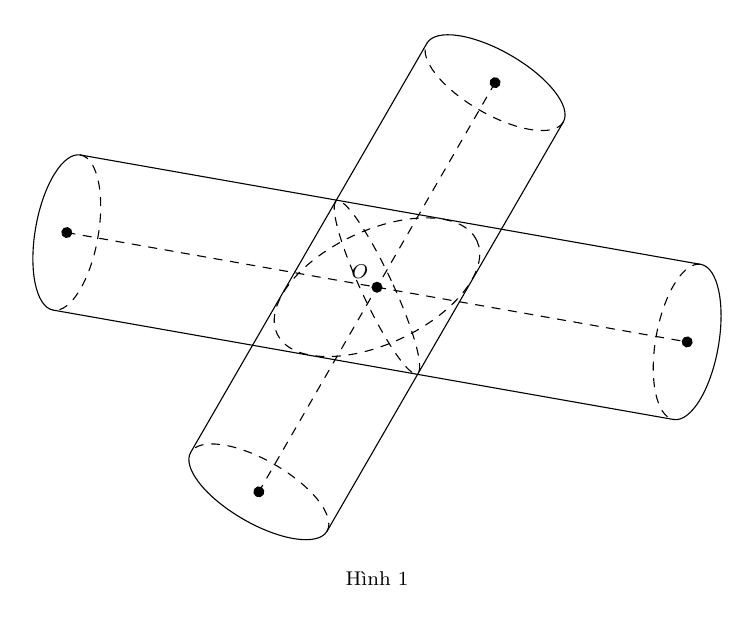
\begin{tikzpicture}[scale=1,>=stealth, font=\footnotesize, line join=round, line cap=round]
\fill (0,0)node[above left]{$O$}circle(2pt);
\begin{scope}[rotate=-10]
\fill (4,0)circle(2pt);
\fill (-4,0)circle(2pt);
\draw[dashed] (-4,0)--(4,0);
\draw (-4,1) arc(90:270:0.4 cm and 1 cm);
\draw[dashed] (-4,1) arc(90:-90:0.4 cm and 1 cm);
\draw[dashed] (4,1) arc(90:270:0.4 cm and 1 cm);
\draw (4,1) arc(90:-90:0.4 cm and 1 cm);
\draw (-4,1)--(4,1) (-4,-1)--(4,-1);
\end{scope}
\begin{scope}[rotate=-30]
\fill (0,-3)circle(2pt);
\fill (0,3)circle(2pt);
\draw[dashed] (0,3)--(0,-3);
\draw (1,3) arc(0:180:1 cm and 0.4 cm);
\draw[dashed] (1,3) arc(360:180:1 cm and 0.4 cm);
\draw[dashed] (1,-3) arc(0:180:1 cm and 0.4 cm);
\draw (1,-3) arc(360:180:1 cm and 0.4 cm);
\draw (1,-3)--(1,3) (-1,-3)--(-1,3);
\end{scope}
\begin{scope}[rotate=25]
\draw[dashed] (0,0) ellipse (1.4 cm and 0.72 cm);
\draw[dashed] (0,0) ellipse (0.2 cm and 1.21 cm);
\end{scope}
\draw (0,-3.5)node[below]{Hình 1};
% \begin{scope}[xshift=8cm,scale=2]
% \draw[->] (0,-1)--(0,1.5)node[left]{$x$};
% \fill (0,0)node[left]{$O$}circle(1pt);
% \draw[rotate=25] (-15:1.4 cm and 0.72 cm) arc(-15:195:1.4 cm and 0.72 cm);
% \draw[rotate=25,dashed] (-15:1.4 cm and 0.72 cm) arc(-15:-165:1.4 cm and 0.72 cm);
% \draw[rotate=25] (0,-1.21) arc(-90:90:0.2 cm and 1.21 cm);
% \draw[dashed,rotate=25] (0,1.21) arc(90:270:0.2 cm and 1.21 cm);
% \draw[rotate=25] (0,1.21)--(32:1.4 cm and 0.72 cm) (0,1.21)--(148:1.4 cm and 0.72 cm);
% \draw[rotate=25] (-15:0.2 cm and 1.21 cm)--(22:1.4 cm and 0.72 cm) (-15:0.2 cm and 1.21 cm)--(158:1.4 cm and 0.72 cm);
% \draw[rotate=25] (-165:1.4 cm and 0.72 cm) parabola bend (0,-1.21) (-15:1.4 cm and 0.72 cm);
% \draw (0,-1.75)node[below]{Hình 2};
% \end{scope}
\end{tikzpicture}
\end{center}
Xét tính đúng sai của các mệnh đề sau
\choiceTF
{Hình khối $(H)$ là một khối tròn xoay}
{Công thức tính thể tích khối $(H)$ là $V=\pi\displaystyle\int\limits_{-3}^{3} S^2(x) \mathrm{\,d}x$}
{Diện tích $S(x)$ được xác định bởi công thức $S(x)=2\left(9-x^2\right)$}
{\True Thể tích của khối $(H)$ bằng $144$ (đvtt)}
\loigiai{
\begin{itemchoice}
\itemch  Khối $(H)$ là phần giao của hai hình trụ, không phải khối tròn xoay.
\itemch  Thể tích là $V = \displaystyle \int_{-3}^{3} S(x)\mathrm{\,d}x$.
\itemch  Thiết diện vuông góc trục $Ox$ là hình vuông cạnh $2\sqrt{9 - x^2}$ nên diện tích là
\[
S(x) = \left(2\sqrt{9 - x^2}\right)^2 = 4(9 - x^2).
\]
\itemch  Ta có
\[
S(x) = 4(9 - x^2) \Rightarrow V = \displaystyle\int_{-3}^{3} 4(9 - x^2)\mathrm{\,d}x = 4\displaystyle\int_{-3}^{3} (9 - x^2)\mathrm{\,d}x.
\]
Do hàm chẵn nên
\[
V = 4 \cdot 2\displaystyle\int_{0}^{3} (9 - x^2)\mathrm{\,d}x = 8 \left[ 9x - \dfrac{x^3}{3} \right]\Big|_0^3 = 8(27 - 9) = 144.
\]
\end{itemchoice}
}
\end{ex}

\begin{ex}%[2D4V3-5]
Một bình nhiên liệu trên cánh máy bay phản lực được mô hình hóa bằng cách quay hình phẳng giới hạn bởi đồ thị $y=f(x)=\dfrac{3}{5}x^2\sqrt{2-ax}$ $(a\in\mathbb{R})$ và trục $Ox$ quanh trục hoành, trong đó $x$ và $y$ được đo bằng mét (như hình vẽ). Biết rằng chiếc máy bay đó có $4$ bình chứa nhiên liệu như nhau và được đổ đầy trước khi bay. Giả sử tốc độ tiêu hao nhiên liệu trên máy bay được mô phỏng bằng hàm số $h'(t)=-3t^2+120t+2000$ lít/giờ ($t$ tính theo giờ, $0\le t\le 6$).
\begin{center}
\begin{tikzpicture}[scale=1,>=stealth, font=\footnotesize, line join=round, line cap=round]
\def\xmin{-1} \def\xmax{3}
\def\ymin{-1} \def\ymax{2}
\draw[->] (\xmin,0)--(\xmax,0) node [below]{$x$};
\draw[->] (0,\ymin)--(0,\ymax) node [left]{$y$};
\node at (0,0) [below left]{$O$};
\draw (1.5,1.3)node[]{$y=\dfrac{3}{5}x^2\sqrt{2-ax}$};
\clip (\xmin+0.1,\ymin+0.1) rectangle (\xmax-0.5,\ymax-0.1);
\draw[smooth,samples=300,domain=0:2] plot(\x,{3/5*(\x)^2*(2-\x)});
\end{tikzpicture}
\end{center}

\choiceTF
{Giá trị $a=2$}
{Thể tích của nhiên liệu (lít) trên mỗi cánh máy bay được xác định bởi công thức $V=\pi\displaystyle\int\limits_{0}^{2} f^2(x) \mathrm{\,d}x$}
{\True Máy bay đó có thể chứa tối đa $9650$ lít nhiên liệu (làm tròn đến hàng đơn vị)}
{\True Máy bay đó tiêu hao hết $90\%$ năng lượng sau $3{,}91$ giờ (làm tròn đến hàng phần trăm)}
\loigiai{
\begin{itemchoice}
\itemch Ta có \begin{eqnarray*}
y(2)=0 & \Leftrightarrow& \dfrac{3}{5} \cdot 2^2 \sqrt{2-2a}=0 \\
& \Leftrightarrow& \sqrt{2-2a}=0 \Leftrightarrow 2-2 a=0 \\
& \Leftrightarrow& a=1 .
\end{eqnarray*}
\itemch Thể tích của nhiên liệu trên mỗi bình nhiên liệu được xác định bởi công thức $V=\pi \displaystyle\int\limits_0^2 f^2(x) \mathrm{d} x ~\left(\mathrm{m}^3\right)$.
\itemch Thể tích của nhiên liệu trên mỗi bình nhiêu liệu bằng
\begin{eqnarray*}
V_{1 b}&=&\pi \displaystyle\int\limits_0^2 f^2(x) \mathrm{d} x \\
& =&\pi \displaystyle\int\limits_0^2\left(\dfrac{3}{5} x^2 \sqrt{2-x}\right)^2 \mathrm{d} x \\
& =&\dfrac{96 \pi}{125}\left(\mathrm{m}^3\right) .
\end{eqnarray*}
Suy ra thể tích của 4 bình nhiên liệu bằng
\[V_{4 b}=4 \cdot \dfrac{96 \pi}{125}=\dfrac{384 \pi}{125}\left(\mathrm{m}^3\right)=3072 \pi~(\mathrm{l}) \approx 9651~(\mathrm{l}) .\]
\itemch Tốc độ tiêu hao nhiên liệu trên máy bay được mô phỏng bởi hàm số\\
$h'(t)=-3 t^2+120 t+2000$ (lít/giờ).\\
$V_{t t}=0{,}9 \cdot V_{4 b}=0{,}9 \cdot 3072 \pi=\dfrac{13824}{5} \pi$ (l) .\\
Gọi $m$ là thời gian máy bay đó sẽ tiêu hao hết $90$ năng lượng, khi đó
\begin{eqnarray*}
\displaystyle\int\limits_0^m h'(t) \mathrm{d}t=\dfrac{13824 \pi}{5}
& \Leftrightarrow& \displaystyle\int\limits_0^m\left(-3 t^2+120 t+2000\right) \mathrm{d}t=\dfrac{13824 \pi}{5} \\
& \Leftrightarrow&-t^3+60 t^2+\left.2000 t\right|_0 ^m=\dfrac{13824 \pi}{5} \\
& \Leftrightarrow&-m^3+60 m^2+2000 m=\dfrac{13824 \pi}{5} \\
& \Leftrightarrow&\hoac{
&m \approx 82{,}87 \\
&m \approx 3{,}91 \\
&m \approx-26{,}78
} \\
& \Leftrightarrow& m \approx 3{,}91 .
\end{eqnarray*}
Vậy máy bay đó sẽ tiêu hao hết $90$ năng lượng sau $3{,}91$ giờ bay.
\end{itemchoice}
}
\end{ex}

\begin{ex}%[2D4V3-3]%[TEX ĐỀ MOON 2025]%[Lê Hữu Kiệt]
Trong mặt phẳng tọa độ $Oxy$, cho hàm số $f(x)=x^2-x-6$ có đồ thị $(C)$.
\choiceTF
{\True Thể tích của vật thể tròn xoay được sinh ra khi hình phẳng giới hạn bởi đồ thị $(C)$ và trục hoành quay quanh $Ox$ là $V=\pi\displaystyle\int\limits_{-2}^{3} \left(x^2-x-6\right)^2 \mathrm{d}x$}
{Diện tích hình phẳng giới hạn bởi đồ thị $(C)$ và trục hoành là $S=\displaystyle\int\limits_{-2}^{3} \left(x^2-x-6\right) \mathrm{d}x$}
{Giả sử một vật $M$ chuyển động dọc theo một đường thẳng sao cho vận tốc của nó tại thời điểm $x$ (giây) là $f(x)=x^2-x-6$ (m/s). Khi đó độ dịch chuyển của vật $M$ trong khoảng thời gian $x\in[1;4]$ là $\dfrac{9}{2}$}
{\True Tổng quãng đường của vật $M$ ở trên đi được trong khoảng thời gian $x\in[1;4]$ là $\dfrac{61}{6}$ (m)}
\loigiai{
\begin{itemchoice}
\itemch Ta có $f(x)=0\Leftrightarrow x^2-x-6=0 \Leftrightarrow \hoac{&x=3\\&x=-2.}$\\
Khi đó thể tích của vật thể tròn xoay được sinh ra khi hình phẳng giới hạn bởi đồ thị $(C)$ và trục hoành quay quanh $Ox$ là $V=\pi\displaystyle\int\limits_{-2}^{3} \left(x^2-x-6\right)^2 \mathrm{d}x$.
\itemch Diện tích hình phẳng giới hạn bởi đồ thị $(C)$ và trục hoành là
\[S=\displaystyle\int\limits_{-2}^{3} \left|x^2-x-6\right|\mathrm{d}x=\displaystyle\int\limits_{-2}^{3}\left(-x^2+x+6\right)\mathrm{d}x.\]
\itemch Với $x=1$ ta có $f(1)=-6$, ta được điểm $A(1;-6)$.\\
Với $x=4$ ta có $f(4)=6$, ta được điểm $B(4;6)$.\\
Khi đó độ dịch chuyển của chất điểm $M$ trong khoảng thời gian $x\in[1;4]$ là
\[AB=\sqrt{(4-1)^2+(6+6)^2}=3\sqrt{17}.\]
\itemch Tổng quãng đường của một vật $M$ trong khoảng thời gian $x\in[1;4]$ là
\[\int\limits_1^4 \left|x^2-x-6\right|\mathrm{d}x=-\int\limits_1^3\left(x^2-x-6\right)\mathrm{d}x+\int\limits_3^4\left(x^2-x-6\right)\mathrm{d}x=\dfrac{61}{6}.\]
\end{itemchoice}
}
\end{ex}

\begin{ex}%[2D4V3-2]%[TEX Đề Moon 2025]%[Vũ Hồng Toàn]
Cho hàm số $y=f(x)$ có $f'(x)=2\cos^2\dfrac{x}{2}+3$, $\forall x\in \mathbb{R}$. Các mệnh đề sau đúng hay \textbf{sai}?
\choiceTF
{\True Hàm số $y=f(x)$ có dạng $f(x)=\sin x+4x+C$ với $C$ là hằng số}
{\True $\displaystyle\int\limits_{0}^{\tfrac{\pi}{2}} f(x)\mathrm{\,d}x=F\left(\dfrac{\pi}{2}\right)-F(0)$ với $F(x)$ là một nguyên hàm của $f(x)$}
{\True Nếu $f(0)=4$ thì $f\left(\dfrac{\pi}{2}\right)=2\pi+5$}
{Diện tích hình phẳng giới hạn bởi đồ thị của hai hàm số $y=f'(x)$; $y=6$ và hai đường thẳng $x=0$, $x=\dfrac{\pi}{2}$ có dạng $S=a+b\pi$ thì $a+2b=-1$}
\loigiai{
\begin{itemchoice}
\itemch $\forall x\in \mathbb{R}$ ta có $f'(x)=2\cos^2\dfrac{x}{2}+3=\left(2\cos^2\dfrac{x}{2}-1\right)+4=\cos x+4$.\\
Do đó $f(x)=\sin x+4x+C$.
\itemch Với $F(x)$ là một nguyên hàm của $f(x)$ khi đó $\displaystyle\int\limits_{0}^{\tfrac{\pi}{2}} f(x)\mathrm{\,d}x=F(x)\bigg |_0^{\tfrac{\pi}{2}}=F\left(\dfrac{\pi}{2}\right)-F(0)$.
\itemch Do $f(x)=\sin x+4x+C$. Nếu $f(0)=4\Rightarrow C=4$ thì $f(x)=\sin x+4x+4$.\\
Vậy $f\left(\dfrac{\pi}{2}\right)=\sin\dfrac{\pi}{2}+4\cdot \dfrac{\pi}{2}+4=2\pi+5$.
\itemch Ta có\\ $S=\displaystyle\int\limits_{0}^{\tfrac{\pi}{2}} \big|\cos x+4-6\big|\mathrm{\,d}x=\displaystyle\int\limits_{0}^{\tfrac{\pi}{2}} \big(2-\cos x\big)\mathrm{\,d}x=\left(2x-\sin x\right)\bigg|_0^{\tfrac{\pi}{2}}=\pi -1$.\\
Suy ra $a=-1$ và $b=1$. Vậy $a+2b=-1+2\cdot 1=1$.
\end{itemchoice}
}
\end{ex}

\begin{ex}%[2D4V2-6]
Hệ thống lọc nước bể bơi vô cùng quan trọng để nguồn nước được làm sạch thường xuyên và giữ vệ sinh cho người bơi. Trong quá trình vận hành lọc nước thì lượng nước trong bể sẽ thay đổi theo thời gian. Lượng nước trong bể giảm nếu hệ thống đang xả nước bẩn ra khỏi bể và tăng nếu hệ thống đang cấp thêm nước sạch cho bể. Biết rằng $1$ gallon gần bằng $3{,}785$ lít, dung tích của bể là $1000$ gallon và thời điểm $6$ giờ sáng bể chứa $250$ gallon nước. Hàm số $f(t)$ liên tục trên đoạn [$0;12$] biểu thị cho tốc độ thay đổi lượng nước trong bể theo thời gian $t$ giờ, từ thời điểm $6$ giờ sáng đến $6$ giờ chiều được cho bởi hàm số $
f (t)=\heva{&100 t,&&0 \le t \le 3\\
&-200 t+a,&&3 \le t \le 6\\
&100 t-900, && \le t \le 12
},(a \in\mathbb{R})$.\\
Với mốc thời gian $t=0$ tại thời điểm $6$ giờ sáng.
\choiceTF
{ Tại thời điểm $9$ giờ sáng, nước trong bể đang tăng với tốc độ $600$ gallon/giờ}
{\True Giá trị của $a=900$}
{Tốc độ thay đổi Iượng nước trong bể bằng $0$ vào lúc $11$ giờ trưa và $15$ giờ chiều}
{\True Lượng nước trong bể lớn nhất trong khoảng thời gian từ $9$ giờ sáng đến $18$ giờ chiều là $700$ gallon nước}
\loigiai{
\begin{itemchoice}
\itemch Do $t=0$ tại thời điểm $6$ giờ sáng nên tại thời điểm $9$ giờ sáng thì $t=3$.\\
Ta có $f(3)=100\cdot 3=300$ gallon/giờ.
\itemch Với $t=3$, $100t=-200t+a\Leftrightarrow-600+a=300\Leftrightarrow a=900$.
\itemch Tại $11$ giờ trưa (tương đương $t=5$), tốc độ thay đổi lượng nước trong bể là $f(5)=-200\cdot 5+900=-100$ gallon/giờ.\\
Tại $15$ giờ chiều (tương đương $t=9$), tốc độ thay đổi lượng nước trong bể là $f(9)=100\cdot 9-900=0$ gallon/giờ.
\itemch Từ $9$ giờ sáng đến $18$ giờ chiều tức là $3\le t\le 12$.\\
Từ $3\le t\le 9$, lượng nước đang giảm về $0$.\\
Lượng nước trong bể bắt đầu tăng trở lại từ $9\le t\le 12$.\\
Lượng nước trong bể từ $15$ giờ chiều đến $18$ giờ chiều là
\[250+\displaystyle\int\limits_9^{12}(100 t-900)\mathrm{\, d}t=700 .\]
\end{itemchoice}
}
\end{ex}

\begin{ex}%[2D4V2-6]%[TEX ĐỀ MOON 2025]%[Nguyễn Văn Hiệp]
Một vật được ném lên từ độ cao $300$ m với vận tốc cho bởi công thức $v(t)=-9{,}81t+29{,}43$ (m/s). Gọi $h(t)$ (m) là độ cao của vât so với mặt đất tại thời điểm $t$ (s) tính từ lúc bắt đầu ném vật. Xét tính đúng sai của các mệnh đề sau
\choiceTF
{\True Vận tốc của vật triệt tiêu tại thời điểm $t=3$ giây}
{Hàm số $h(t)=-4{,}985t^2+29{,}43t$}
{\True Vật đạt độ cao lớn nhất là $344$ (m) (làm tròn đến hàng đơn vị)}
{\True Sau $11$ giây tính từ lúc ném thì vật đó chạm đất (làm tròn đến hàng đơn vị)}
\loigiai
{
\begin{itemchoice}
\itemch  $v(t)=-9{,}81t+29{,}43=0\Rightarrow t=3$ m/s
\itemch  $h(t) = 300+\displaystyle \int\limits_{0}^t\left(-9{,}81z+29{,}43\right)\mathrm{\,d}z=-4,905t^2 + 29,43t + 300$.
\itemch Vật đạt độ cao lớn nhất khi $t =-\dfrac{b}{2a}=-\dfrac{29{,}43}{2\cdot \left(-4{,}905\right)} = 3$ s; $h_{\text{max}}=h(3) \approx 344$ m.
\itemch Vật chạm đất khi $h(t)=0\Leftrightarrow -4,905t^2 + 29,43t + 300 = 0$ giải được $t \approx 11$ s.
\end{itemchoice}
}
\end{ex}

\begin{ex}%[2D4V2-6]
Một ô tô đang chạy với tốc độ $108$ km/h thì người lái xe bất ngờ phát hiện chướng ngại vật trên đường. Người lái xe phản ứng một giây sau đó bằng cách đạp phanh khẩn cấp. Kể từ thời điểm này, ô tô chuyển động chậm dần đều với tốc độ $v(t)=-10t+30$ (m/s), trong đó $t$ là thời gian tính bằng giây kể từ lúc đạp phanh. Gọi $s(t)$ là quãng đường xe ô tô đi được trong $t$ (s) kể từ lúc đạp phanh. Xét tính đúng sai của các mệnh đề sau:
\choiceTF
{\True Công thức biểu diễn hàm số $s(t)=-5t^2+30t$ (m)}
{Thời gian kể từ lúc đạp phanh đến khi xe ô tô dừng hẳn là $6$ giây}
{\True Sau $3$ giây kể từ lúc đạp phanh,quãng đường xe ô tô di chuyển được là $45$ (m)}
{Quãng đường xe ô tô đã di chuyển kể từ lúc người lái xe phát hiện chướng ngại vật trên đường đến khi xe ô tô dừng hẳn là $120$ (m)}
\loigiai{
Đổi đơn vị: $108$ km/h $= \dfrac{108 \cdot 1000}{3600}$ m/s $= 30$ m/s.\\
Vận tốc của xe tại thời điểm bắt đầu đạp phanh ($t=0$) là $v(0) = -10(0) + 30 = 30$ (m/s).
\begin{itemchoice}
\itemch
Quãng đường $s(t)$ xe đi được kể từ lúc đạp phanh ($t=0$) là nguyên hàm của vận tốc $v(t)$.\\
$s(t) = \displaystyle\int v(t) \, \mathrm{d}t = \displaystyle\int (-10t+30) \, \mathrm{d}t = -10 \dfrac{t^2}{2} + 30t + C = -5t^2 + 30t + C$.\\
Tại $t=0$ (lúc bắt đầu đạp phanh), quãng đường đi được kể từ lúc đó là $s(0)=0$. \\
Thay $t=0$ vào biểu thức $s(t)$, ta có $s(0) = -5(0)^2 + 30(0) + C = 0 \Rightarrow C = 0$. \\
Vậy $s(t) = -5t^2 + 30t$ (m).
\itemch
Xe dừng hẳn khi vận tốc $v(t) = 0$. \\
$-10t + 30 = 0 \Leftrightarrow 10t = 30 \Leftrightarrow t = 3$ (s). \\
Vậy thời gian kể từ lúc đạp phanh đến khi xe dừng hẳn là $3$ giây.
\itemch
Quãng đường xe ô tô di chuyển được sau $3$ giây kể từ lúc đạp phanh là $s(3)$.\\
$s(3) = -5(3)^2 + 30(3) = -5 \cdot 9 + 90 = -45 + 90 = 45$ (m).
\itemch
Quá trình di chuyển gồm $2$ giai đoạn:
\begin{itemize}
\item Giai đoạn 1: Phản ứng (1 giây). Xe chạy với tốc độ không đổi $30$ m/s.
Quãng đường $s_1 = 30 \cdot 1 = 30$ (m).
\item Giai đoạn 2: Đạp phanh đến khi dừng hẳn (từ $t=0$ đến $t=3$ giây).
Quãng đường $s_2 = s(3) = 45$ (m) (tính ở câu trên).
\end{itemize}
Tổng quãng đường từ lúc phát hiện chướng ngại vật đến khi dừng hẳn là: \\
$S = s_1 + s_2 = 30 + 45 = 75$ (m).
\end{itemchoice}
}
\end{ex}

\begin{ex}%[2D4V1-6]%[TEX ĐỀ MOON 2025]%[Huỳnh Thanh Chí]
Một ô tô bắt đầu chuyển động thẳng nhanh dần đều với tốc độ $v(t)=5t$ (m/s); trong đó $t$ là thời gian tính bằng giây kể từ khi ô tô bắt đầu chuyển động. Đi được $6$ (s) người lái xe phát hiện chướng ngại vật và phanh gấp, ô tô tiếp tục chuyển động chậm dần đều với gia tốc $a=-5$ (m/s$^2$). Xét tính đúng sai của các mệnh đề sau
\choiceTF
{\True Tốc độ của ô tô tại thời điểm $10$ (s) tính từ lúc xuất phát là $10$ (m/s)}
{Quãng đường ô tô chuyển động được trong $6$ giây đầu tiên là $80$ m}
{\True Quãng đường $s$ (đơn vị: mét) mà ô tô chuyển động được kể từ lúc bắt đầu đạp phanh đến khi dừng lại được tính theo công thức $s=\displaystyle\int\limits_{0}^{6} \left(30-5t\right) \mathrm{\,d}t$}
{Quãng đường ô tô chuyển động được kể từ lúc bắt đầu chuyển động cho đến khi dừng lại là $170$ m}
\loigiai{
Gọi $v_1(t)$ là tốc độ chuyển động chậm dần đều của ô tô khi đạp phanh.\\
Ta có $v_1(t)=\int a\mathrm{\,d}t=\int -5\mathrm{\,d}t=-5t+C$.\\
Ta có vận tốc lúc ô tô đạp phanh là $v_1(0)=v(6)=5\cdot 6=30$ m/s.\\
Suy ra tốc độ chuyển động chậm dần đều khi đạp phanh là $v_1(t)=30-5t$ (m/s).
\begin{itemchoice}
\itemch Khi ô tô di chuyển được $6$ (s) thì bắt đầu đạp phanh và tiếp tục chuyển động với tốc độ $v_1(t)$ (m/s).\\
Do đó, tốc độ của ô tô tại thời điểm $10$ (s) tính từ lúc xuất phát bằng tốc độ ô tô chuyển động tại thời điểm $4$ (s) với tốc độ $v_1(t)$ (m/s).\\
Vậy $v_1(4)=30-5\cdot 4=10$ m/s.
\itemch Quãng đường ô tô chuyển động được trong $6$ giây đầu tiên là $S_1=\displaystyle\int\limits_{0}^{6} v(t)\mathrm{\,d}t=90$ m.
\itemch Quãng đường $s$ (đơn vị: mét) mà ô tô chuyển động được kể từ lúc bắt đầu đạp phanh đến khi dừng lại được tính theo công thức $s=\displaystyle\int\limits_{0}^{6} \left(30-5t\right) \mathrm{\,d}t$.
\itemch Khi ô tô dừng lại thì ta có phương trình $v_1(t)=0\Leftrightarrow t=6$ (s).\\
Quãng đường ô tô chuyển động được kể từ lúc bắt đầu chuyển động cho đến khi dừng lại là $S=S_1+S_2=30+\int\limits_{0}^{6} v_1(t)\mathrm{\,d}t=90+90=180$ m.
\end{itemchoice}
}
\end{ex}

\begin{ex}%[2D4V1-6]
Một viên muối hình cầu có đường kính $8$ cm đang tan trong nước với tốc độ giảm thể tích tại bất kỳ thời điểm nào tỷ lệ thuận với diện tích bề mặt quả cầu tại thời điểm đó. Sau $30$ giây thì viên muối tan được một nửa. Gọi $V(t)$ và $r(t)$ lần lượt là thể tích và bán kính của viên muối sau $t$ phút. Xét tính đúng sai của các mệnh đề sau
\choiceTF
{\True Thể tích của viên muối sau $t$ phút được xác định bởi công thức $V(t)=\dfrac{4}{3}\pi r^3(t)$}
{\True Tốc độ giảm thể tích của viên muối là $V'(t)=k\pi r^2(t)$ với $k$ là hằng số}
{Giá trị của $k=-4$}
{Sau $45$ giây thì thể tích của viên muối còn lại là $4{,}2$ cm$^3$ (làm tròn đến hàng phần mười)}
\loigiai{
\begin{itemchoice}
\itemch
Thể tích của viên muối sau thời gian $t$ phút là $V(t)=\dfrac{4}{3}\pi r^3(t)$.
\itemch
Ta có $r(0)=4$ cm.\\
$V(0)=\dfrac{4}{3}\pi r^3(0)=\dfrac{4}{3}\pi\cdot4^3=\dfrac{256\pi}{3}$.
\itemch
Ta có $V(t)=\dfrac{4}{3} \pi r^3(t) \Rightarrow V^{\prime}(t)=\dfrac{4}{3} \pi \cdot 3 r^2(t) \cdot r^{\prime}(t)=4 \pi \cdot r^2(t) \cdot r^{\prime}(t)$.\\
Ta lại có $V'(t)=k\pi\cdot r^2(t)$. Suy ra $r'(t)=\dfrac{k}{4}\Rightarrow r(t)=\dfrac{kt}{4}+C$.\\
Mặt khác $r(0)=4\Rightarrow C=4\Rightarrow \dfrac{kt}{4}+4$.
\allowdisplaybreaks
\begin{eqnarray*}
&&V\left(\dfrac{1}{2}\right)=\dfrac{228\pi}{3}\\
&\Leftrightarrow&
\dfrac{4}{3} \pi r^3\left(\dfrac{1}{2}\right)=\dfrac{128 \pi}{3} \\
& \Leftrightarrow& r^3\left(\dfrac{1}{2}\right)=32 \\
& \Leftrightarrow& r\left(\dfrac{1}{2}\right)=\sqrt[3]{32}\\
&\Leftrightarrow& r\left(\dfrac{1}{2}\right)=\dfrac{k \cdot \frac{1}{2}}{4}+4=\sqrt[3]{32}.
\end{eqnarray*}
Suy ra $\dfrac{k}{8}=\sqrt[3]{32}-4
\Rightarrow k=8 \sqrt[3]{32}-32 \approx-6{,}6$.
\itemch
Ta có $r\left(\dfrac{3}{4}\right)=\dfrac{\left(8\sqrt[3]{32}-32\right)\cdot\frac{3}{4}}{4}+4=\dfrac{\left(24\sqrt[3]{32}-96\right)+64}{16}$.\\
$V\left(\dfrac{3}{4}\right)=\dfrac{4}{3}\pi r^3 \left(\dfrac{3}{4}\right)=\dfrac{4}{3}\left(\dfrac{\left(24\sqrt[3]{32}-96\right)+64}{16}\right)^3\approx88{,}28$ (cm$^3$).
\end{itemchoice}
}
\end{ex}

\begin{ex}%[2D4V1-6]
Một miếng thịt sống được lấy ra khỏi ngăn đá của tủ lạnh và để trên bàn để rã đông. Nhiệt độ của miếng thị khi nó được lấy ra khỏi ngăn đá là $-4^\circ$C và sau $t$ giờ thì nhiệt độ của miếng thịt tăng với tốc độ $T'(t)=7{\mathrm{e}^{-0{,}35t}}^\circ$C/giờ. Miếng thịt này được rã đông khi nhiệt độ của nó đạt đến $10^\circ$C. Xét tính đúng sai của các mệnh đề sau
\choiceTF
{\True Sau $2$ giờ tốc độ thay đổi nhiệt độ của miếng thịt bằng $3{,}48^\circ$C/giờ (làm tròn kết quả đến hàng phần trăm)}
{Nhiệt độ của miếng thị bằng $0^\circ$C sau $43$ phút (làm tròn kết quả đến hàng đơn vị của phút)}
{Cần mất $2{,}44$ giờ để miếng thịt được rã đông (làm tròn kết quả đến hàng phần trăm của giờ)}
{Sau khi rã đông được $2$ tiếng, miếng thịt được đem đi nướng trong lò nướng. Tốc độ thay đổi nhiệt độ của miếng thịt trong lò nướng sau $t$ giờ được xác định bởi hàm số\break $L'(t)=80{\mathrm{e}^{0{,}2t}}^\circ$C/giờ. Miếng thịt được coi là chín đều nếu nhiệt độ của nó là $77^\circ$C. Thời gian để nướng chín đều miếng thị là $48$ phút (làm tròn kết quả đến hàng đơn vị của phút)}
\loigiai{
\begin{itemchoice}
\itemch
Tốc độ thay đổi nhiệt sau $2$ giờ là $T'(2)=7{\mathrm{e}^{-0{,}35\cdot2}}\approx 3{,}48^\circ$ C/h.
\itemch Nhiệt độ của miếng thịt sau $t$ giờ là
\allowdisplaybreaks
\begin{eqnarray*}
T(t)&=&\displaystyle\int T^{\prime}(t) \mathrm{\,d}t\\
&=&\displaystyle\int 7{\mathrm{e}^{-0{,}35t}} \mathrm{\,d}t\\
&=&\dfrac{-7}{0{,}35} e^{-0{,}35 t}+C \\
&=&-20\mathrm{e}^{-0{,}35 t}+C.
\end{eqnarray*}
Nhiệt độ khi lấy miếng thịt ra khỏi ngăn đá	\\
$T(0)=-4\Leftrightarrow-20 \mathrm{e}^{-0{,}35.0}+C=-4\Leftrightarrow C=16\Rightarrow T(t)=-20 \mathrm{e}^{-0{,}35 t}+16.$\\
Ta có
\allowdisplaybreaks
\begin{eqnarray*}
T=0&\Leftrightarrow&-20 \mathrm{e}^{-0{,}35 t}+16=0\\
&\Leftrightarrow&\mathrm{e}^{-0{,}35 t}=\dfrac{16}{20}=\dfrac{4}{5}\\
&\Leftrightarrow&-0{,}35 t=\ln \dfrac{4}{5} \\
&\Leftrightarrow&t=-\dfrac{1}{0{,}35} \ln \dfrac{4}{5} \approx 0,64 \text{h} \approx 38\text{p}.
\end{eqnarray*}
Vậy nhiệt độ miếng thịt bằng $0^\circ$C sau $38$ phút.
\itemch Ta có
\allowdisplaybreaks
\begin{eqnarray*}
T=10&\Leftrightarrow&-20 \mathrm{e}^{-0{,}35 t}+16=10\\
&\Leftrightarrow&\mathrm{e}^{-0{,}35 t}=\dfrac{6}{20}=\dfrac{3}{10}\\
&\Leftrightarrow&-0{,}35 t=\ln \dfrac{3}{10} \\
&\Leftrightarrow&t=-\dfrac{1}{0{,}35} \ln \dfrac{3}{10} \approx 3{,}44 \text{h}.
\end{eqnarray*}
Vậy cần $3{,}44$ giờ thì miếng thịt được rã đông.
\itemch Nhiệt độ miếng thịt sau $t$ giờ đưa vào lò vi sóng.\\
$L(t)=\displaystyle\int L^{\prime}(t) \mathrm{\,d}t=\displaystyle\int 80\mathrm{e}^{0{,}2t} \mathrm{\,d}t =400 \mathrm{e}^{0{,}2t}+C$.\\
Thời điểm miếng thịt được đưa vào lò vi sóng là
\[t_1=t+2=3{,}44+2=5{,}44\,(h).\]
Nhiệt độ miếng thịt lúc đưa vào lò vi sóng là
\[L(0)-T(5{,}44)=-20\mathrm{e}^{-0{,}35\cdot5{,}44}+16\approx13{,}0205.\]
Ta có $L(0)=13{,}0205\Leftrightarrow 400\mathrm{e}^{0{,}2\cdot0}+C=13{,}0205\Leftrightarrow C=-386{,}9795\Rightarrow L(t)=400 \mathrm{e}^{0{,}2t}-386{,}9795$.
\allowdisplaybreaks
\begin{eqnarray*}
L(t)=77&\Leftrightarrow&400 \mathrm{e}^{0{,}2t}-386{,}9795=77\\
&\Leftrightarrow&400 \mathrm{e}^{0{,}2t}=463{,}9795\\
&\Leftrightarrow& \mathrm{e}^{0{,}2t}=\dfrac{463{,}9795}{400}\\
&\Leftrightarrow& t=\dfrac{1}{0{,}2}\ln\dfrac{463{,}9795}{400}\approx0{,}74h\approx45(p).
\end{eqnarray*}
\end{itemchoice}
}
\end{ex}

\begin{ex}%[2D1V5-8]
Hai nhà máy được đặt tại các vị trí $A$ và $B$ cách nhau $8$ km. Nhà máy xử lí nước thải được đặt ở vị trí $C$ trên đường trung trực của đoạn thẳng $AB$, cách trung điểm $M$ của đoạn thẳng $AB$ một khoảng là $3$ km. Người ta muốn làm đường ống dẫn nước thải từ hai nhà máy $A$, $B$ đến nhà máy xử lí nước thải $C$ gồm các đoạn thẳng $AI$, $BI$ và $IC$, với $I$ là vị trí nằm giữa $M$ và $C$. Đặt $I M=x$ km (với $0<x<3$).
\begin{center}
\begin{tikzpicture}[>=stealth,line cap=round,line join=round]
\path(-4,0)node[left](A){$A$}
++(4,0)node[below](M){$ M$} ++(4,0)node[right](B){$ B $}
(M)++(0,2.2)node[above left](I){$I$}++(0,2.2)node[above](C){$ C $}
;
\draw(-4,0)--(4,0) (0,0)--(0,4) (-4,0)--(0,2)(4,0)--(0,2);
\end{tikzpicture}
\end{center}
\choiceTF
{$I A=I B=\sqrt{x^2+9}$ (km)}
{ Tổng độ dài đường ống được biểu diễn qua hàm số $f(x)=2 \sqrt{x^2+9}+3-x$ (km)}
{\True Tổng độ dài đường ống nhỏ nhất bằng $9,9$ (km) (làm tròn kết quả đến hàng phần chục)}
{\True Khi tổng độ dài đường ống nhỏ nhất thì góc $\widehat{AIB}=120^{\circ}$}
\loigiai{
\begin{itemchoice}
\itemch {\bf Sai.}\\
Ta có $AM=MB=\dfrac{AB}{2}=4$ (km).\\
Suy ra $IA=IB=\sqrt{x^2+16}$ (km).
\itemch {\bf Sai.}\\
Độ dài đường ống nước là $IA+IB+IC=2\sqrt{x^2+16}+3-x$.\\
Vì vậy $f(x)=2\sqrt{x^2+16}+3-x$ (km).
\itemch {\bf Đúng.}\\
Xét hàm số $f(x)=2\sqrt{x^2+16}+3-x$ với $0<x<3$.\\
Ta có $f'(x)=\dfrac{2x}{\sqrt{x^2+16}}-1=0\Leftrightarrow \sqrt{x^2+16}=2x\Rightarrow x=\dfrac{4\sqrt{3}}{3}$.\\
Bảng biến thiên
\begin{center}

\begin{tikzpicture}
\tkzTabInit[lgt=1.2,espcl=4]
{$x$/1,$f’(x)$/1,$f(x)$/2.5}
{$0$,$\dfrac{4\sqrt{3}}{3}$,$3$}
\tkzTabLine{ ,-,z,+, }
\tkzTabVar{+/$11$,-/$3+4\sqrt{3}$,+/$10$}
\end{tikzpicture}
\end{center}
Suy ra $\min\limits_{(0; 3)}f(x) =f\left(\dfrac{4\sqrt{3}}{3}\right)=3+4\sqrt{3}\approx 9{,}9$ (km).
\itemch {\bf Đúng.}\\
Ta có $\tan \widehat{AIM}=\dfrac{AM}{IM}=\dfrac{4}{\tfrac{4\sqrt{3}}{3}}=\sqrt{3}\Rightarrow \widehat{AIM}=60^\circ\Rightarrow \widehat{AIB}=120^\circ$.
\end{itemchoice}
}
\end{ex}

\begin{ex}%[2D1V5-4]%[TEX Đề Moon 2025]%[Vũ Hồng Toàn]
\immini[thm]
{
Cho hàm số $f(x)=\dfrac{ax^2+bx+c}{x+n}$ có đồ thị $(C)$ như hình vẽ bên. Xét tính đúng sai của các mệnh đề sau
\choiceTF
{\True Hàm số đã cho đồng biến trên khoảng $(0;1)$}
{\True Hàm số đã cho có hai điểm cực trị}
{Đồ thị $(C)$ có tiệm cận xiên đi qua điểm $A(-1;2)$}
{\True Phương trình $x\cdot\left|f(x)\right|=x-4$ có đúng $3$ nghiệm thực phân biệt}
}
{
\begin{tikzpicture}[scale=0.55,>=stealth, font=\footnotesize, line join=round, line cap=round]
\def\a{1} \def\b{2} \def\c{2} \def\d{1}\def\e{1} % Hệ số
\def\xmin{-6} \def\xmax{4}
\def\ymin{-6} \def\ymax{6}
\draw[->] (\xmin,0)--(\xmax,0) node [below]{$x$};
\draw[->] (0,\ymin)--(0,\ymax) node [right]{$y$};
\node at (0,0) [below right]{$O$};
\clip (\xmin+0.1,\ymin+0.1) rectangle (\xmax-0.1,\ymax-0.1);
\draw[smooth,samples=300,domain=\xmin:(-\e/\d-0.1)] plot(\x,{(\a*(\x)^2+\b*(\x)+\c)/(\d*(\x)+\e)});
\draw[smooth,samples=300,domain=(-\e/\d+0.1:\xmax)] plot(\x,{(\a*(\x)^2+\b*(\x)+\c)/(\d*(\x)+\e)});
\draw (-\e/\d,\ymin)--(-\e/\d,\ymax);
\draw[smooth,samples=300,domain=\xmin:\xmax] plot(\x,{(\a/\d)*(\x)+((\b)*(\d)-(\a)*(\e))/((\d)^2)});
\draw[dashed] (0,2)node[below left]{$2$} (-2,0)node[above,xshift=-0.15cm]{$-2$}--(-2,-2)--(0,-2)node[right]{$-2$} (-1,0)node[below right,xshift=-0.15cm]{$-1$};
\end{tikzpicture}
}
\loigiai{
Quan sát đồ thị hàm số $f(x)$ ta thấy
\begin{itemchoice}
\itemch $f(x)$ đồng biến trên các khoảng $(-\infty;-2)$ và $(0;+\infty)$. Do đó $f(x)$ đồng biến trên khoảng $(0;1)$.
\itemch Hàm số đã cho có hai điểm cực trị là $x=-2$ và $x=0$.
\itemch Đồ thị $(C)$ có tiệm cận xiên đi qua điểm $I(-1;0)$.
\itemch Dễ thấy $x=0$ không là nghiệm của phương trình đã cho.\\ Chia hai vế của phương trình cho $x\ne0$, ta được
\[\left|f(x)\right|=\dfrac{x-4}{x}.\]
Vẽ đồ thị hàm số $y=|f(x)|$ và đồ thị hàm số $y=\dfrac{x-4}{x}$ trên cùng một hệ trục tọa độ
\begin{center}
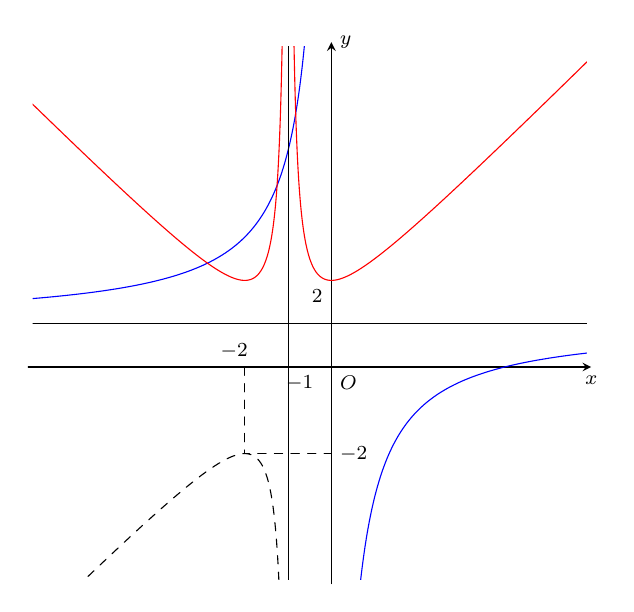
\begin{tikzpicture}[scale=0.55,>=stealth, font=\footnotesize, line join=round, line cap=round,declare function={a=1;b=2;c=2;d1=1;e1=1;xmin=-7;xmax=6;ymin=-5;ymax=7.5;f(\x)=(a*(\x)^2+b*(\x)+c)/(d1*(\x)+e1);g(\x)=((\x)-4)/(\x);} ]
\draw[->] (xmin,0)--(xmax,0) node [below]{$x$};
\draw[->] (0,ymin)--(0,ymax) node [right]{$y$};
\node at (0,0) [below right]{$O$};
\clip (xmin+0.1,ymin+0.1) rectangle (xmax-0.1,ymax-0.1);
\draw[dashed,smooth,samples=300,domain=xmin:(-e1/d1-0.1)] plot(\x,{f(\x)});
\draw[blue,smooth,samples=300,domain=xmin:-0.1] plot(\x,{g(\x)});
\draw[blue,smooth,samples=300,domain=0.1:xmax] plot(\x,{g(\x)});
\draw[red,smooth,samples=300,domain=(-e1/d1+0.1:xmax)] plot(\x,{f(\x)});
\draw (-e1/d1,ymin)--(-e1/d1,ymax) (xmin,1)--(xmax,1);
\draw[red,smooth,samples=300,domain=xmin:(-e1/d1-0.1)] plot(\x,{-f(\x)});
\draw[dashed] (0,2)node[below left]{$2$} (-2,0)node[above,xshift=-0.15cm]{$-2$}--(-2,-2)--(0,-2)node[right]{$-2$} (-1,0)node[below right,xshift=-0.15cm]{$-1$};
\end{tikzpicture}
\end{center}
Quan sát đồ thị ta thấy đồ thị hàm số $y=|f(x)|$ và đồ thị hàm số $y=\dfrac{x-4}{x}$ cắt nhau tại ba điểm phân biệt.\\ Do đó phương trình $x\cdot\left|f(x)\right|=x-4$ có đúng $3$ nghiệm thực phân biệt
\end{itemchoice}
}
\end{ex}

\begin{ex} %[2D1V3-6]
Khi thả một quả bóng từ đỉnh một toà tháp xuống, nó chạm đất sau 3 giây. Sau đó, quả bóng nảy lên trước khi chạm đất lần nữa 4 giây sau đó. Chiều cao tinh bằng mét của quả bóng so với mặt đất sau $t$ giây tuân theo một hàm số liên tục trên $[0; 7]$ như sau:
\[
H(t)=\left\{\begin{array}{lll}-5 t^2+c & \text{khi} & 0 \leq t < 3 \\-5 t^2+d t+e & \text{khi} & 3 \leq t \leq 7
\end{array}(c, d, e \in \mathbb{R}).\right.
\]
\begin{center}
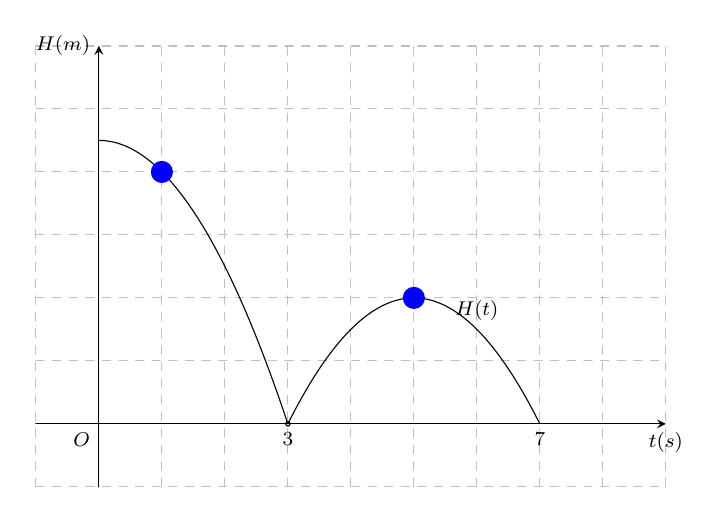
\begin{tikzpicture}[scale=0.8,>=stealth, font=\footnotesize, line join=round, line cap=round]
\def\a{-0.5} \def\b{0} \def\c{4.5} % Hệ số
\def\xmin{-1} \def\xmax{9}
\def\ymin{-1} \def\ymax{6}
\draw[color=gray!50,dashed] (\xmin,\ymin) grid (\xmax,\ymax);
\draw[->] (\xmin,0)--(\xmax,0) node [below]{$t(s)$};
\draw[->] (0,\ymin)--(0,\ymax) node [left]{$H(m)$};
\node at (0,0) [below left]{$O$};
\clip (\xmin+0.1,\ymin+0.1) rectangle (\xmax-0.5,\ymax-0.1);
\draw[smooth,samples=300,domain=0:3] plot(\x,{\a*(\x)^2+\b*(\x)+\c});
\draw[smooth,samples=300,domain=3:7] plot(\x,{-0.5*(\x)^2+5*(\x)-10.5});
\fill[blue] (1,4) circle (5pt);
\fill[blue] (5,2) circle (5pt);
\draw (3,0) circle (1pt);
\draw (6,1.5)  node [above]{$H(t)$};
\draw (3,0)  node [below]{$3$};
\draw (7,0)  node [below]{$7$};
\end{tikzpicture}
\end{center}
\choiceTF
{\True $H(3)=H(7)=0$}
{Quả bóng được thả từ độ cao $40$ m}
{Giá trị của $d$ là $d=100$}
{\True Độ cao lớn nhắt mà quả bóng đạt được sau lần nảy đầu tiên là $20$ m}
\loigiai{
\begin{itemchoice}
\itemch Dựa vào đôg thị ta có $H(3)=H(7)=0$.
\itemch Quả bóng được thả tại thời điểm $t=0$, nên để tìm độ cao của quả bóng ta tìm $H(0)$.\\
Vì hàm số liên tục tại $x=3$ nên $\lim\limits_{x\to3}H(t)=H(3)\Leftrightarrow -5\cdot3^2+c=0\Leftrightarrow c=45
$.\\
Vậy $H(0)=45$. Do đó quả bóng được thả từ độ cao $45$ m.
\itemch
Ta có $\heva{&H(3)=0\\&H(7)=0}\Leftrightarrow \heva{&-5\cdot3^2+3d+e=0\\&-5\cdot7^2+7d+e=0}\Leftrightarrow \heva{&d=50\\&e=-105.}$\\
Vậy $H(t)=-5t^2+50t-105$.
\itemch
Độ cao của quả bóng sau lần nảy đầu tiên trong khoảng thời gian $t\in[3;7]$ nên được mô tả bởi $H(t)=-5t^2+50t-105$.\\
$H'(t)=-10t+50=0\Leftrightarrow t=5$ (tm).\\
Ta có $H(3)=H(7)=0$; $H(5)=20$.\\
Vậy độ cao lớn nhất của quả bóng sau lần nảy đầu tiên là $20$ m.
\end{itemchoice}

}
\end{ex}

\begin{ex}%[2D1V3-6]%[Tex đề Moon 2025]%[Nguyễn Hồng Thạch]
Trong một số trường hợp, tin đồn lan truyền và được mô hình hóa bằng hàm số\break $p(t)=\dfrac{1}{1+a\cdot\mathrm{e}^{-kt}}$, trong đó $p(t)$ là tỉ lệ dân số biết tin đồn tại thời điểm $t$ (giờ) và $a$, $k$ là hằng số dương. Giả sử $a=10$ và $k=0{,}5$. Khi đó
\choiceTF
{\True $\lim\limits_{t\to+\infty}p(t)=1$}
{Tốc độ lan truyền tin đồn là $p'(t)=\dfrac{10\mathrm{e}^{-0{,}5t}}{\left(1+10\mathrm{e}^{-0{,}5t}\right)^2}$}
{Tốc độ lan truyền tin đồn lớn nhất sau $9{,}2$ giờ (kết quả làm tròn đến hàng phần mười)}
{\True Tại thời điểm tin đồn lan truyền với tốc độ lớn nhất thì có $50\%$ dân số biết tin đồn (làm tròn kết quả đến hàng đơn vị)}
\loigiai{
\begin{itemchoice}
\itemch Vì $\lim\limits_{t \to +\infty} \mathrm{e}^{-0{,}5t} = 0 \Rightarrow \lim\limits_{t \to +\infty} p(t) = \dfrac{1}{1 + 10 \cdot 0} = 1$.
\itemch Ta có
\[
p(t) = \dfrac{1}{1 + 10\mathrm{e}^{-0{,}5t}} \Rightarrow p'(t) = \dfrac{10 \cdot 0{,}5 \mathrm{e}^{-0{,}5t}}{(1 + 10\mathrm{e}^{-0{,}5t})^2} = \dfrac{5\mathrm{e}^{-0{,}5t}}{(1 + 10\mathrm{e}^{-0{,}5t})^2}.
\]
\itemch Ta có \begin{eqnarray*}
p''(t)&=&\dfrac{-2{,}5\mathrm{e}^{-0{,}5t}\left(1+10\mathrm{e}^{-0{,}5t}\right)^2-2\left(1+10\mathrm{e}^{-0{,}5t}\right)\cdot\left(-5\mathrm{e}^{-0{,}5t}\right)\cdot 5\mathrm{e}^{-0{,}5t}}{\left(1+10\mathrm{e}^{-0{,}5t}\right)^4}\\
&=&\dfrac{-2{,5}\mathrm{e}^{-0{,}5t}+25\mathrm{e}^{-t}}{\left(1+10\mathrm{e}^{-0{,}5t}\right)^3}
\end{eqnarray*}
Suy ra \[p''(t)=0\Leftrightarrow-2{,5}\mathrm{e}^{-0{,}5t}+25\mathrm{e}^{-t}=0\Leftrightarrow \mathrm{e}^{-0{,}5t}=\dfrac{1}{10}\Leftrightarrow t=\dfrac{\ln 10}{0{,}5}\approx4{,}6.\]
Ta có 	\begin{center}

\begin{tikzpicture}[scale=0.8]
\tkzTabInit
[lgt=1.2,espcl=2.5] % tùy chọn
{$t$/1,$p''(t) $/1,$p'(t)$/2.5}
{$0$,$\tfrac{\ln10}{0{,}5}$,$+\infty$}
\tkzTabLine{,-,0,+,} %
\tkzTabVar{-/, +/,-/} %dấu mũi tên, + trên, -dưới
\end{tikzpicture}
\end{center}
Dựa vào bảng biến thiên ta thấy tốc độ lan truyền lớn nhất tại thời điểm $t\approx 4{,}6$ giờ.
\itemch Thay $t = \dfrac{\ln 10}{0{,}5}$ vào $p(t)$:
\[
p\left(\dfrac{\ln 10}{0{,}5}\right) = \dfrac{1}{1 + 10e^{-0{,}5 \cdot \tfrac{\ln 10}{0{,}5}}} = \dfrac{1}{1 + 10 \cdot \dfrac{1}{10}} = \dfrac{1}{2} = 50\%.
\]
\end{itemchoice}
}
\end{ex}

\begin{ex}%[2D1V3-6]%[TEX Đề Moon 2025]%[Võ Nguyên Thạch]
Một nhà sản xuất trung bình bán được $1\,000$ ti vi màn hình phẳng mỗi tuần với giá $14$ triệu đồng một chiếc. Một cuộc khảo sát thị trường chỉ ra rằng nếu cứ giảm giá bán $500$ nghìn đồng, số lượng ti vi bán ra sẽ tăng thêm khoảng $100$ ti vi mỗi tuần. Gọi $x$ là số ti vi bán được mỗi tuần, $p$ (triệu đồng) là giá bán của mỗi ti vi. Khi đó $p=p(x)$ được gọi là hàm cầu.
\choiceTF
{\True Hàm cầu là $p=-\dfrac{1}{200}x+19$ (triệu đồng)}
{Tổng doanh thu từ tiền bán ti vi là $200p^2+3\,800p$ (triệu đồng)}
{\True Công ty giảm giá $4{,}5$ triệu đồng cho người mua thì doanh thu của công ty sẽ lớn nhất}
{\True Nếu hàm chi phí hằng tuần là $C(x)=12\,000-3x$ (triệu đồng), trong đó $x$ là số ti vi bán ra trong tuần, nhà sản xuất nên đặt giá bán $8$ triệu đồng thì lợi nhuận là lớn nhất}
\loigiai{
\begin{itemchoice}
\itemch Theo giả thiết, tốc độ thay đổi của $x$ tỉ lệ với tốc độ thay đổi của $p$ nên hàm số $p=p(x)$ là hàm số bậc nhất.\\
Khi đó, $p(x)=ax+b$, ($a$ khác $0$).\\
Giá tiền $p_1=14$ ứng với $x_1=1\,000$; giá tiền $p_2=13{,}5$ ứng với $x_2=1\,000+100=1\,100$.\\
Do đó phương trình đường thẳng $p(x)=ax+b$ đi qua hai điểm $(1\,000;14)$ và $(1\,100;13{,}5)$.\\
Ta có hệ phương trình $\heva{&14=1\,000a+b\\&13{,}5=1\,100a+b}\Leftrightarrow \heva{&a=-\dfrac{1}{200}\\&b=19}$ (thỏa mãn).\\
Vậy hàm cầu là
\[p(x)=-\dfrac{1}{200}x+19.\]
\itemch Ta có $p=-\dfrac{1}{200}x+19\Rightarrow x=-200p+3\,00$.\\
Suy ra Tổng doanh thu từ tiền bán ti vi là
\[R(x)=px=p(-200p+3\,800)=-200p^2+3\,800p \text{ (triệu đồng).}\]
\itemch Để doanh thu là lớn nhất thì ta cần tìm $p$ sao cho $R$ đạt giá trị lớn nhất.\\
Ta có $R'=-400p+3\,800=0\Rightarrow p=\dfrac{19}{2}$.\\
Bảng biến thiên
\begin{center}

\begin{tikzpicture}
\tkzTabInit[espcl=2.5,lgt=1.5,nocadre]
{$p$/0.9,$R'(p)$/0.7,$R(x)$/2.1}
{$0$,$\dfrac{19}{2}$,$+\infty$}
\tkzTabLine{,+,0,-,}
\tkzTabVar{-/$0$,+/$18\,050$,-/$-\infty$}
\end{tikzpicture}
\end{center}
Vậy công ty nên giảm giá số tiền một chiếc ti vi là $14-\dfrac{19}{2}=4{,}5$ (triệu đồng) thì doanh thu là lớn nhất.
\itemch Doanh thu bán hàng của x sản phẩm là
\[R(x)=x\cdot p(x)=x\cdot \left(-\dfrac{1}{200}x+19\right)=-\dfrac{x^2}{200}+19x \text{ (triệu đồng).}\]
Do đó hàm số thể hiện lợi nhuận thu được khi bán $x$ sản phẩm là
\[P(x)=R(x)-C(x)=-\dfrac{x^2}{200}+19x-12\,000+3x=-\dfrac{x^2}{200}+22x-12\,000 \text{ (triệu đồng).}\]
Để lợi nhuận là lớn nhất thì $P(x)$ là lớn nhất.\\
Ta có $P'(x)=-\dfrac{x}{100}+22=0\Leftrightarrow x=2\,200$.\\
Bảng biến thiên:
\begin{center}

\begin{tikzpicture}
\tkzTabInit[espcl=2.5,lgt=1.5,nocadre]
{$x$/0.7,$P'(x)$/0.7,$P(x)$/2.1}
{$0$,$22\,$,$+\infty$}
\tkzTabLine{,+,0,-,}
\tkzTabVar{-/$0$,+/$12\,000$,-/$-\infty$}
\end{tikzpicture}
\end{center}
Vậy có $2\,200$ ti vi được bán ra thì lợi nhuận là cao nhất. Số ti vi mua tăng lên là $2\,200-1\,000=1\,200$ (chiếc).\\
Vậy cửa hàng nên đặt giá bán là $14-0{,}5\cdot \dfrac{1\,200}{100}=8 \text{ (triệu đồng)}$.
\end{itemchoice}
}
\end{ex}

\begin{ex}%[2D1V2-2]%[TEX ĐỀ MOON 2025]%[Lê Hữu Kiệt]
\immini[thm]
{Cho hàm số $y=f(x)$ có đạo hàm trên $\mathbb{R}$ và hàm số $y=f'(x)$ là hàm số bậc ba có đồ thị là đường cong trong hình vẽ.
\choiceTF
{Hàm số $y=f(x)$ đồng biến trên khoảng $(-\infty;-2)$}
{Hàm số $y=f(x)$ có hai điểm cực trị}
{$f'(2)=4$}
{\True Hàm số $g(x)=f(x)-\dfrac{1}{2}x^2+x+2024$ đồng biến trên khoảng $\left(-\dfrac{5}{2};-\dfrac{3}{2}\right)$}
}
{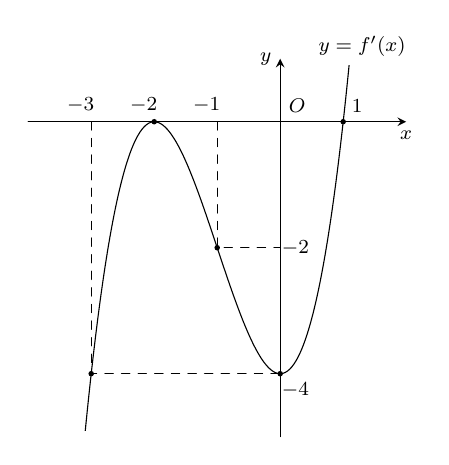
\begin{tikzpicture}[scale=0.8,>=stealth, font=\footnotesize, line join=round, line cap=round]
\def\a{1} \def\b{3} \def\c{0} \def\d{-4} % Hệ số
\def\xmin{-4} \def\xmax{2}
\def\ymin{-5} \def\ymax{1}
\draw[->] (\xmin,0)--(\xmax,0) node [below]{$x$};
\draw[->] (0,\ymin)--(0,\ymax) node [left]{$y$};
\node at (0,0) [above right]{$O$};
\draw (1.3,1.2)node[]{$y=f'(x)$};
\clip (\xmin+0.1,\ymin+0.1) rectangle (\xmax-0.5,\ymax-0.1);
\draw[smooth,samples=300] plot(\x,{\a*(\x)^3+\b*(\x)^2+\c*(\x)+\d});
\draw[dashed] (-3,0)node[above,xshift=-0.15cm]{$-3$}--(-3,-4)--(0,-4)node[below right,xshift=-0.1cm]{$-4$} (-2,0)node[above,xshift=-0.15cm]{$-2$} (-1,0)node[above,xshift=-0.15cm]{$-1$}--(-1,-2)--(0,-2)node[right,xshift=-0.1cm]{$-2$} (1,0)node[above right]{$1$};
\foreach \x/\y in {-3/-4, -2/0, -1/-2, 0/-4, 1/0}{\fill (\x,\y) circle (1.25pt);}
\end{tikzpicture}}
\loigiai{
\begin{itemchoice}
\itemch Ta có $f'(x)<0$, $\forall x\in (-\infty;-2)$ nên $y=f(x)$ nghịch biến trên khoảng $(-\infty;-2)$.
\itemch Ta có $y=f'(x)$ chỉ đổi dấu khi qua điểm $x=1$ nên hàm số có $1$ điểm cực trị.
\itemch Gọi $y=f'(x)=ax^3+bx^2+cx+d$ ($a\ne0$). Ta có đồ thị hàm số $y=f'(x)$ đi qua các điểm có tọa độ $(-3;-2)$, $(-2;0)$, $(-1;-2)$ và $(0;-4)$ nên ta có hệ phương trình
\[\heva{&-81a+27b-9c+d=-4\\&-8a+4b-2c+d=0\\&-a+b-c+d=-2\\&d=-4} \Leftrightarrow \heva{&a=1\\&b=3\\&c=0\\&d=-4.}\]
Suy ra $y=f'(x)=x^3+3x^2-4$.\\
Khi đó $f'(2)=16$.
\itemch Ta có $g'(x)=f'(x)-x+1=x^3+3x^2-x-3$.\\
Khi đó $g'(x)=0\Leftrightarrow x^3+3x^2-x-3=0 \Leftrightarrow \hoac{&x=-3\\&x=-1\\&x=1.}$\\
Bảng biến thiên
\begin{center}

\begin{tikzpicture}[font=\footnotesize, line join=round, line cap=round, >=stealth, scale=1]
\tkzTabInit[espcl=2.5,lgt=1.5]
{$x$/0.7,$g'(x)$/0.7,$g(x)$/2}
{$-\infty$, $-3$, $-1$, $1$, $+\infty$}
\tkzTabLine{,-,$0$,+,$0$,-,$0$,+,}
\tkzTabVar{+/, -/, +/, -/, +/}
\end{tikzpicture}
\end{center}
Suy ra hàm số $y=g(x)$ đồng biến trên các khoảng $(-3;-1)$, $(1;+\infty)$.\\
Mà $\left(-\dfrac{5}{2};-\dfrac{3}{2}\right)\subset(-3;-1)$ nên hàm số $y=g(x)$ đồng biến trên khoảng $\left(-\dfrac{5}{2};-\dfrac{3}{2}\right)$.
\end{itemchoice}
}
\end{ex}

\begin{ex}%[2D1V3-6]
\immini{Người ta muốn thiết kế một lồng nuôi cá có bề mặt hình chữ nhật bao gồm phần mặt nước có diện tích bằng $54$ m$^2$ và phần đường đi xung quanh với kích thước (đơn vị: m) như hình vẽ
\choiceTF
{\True Kích thước hình chữ nhật phần mặt nước là $(a-3)$ (m) và $(b-2)$ (m), với $a>3$, $b>2$}
{ Biểu diễn $b$ theo $a$ là $b=\dfrac{54}{a-2}+3$}
{Diện tích phần đường đi theo $a$ là $S(a)=\dfrac{54a}{a-3}+3a-5$, $(a>3)$}
{\True Diện tích phần đường đi là bé nhất bằng $42$ (m$^2$)}}{
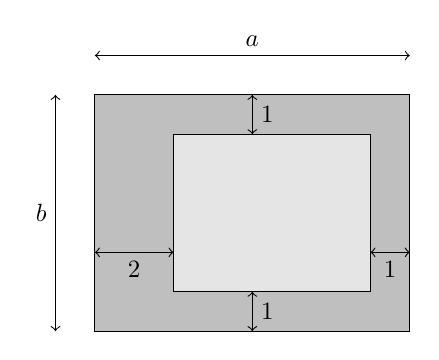
\begin{tikzpicture}
\coordinate (A) at (0,0);
\coordinate (B) at (4,0);
\coordinate (C) at (4,3);
\coordinate (D) at (0,3);
\fill[draw=black, fill=gray!50] (A) rectangle (C) ;
\fill[draw=black, fill=gray!20] (1,0.5)--(3.5,0.5)--(3.5,2.5)--(1,2.5)--cycle;
\draw[<->] (0,3.5)--node[above]{$a$}(4,3.5);
\draw[<->] (-0.5,0)--node[left]{$b$}(-0.5,3);
\draw[<->] (0,1)--node[below]{$2$}(1,1);
\draw[<->] (3.5,1)--node[below]{$1$}(4,1);
\draw[<->] (2,0)--node[right]{$1$}(2,0.5);
\draw[<->] (2,2.5)--node[right]{$1$}(2,3);
\end{tikzpicture}
}
\loigiai{
\begin{itemchoice}
\itemch Kích thước hình chữ nhật phần mặt nước là $(a-3)$ (m) và $(b-2)$ (m), với $a>3$, $b>2$.
\itemch Diện tích phần mặt nước là $54$ (m$^2$) nên \[(a-3)(b-2)=54\Leftrightarrow b-2=\dfrac{54}{a-3}\Leftrightarrow b=\dfrac{54}{a-3}+2.\]
\itemch Diện tích cá lồng nuôi cá là \[a\cdot b=a\cdot\left(\dfrac{54}{a-3}+2\right)=\dfrac{54a}{a-3}+2a.\]
Diện tích phần đường đi là $\dfrac{54a}{a-3}+2a-54$.
\itemch Xét hàm số $f(a)=\dfrac{54a}{a-3}+2a-54\Rightarrow f'(a)=\dfrac{-162}{(a-3)^2}+2$.\\
Ta có $f'(a)=0\Leftrightarrow a=-6$ (loại) hoặc $a=12$ (thoả mãn).\\
Tính giá trị của $f(a)$ tại điểm cực trị, ta có diện tích phần đường đi nhó nhất khi $a=12$ (m) và có diện tích $f(12)=42$ (m$^2$).
\end{itemchoice}
}
\end{ex}

% \paragraph{Mức độ C}
\begin{ex}%[50 Đề minh họa tốt nghiệp 2025 - Đề 13]%[Lê Hữu Kiệt - Lê Quân]%[2D1C2-7]
Trên trục $Os$, cho hai chất điểm chuyển động có toạ độ theo thời gian $t$ (giây) lần lượt là $s_1=\sin t$ và $s_2=\sin\left(t+\dfrac{\pi}{3}\right)$ (đơn vị: mét).
\begin{center}
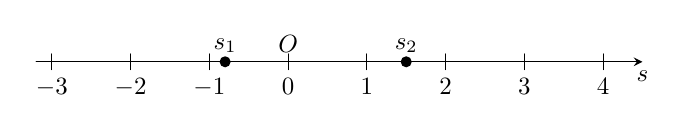
\begin{tikzpicture}[line join=round, line cap=round, >=stealth, scale=1]
\draw[->] (-3.2,0)--(4.5,0)node[below]{$s$};
\draw (0,0)node[above]{$O$};
\fill (-0.8,0) circle (2pt) node[above]{$s_1$} (1.5,0) circle (2pt) node[above]{$s_2$};
\foreach \x in {-3,...,4}{
\draw (\x,0.1)--(\x,-0.1)node[below]{$\x$};
}
\end{tikzpicture}
\end{center}
\choiceTF
{Tại thời điểm ban đầu hai chất điểm cách nhau một khoảng bằng $50$ cm}
{Khoảng cách giữa hai chất điểm được xác định bởi hàm số $d=s_1-s_2$ (mét)}
{\True Trong $6$ giây đầu tiên, có hai thời điểm mà vận tốc của hai chất điểm bằng nhau}
{\True Trong $6$ giây đầu tiên, khoảng cách xa nhất của hai chất điểm là $100$ cm}
\loigiai{
\begin{itemchoice}
\itemch Tại thời điểm bắt đầu thì $t=0$. Khi đó $s_1=\sin 0 = 0$; $s_2=\sin\left(0+\dfrac{\pi}{3}\right)=\dfrac{\sqrt3}{2}$.\\
Khoảng cách giữa hai chất điểm là $s_2-s_1=\dfrac{\sqrt3}{2}$ m.
\itemch Khoảng cách giữa hai chất điểm được xác định bởi hàm số $d=|s_1-s_2|$ (mét).
\itemch Vận tốc của chất điểm thứ nhất và thứ hai lần lượt là $v_1=s_1'=\cos t$ và $v_2=s_2'=\cos\left(t+\dfrac{\pi}{3}\right)$.\\
Khi hai chất điểm có vận tốc bằng nhau
\begin{eqnarray*}
&& v_1=v_2 \\
&\Leftrightarrow& \cos t = \cos\left(t+\dfrac{\pi}{3}\right) \\
&\Leftrightarrow& \hoac{&t=t+\dfrac{\pi}{3}+k2\pi \\& t=-t-\dfrac{\pi}{3}+k2\pi} \\
&\Leftrightarrow& t=-\dfrac{\pi}{6}+k\pi,\, (k\in\mathbb{Z}).
\end{eqnarray*}
Trong $6$ giây đầu tiên, tức $0\leq t \leq 6 \Leftrightarrow 0\leq -\dfrac{\pi}{6}+k\pi \leq 6 \Leftrightarrow \dfrac{1}{6} \leq k < 2{,}08$.\\
Do $k\in\mathbb{Z}$ nên $k\in\{1;2\}$.\\
Vậy trong $6$ giây đầu tiên, có hai thời điểm mà vận tốc của hai chất điểm bằng nhau.
\itemch Xét $y=s_1-s_2=\sin t - \sin\left(t+\dfrac{\pi}{3}\right)$.\\
Tập xác định $\mathscr{D}=\mathbb{R}$.\\
Ta có $y'=\cos t - \cos\left(t+\dfrac{\pi}{3}\right)$.\\
Cho $y'=0 \Leftrightarrow \cos t- \cos\left(t+\dfrac{\pi}{3}\right)=0 \Leftrightarrow t=-\dfrac{\pi}{6}+k\pi$, $k\in\mathbb{Z}$.\\
Bảng biến thiên của $y$ trên đoạn $[0;6]$
\begin{center}

\begin{tikzpicture}[font=\footnotesize, line join=round, line cap=round, >=stealth, scale=1]
\tkzTabInit[lgt=1.2,espcl=2.5,deltacl=0.6]
{$x$/1, $y'$/0.7, $y$/2}
{$0$, $\dfrac{5\pi}{6}$, $\dfrac{11\pi}{6}$, $6$}
\tkzTabLine
{, + , $0$ , - , $0$ , + , }
\tkzTabVar
{-/$-\dfrac{\sqrt3}{2}$ , +/$1$, -/$-1$, +/$-0{,}97$}
\end{tikzpicture}
\end{center}
Suy ra, khoảng cách giữa hai chất điểm là $d=|y|$ có giá trị lớn nhất là $1$ m, hay $100$ cm khi $t=\dfrac{5\pi}{6}$ và $t=\dfrac{11\pi}{6}$.\\
\end{itemchoice}
}
\end{ex}


\Closesolutionfile{ans}

\Opensolutionfile{ans}[ans/ansBTshortans]

\subsection{Câu trắc nghiệm trả lời ngắn}
% \paragraph{Mức độ N}
% \paragraph{Mức độ H}
\setcounter{ex}{0}
\begin{ex}%[1H8H5-4]%[TEX ĐỀ MOON 2025]%[Nguyễn Văn Hiệp]
Cho hình lăng trụ đứng $ABC.A'B'C'$ có đáy là tam giác đều độ dài cạnh bằng $6\sqrt{3}$. Khoảng cách giữa hai đường thẳng $AA'$ và $BC$ bằng bao nhiêu?
\shortans{$9$}
\loigiai{\immini{ \textbf{Bước 1: Xác định hình chiếu vuông góc} \\
Vì lăng trụ đứng nên $AA' \perp (ABC)$. Gọi $M$ là trung điểm $BC$, ta có $AM \perp BC$.\\
\textbf{Bước 2: Tính độ dài đường cao} \\
Tam giác $ABC$ đều cạnh $6\sqrt{3}$ có
\[
AM = \dfrac{6\sqrt{3} \cdot \sqrt{3}}{2} = 9.
\]
\textbf{Bước 3: Kết luận khoảng cách} \\
Vì $AA' \perp (ABC)$ và $AM \perp BC$ nên
\[
\mathrm{d}(AA', BC) = AM = 9.
\]}{\begin{tikzpicture}[line join=round, line cap=round,>=stealth,thick,scale=0.8,font=\scriptsize]
\def\a{4}
\def\h{4.5}
\path 	(0:0) coordinate (A)
++(0:\a) coordinate (C)
++(-150:3*\a/4) coordinate (B)
($(A)+(90:\h)$) coordinate (A')
($(B)+(90:\h)$) coordinate (B')
($(C)+(90:\h)$) coordinate (C')
($(B)!0.5!(C)$) coordinate (M)
;
\draw[dashed,thick] 	(A)--(C) (A)--(M);
\draw[thick]	(C)--(C') 	(B)--(B')	(A)--(A') (A)--(B)--(C) (A')--(B')--(C')--cycle;
\foreach \x/\g in {A/180,B/-45,C/0,A'/180,B'/-45,C'/0,M/-45}
\fill[black] 	(\x) circle (1pt)
($(\g:4mm)+(\x)$) node {$\x$};
\end{tikzpicture}
}

}
\end{ex}

\begin{ex}%[1H8H5-4]%[TEX ĐỀ MOON 2025]%[Nguyễn Cường]
Cho hình lăng trụ đứng $ABC.A'B'C'$ có $AB=5$, $AC=6$, $\widehat{A}=60^\circ$. Khoảng cách giữa hai đường thẳng $AA'$ và $BC$ (làm tròn kết quả đến hàng phần mười) bằng bao nhiêu?
\shortans{$4{,}7$}
\loigiai
{
\begin{center}
\begin{tikzpicture}[scale=1, font=\footnotesize, line join=round, line cap=round, >=stealth]
\path
(0,0)coordinate(A)++(0:4)coordinate(C)++(210:3)coordinate(B)
(A)++(90:3)coordinate(A')++(0:4)coordinate(C')++(210:3)coordinate(B')
($(B)!.4!(C)$)coordinate(H)
;
\draw (A')--(A)--(B)--(C)--(C')--(B')--(A')--(C')
(B)--(B')
;
\draw[dashed] (H)--(A)--(C);
\foreach \i/\g in {A/180,B/-90,C/0,A'/90,B'/90,C'/90,H/-90}{\draw[fill=black](\i) circle (1pt) ($(\i)+(\g:3mm)$) node[scale=1]{$\i$};}
\end{tikzpicture}
\end{center}
Gọi $AH$ là đường cao của $\triangle ABC$.\\
Ta có $\heva{&AA'\perp AH\\&BC\perp AH}\Rightarrow \mathrm{d}\big(AA',BC\big)=AH$.\\
Xét $\triangle ABC$ có
\begin{itemize}
\item $BC=\sqrt{AB^2+AC^2-2AB\cdot AC\cos\widehat{A}}=\sqrt{25+36-2\cdot 5\cdot 6\cdot \cos 60^\circ}=\sqrt{31}$.
\item $AH=\dfrac{AB\cdot AC\cdot\sin 60^\circ}{BC}=\dfrac{5\cdot 6\cdot \sin 60^\circ}{\sqrt{31}}=\dfrac{15\sqrt{93}}{31}\approx 4{,}67$.
\end{itemize}
Vậy $\mathrm{d}\big(AA',BC\big)=AH\approx 4{,}67$.
}
\end{ex}

\begin{ex}%[1H8H5-3]
Cho hình chóp $S.ABCD$ có đáy là hình vuông cạnh bằng $1$, $SA$ vuông góc với mặt phẳng $(ABCD)$ và $SA=\dfrac{\sqrt{3}}{3}$. Khoảng cách từ điểm $A$ đến mặt phẳng $(SCD)$ bằng bao nhiêu? (làm tròn kết quả đến hàng phần mười).
\shortans{0{,}5}
\loigiai{
\immini{
Ta có $\heva{& CD \perp AD \\ & CD \perp SA \\ & AD, SA \subset (SAD) \\ & AD \cap SA = \{A\}} \Rightarrow CD \perp (SAD)$. \\
Trong mặt phẳng $(SAD)$, kẻ $AH \perp SD$ tại $H$. \\
Vì $CD \perp (SAD)$ và $AH \subset (SAD)$ nên $CD \perp AH$. \\
Ta có $\heva{& AH \perp SD \\ & AH \perp CD \\ & SD, CD \subset (SCD) \\ & SD \cap CD = \{D\}} \Rightarrow AH \perp (SCD)$. \\
Do đó, khoảng cách từ điểm $A$ đến mặt phẳng $(SCD)$ là $\mathrm{d}(A, (SCD)) = AH$. \\
Xét tam giác $\triangle SAD$ vuông tại $A$, có $AD=1$ và $SA=\dfrac{\sqrt{3}}{3}$. \\
Áp dụng hệ thức lượng trong tam giác vuông $SAD$, ta có \\
$\dfrac{1}{AH^2} = \dfrac{1}{SA^2} + \dfrac{1}{AD^2} = \dfrac{1}{\left(\dfrac{\sqrt{3}}{3}\right)^2} + \dfrac{1}{1^2} = \dfrac{1}{\frac{3}{9}} + 1 = \dfrac{1}{\frac{1}{3}} + 1 = 3 + 1 = 4$. \\
$\Rightarrow AH^2 = \dfrac{1}{4} \Rightarrow AH = \dfrac{1}{2} = 0{,}5$. \\
Vậy khoảng cách từ điểm $A$ đến mặt phẳng $(SCD)$ bằng $0{,}5$.
}{
\begin{tikzpicture}[>=stealth,line join=round,line cap=round,font=\footnotesize,scale=1]
\tikzset{
pics/hinhChopTuGiac/.style  n args={5}{
code={
\tikzset{
declare function={a=4;b=2;h=3;goc=-120;}
}
\path
(0,0)coordinate (#1)+(0:a)coordinate (#2)+(goc:b)coordinate (#4)+(90:h)coordinate (#5)
($(#2)+(#4)-(#1)$)coordinate (#3)
;
}
}}
\path
(0,0)pic {hinhChopTuGiac={A}{D}{C}{B}{S}}
($(S)!.4!(D)$)coordinate (H)
pic[draw,angle radius=2mm,angle eccentricity=1.5]{right angle=A--H--D}
;
\foreach \pointo/\pointt in {S/B,S/C,S/D,B/C,C/D}{
\draw[fill=black](\pointo)--(\pointt);
}
\foreach \pointo/\pointt in {S/A,A/B,A/D,A/H}{
\draw[fill=black,dashed](\pointo)--(\pointt);
}
\foreach \point/\goc in {A/160,S/90,B/190,D/10,C/-45,H/45}{
\draw[fill=black](\point)circle(.8pt)+(\goc:2mm)node[scale=.8]{$\point$};
}
\end{tikzpicture}
}

}
\end{ex}

\begin{ex}%[1D6H4-6]%[TEX ĐỀ MOON 2025]%[Lê Hữu Kiệt]
Các khí thải gây hiệu ứng nhà kính là nguyên nhân chủ yếu làm Trái Đất nóng lên. Theo OECD (Tổ chức Hợp tác và Phát triển kinh tế Thế giới), khi nhiệt độ Trái Đất tăng lên thì tổng giá trị kinh tế toàn cầu giảm. Người ta ước tính rằng, khi nhiệt độ Trái Đất tăng thêm $2^\circ$C thì tổng giá trị kinh tế toàn cầu giảm $3\%$; còn khi nhiệt độ Trái Đất tăng thêm $5^{\circ}$C thì tổng giá trị kinh tế toàn cầu giảm $10\%$. Biết rằng, nếu nhiệt độ Trái Đất tăng thêm $t^\circ$C, tổng giá trị kinh tế toàn cầu giảm $f(t)\%$ thì $f(t)=k\cdot a^t$, trong đó $k$, $a$ là các hằng số dương. Khi nhiệt độ Trái Đất tăng thêm bao nhiêu độ C thì tổng giá trị kinh tế toàn cầu giảm đến $20\%$ (Làm tròn đến hàng phần chục)?
\shortans{$6{,}7$}
\loigiai{
Với $t=2$ thì $f(t)=3$, suy ra $3=ka^2\Leftrightarrow k=\dfrac{3}{a^2}$.\\
Với $t=5$ thì $f(t)=10$, suy ra
\[10=ka^5\Leftrightarrow 10=3a^3 \Leftrightarrow a=\left(\dfrac{10}{3}\right)^{\tfrac{1}{3}}.\]
Suy ra $k=\dfrac{3}{\left(\dfrac{10}{3}\right)^{\tfrac{2}{3}}}.$ Do đó $f(t)=\dfrac{3}{\left(\dfrac{10}{3}\right)^{\tfrac{2}{3}}}\cdot\left(\dfrac{10}{3}\right)^{\tfrac{t}{3}}=3\cdot\left(\dfrac{10}{3}\right)^{\tfrac{t-2}{3}}$.\\
Khi kinh tế toàn cầu giảm đến $20\%$, tức $f(t)=20$, ta có
\begin{eqnarray*}
&&3\cdot\left(\dfrac{10}{3}\right)^{\tfrac{t-2}{3}}=20 \\
&\Leftrightarrow& \left(\dfrac{10}{3}\right)^{\tfrac{t-2}{3}}=\dfrac{20}{3} \\
&\Leftrightarrow& \dfrac{t-2}{3}=\log_{\tfrac{10}{3}}\dfrac{20}{3} \\
&\Leftrightarrow&t=3\log_{\tfrac{10}{3}}\dfrac{20}{3}+2 \\
&\Leftrightarrow& t\approx 6{,}7.
\end{eqnarray*}
Vậy khi nhiệt độ Trái Đất tăng thêm khoảng $6{,}7$ độ C thì tổng giá trị kinh tế toàn cầu giảm đến $20\%$.
}
\end{ex}

\begin{ex}%[1C2H3-2]%[TEX ĐỀ MOON 2025]%[Huỳnh Thanh Chí]
Một người đưa thư xuất phát từ bưu điện ở vị trí $A$, các điểm cần phát thư nằm dọc các con đường cần đi qua. Biết rằng người này phải đi trên mỗi con đường ít nhất một lần (để phát được thư cho tất cả các điểm cần phát nằm dọc theo con đường đó) và cuối cùng quay lại điểm xuất phát. Độ dài các con đường như hình vẽ (đơn vị độ dài).
\begin{center}
\begin{tikzpicture}[scale=0.75,>=stealth, font=\footnotesize, line join=round, line cap=round]
\coordinate (A) at (0,0);
\coordinate (B) at (4,0);
\coordinate (C) at (6,-1.6);
\coordinate (D) at (4,-2.6);
\coordinate (E) at (0,-3);
\draw (A)node[above]{$A$}--(B)node[above]{$B$}--(C)node[right]{$C$}--(D)node[below]{$D$}--(E)node[below]{$E$}--(A) (E)--(B)--(D) ($(A)!0.5!(B)$)node[above]{$8$} ($(B)!0.5!(C)$)node[above right]{$5$} ($(D)!0.5!(C)$)node[below right]{$2$} ($(B)!0.5!(D)$)node[right]{$4$} ($(B)!0.5!(E)$)node[above left]{$10$} ($(A)!0.5!(E)$)node[right]{$6$} ($(E)!0.5!(D)$)node[below]{$9$};
\draw (A)..controls (-0.5,-1.5) and (-0.5,-1.5)..(E) (-0.5,-1.5)node[left]{$7$};
\end{tikzpicture}
\end{center}
Hỏi tổng quãng đường người đưa thư có thể đi ngắn nhất có thể là bao nhiêu?

\shortans[]{$63$}
\loigiai{
Bài toán yêu cầu tìm chu trình Euler có độ dài nhỏ nhất.\\
Tổng độ dài các cạnh của đồ thị là: $8+5+2+4+10+6+9+7 = 51$.\\
Các đỉnh có bậc lẻ là $A$ (bậc 3), $C$ (bậc 3), $D$ (bậc 3).\\
Cần tìm đường đi ngắn nhất để nối các đỉnh bậc lẻ này.\\
Ta có các cặp đường đi:
\begin{itemize}
\item $AC = AB+BC = 8+5 = 13$.
\item $AD = AB+BD = 8+4 = 12$.
\item $CD = 2$.
\end{itemize}
Chọn $CD=2$, khi đó:
\begin{itemize}
\item $AC=13$.
\item $AD=12$.
\end{itemize}
Ta nối $CD=2$ và chọn $AC,AD$. Ta thấy chỉ cần chọn cặp $CD$ thôi, như vậy đường đi là $AC=13$ hoặc $AD=12$, nhưng tổng $CD=2$. Ta ghép $A,C$ thì tạo đường đi $AC = 13$, và chọn ghép $AD$, có $AD=12$, hoặc $AD=12$, $CD = 2$ chọn $CD$ ngắn hơn, với các cạnh là: CD nối 2 cạnh lại: $CD=2$. Và $A,C,D$ bậc lẻ cần thêm cạnh $AC$ hoăc $AD$ cho chẵn cạnh. Ta có:
\begin{itemize}
\item $AC=13$.
\item $AD=12$.
\end{itemize}
Ta ưu tiên ghép $CD$ nên là $CD=2$. Ghép $A$ vào đỉnh còn lại: chọn đỉnh cách xa 1 đoạn: chọn $AD$ hay $AC$. Theo đó ta chọn cạnh $CD$ với $AD$ hoặc $AC$. Vì $AC,AD >CD$ ta loại $AD$, chọn CD. Sau đó chọn từ $A$ đi $C$ hoặc $D$. Chọn $A,D$.

Vậy, cặp cạnh cần lặp lại có tổng độ dài nhỏ nhất là: $CD+AD= 2+12 = 14$.
Tổng quãng đường người đưa thư phải đi là: $51 + (CD+AD) =51+14 = 63$.

Vậy tổng độ dài quãng đường ngắn nhất là $63$.
}
\end{ex}

\begin{ex}%[1C2H3-1]%[TEX ĐỀ MOON 2025]%[Nguyễn Văn Hiệp]
Giả sử $4$ thành phố $A$, $B$, $C$, $D$ với khoảng cách (đơn vị: km) giữa các thành phố được cho bởi bảng sau
\begin{center}
\begin{tblr}{hlines={0.6pt},vlines={0.6pt},width=0.7\linewidth,rows={abovesep=1pt,belowsep=1pt},colspec={X[1,c]X[1,c]X[1,c]X[1,c]X[1,c]}}
& $A$ & $B$ & $C$ & $D$ \\
$A$ & $0$ & $10$ & $15$ & $20$ \\
$B$ & $10$ & $0$ & $25$ & $35$ \\
$C$ & $15$ & $25$ & $0$ & $30$ \\
$D$ & $20$ & $35$ & $30$ & $0$ \\
\end{tblr}
\end{center}
Hãy tính quãng đường ngắn nhất để đi qua tất cả các thành phố đúng một lần rồi quay lại thành phố xuất phát?
\shortans{$85$}
\loigiai{
\textbf{Bước 1: Liệt kê các chu trình Hamilton} \\
Xét tất cả các hoán vị
\begin{itemize}
\item $A \rightarrow B \rightarrow C \rightarrow D \rightarrow A$: $10 + 25 + 30 + 20 = 85$ km.
\item $A \rightarrow B \rightarrow D \rightarrow C \rightarrow A$: $10 + 35 + 30 + 15 = 90$ km.
\item $A \rightarrow C \rightarrow B \rightarrow D \rightarrow A$: $15 + 25 + 35 + 20 = 95$ km.
\item $A \rightarrow C \rightarrow D \rightarrow B \rightarrow A$: $15 + 30 + 35 + 10 = 90$ km.
\item $A \rightarrow D \rightarrow B \rightarrow C \rightarrow A$: $20 + 35 + 25 + 15 = 95$ km.
\item $A \rightarrow D \rightarrow C \rightarrow B \rightarrow A$: $20 + 30 + 25 + 10 = 85$ km.
\end{itemize}
\textbf{Bước 2: Chọn chu trình tối ưu} \\
Quãng đường ngắn nhất là $85$ km.
}
\end{ex}

\begin{ex}%[50 Đề minh họa tốt nghiệp 2025 - Đề 13]%[Lê Hữu Kiệt - Lê Quân]%[1C2H3-1]
Biểu đồ thể hiện các con đường nối giữa các thị trấn (đơn vị: km). Cán bộ thanh tra xuất phát từ thị trấn $L$ đi kiểm tra tất cả các tuyến đường nối giữa các thị trấn $M$, $N$, $O$ và quay lại $L$. Chiều dài quãng đường tối thiểu thanh tra cần phải đi là bao nhiêu km?
\begin{center}
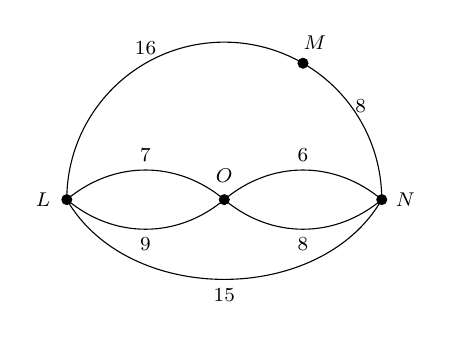
\begin{tikzpicture}[font=\footnotesize, line join=round, line cap=round, >=stealth, scale=1]
\def\bankinh{2}
\path (0,0) coordinate (O) (-\bankinh,0) coordinate (L) (\bankinh,0) coordinate (N) (60:\bankinh) coordinate (M);
\draw
(L) arc(180:60:\bankinh) node[pos=0.5, above]{$16$}
(M) arc(60:0:\bankinh) node[pos=0.5, above]{$8$}
(L) to[bend right=60] node[pos=0.5, below]{$15$} (N)
(L) to[bend right=40] node[pos=0.5, below]{$9$} (O)
(L) to[bend left=40] node[pos=0.5, above]{$7$} (O)
(O) to[bend right=40] node[pos=0.5, below]{$8$} (N)
(O) to[bend left=40] node[pos=0.5, above]{$6$} (N)
;
\foreach \x/\g in {O/90, L/180, N/0, M/60}{
\fill (\x) circle (2pt)+(\g:0.3)node{$\x$};
}
\end{tikzpicture}
\end{center}
\par\shortans{$37$}
\loigiai{
Để chiều dài quãng đường là tối thiểu, cán bộ thanh tra cần xuất phát từ $L$, đi qua mỗi thị trấn $M$, $N$, $O$ đúng một lần trước khi qua lại $L$ và ưu tiên chọn con đường ngắn hơn trong hai con đường nối hai thị trấn.\\
Ta có quãng đường tối ưu là $L\rightarrow M \rightarrow N \rightarrow O \rightarrow L$ với độ dài là $16+8+6+7=37$ km.
}
\end{ex}

\begin{ex}%[1C2H3-1]%[TEX ĐỀ MOON 2025]%[Nguyễn Cường]
\immini[thm]
{
Công ty giao hàng nhanh có $4$ kho hàng $A$, $B$, $C$ và $D$. Quản lý muốn lên kế hoạch cho xe giao hàng đi qua tất cả các kho hàng để lấy hàng và quay lại kho hàng ban đầu, với điều kiện là mỗi kho hàng chỉ ghé qua một lần. Khoảng cách giữa các kho hàng (km) được mô tả trong hình bên. Quãng đường ngắn nhất để xe giao hàng hoàn thành việc lấy hàng ở các kho và quay trở lại kho hàng ban đầu là bao nhiêu?
}
{
\begin{tikzpicture}[scale=0.8,>=stealth, font=\footnotesize, line join=round, line cap=round]
\coordinate (A) at (0,0);
\coordinate (B) at (1,-2);
\coordinate (C) at (0,-4);
\coordinate (D) at (5,-3);
\draw (A)--(C)--(D)--cycle (A)--(B)--(C) (B)--(D) ($(A)!0.5!(C)$)node[left]{$3$} ($(A)!0.5!(B)$)node[above right,yshift=-0.2cm]{$3$} ($(B)!0.5!(D)$)node[below]{$4$} ($(B)!0.5!(C)$)node[below right]{$2$} ($(C)!0.5!(D)$)node[below]{$5$} ($(A)!0.5!(D)$)node[above right]{$7$};
\foreach \x/\g in {A/90,B/180,C/-135,D/0}
\fill[black] (\x) circle(1pt) +(\g:4mm) node {$\x$};
\end{tikzpicture}
}
\shortans{$15$}
\loigiai{
\begin{itemize}
\item Lộ trình $A \to B \to C \to D \to A$.\\
Tổng quãng đường=$AB+BC+CD+DA=3+2+5+7=17$ km.
\item Lộ trình $A \to B \to D \to C \to A$.\\
Tổng quãng đường=$AB+BD+DC+CA=3+4+5+3=15$ km.
\item Lộ trình $A \to C \to B \to D \to A$.\\
Tổng quãng đường=$AC+CB+BD+DA=3+2+4+7=16$ km.
\item Lộ trình $A \to C \to D \to B \to A$.\\
Tổng quãng đường=$AC+CD+DB+BA=3+5+4+3=15$ km.
\item Lộ trình $A \to D \to B \to C \to A$.\\
Tổng quãng đường=$AD+DB+BC+CA=7+4+2+3=16$ km.
\item Lộ trình $A \to D \to C \to B \to A$.\\
Tổng quãng đường=$AD+DC+CB+BA=7+5+2+3=17$ km.
\end{itemize}
\textit{Lưu ý: Các lộ trình theo chiều ngược lại sẽ có cùng tổng độ dài.}\\
Vậy quãng đường ngắn nhất để xe giao hàng hoàn thành việc lấy hàng ở các kho và quay trở lại kho hàng ban đầu là $15$ km.
}
\end{ex}

\begin{ex}%[1H8H5-4]%[TEX ĐỀ MOON 2025]%[Huỳnh Thanh Chí]
Cho tứ diện đều $ABCD$ có cạnh $2$. Khoảng cách giữa hai đường thẳng $AB$ và $CD$ bằng bao nhiêu? (làm tròn kết quả đến hàng phần trăm).

\shortans[]{$1{,}41$}
\loigiai{
\immini{Gọi $M$, $N$ lần lượt là trung điểm $AB$ và $CD$.\\
Ta có $\triangle ACD=\triangle BCD$ nên $AN=BN$ ($2$ đường trung tuyến tương ứng).\\
Suy ra $\triangle AMB$ cân tại $M$, suy ra $MN\perp AB$.\\
Chứng minh tương tự ta có $MN\perp CD$.\\
Vậy $MN$ là đoạn vuông góc chung của $AB$ và $CD$.\\
Khi đó $MN=\mathrm{d}\left(AB,CD\right)$.
}{\begin{tikzpicture}[scale=0.9,font=\footnotesize,line join=round,line cap=round,>=stealth]
\def\a{4}
\path 	(0:0) coordinate (B)
++(0:\a) coordinate (D)
++(-120:\a/2) coordinate (C)
($(B)+(70:\a)$) coordinate (A)
($(A)!1/2!(B)$) coordinate (M)
($(C)!1/2!(D)$) coordinate (N)
;
\draw[dashed] 	(B)--(D) (M)--(N)--(B);
\draw			(B)--(A)--(D) (A)--(C) (A)--(N)
(B)--(C)--(D);
\foreach \x/\g in {A/90,B/180,C/-45,D/0,M/135,N/-45}
\fill[black] 	(\x) circle (1pt)
($(\g:3mm)+(\x)$) node {$\x$};
%Hình chóp S.ABC có SA vuông góc đáy
\end{tikzpicture}}
Xét $\triangle MBN$ vuông tại $M$ có \allowdisplaybreaks
\begin{eqnarray*}
MN&=&\sqrt{BN^2-MB^2}=\sqrt{\left(\dfrac{2\sqrt{3}}{2}\right)^2-1^2}\\
&=&\sqrt{2}\approx 1{,}41.
\end{eqnarray*}
}
\end{ex}

\begin{ex}%[1C2H2-2]%[TexDeMoon2025]%[NguyenKieuNhaTu]
Cho tứ diện $ABCD$, một con bọ đang đậu ở đỉnh $A$ của tứ diện. Mỗi lần nghe một tiếng trống thì nó nhảy sang một đỉnh bất kì của tứ diện $ABCD$ mà kề với đỉnh nó đang đậu. Hỏi sau $4$ tiếng trống nó có bao nhiêu cách trở về đỉnh $A$?
\shortans[]{$21$}
\loigiai{
Sử dụng sơ đồ cây biểu diễn các cách đi ta được $21$ cách.
\begin{center}
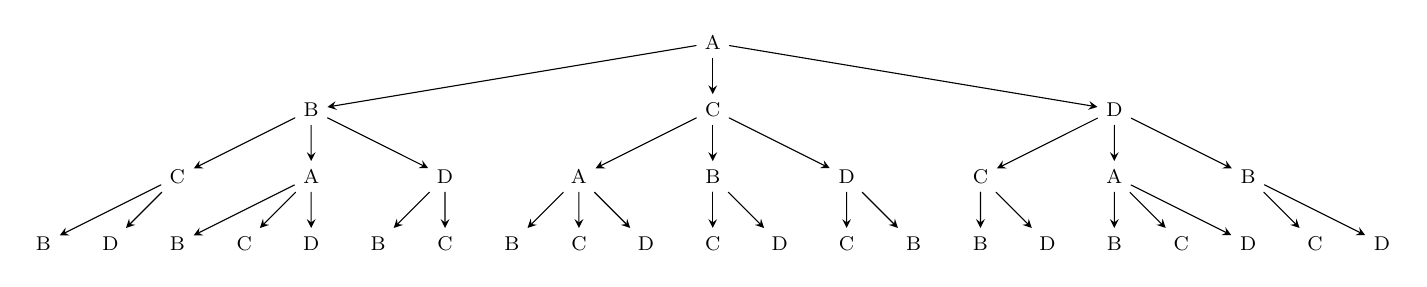
\begin{tikzpicture}[scale=.85, font=\footnotesize, line join=round, line cap=round,>=stealth]
\node (a) at (0,0) {A};
\node (d1) at (6,-1) {D};
\node (c1) at (0,-1) {C};
\node (b1) at (-6,-1) {B};
\node (c21) at (-8,-2) {C};
\node (a21) at (-6,-2) {A};
\node (d21) at (-4,-2) {D};
\node (a22) at (-2,-2) {A};
\node (b22) at (0,-2) {B};
\node (d22) at (2,-2) {D};
\node (c23) at (4,-2) {C};
\node (a23) at (6,-2) {A};
\node (b23) at (8,-2) {B};
\node (b31) at (-10,-3) {B};
\node (d31) at (-9,-3) {D};
\node (b32) at (-8,-3) {B};
\node (c32) at (-7,-3) {C};
\node (d32) at (-6,-3) {D};
\node (b33) at (-5,-3) {B};
\node (c33) at (-4,-3) {C};
\node (b43) at (-3,-3) {B};
\node (c43) at (-2,-3) {C};
\node (d43) at (-1,-3) {D};
\node (c53) at (0,-3) {C};
\node (d53) at (1,-3) {D};
\node (c63) at (2,-3) {C};
\node (b63) at (3,-3) {B};
\node (b73) at (4,-3) {B};
\node (d73) at (5,-3) {D};
\node (b83) at (6,-3) {B};
\node (c83) at (7,-3) {C};
\node (d83) at (8,-3) {D};
\node (c93) at (9,-3) {C};
\node (d93) at (10,-3) {D};

\foreach \from/\to in {a/b1,a/c1,a/d1,b1/c21,b1/a21,b1/d21,c1/a22,c1/b22,c1/d22,d1/c23,d1/a23,d1/b23,c21/b31,c21/d31,a21/b32,a21/c32,a21/d32,d21/b33,d21/c33,a22/b43,a22/c43,a22/d43,b22/c53,b22/d53,d22/c63,d22/b63,c23/b73,c23/d73,a23/b83,a23/c83,a23/d83,b23/c93,b23/d93}
\draw[->]
(\from)--(\to)
;
\end{tikzpicture}
\end{center}
}
\end{ex}

\begin{ex}%[2H5H3-1]%[TEX ĐỀ MOON 2025]%[Lê Hữu Kiệt]
Trong không gian với hệ trục tọa độ $Oxyz$, có tất cả bao nhiêu giá nguyên của $m$ để phương trình $x^2+y^2+z^2+2(m+2)x-2(m-1)z+3m^2-5=0$ là phương trình một mặt cầu?
\shortans{$7$}
\loigiai{
Phương trình có dạng $x^2+y^2+z^2-2ax-2by-2cz+d=0$ là phương trình mặt cầu khi và chỉ khi $a^2+b^2+c^2-d>0$.\\
Từ phương trình đa cho ta có $a=-(m+2)$, $b=0$, $c=m-1$ và $d=3m^2-5$.\\
Khi đó phương trình đã cho là phương trình mặt cầu khi và chỉ khi
\begin{eqnarray*}
&& [-(m+2)]^2+(m-1)^2-\left(3m^2-5\right)>0 \\
&\Leftrightarrow& -m^2+2m+10>0 \\
&\Leftrightarrow& 1-\sqrt{11}<m<1+\sqrt{11}.
\end{eqnarray*}
Do $m$ nguyên nên $m\in\{-2;-1;0;1;2;3;4\}$.\\
Vậy có $7$ giá trị nguyên của $m$ để phương trình đã cho là phương trình mặt cầu.
}
\end{ex}

\begin{ex}%[2H5H2-8]%[TEX ĐỀ MOON 2025]%[Huỳnh Thanh Chí]
Khi gắn hệ tọa độ $Oxy$ (đơn vị trên mỗi trục tính theo kilomet) vào một sân bay, mặt phẳng $(Oxy)$ trùng với mặt sân bây. Một máy bay, bay theo đường thẳng từ vị trí $A(5;0;5)$ đến vị trí $B(10;10;3)$, sau đó tiếp tục bay thẳng và hạ cánh tại vị trí $M(a;b;0)$. Giá trị của $a+b$ bằng bao nhiêu (viết kết quả dưới dạng số thập phân)?

\shortans[]{$42{,}5$}
\loigiai{
Vectơ $\overrightarrow{AB} = (10-5; 10-0; 3-5) = (5; 10; -2)$.\\
Phương trình tham số của đường thẳng $AB$ là $\heva{& x = 5 + 5t \\& y = 10t \\& z = 5 - 2t.}$\\
Vì điểm $M(a; b; 0)$ thuộc đường thẳng $AB$ và nằm trên mặt phẳng $(Oxy)$ nên $z = 0$.\\
Ta có: $5 - 2t = 0 \Rightarrow t = \dfrac{5}{2} = 2{,}5$.\\
Thay $t = 2{,}5$ vào phương trình tham số, ta được:
\[\heva{& a = 5 + 5 \cdot 2{,}5 = 17{,}5 \\
& b = 10 \cdot 2{,}5 = 25.}\]
Vậy $M(17{,}5; 25; 0)$.\\
Do đó, $a + b = 17{,}5 + 25 = 42{,}5$.
}
\end{ex}

\begin{ex}%[50 Đề minh họa tốt nghiệp 2025 - Đề 13]%[Lê Hữu Kiệt - Lê Quân]%[2H5H2-7]
Cho hình lăng trụ đứng $ABC.A'B'C'$ có đáy $ABC$ là tam giác vuông tại $C$, $AC=3a$, $BC=4a$ và góc giữa đường thẳng $B'C$ và mặt phẳng $(ABC)$ bằng $45^\circ$. Tính sin của góc giữa đường thẳng $B'C$ và mặt phẳng $(ABC')$ (làm tròn kết quả đến hàng phần trăm).
\par\shortans{$0{,}73$}
\loigiai{
Ta có $CC'\perp (ABC)$ nên $C$ là hình chiếu của $C'$ trên $(ABC)$.\\
Khi đó $\left(BC',(ABC)\right)=\left(BC',BC\right)=\widehat{C'BC}=45^\circ$.\\
Xét $\triangle C'BC$ vuông tại $C$, ta có $CC'=BC\tan\widehat{C'BC}=4a\cdot\tan 45^\circ=4a$.\\
Chọn hệ trục tọa độ $Oxyz$, với $C \equiv O$, $A\in Ox$, $B\in Oy$ và $C'\in Oz$, đơn vị trên các trục là $a$.
\begin{center}
\tdplotsetmaincoords{75}{110}
\begin{tikzpicture}[font=\footnotesize, >=stealth, tdplot_main_coords]
\path
(0,0,0) coordinate (C)+(0,0,4) coordinate (C')
(3,0,0) coordinate (A)+(0,0,4) coordinate (A')
(0,4,0) coordinate (B)+(0,0,4) coordinate (B')
;
\draw (A')--(C')--(B')--cycle (A)--(A') (B)--(B') (A)--(B);
\draw[dashed] (A)--(C)--(B) (C)--(C') (B')--(C) (A)--(C')--(B);
\draw[->] (A)--++(3,0,0)node[below]{$x$};
\draw[->] (B)--++(0,1,0)node[right]{$y$};
\draw[->] (C')--++(0,0,1)node[left]{$z$};
\foreach \x/\g in {C/left, A/below, B/below, C'/left, A'/left, B'/right}{
\fill (\x) circle (1pt)node[\g]{$\x$};
}
\end{tikzpicture}
\end{center}
Khi đó tọa độ các điểm là $C(0;0;0)$, $A(3;0;0)$, $B(0;4;0)$, $C'(0;0;4)$, $A'(3;0;4)$, $B'(4;0;4)$.\\
Ta có $\overrightarrow{B'C}=(-4;0;-4)$.\\
Mặt phẳng $(ABC')$ có $\overrightarrow{AB}=(-3;4;0)$, $\overrightarrow{AC'}=(-3;0;4)$ là cặp vectơ chỉ phương.\\
Do đó $\overrightarrow{n}=\left[\overrightarrow{AB},\overrightarrow{AC'}\right]=(16;12;12)$ là một vectơ pháp tuyến của $(ABC')$.\\
Chọn $\overrightarrow{n}'=\dfrac{1}{4}\overrightarrow{n}=(4;3;3)$ là vectơ pháp tuyến của $(ABC')$.\\
Khi đó
\[\sin\left(BC',(ABC')\right)
=\left|\cos\left(\overrightarrow{BC'},\overrightarrow{n}'\right)\right|
=\dfrac{|0\cdot4+(-4)\cdot3+(-4)\cdot3|}{\sqrt{0^2+(-4)^2+(-4)^2}\cdot\sqrt{4^2+3^2+3^2}}
=\dfrac{3}{\sqrt{17}} \approx 0{,}73.\]
}
\end{ex}

\begin{ex}%[2H5H2-6]%[TexDeMoon2025]%[NguyenKieuNhaTu]
Cho hình chóp tam giác $S.ABC$ có $SA$, $AB$, $AC$ đôi một vuông góc. Biết rằng $SA=5$, $AB=3$, $AC=4$. Khoảng cách giữa $SA$ và $BC$ bằng bao nhiêu?
\shortans[]{$2{,}4$}
\loigiai{
\begin{center}
\begin{tikzpicture}[scale=.8, font=\footnotesize, line join=round, line cap=round, >=stealth]
\def\bc{4} % cạnh BC
\def\ba{2} % cạnh BA
\def\h{3.5} % đường cao
\def\gocB{30} % góc B của đáy
\path
(0,0) coordinate (B)
(\gocB:\ba) coordinate (A)
(\gocB:\ba)+(\bc,0) coordinate (C)
($(A)+(90:\h)$) coordinate (S)
(A)--(C)--([turn]0:1)coordinate (y) node[below]{$y$}
(A)--(B)--([turn]0:1)coordinate (x) node[below right]{$x$}
(A)--(S)--([turn]0:1)coordinate (z) node[right]{$z$};
\draw[->] (C)--(y);
\draw[->] (B)--(x);
\draw[->] (S)--(z);
\draw
(B)--(C)--(S)--cycle
(S)--(C);
\draw[dashed] (A)--(C)
(S)--(A)--(B)
;
\fill (A) circle (1pt)+(-40:3mm)node{$A\equiv O$};
\foreach \x/\g in {B/-105,C/-45,S/170}\fill (\x) circle (1pt)+(\g:3mm) node{$ \x $};
\end{tikzpicture}
\end{center}
Chọn hệ trục $Oxy$ như hình vẽ.\\
Ta được $A(0;0;0)$, $B(3;0;0)$, $C(0;4;0)$, $S(0;0;5)$.\\
Đường thẳng $SA$: đi qua $S(0;0;5)$ và $A(0;0;0)$ có 1 VTCP $\overrightarrow{SA}=(0;0;-5)$.\\
Đường thẳng $BC$: đi qua $B(3;0;0)$ và $C(0;4;0)$ có 1 VTCP $\overrightarrow{BC}=(-3;4;0)$.\\
Lại có $\overrightarrow{AC}=(0;4;0)$.
\[\mathrm{d}(SA,BC)=\dfrac{\left|\overrightarrow{AC}\cdot\left[\overrightarrow{SA},\overrightarrow{BC}\right] \right| }{\left|\left[\overrightarrow{SA},\overrightarrow{BC}\right]\right|}=2{,}4.\]
}
\end{ex}

\begin{ex}%[2D6H2-4]%[TEX ĐỀ MOON 2025]%[Lê Hữu Kiệt]
Căn bệnh cúm $A$ đang diễn ra ở một quốc gia Châu Phi có $1\%$ dân số mắc phải. Một phương pháp chuẩn đoán được phát triển có tỷ lệ chính xác là $99\%$. Với những người bị bệnh, phương pháp này sẽ đưa ra kết quả dương tính $99\%$ số trường hợp. Với người không mắc bệnh, phương pháp này cũng chuẩn đoán đúng $99$ trong $100$ trường hợp. Nếu một người kiểm tra và kết quả là dương tính (bị bệnh), xác suất để người đó thực sự bị bệnh là bao nhiêu?
\shortans{$0{,}5$}
\loigiai{
Gọi $B$ là biến cố \lq\lq người được kiểm tra bị bệnh\rq\rq\,và $D$ là biến cố \lq\lq người được kiểm tra có kết quả dương tính\rq\rq.\\
Từ dữ kiện đề bài ta có $P(B)=1\%$, $P\left(\overline{B}\right)=99\%$, $P(D\mid B)=1\%$.\\
Với người không mắc bệnh, phương pháp này cũng chuẩn đoán đúng $99$ trong $100$ trường hợp, tức $P\left(\overline{D}\mid\overline{B}\right)=99\%$, suy ra $P\left(D\mid\overline{B}\right)=1\%$.\\
Áp dụng công thức xác suất toàn phần, ta có xác suất người kiểm tra là dương tính là
\[P(D)=P(B)P(D\mid B)+P\left(\overline{B}\right)P\left(D\mid\overline{B}\right)=1\%\cdot99\%+99\%\cdot1\%=0{,}0198.\]
Nếu một người kiểm tra và kết quả là dương tính (bị bệnh), xác suất để người đó thực sự bị bệnh là $P(B\mid D)$. Áp dụng công thức Bayes ta có
\[P(B\mid D)=\dfrac{P(B)P(D\mid B)}{P(D)}=\dfrac{1\%\cdot99\%}{0{,}0198}=0{,}5.\]
Vậy nếu một người kiểm tra và kết quả là dương tính (bị bệnh), xác suất để người đó thực sự bị bệnh là $0{,}5$.
}
\end{ex}

\begin{ex}%[2D4H3-1]%[TEX ĐỀ MOON 2025]%[Lê Hữu Kiệt]
Trường THPT Bến Tre muốn làm một cái cửa nhà hình parabol cho nhà rèn luyện thể chất của nhà trường có chiều cao từ mặt nền nhà đến đỉnh là $2{,}25$ mét, chiều rộng tiếp giáp với mặt đất là $3$ mét. Giá thuê mỗi mét vuông là $1{,}5$ triệu đồng. Vậy số tiền nhà trường phải trả là bao nhiêu triệu đồng?
\shortans{$6{,}75$}
\loigiai{
\immini
{Chọn hệ trục tọa độ $Oxy$ sao cho hai chân của nằm trên $Ox$, đỉnh của của thuộc $Oy$.\\
Gọi $(P)\colon y=ax^2+bx+c$ ($a\ne0$) là đồ thị parabol của cái cửa có điểm đặt của hai chân cửa là $A(-1{,}5;0)$, $B(1{,}5;0)$ và đỉnh $C(0;2{,}25)$ thuộc đồ thị $(P)$.}
{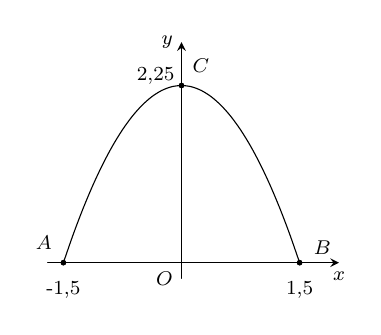
\begin{tikzpicture}[font=\footnotesize, line join=round, line cap=round, >=stealth, scale=1]
\path (-1.5,0) coordinate (A) (1.5,0) coordinate (B) (0,2.25) coordinate (C);
\draw[->] (-1.7,0)--(0,0)node[below left]{$O$}--(2,0)node[below]{$x$};
\draw[->] (0,-0.2)--(0,2.8)node[left]{$y$};
\draw[smooth] plot [domain=-1.5:1.5] (\x,{-(\x)^2+2.25});
\foreach \x/\n/\g in {A/A/135, A/{$-1{,}5$}/-90, B/B/34, B/{$1{,}5$}/-90, C/C/45, C/{$2{,}25$}/160}{
\fill (\x) circle (1pt)+(\g:0.35)node{$\n$};
}
\end{tikzpicture}}
\noindent
Khi đó tạo độ các điểm $A$, $B$, $C$ thỏa phương trình của $(P)$, ta có hệ phương trình
\[\heva{&a(-1{,})^2+b(-1{,}5)+c=0\\&a\cdot1^2+b\cdot1+c=0\\&a\cdot0+b\cdot0+c=2{,}25} \Leftrightarrow \heva{&a=-1\\&b=0\\&c=2{,}25.}\]
Suy ra $(P)\colon y=-x^2+2{,}25$.\\
Diện tích của của là $\displaystyle\int\limits_{-1{,}5}^{1{,}5}\left(-x^2+2{,}25\right)\mathrm{d}x=4{,}5$ (m$^2$).\\
Số tiền nhà trường phải trả là $4{,}5\cdot1{,}5=6{,}75$ (triệu đồng).
}
\end{ex}

\begin{ex}%[2D4H3-1]%[TEX Đề Moon 2025]%[Vũ Hồng Toàn]
\immini[thm]
{
Cho đồ thị $(C)$ của hàm đa thức bậc ba và parabol $(P)$ có trục đối xứng vuông góc với trục hoành như hình vẽ bên. Biết phần hình phẳng giới hạn bởi $(C)$ và $(P)$ (phần tô đậm của hình vẽ) có diện tích bằng $\dfrac{m}{n}$ ($m$, $n\in \mathbb{N}$; $\dfrac{m}{n}$ là phân số tối giản). Tính $m+n$.
}
{
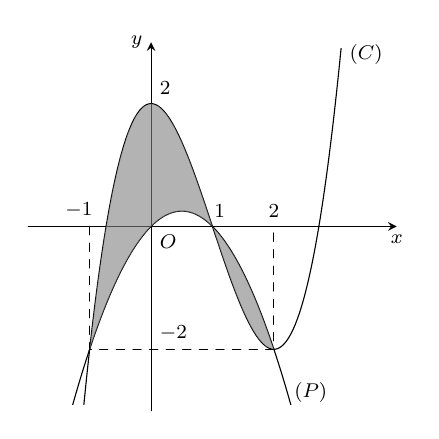
\begin{tikzpicture}[scale=0.78,>=stealth, font=\footnotesize, line join=round, line cap=round]
\def\xmin{-2} \def\xmax{4}
\def\ymin{-3} \def\ymax{3}
\draw[->] (\xmin,0)--(\xmax,0) node [below]{$x$};
\draw[->] (0,\ymin)--(0,\ymax) node [left]{$y$};
\node at (0,0) [below right]{$O$};
\draw[dashed] (-1,0)node[above,xshift=-0.15cm]{$-1$}--(-1,-2)--(0,-2)node[above right]{$-2$}--(2,-2)--(2,0)node[above]{$2$} (1,0)node[above,xshift=0.1cm]{$1$} (0,2)node[above right]{$2$} (2.6,-2.7)node[]{$(P)$} (3.5,2.8)node[]{$(C)$};
\clip (\xmin+0.1,\ymin+0.1) rectangle (\xmax-0.5,\ymax-0.1);
\draw[smooth,samples=300] plot(\x,{-(\x)^2+(\x)});
\draw[smooth,samples=300] plot(\x,{(\x)^3-3*(\x)^2+2});
\fill[gray,opacity=0.6] plot[domain=-1:2](\x,{-(\x)^2+(\x)})--plot[domain=2:-1](\x,{(\x)^3-3*(\x)^2+2})--cycle;
\end{tikzpicture}
}
\shortans{$49$}
\loigiai{
Gọi $A(-1;-2)$, $B(1;0)$, $C(2;-2)$,$D(0;2)$.\\
Giả sử $(C)$ có phương trình $f(x)=a x^3+bx^2+cx+d, a\ne0$ và $(P)$ có phương trình $g(x)= a_1x^2+b_1x+c_1, a_1\ne 0$.\\
Vì $A,B,C,D\in f(x)$ nên ta có hệ phương trình
\[\heva{&-a+b-c+d=-2\\&a+b+c+d=0\\&8a+4b+2c+d=-2\\&d=2}\Leftrightarrow\heva{&a=1\\&b=-3\\&c=0\\&d=2.}\]
Do đó $f(x)=x^3-3x^2+2$.\\
Tương tự ta cũng có $A,B,C\in g(x)$ nên ta có hệ phương trình
\[\heva{&a_1-b_1+c_1=-2\\&a_1+b_1+c_1=0\\&4a_1+2b_1+c_1=-2}\Leftrightarrow\heva{&a_1=-1\\&b_1=1\\&c_1=0.}\]
Do đó $g(x)=-x^2+x$.
Khi đó diện tích phần tô đậm trong hình vẽ là
\allowdisplaybreaks
\begin{eqnarray*}
S=\int\limits_{-1}^2\big|f(x)-g(x)\big|\mathrm{d}x&=&\int\limits_{-1}^2\big|x^3-2x^2-x+2\big|\mathrm{d}x\\
&=&	\int\limits_{-1}^1\big|x^3-2x^2-x+2\big|\mathrm{d}x+\int\limits_{1}^2\big|x^3-2x^2-x+2\big|\mathrm{d}x\\
&=&\left|\int\limits_{-1}^1\big(x^3-2x^2-x+2\big)\mathrm{d}x\right|+\left|\int\limits_{1}^2\big(x^3-2x^2-x+2\big)\mathrm{d}x\right|\\
&=&\left|\dfrac{8}{3}\right|+\left|\dfrac{5}{12}\right|=\dfrac{37}{12}.
\end{eqnarray*}
Suy ra $m=37$, $n=12$. Vậy $m+n=49$.
}
\end{ex}

\begin{ex}%[2D1H5-8]%[TEX ĐỀ MOON 2025]%[Nguyễn Văn Hiệp]
Một công ty sản xuất dụng cụ thể thao nhận được một đơn đặt hàng sản xuất $8\,000$ quả bóng tennis. Công ty này sở hữu một số máy móc, mỗi máy có thể sản xuất $30$ quả bóng trong một giờ. Chi phí thiết lập các máy này là $200$ nghìn đồng cho mỗi máy. Khi được thiết lập, hoạt động sản xuất sẽ hoàn toàn diễn ra tự động dưới sự giám sát. Số tiền phải trả cho người giám sát là $192$ nghìn đồng một giờ. Số máy móc công ty nên sử dụng là bao nhiêu để chi phí hoạt động là thấp nhất?
\shortans{$16$}
\loigiai{
\textbf{Bước 1: Thiết lập hàm chi phí} \\
Gọi $x$ là số máy ($x>0$, $x\in \mathbb{N}^*$), thời gian sản xuất
$t = \dfrac{8\,000}{30x}$ (giờ).\\
Chi phí
\[
C(x) = 200x + 192 \times \dfrac{8\,000}{30x}.
\]
\textbf{Bước 2: Tìm cực tiểu} \\
Ta có
\[
C'(x) = 200 - \dfrac{51200}{x^2} = 0 \Rightarrow x = 16.
\]
Bảng biến thiên
\begin{center}

\begin{tikzpicture}
\tkzTabInit[espcl=3.5,lgt=2.5,deltacl=1]
{$x$/0.7,$C'(x)$/1,$C(x)$/3}
{$0$,$16$,$+\infty$}
\tkzTabLine{,-,0,+,}
\tkzTabVar{+/$+\infty$,-/$C\left(16\right)$,+/$+\infty$}
\end{tikzpicture}
\end{center}
Vậy để chi phí hoạt động là thấp nhất, số máy móc công ty nên sử dụng là $16$ máy.
}
\end{ex}

\begin{ex}%[2D1H3-6]%[TEX ĐỀ MOON 2025]%[Lê Hữu Kiệt]
Trận bóng đá giao hữu giữa đội tuyển Việt Nam và Thái Lan ở sân vận động Mỹ Đình có sức chứa $55\,000$ khán giả. Ban tổ chức bán vé với giá mỗi vé là $100$ nghìn đồng, số khán giả trung bình đến sân xem bóng đá là $27\,000$ người. Qua thăm dò dư luận, người ta thấy rằng mỗi khi giá vé giảm thêm $10$ nghìn đồng, sẽ có thêm khoảng $3\,000$ khán giả. Hỏi ban tổ chức nên đặt giá vé là bao nhiêu để doanh thu từ tiền bán vé là lớn nhất với đơn vị tính giá vé là nghìn đồng?
\shortans{$95$}
\loigiai{Goi $x$ là số lần giảm $10$ nghìn đồng ($0\leq x\leq10$).\\
Khi đó, số tiền mỗi vé là  $100-10x$ (nghìn đồng), số khán giả là $27\,000+3\,000x$.\\
Doanh thu từ việc bán vé là $T(x)=(100-10x)(27\,000+3\,000x)=-30\,000x^2+30\,000x+2\,700\,000$.\\
Ta có $T'(x)=-60\,000x+30\,000$. Khi đó $T'(x)=0\Leftrightarrow x=0{,}5$.\\
Bảng biến thiên của $T(x)$ trên đoạn $[0;10]$ là
\begin{center}

\begin{tikzpicture}[font=\footnotesize, line join=round, line cap=round, >=stealth, scale=1]
\tkzTabInit[espcl=4,lgt=1.5,deltacl=1]
{$x$/0.7,$T'(x)$/0.7,$T(x)$/2}
{$0$, $0{,}5$, $10$}
\tkzTabLine{,+,$0$,-,}
\tkzTabVar{-/$2\,700\,000$, +/$2\,707\,500$, -/$0$}
\end{tikzpicture}
\end{center}
Từ bảng biến thiên suy ra hàm số $T(x)$ đạt giá trị lớn nhất khi $x=0{,}5$.\\
Vậy giá vé ban tổ chức nên đặt là $100-10\cdot0{,}5=95$ (nghìn đồng).
}
\end{ex}

\begin{ex}%[2D1H2-7]%[TEX ĐỀ MOON 2025]%[Nguyễn Cường]
Độ giảm huyết áp của một bệnh nhân được xác định bởi công thức $G(x)=0{,}024x^2(30-x)$, trong đó $x$ là liều lượng thuốc tiêm cho bệnh nhân cao huyết áp ($x$ được tính bằng mg). Tìm lượng thuốc để tiêm cho bệnh nhân cao huyết áp để huyết áp giảm nhiều nhất.
\shortans{$20$}
\loigiai
{
Ta có $G(x)=-0{,}024x^3+0{,}72x^2$ với $0\le x\le 30$.\\
Đạo hàm $G'(x)=-0{,}072x^2+1{,}44x$.\\
Xét $G'(x)=0\Leftrightarrow -0{,}072x^2+1{,}44x=0\Leftrightarrow\hoac{&x=0\\&x=20.}$\\
Lúc này $G(0)=G(30)=0$ và $G(20)=96$.\\
Vậy lượng thuốc tiêm cho bệnh nhân cao huyết áp để giảm huyết áp nhiều nhất là $20$\,(mg).
}
\end{ex}

\begin{ex}%[2H2H2-6]
Một chiếc máy bay không người lái bay lên tại một điểm. Sau một thời gian bay, chiếc máy bay cách điểm xuất phát về phía Bắc $50$ (km) và về phía Tây $20$ (km), đồng thời cách mặt đất $1$ (km). Xác định khoảng cách của chiếc máy bay với vị trí tại điểm xuất phát của nó (làm tròn kết quả đến hàng phần mười).
\shortans{53{,}9}
\loigiai{
Chọn hệ trục tọa độ $Oxyz$ với gốc $O$ là điểm xuất phát, trục $Ox$ hướng về phía Bắc, trục $Oy$ hướng về phía Tây, trục $Oz$ hướng lên trên.\\
Tọa độ của máy bay là $\mathrm{P}\left(-20;50;1\right)$.\\
Khoảng cách từ máy bay đến điểm xuất phát $O(0;0;0)$ là
$OP=\sqrt{(-20)^2+50^2+1^2} \approx 53{,}9$ (km).
}
\end{ex}

% \paragraph{Mức độ V}
\begin{ex}%[1H8V7-9]%[TEX ĐỀ MOON 2025]%[Huỳnh Thanh Chí]
Người ta cần trang trí một kim tự tháp hình chóp tứ giác đều $S.ABCD$ có cạnh bên bằng $200$ m, góc $\widehat{ASB}=15^\circ$ bằng đường gấp khúc dây đèn led vong quanh kim tự tháp $AEFGHIJKLS$. Trong đó điểm $L$ cố định và $LS=40$ m.
\begin{center}
\begin{tikzpicture}[scale=1,>=stealth, font=\footnotesize, line join=round, line cap=round]
\coordinate (A) at (-1.9,-1.6);
\coordinate (B) at (0,0);
\coordinate (D) at (1.6,-1.6);
\coordinate (C) at ($(B)+(D)-(A)$);
\coordinate (O) at ($(A)!1/2!(C)$);
\coordinate (S) at ($(O)+(0,4)$);
\coordinate (L) at ($(S)!0.2!(A)$);
\coordinate (K) at ($(S)!0.28!(D)$);
\coordinate (J) at ($(S)!0.4!(C)$);
\coordinate (I) at ($(S)!0.65!(B)$);
\coordinate (H) at ($(S)!0.45!(A)$);
\coordinate (G) at ($(S)!0.55!(D)$);
\coordinate (F) at ($(S)!0.7!(C)$);
\coordinate (E) at ($(S)!0.8!(B)$);
\draw (S)--(A)--(D)--(C)--cycle (S)--(D) (F)--(G)--(H) (J)--(K)--(L);
\draw[dashed] (A)--(B)--(C) (S)--(B) (A)--(E)--(F) (H)--(I)--(J);
\foreach \x/\g in {S/90,A/-150,B/-60,C/0,D/-45,E/170,F/45,G/-30,H/170,I/140,J/30,K/60,L/170}
\fill[black] (\x) circle (1pt) ($(\g:3mm)+(\x)$) node {$\x$};
\end{tikzpicture}
\end{center}
Hỏi khi đó cần dùng ít nhất bao nhiêu mét dây đèn led để trăng trí? (làm tròn đến hàng đơn vị).

\shortans[]{$263$}
\loigiai{
Ta trải hình chóp tứ giác đều thành vẽ như sau
\begin{center}
\begin{tikzpicture}[scale=1.5,font=\footnotesize,line join=round,line cap=round,>=stealth]
\def\a{4}
\def\r{15}
\path
(0,0) coordinate (S)
(-135:\a) coordinate (A)
(-135+\r:\a) coordinate (D)
($(A)!1!-90:(D)$) coordinate (B_2)
($(D)!1!90:(A)$) coordinate (C_2)
;
\foreach \x/\i in {C/2,B/3,A_1/4,D_1/5,C_1/6,B_1/7,A_2/8}{
\path
(-135+\i*\r:\a) coordinate (\x)
;
\draw (S)--(\x);
}
\foreach \x/\y/\i in {A/L/1,D/K/2,C/J/3,B/I/4,A_1/H/5,D_1/G/6,C_1/F/7,B_1/E/8,
A_1/H_1/7,B/I_1/6,C/J_1/5,D/K_1/4
}{
\path
($(S)!1/9*\i!(\x)$) coordinate (\y)
;}
\draw (S)--(D)--(C_2)--(B_2)--(A)--(S) (A)--(D)--(C)--(B)--(A_1)--(D_1)--(C_1)--(B_1)--(A_2)
(L)--(K)--(J)--(I)--(H)--(G)--(F)--(E)--(A_2)--(L)
%	(K1)--(J1)--(I1)--(H1)
;

\foreach \x/\g in {A/135,D/-65,S/180,C/-90,B/-90,A_1/-90,D_1/-90,C_1/-60,B_1/-45,A_2/0,C_2/-135,B_2/-90}
\fill 	(\x) circle (1pt)
($(\g:3mm)+(\x)$) node {$\x$};
\foreach \x/\g in {L/135,K/-90,J/-90,I/-90,H/-90,G/-90,F/-90,E/-90}
\fill 	(\x) circle (1pt)
($(\g:3mm)+(\x)$) node {$\x$};
\end{tikzpicture}
\end{center}
Ta có $T=SL+LK+KJ+\ldots+EA_2\ge SL+LA_2$ (vì $SL$ không đổi).\\
Để sợi dây trang trí ngắn nhất thì $T=SL+LA_2$.\\
Ta có $\widehat{LSA_2}=15^\circ \cdot 8=120^\circ$.\\
Áp dụng định lí cosin vào $\triangle SLA_2$ có
\allowdisplaybreaks
\begin{eqnarray*}
LA_2=\sqrt{SL^2+SA_2^2-2\cdot SL\cdot SA_2\cdot\cos \widehat{SLA_2}}=40\sqrt{31}.
\end{eqnarray*}
Vậy $T=40+40\sqrt{31}\approx 263$.
}
\end{ex}

\begin{ex}%[1H8V7-4]%[TEX Đề Moon 2025]%[Vũ Hồng Toàn]
Cho hình lăng trụ $ABC.A'B'C'$ có đáy $ABC$ là tam giác đều cạnh bằng $\sqrt{3}$. Hình chiếu vuông góc của $A'$ lên mặt phẳng $(ABC)$ trùng với trọng tâm tam giác $ABC$. Biết khoảng cách giữa hai đường thẳng $AA'$ và $BC$ bằng $\dfrac{3}{4}$. Tính thể tích $V$ của khối lăng trụ $ABC.A'B'C'$ (kết quả làm tròn đến hàng phần trăm).
\shortans{$0{,}75$}
\loigiai{
\begin{center}
\begin{tikzpicture}[scale=1, line join = round, line cap=round,>=stealth,font=\footnotesize,declare function={a=4; b=0.54*a; h=3.5;goc=-50;}]
\path
(0,0) coordinate (A)
(a,0) coordinate (C)
(goc:b) coordinate (B)
($(B)!.5!(C)$)coordinate (M)
($(A)!2/3!(M)$)coordinate (G)++(0,h)coordinate (A')
($(A')+(a,0)$)coordinate (C')
($(A')+(goc:b)$)coordinate (B')
($(A)!(G)!(A')$)coordinate (H)
($(A)!(M)!(A')$)coordinate (I)
;
\draw[dashed] (M)--(A)--(C) (M)--(A')--(G) (G)--(H) (M)--(I);
\draw (A')--(B')--(C')--cycle (A')--(A)--(B)--(B') (M)--(B)--(C)--(C');
\foreach \x/\goc in {A/220,B/-40,C/0,G/-120,A'/180,B'/70,C'/0,M/-30,H/180,I/130}{
\draw[fill] (\x) circle (1pt) node[shift={(\goc:7pt)},font=\small]{$\x$};
}
\end{tikzpicture}
\end{center}
Gọi $G$ là trọng tâm tam giác $ABC$ và $M$ là trung điểm của $BC$.\\
Ta có $A'G \perp(ABC)$ nên $A'G \perp BC$; $BC \perp AM \Rightarrow BC \perp\left(MAA'\right)$.\\
Kẻ $MI \perp AA'$; $BC \perp IM$ nên $\mathrm{d}\left(AA', BC\right)=I M=\dfrac{3}{4}$.\\

Kẻ $GH \perp AA'$, ta có
\begin{itemize}
\item $\dfrac{A G}{A M}=\dfrac{G H}{I M}=\frac{2}{3} \Leftrightarrow G H=\dfrac{AG}{AM}\cdot IM=\dfrac{2}{3} \cdot \dfrac{3}{4}=\dfrac{1}{2}$.
\item $AM=\dfrac{AB\sqrt{3}}{2}=\dfrac{3}{2}$; $AG=\dfrac{2}{3}AM=\dfrac{2}{3}\cdot\dfrac{3}{2}=1$;
\item $\dfrac{1}{H G^2}=\dfrac{1}{A'G^2}+\dfrac{1}{A G^2} \Leftrightarrow A'G=\dfrac{AG \cdot HG}{\sqrt{AG^2-H G^2}}=\dfrac{1 \cdot \dfrac{1}{2}}{\sqrt{1-\left(\dfrac{1}{2}\right)^2}}=\dfrac{\sqrt{3}}{3}$.
\end{itemize}
Vậy $V_{ABC.A'B'C'}=A'G \cdot S_{A B C}=\dfrac{\sqrt{3}}{3} \cdot \dfrac{3 \sqrt{3}}{4}=\dfrac{3}{4}=0{,}75$.
}
\end{ex}

\begin{ex}%[1H8V7-3]
Cho hình chóp $S.ABCD$ có đáy $ABCD$ là hình vuông cạnh $2$, tam giác $SAB$ vuông cân tại và nằm trong mặt phẳng vuông góc với đáy. Gọi $(P)$ là mặt phẳng chứa $CD$ và vuông góc với $(ABCD)$. Trên $(P)$ lấy điểm $M$ bất kỳ, thể tích khối tứ diện $SAMB$ bằng bao nhiêu? \textit{(làm tròn kết quả đến hàng phần trăm)}.
\shortans{$0{,}67$}
\loigiai{
\begin{center}
\begin{tikzpicture}[scale=1, font=\footnotesize,>=stealth]
%Gán số liệu.
\def\canhAD{4};\def\canhBA{2};\def\gocBAD{-130};\def\h{3};\def\xdinhS{-1};
%Gán tọa độ.
\coordinate (A) at (0,0);
\coordinate (B) at ($(A)+(\gocBAD:\canhBA)$);
\coordinate (C) at ($(B)+(0:\canhAD)$);
\coordinate (D) at ($(A)+(0:\canhAD)$);
\coordinate (S) at ($(A)+(\xdinhS,\h)$);
\coordinate (O) at (intersection of A--C and B--D);
\coordinate (H) at ($(A)!0.5!(B)$);
\coordinate (M) at ($(C)!0.5!(D)$);
\coordinate (a) at ($(S)+(C)-(B)$);
\coordinate (b) at ($(a)+(D)-(C)$);
%Vẽ khối chóp S.ABCD.
\draw (B)--(S)--(C)--cycle (D)--(C) (C)--(a)--(b)--(D);
\draw[dashed] (A)--(D) (A)--(C) (B)--(D) (S)--(A)--(B) (S)--(H) (S)--(D);
\draw pic[draw, angle radius=3mm, angle eccentricity=1.5]{right angle = S--H--A};
\draw pic[draw, angle radius=10mm, angle eccentricity=1.5]{ angle = a--b--D};
\draw($(b)-(0.3,0.7)$) node {P};
%Gán nhãn.
\foreach \x/\y in {A/180,B/-90,C/-90,D/0,S/90,O/225, H/-90, M/0}{\fill (\x) circle(1pt) ($(\x)+(\y:0.3cm)$) node{$\x$};}
\end{tikzpicture}
\end{center}
Gọi $H$ là trung điểm $AB$, vì tam giác $SAB$ vuông cân tại $S$ nên $SH\perp AB$ và $SH=\dfrac{AB}{2}=a$.\\
Suy ra diện tích tam giác $SAB$ là $S_{ABS}=\dfrac{AB\cdot SH}{2}=\dfrac{2}{2}=1$.\\
Vì $(SAB)\perp(ABCD)$, lại có $SH\perp AB$ nên $SH\perp(ABCD)$.\\
Mặt khác $(SAB)\perp(ABCD)$ và $(P)\perp(ABCD)$ nên $(P)\parallel(SAB)$.\\
Lấy điểm $M$ trên $CD$, vì $CD\parallel(SAB)$ nên $\mathrm{d}(M;(SAB))=\mathrm{d}(C;(SAB))$.\\
Ta có $CB\perp AB$, $CB\perp SH$ nên $CB\perp(SAB)$ hay $\mathrm{d}(C,(SAB))=BC=2\Rightarrow \mathrm{d}(M,(SAB))=2$.\\
Vậy thể tích khối tứ diện $SAMB$ là $V_{SAMB}=\dfrac{1}{3} \mathrm{d}(M,(SAB))\cdot S_{ABS}=\dfrac{1}{3}\cdot 2\cdot 1=\dfrac{2}{3}$.
}
\end{ex}

\begin{ex}%[1H8V7-3]
Cho tứ diện $ABCD$, tam giác $ABC$ vuông cân tại $B$, $DA$ vuông góc với mặt phẳng $(ABC)$, $M$ là trung điểm $AC$, $AB=2$, góc giữa đường thẳng $CD$ với mặt phẳng $(BDM)$ bằng $\alpha$ biết $\sin\alpha=\dfrac{1}{3}$. Thể tích của khối tứ diện $ABCD$ bằng bao nhiêu? (làm tròn kết quả đến hàng phần mười).
\shortans{$1{,}3$}
\loigiai{
\begin{center}


\begin{tikzpicture}[scale=1]
\def\a{4}
\def\h{4}
\path 	(0:0) coordinate (A)
++(0:\a) coordinate (B)
++(-130:4*\a/5) coordinate (C)
($(A)+(90:\h)$) coordinate (D)
($(A)!0.5!(C)$) coordinate (M)
($(D)!(A)!(M)$) coordinate (H)
;
\draw[thick] 	(A)--(C)--(B)
(A)--(D)	(B)--(D)	(C)--(D)--(M) (A)--(H);
\draw[dashed,thick] 	(A)--(B);
\foreach \x /\goc in {A/180,B/0,C/-135,D/90,M/-110,H/150}
\fill[black] (\x) circle (1.5pt)
($(\x)+(\goc:3mm)$) node {$\x$};
\draw pic[draw,angle radius=2mm]{right angle=B--A--D};
\draw pic[draw,angle radius=2mm]{right angle=A--H--M};
\end{tikzpicture}

\end{center}
Tam giác $ABC$ vuông cân tại $B$ có $AB=2 \Rightarrow S_{A B C}=\dfrac{1}{2} \cdot A B \cdot B C=\dfrac{1}{2} \cdot 2 \cdot 2=2$.\\
Kẻ $A H \perp M D$, ta có
$B M \perp A H( \text{ do } B M \perp(D A C)) \Rightarrow AH \perp (BDM)$.\\
Ta có
\begin{align*}
\sin \alpha=\dfrac{\mathrm{d}(C,(B D M))}{C D}
=\dfrac{\mathrm{d}(A,(B D M))}{C D}  =\dfrac{A H}{C D}=\dfrac{1}{3} \tag{1}
\end{align*}
Lại có
\begin{align*}
A H=\dfrac{A D \cdot A M}{\sqrt{A D^2+A M^2}} =\dfrac{A D \cdot \sqrt{2}}{\sqrt{A D^2+(\sqrt{2})^2}};
C D=\sqrt{A D^2+A C^2} =\sqrt{A D^2+8}  \tag{2}
\end{align*}
Từ (1) và (2) suy ra $AD=2$. Khi đó thể tích của khối tứ diện $ABCD$ là
\[ V_{A B C D}=\dfrac{1}{3} \cdot A D \cdot S_{A B C}=\dfrac{1}{3} \cdot 2 \cdot 2  =\dfrac{4}{3} \approx 1{,}3 .\]
}
\end{ex}

\begin{ex}%[1H8V7-3]
Cho khối trụ có trục $OO'=6$. Một khối chóp đều $O.ABCD$ có thể tích bằng $16$ và đáy $ABCD$ nội tiếp đường tròn $(O')$ là đường tròn đáy của khối trụ. Thể tích của khối trụ đã cho là $k\pi$, giá trị của $k$ bằng bao nhiêu?
\shortans[]{$24$}
\loigiai{
\begin{center}
\begin{tikzpicture}[font=\footnotesize,line join=round, line cap=round, >=stealth,scale=0.3]
\path
(0,0) coordinate (A)
(-7.5,-4) coordinate (D)
(7.5,-4) coordinate (C)
(15,0) coordinate (B)
(3.5,10.5) coordinate (O)
($(A)!0.5!(C)$) coordinate (O')
;
\draw (O)--(C) (O)--(D) (B)--(O)--(D)--(C)--(B);
\draw[dashed] (O')--(O)--(A)--(B)--(D)--(A)--(C);
\foreach \x/\pos in{A/180,D/-150,C/-30,B/60,O/50, O'/-100}
\fill (\x) circle(1pt) node[{shift=(\pos:0.25)}]{$\x$};
\end{tikzpicture}
\end{center}
Ta có $V_{O.ABCD}=\dfrac{1}{3}OO'\cdot S_{ABCD}=16\Rightarrow S_{ABCD}=8$. Vì $ABCD$ là hình vuông nên $AB=\sqrt{8}=2\sqrt{2}$.
Ta có khối trụ có bán kính đáy bằng bán kính đường tròn $(O')$ và bằng $\dfrac{1}{2}$ độ dài đường chéo của hình vuông $ABCD$ và bằng $2$.\\ Suy ra thể tích của khối trụ bằng
\[OO'\cdot\pi r^2=6\cdot 2^2\pi=24\pi.\]
Vậy $k=24$.
}
\end{ex}

\begin{ex}%[1H8V6-2]
Cho hình lập phương $ABCD.A'B'C'D'$. Số đo của góc nhị diện $\left[B',A'C,D' \right]$ bằng bao nhiêu độ?
\shortans{120}
\loigiai{
\begin{center}
\begin{tikzpicture}[scale=0.6, font=\footnotesize,line join=round, line cap=round, >=stealth]
\path
(0,0) coordinate (A)
++(-130:3) coordinate (B)
++(0:4) coordinate (C)
($(A)+(C)-(B)$) coordinate (D)
($(A')!0.3!(C)$) coordinate (H)
;
\foreach \i in {A,B,C,D}{
\coordinate (\i') at ($(\i)+(0,4)$);
}
\draw (A')--(B')--(C')--(D')--cycle;
\draw (B)--(B') (C)--(C') (D)--(D')  (B)--(C)--(D) (A')--(C') (B')--(D');
\draw[dashed,thin](B)--(A)--(A')--(C) (A)--(D) (B')--(C)--(D') (D')--(H)--(B');
\draw (A')--(C') node[midway,above right]{$O$};
\foreach \i/\g in {A'/90,B'/90,C'/90,D'/90,A/-90,B/-90,C/-90,D/-90,H/-20}
\fill[black] (\i) circle(1pt)+(\g:5mm)node[scale=1]{$\i$};
\end{tikzpicture}
\end{center}
Ta có $\heva{&A'C'\perp B'O\\&AA'\perp B'O\\&AA',A'C'\in \left( AA'CC'\right) }$ suy ra $B'O\perp\left(AA'CC'\right)\Rightarrow B'O\perp A'C$.\\
Lại có $OH\perp A'C\Rightarrow A'C\perp \left(B'OH \right)\Rightarrow A'C\perp B'H$.\\
Tương tự ta chứng minh $A'C\perp D'H$.\\
Suy ra góc nhị diện $\left[B',A'C,D' \right]$ là góc $\widehat{B'HD'}$.\\
Cho các cạnh hình lập phương là $a$.\\
Ta có $B'D'=a\sqrt{2}$.\\
Xét tam giác $A'B'C$ vuông tại $B'$ ta có
\[\dfrac{1}{B'H^2}=\dfrac{1}{A'B'^2}+\dfrac{1}{B'C^2}=\dfrac{1}{a^2}+\dfrac{1}{2a^2}=\dfrac{3}{2a^2}.\]
Suy ra $B'H=a\sqrt{\dfrac{2}{3}}$.\\
Tương tự $D'H=a\sqrt{\dfrac{2}{3}}$.\\
Ta có $\cos \widehat{B'HD'}=\dfrac{B'H^2+HD'^2-B'D'^2}{2\cdot B'H\cdot HD'}\Rightarrow \widehat{B'HD'}=120^\circ$.\\
Vậy số đo của góc nhị diện $\left[B',A'C,D' \right]$ bằng $120^\circ$.
}
\end{ex}

\begin{ex}%[1H8V5-4]%[Tex đề Moon 2025]%[Nguyễn Hồng Thạch]
Cho hình chóp $S.ABC$ có đáy $ABC$ là tam giác vuông cân tại $A$, tam giác $SBC$ là tam giác đều cạnh $1$ và thuộc mặt phẳng vuông góc với đáy. Tính khoảng cách giữa hai đường thẳng $SA$ và $BC$ (làm tròn kết quả đến hàng phần trăm).
\shortans{$0{,}43$}
\loigiai{
\begin{center}
\begin{tikzpicture}
\def\a{4}
\def\h{4}
\path 	(0:0) coordinate (A)
++(0:\a) coordinate (B)
++(-150:4*\a/5) coordinate (C)
($(C)!1/2!(B)$) coordinate (I)
($(I)+(90:\h)$) coordinate (S)
($(S)!2/3!(A)$) coordinate (H);
\draw (C)--(A) (C)--(B)
(A)--(S)	(B)--(S)	(C)--(S) (S)--(I);
\draw[dashed] (A)--(B) (A)--(I) (I)--(H);
\foreach \x / \goc in 		{A/180,B/0,C/-135,I/-45,S/90,H/135}
\fill (\x) circle (1.5pt)
($(\x)+(\goc:3mm)$) node {$\x$};

\draw pic[draw,angle radius=2mm]{right angle=A--I--S};
\draw pic[draw,angle radius=2mm]{right angle=A--H--I};%Theo chiều dương
\end{tikzpicture}
\end{center}
Gọi $I$ là trung điểm $BC$.\\
Ta có $\triangle SBC$ đều nên $SI\perp BC$.\\
Vì $\heva{&BC=(SBC)\cap (ABC)\\
&SI\subset (SBC)\\&SI\perp BC}$ nên $SI\perp (ABC)$.\\
Suy ra $SI\perp AI$ hay tam giác $SAI$ vuông tại $I$.\\
Từ $I$ kẻ $IH$ vuông góc với $SA$.\\
Ta có $\heva{&BC\perp SI\\&BC\perp AI}\Rightarrow BC\perp (SAI)\Rightarrow BC\perp IH$.\\
Khi đó ta có $IH$ là đoạn vuông góc chung của $SA$ và $BC$.\\
Trong tam giác $SAI$ có $AI=\dfrac{BC}{2}=\dfrac{1}{2}$,\quad $SI=\dfrac{\sqrt{3}}{2}$.\\
$\Rightarrow \dfrac{1}{IH^2}=\dfrac{1}{SI^2}+\dfrac{1}{AI^2}=\dfrac{1}{\left(\dfrac{\sqrt{3}}{2}\right)^2}+\dfrac{1}{\left(\dfrac{1}{2}\right)^2}=\dfrac{16}{3}$.\\
Vậy $\mathrm{d}(SA,BC)=IH=\dfrac{\sqrt{3}}{4}\approx 0{,}43$.
}
\end{ex}

\begin{ex}%[1H8V5-4]%[TEX Đề Moon 2025]%[Võ Nguyên Thạch]
Cho hình chóp $S.ABCD$ có $SA\perp(ABCD)$, đáy $ABCD$ là hình chữ nhật và $AD=6$. Góc giữa cạnh bên $SD$ và mặt đáy bằng $30^\circ$. Khoảng cách giữa hai đường thẳng $AB$ và $SD$ bằng bao nhiêu?
\shortans{3}
\loigiai{
\begin{center}
\begin{tikzpicture}
\def\a{4}
\def\h{4}
\path 	(0:0) coordinate (A)
++(0:\a) coordinate (D)
++(-130:\a/2) coordinate (C)
($(A)+(C)-(D)$) coordinate (B)
($(A)+(90:\h)$) coordinate (S)
(intersection of A--C and B--D) coordinate (O)%giao điểm O
($(S)!(A)!(D)$) coordinate (H);
\draw[dashed,thick] 	(B)--(A)--(D)	(A)--(S) (A)--(H);
\draw[thick] 			(B)-- (C)--(D)
(B)--(S)	(C)--(S)	(D)--(S);
\foreach \x/\g in {A/135,B/-135,C/-45,D/45,S/90,H/45}
\fill[black] 	(\x) circle (1.5pt)
($(\g:3mm)+(\x)$) node {$\x$};
\draw pic["$30^\circ$",draw,angle eccentricity=1.8,angle radius=0.5cm]{angle=S--D--A};
\draw pic[draw,angle radius=3mm]{right angle=D--A--S};%Theo chiều dương
\end{tikzpicture}
\end{center}
Trong mặt phẳng $(SAD)$, kẻ $AH\perp SD=H$.\\
Ta có $\heva{&SA\perp (ABCD)\Rightarrow AH\perp AB\\&AD\perp AB.}$\\
Suy ra $AB\perp (SAD)$, mà $AH\subset (SAD)$ nên $AB\perp AH$.\\
Khi đó, $AH$ là đoạn vuông góc chung của $AB$ và $SD$.\\
Xét tam giác $SAD$ vuông tại $A$, có
\[\tan \widehat{SDA}=\dfrac{SA}{AD}\Leftrightarrow SA=AD\tan \widehat{SDA}=6\tan 30^\circ = 2\sqrt 3.\]
Xét tam giác $SAD$ vuông tại $A$ có đường cao $AH$
\[\dfrac{1}{AH^2}+\dfrac{1}{SA^2}+\dfrac{1}{AD^2}\Leftrightarrow AH=\dfrac{SA\cdot AD}{\sqrt{SA^2+AD^2}}=\dfrac{2\sqrt 3\cdot 6}{\sqrt{(2\sqrt 3)^2+6^2}}=3.\]
}
\end{ex}

\begin{ex}%[1D6V4-6]
Chị Lan vừa mua một chiếc máy tính xách tay mới với giá $25$ triệu đồng vào ngày $20/9/2022$ bằng thẻ tín dụng của ngân hàng Y. Thẻ tín dụng này được phát hành vào ngày $10/9/2022$. Ngân hàng Y có chế độ không tính lãi trong $45$ ngày đầu và cộng thêm khuyến mãi $15$ ngày tiếp theo không tính lãi. Sau thời gian này, ngân hàng sẽ tính lãi với lāi suất $18\%$ /năm (tính lāi kép theo ngày). Chị Lan dự định sē hoàn tiền cho ngân hàng vào ngày $10/12/2022$. Chị Lan phải trả thêm bao nhiêu nghìn đồng tiền lāi so với giá gốc cho ngân hàng vào ngày $10/12/2022$? \textit{(kết quả làm tròn đến hàng đơn vị)}.
\shortans{$260$}
\loigiai{
Ngân hàng miễn lãi trong $45$ ngày đầu và $15$ ngày khuyến mãi $60$ ngày miễn lãi.\\
Thời gian tính lãi là từ ngày $20/11/2022$ đến ngày $10/12/2022$ nên số ngày có lãi là $21$ ngày.\\
Lãi suất hàng năm là $18\%/$ năm.\\
Suy ra lãi suất hàng ngày là $\dfrac{18}{365}$.\\
Số tiền chị Lan phải trả cho ngân hàng vào ngày $10/12/2022$ là
\[T=25\cdot \left(1+\dfrac{18}{365} \%\right)^{21} \approx 25{,}260 \text{ (triệu đồng)}.\]
Số tiền lãi chị Lan phải trả cho ngân hàng là $25 \,260\,000-25\,000\,000=260\,000$ (đồng).
}
\end{ex}

\begin{ex}%[1D6V3-5]%[TEX Đề Moon 2025]%[Vũ Hồng Toàn]
Một người vay ngân hàng số tiền $350$ triệu đồng, hàng tháng (tính từ ngày gửi) người đó trả góp $8$ triệu đồng. Lãi suất cho số tiền chưa trả là $0{,}79\%$ một tháng và kỳ trả đầu tiên là cuối tháng thứ nhất. Biết số tiền phải trả ở kỳ cuối là $m$ triệu đồng thì người đó trả hết nợ ngân hàng. Tính giá trị $m$ ($m$ làm tròn đến hàng phần trăm).
\shortans{$7{,}14$}
\loigiai{
Gọi $A$ là số tiền vay ngân hàng, $B$ là số tiền trả trong mỗi chu kì, $r=79 \%=0{,}0079$ là lãi suất cho số tiền chưa trả trên một chu kì, $n$ là số kì trả nợ.\\
Số tiền còn nợ ngàn hàng (tính cả lãi) trong từng chu kì như sau
\begin{itemize}
\item Đầu kì thứ nhất là $A$.
\item Cuối kì thứ nhất là $A(1+r)- B$.
\item Cuối kì thứ hai là
$[A(1+r)-n](1+r)-A=A(1+r)-A[(1+r)+1]$.
\item Cuối kì thứ ba là
\[\left[A(1+r)^2-B[(1+r)+1]\right]\left(1+r\right)-B=A(1+r)^3-B\left[(1+r)^2+(1+r)+1\right].\]
$\ldots$
\item Theo giả thiết quy nạp, cuối kì thứ $n$ là
\[A(1+r)^n-B\left[(1+r)^{n-1}+\cdots+(1+r)+1\right]=A(1+r)^n-B\cdot  \dfrac{(1+r)^n-1}{r}.\]
\end{itemize}
Vậy số tiền còn nợ (tính cả lãi) sau $n$ chu kì là
$A(1+r)^n-B\cdot \dfrac{(1+r)^n-1}{r}$.\\
Người đó trả hết nợ ngân hàng khi
\allowdisplaybreaks
\begin{eqnarray*}
&&A(1+r)^n-B\cdot \dfrac{(1+r)^n-1}{r}=0\\
&\Leftrightarrow&(1+r)^n=\dfrac{B}{B-Ar}\\
&\Leftrightarrow& n =\log_{(1+r)}\dfrac{B}{Ar-B}=\log_{1{,}0079}\dfrac{8}{350\cdot 0{,}0079-8}\approx 53{,}9.
\end{eqnarray*}
Tức là phải mất $54$ tháng người này mới trả hết nợ.\\
Cuối tháng thứ $53$, số tiền còn nợ (tính cả lãi) là
\[S_{53}=350\cdot 1{,}0079^{53}-8 \cdot \dfrac{1{,}0079^{53}-1}{0{,}0079} \text{(triệu đồng)}.\]
Kì trả nợ tiếp theo là cuối tháng thứ $54$, khi đó người vay phải trả số tiền
$S_{53}$ và lãi của số tiền này nữa là $S_{53}+0{,}0079 \cdot S_{53}=S_{53} \cdot 1{,}0079 \approx 7{,}14$ (triệu đồng).
}
\end{ex}

\begin{ex}%[1D2V2-7]
\immini[thm]
{
An đã tạo ra một cầu thang $3$ bậc bằng $18$ que tăm như hình minh họa. Vậy An cần thêm bao nhiêu que tăm để hoàn thành một cầu thang $5$ bậc?
}
{
\includegraphics[scale=0.16]{images/de15-1}
}
\shortans[]{$22$}
\loigiai{
\begin{itemize}
\item \textbf{Cách 1}\\
Ta thấy rằng cầu thang $1$ bậc cần $4$ tăm và cầu thang $2$ bậc cần $10$ tăm. Do đó, để đi từ cầu thang $1$ bậc đến $2$ bậc cần thêm $6$ tăm và để đi từ cầu thang $2$ bậc đến $3$ bậc cần thêm $8$ tăm.\\
Áp dụng mô hình này, để đi từ cầu thang $3$ bậc đến $4$ bậc cần thêm $10$ tăm và để đi từ cầu thang $4$ bậc đến $5$ bậc cần thêm $12$ tăm.\\
Vậy bạn An cần thêm $10+12=22$ tăm.
\item \textbf{Cách 2}\\
Với cầu thang $3$ bậc có $2\left[2\cdot 3+2+1\right]=18$ tăm.\\
Tổng quát, ta thấy rằng cầu thang có $x$ bậc có
\[2\left[2x+(x-1)+(x-2)+\ldots+1\right]\,\text{tăm}.\]
Vì vậy đối với $x=5$ bậc ta có
\[2\left[2\cdot 5+4+3+2+1\right]=40\,\text{tăm}.\]
Vậy bạn An cần thêm $40-18=22$ tăm.
\item \textbf{Cách 3}\\
Ta thấy rằng để đến được $4$ các bước, ta thêm hai khối có ba que (phía trên và bên phải) va fhai khối nữa có hai khối toạ thành các bước. Điều này sẽ có thêm $2\cdot 3+2\cdot 2=10$ quê. \\
Sau đó,để đếm được $5$ các bước, ta thêm hai khối cạnh nữa có $3$ que và $3$ nữa có hai que. Ta thêm $2\cdot 3+3\cdot 2=12$ nhiều hơn nữa để tăng tổng cộng $10+12=22$ que.
\end{itemize}
}
\end{ex}

\begin{ex}%[1D2V1-6]
\immini{Một chai soda có giá $1$ đô. Sau khi uống, hai chai rỗng sẽ được đổi lấy một chai soda. Bạn có thể uống nhiều nhất bao nhiêu chai soda nếu bạn có $100$ đô?}{\begin{tikzpicture}[very thick,>=stealth',scale=0.7]
\filldraw[black] (-0.25,3.8)--(-0.25,3.5) arc (180:360:0.25 and 0.1)--(0.25,3.8) arc (0:-180:0.25 and 0.1);
\filldraw[blue!70!green!30] (-0.6,0.5)--(-0.6,-2) arc (180:0:0.6 and 0.3)--(0.6,0.5);
\filldraw[blue!50!green!50,,] (0,0.5) ellipse (0.6 and 0.3);
\filldraw[blue!50!green!50] (0,-2) ellipse (0.6 and 0.3);
\draw (-0.6,1) -- (-0.6,-2) (0.6,1) -- (0.6,-2);
\draw (0,-2) ellipse (0.6 and 0.3);
\draw (-0.6,1)--(-0.6,1.5)--(-0.25,2.8)--(-0.25,3.8);
\draw (0.6,1)--(0.6,1.5)--(0.25,2.8)--(0.25,3.8);
\draw (0,3.8) ellipse (0.25 and 0.1);
\end{tikzpicture}}
\shortans{199}
\loigiai{
\textbf{Mua số lượng chai soda ban đầu:}\\
Với $100$ đô ta sẽ mua được $100$ chai soda.\\
Đổi chai rỗng lấy soda: Sau khi uống $100$ chai, ta sẽ có $100$ chai rỗng, $100$ chai rỗng ta sẽ đổi được 50
chai soda mới.\\
\textbf{	Tiếp tục quy trình:}\\
Sau khi uống $50$ chai soda mới, ta được $50$ chai rỗng.
Đổi $50$ chai rỗng lấy $25$ chai soda mới.\\
\textbf{Lặp lại quy trình:}\\
Uống $25$ chai so da mới, ta được $25$ chai rỗng.\\
Đổi $25$ chai rỗng ta được $12$ chai soda mới và dư $1$ chai rỗng.\\
\textbf{	Tiếp tục đổi:}\\
Uống $12$ chai soda mới ta sẽ có $12$ chai rỗng.\\
Đổi $12$ chai rỗng ta được $6$ chai so đa mới.\\
\textbf{Lặp lại quy trình:}\\
Uống $6$ chai so da mới, ta được $6$ chai rỗng.\\
Đổi $6$ chai rỗng ta được $3$ chai soda mới.\\
\textbf{Tiếp tục đổi:}\\
Uống chai $3$ soda mới vừa đổi ta được $3$ chai rỗng.\\
Cộng với $1$ chai rỗng còn dư ở phía trên ta được $4$ chai rỗng và đổi thêm được $2$ chai soda mới.\\
\textbf{Kết thúc:}
Uống $2$ chai so da mới, ta được $2$ chai rỗng.\\
Đổi $2$ chai rỗng ta được 1 chai soda mới.\\
Uống chai $1$ soda mới vừa đổi ta được 1 chai rỗng.\\
Vậy ta có thể uống được nhiều nhất là $100 + 50 + 25 + 12 + 6 + 3 + 2 + 1 = 199$ chai.
}
\end{ex}

\begin{ex}%[1C2V3-1]
Một nhân viên của bảo tàng nghệ thuật đang có kế hoạch giới thiệu nội dung cuộc triển lãm của bảo tàng đến ba trường học trong khu vực. Người đó muốn đến từng trường và quay trở lại bảo tàng sau khi thăm cả ba trường. Thời gian di chuyển (đơn vị: phút) giữa các trường học và giữa bảo tàng với mỗi trường học được mô tả trong hình vẽ. Tìm thời gian đi ít nhất để thực hiện chu trình trên.
\begin{center}
\begin{tikzpicture}[scale=1,>=stealth, font=\footnotesize, line join=round, line cap=round]
\coordinate (A) at (0,0);
\coordinate (B) at (2,3);
\coordinate (C) at (2,-1);
\coordinate (D) at (3.5,2.5);
\draw (A)--(B)--(D)--(C)--(A) (A)--(D) (B)--(C) ($(A)!0.5!(B)$)node[above left]{$38$} ($(B)!0.6!(D)$)node[above]{$19$} ($(D)!0.5!(C)$)node[right]{$51$} ($(A)!0.5!(C)$)node[below left]{$32$} ($(A)!0.5!(D)$)node[above left,yshift=-0.1cm]{$46$} ($(B)!0.7!(C)$)node[left]{$50$};
\fill (A)node[left]{Trường $A$}circle(2pt);
\fill (B)node[above]{Trường $B$}circle(2pt);
\fill (C)node[below]{Trường $C$}circle(2pt);
\fill (D)node[right]{Bảo tàng}circle(2pt);
\end{tikzpicture}
\end{center}

\shortans{140}
\loigiai{
Gọi $A, B, C$ là ba trường học và $D$ là bảo tàng.
Nhân viên cần thực hiện một chu trình xuất phát từ $D$, đi qua $A, B, C$ (mỗi nơi đúng một lần) và quay trở về $D$.
Các chu trình có thể thực hiện và tổng thời gian tương ứng (tính bằng phút) là
\begin{itemize}
\item $D \to A \to B \to C \to D$: $46+38+50+51=185$.
\item $D \to A \to C \to B \to D$: $46+32+50+19=147$.
\item $D \to B \to A \to C \to D$: $19+38+32+51=140$.
\item $D \to B \to C \to A \to D$: $19+50+32+46=147$.
\item $D \to C \to A \to B \to D$: $51+32+38+19=140$.
\item $D \to C \to B \to A \to D$: $51+50+38+46=185$.
\end{itemize}
So sánh tổng thời gian của các chu trình, ta thấy thời gian đi ít nhất là $140$ phút.
}
\end{ex}

\begin{ex}%[1C2V3-1]%[TEX Đề Moon 2025]%[Võ Nguyên Thạch]
Một người đưa thư xuất phát từ bưu điện (vị trí $A$) và phải đi qua các con đường để phát thư rồi quay lại bưu điện. Sơ đồ các con đường cần đi qua và độ dài của chúng (tính theo mét) được biểu diễn ở hình vẽ dưới.
\begin{center}
\begin{tikzpicture}[scale=1,>=stealth, font=\footnotesize, line join=round, line cap=round]
\coordinate (F) at (0,0);
\coordinate (A) at (2,2);
\coordinate (B) at (5,2);
\coordinate (E) at (2,-2);
\coordinate (D) at (5,-2);
\coordinate (C) at (7,0);
\draw (F)--(A)--(B)--(C)--(D)--(E)--cycle (A)--(E) (E)--(B) (B)--(D) ($(F)!0.5!(A)$)node[above left]{$1\,000$} ($(A)!0.5!(B)$)node[above]{$200$} ($(B)!0.5!(C)$)node[above right]{$300$} ($(C)!0.5!(D)$)node[below right]{$400$} ($(B)!0.5!(D)$)node[right]{$1\,500$} ($(E)!0.5!(D)$)node[below]{$1\,600$} ($(E)!0.5!(B)$)node[above left]{$800$} ($(A)!0.5!(E)$)node[left]{$700$} ($(F)!0.5!(E)$)node[below left]{$900$};
\foreach \x/\g in {F/180,A/90,B/90,C/0,D/-90,E/-90}
\fill[black] (\x) circle(2pt) +(\g:4mm) node {$\x$};
\end{tikzpicture}
\end{center}
Hỏi người đó phải đi như thế nào để đường đi là ngắn nhất?
\shortans{8\,300}
\loigiai{
Đồ thị trên hình chỉ có hai đỉnh bậc lẻ là $A$ và $D$ nên ta có thể tìm được một đường đi Euler từ $A$ đến $D$ (đường đi này đi qua mỗi cạnh đúng một lần).\\
Một đường đi Euler từ $A$ đến $D$ là $AFEABEDBCD$ và tổng độ dài của nó là
\[1\,000+900+700+200+800+1\,600+1\,500+300+400=7\,400.\]
Để quay trở lại điểm xuất phát và có đường đi ngắn nhất, ta cần tìm một đường đi ngắn nhất từ $D$ đến $A$ theo thuật toán gắn nhãn vĩnh viễn.\\
Đường đi ngắn nhất từ $D$ đến $A$ là $DCBA$ và có độ dài là $400+300+200=900$.\\
Vậy một chu trình cần tìm là $AFEABEDBCDCBA$ và có độ dài là $7\,400+900=8\,300$.
}
\end{ex}

\begin{ex}%[1H8V5-4]%[TEX ĐỀ MOON 2025]%[Lê Hữu Kiệt]
Cho hình chóp $S.ABCD$ có đáy $ABCD$ là hình vuông và tam giác $SAB$ đều nằm trong mặt phẳng vuông góc với đáy. Biết khoảng cách giữa hai đường thẳng $SA$ và $BD$ bằng $\sqrt{21}$. Hỏi cạnh đáy của hình chóp đã cho bằng bao nhiêu?
\shortans{$7$}
\loigiai{
\immini
{Đặt $a$ là độ dài cạnh đáy của hình chóp ($a>0$).\\
Gọi $H$ là chân đường cao kẻ từ $S$ trong $\triangle SAB$ đều, khi đó $H$ là trung điểm của $AB$ và $SH=\dfrac{a\sqrt3}{2}$.\\
Gọi $E\in(ABCD)$ sao cho $ADBE$ là hình bình hành. Khi đó $BDallel AE$.\\
Mà $AE\subset (SAE)$ nên $BDallel (SAE)$.\\
Suy ra $\mathrm{d}(BD,SA)=\mathrm{d}\left(BD,(SAE)\right)=\mathrm{d}\left(B,(SAE)\right)$.\\
Ta có $\dfrac{AH}{AB}=\dfrac{1}{2}$ nên $\mathrm{d}\left(B,(SAE)\right)=2\mathrm{d}\left(H,(SAE)\right)$.}
{\begin{tikzpicture}[font=\footnotesize, line join=round, line cap=round, >=stealth, scale=1, declare function={a=3;cao=a*sqrt(3)/2;}]
\path
(0,0) coordinate (B) (-135:a/2) coordinate (A) (0:a) coordinate (C) ($(C)-(B)+(A)$) coordinate (D)
(barycentric cs:A=1,B=1) coordinate (H)+(0,cao) coordinate (S)
($(A)-(D)+(B)$) coordinate (E)
($(E)!3/4!(A)$) coordinate (F)
($(S)!(H)!(F)$) coordinate (K);
\draw (S)--(A)--(D)--(C)--cycle (S)--(D) (S)--(E)--(A) (S)--(F);
\draw[dashed] (A)--(B)--(C) (S)--(B)--(D) (S)--(H)--(F) (B)--(E) (H)--(K);
\foreach \x/\g in {S/90, A/-90, B/45, C/0, D/0, H/-45, E/180, F/-135, K/180}{\fill (\x) circle (1pt)+(\g:0.3)node{$\x$};}
\end{tikzpicture}}
\noindent
Kẻ $HF\perp AE$, khi đó $\heva{&HF\perp AE\\& SH\perp AE\\&HF\cap SH=H}$ suy ra $AE\perp(SHF)$.\\
Suy ra $(SAE)\perp(SHF)$ và $(SAE)\cap(SHF)=SF$.\\
Khi đó $\mathrm{d}\left(H,(SAE\right)=\mathrm{d}(H,SF)$.\\
Kẻ $HK\perp SF$, suy ra $\mathrm{d}(H,SF)=HK$.\\
Xét $\triangle ABE$ ta có $AB=AE=a$, $\widehat{ABE}=90^\circ$ nên $\triangle ADE$ vuông cân tại $B$. Suy ra $\widehat{HAF}=45^\circ$.\\
Xét $\triangle HAF$ vuông tại $F$ ta có $HF=HA\sin\widehat{HAF}=\dfrac{a}{2}\sin45^\circ=\dfrac{a\sqrt2}{4}$.\\
Xét $\triangle SHF$ vuông tại $H$ ta có
\begin{eqnarray*}
&&\dfrac{1}{HK^2}=\dfrac{1}{SH^2}+\dfrac{1}{HF^2} \\
&\Leftrightarrow&\dfrac{1}{HK^2}=\dfrac{1}{\left(\dfrac{a\sqrt3}{2}\right)^2}+\dfrac{1}{\left(\dfrac{a\sqrt2}{4}\right)^2}\\
&\Leftrightarrow&\dfrac{1}{HK^2}=\dfrac{28}{3a^2} \\
&\Leftrightarrow&HK=\dfrac{a\sqrt{21}}{14}.
\end{eqnarray*}
Suy ra $\mathrm{d}(BD,SA)=2HK=\dfrac{a\sqrt{21}}{7}$.\\
Theo giả thiết ta có $\mathrm{d}(BD,SA)=\sqrt{21}$, suy ra $a=7$.
}
\end{ex}

\begin{ex}%[50 Đề minh họa tốt nghiệp 2025 - Đề 13]%[Lê Hữu Kiệt - Lê Quân]%[2H5V3-4]
Trong hệ toạ độ $Oxyz$, có một mặt cầu $(S)\colon (x-1)^2+(y-2)^2+(z+1)^2=3$ và đường thẳng $\Delta\colon \dfrac{x+4}{6}=\dfrac{y-6}{-2}=\dfrac{z-2}{-1}$. Từ điểm $M\in \Delta$ kẻ các tiếp tuyến đến mặt cầu $(S)$ và gọi $(C)$ là tập hợp các tiếp điểm. Biết diện tích hình phẳng giới hạn bởi $(C)$ đạt giá trị nhỏ nhất thì $(C)$ nằm trên mặt phẳng $x+by+cz+d=0$. Tìm $b+c+d$.
\par\shortans{$-2$}
\loigiai{
Ta có mặt cầu $(S)$ có tâm $I(1;2;-1)$, bán kính $R=\sqrt3$; đường thẳng $\Delta$ có $\overrightarrow{u}=(6;-2;-1)$ là một vectơ chỉ phương.\\
Hình phẳng được giới hạn bởi $(C)$ là một hình tròn. Gọi $AB$ là đường kính đường tròn $(C)$.\\
Với $M\in\Delta$, gọi $H=AB\cap IM$, khi đó $H$ là tâm đường tròn $(C)$.
\begin{center}
\begin{tikzpicture}[font=\footnotesize, line join=round, line cap=round, >=stealth, scale=1]
\pgfmathsetmacro\bankinh{sqrt(3)}
\pgfmathsetmacro\goc{acos(\bankinh/3)}
\path (0,0) coordinate (I) (\goc:\bankinh) coordinate (A) (-\goc:\bankinh) coordinate (B) (3,0) coordinate (M)
(intersection of A--B and I--M) coordinate (H)
pic[draw, angle radius=2mm]{right angle=A--H--I}
pic[draw, angle radius=2mm]{right angle=I--A--M}
;
\draw (I) circle (\bankinh) (I)--(A)--(M)--(B)--cycle (A)--(H) (I)--(M) (A)--(B);
\foreach \x/\g in {I/180, M/0, A/60, B/-60, H/45}{
\fill (\x) circle (1pt)+(\g:0.3)node{$\x$};
}
\end{tikzpicture}
\end{center}
Diện tích hình tròn $(C)$ là $S_{(C)}=\pi\cdot AH^2$. Do đó $S_{(C)}$ đạt giá trị nhỏ nhất khi và chỉ khi $AH$ đạt giá trị nhỏ nhất.\\
Ta có $AH$ đạt giá trị nhỏ nhất $\Leftrightarrow IM$ đạt giá trị nhỏ nhất.\\
Suy ra $M$ là hình chiếu của $I$ trên $\Delta$.\\
Ta có $M\in\Delta$ nên $M(-4+6t;6-2t;2-t)$. Khi đó $\overrightarrow{IM}=(-5+6t;4-2t;3-t)$.\\
Do $\overrightarrow{IM}\perp\overrightarrow{u} \Leftrightarrow 6(-5+6t)-2(4-2t)-1(3-t)=0 \Leftrightarrow t=1$.\\
Do đó $M(2;4;1)$ và $\overrightarrow{IM}=(1;2;2)$, suy ra $IM=3$.\\
Xét $\triangle IAM$ vuông tại $A$, ta có $IH=\dfrac{IA^2}{IM}=1$.\\
Do $\overrightarrow{IH}$ và $\overrightarrow{IM}$ cùng phương, $IH=\dfrac{1}{3}IM$, suy ra $\overrightarrow{IH}=\dfrac{1}{3}\overrightarrow{IM}$.\\
Suy ra $H\left(\dfrac{4}{3};\dfrac{8}{3};-\dfrac{1}{3}\right)$.\\
Mặt phẳng chứa $(C)$ đi qua điểm $H$ và nhận $\overrightarrow{IM}$ là vectơ pháp tuyến có dạng
\begin{eqnarray*}
&& 1\left(x-\dfrac{4}{3}\right)+2\left(y-\dfrac{8}{3}\right)+2\left(z+\dfrac{1}{3}\right) = 0 \\
&\Leftrightarrow& x+2y+2z-6=0.
\end{eqnarray*}
Suy ra $b=2$, $c=2$, $d=-6$. Vậy $T=b+c+d=-2$.
}
\end{ex}

\begin{ex}%[2H5V3-4]%[TEX Đề Moon 2025]%[Võ Nguyên Thạch]
Trong không gian với hệ tọa độ $Oxyz$, đài kiểm soát không lưu sân bay có tọa độ $O(0;0;0)$, mỗi đơn vị trên một trục ứng với $1$ km. Máy bay bay trong phạm vi cách đài kiểm soát $417$ km sẽ hiển thị trên màn hình ra đa. Một máy bay đang ở vị trí $A(-688;-185;8)$, chuyển động theo đường thẳng $d$ có véc-tơ chỉ phương là $\overrightarrow{u}=(91;75;0)$ và theo hướng về đài không lưu. Biết $E(a;b;c)$ là vị trí sớm nhất mà máy bay xuất hiện trên màn hình. Tính $T=a+b+c$.

\shortans{-367}
\loigiai{
Đường thẳng $d$ đi qua điểm $A(-688;-185;8)$, có một véc-tơ chỉ phương $\overrightarrow{u}=(91;75;0)$ có phương tình tham số là
\[\heva{&x=-688+91t\\&y=-185+75t\\&z=8}\quad (t \text{ là tham số.})\]
Gọi $B$ là vị trí sớm nhất mà máy bay xuất hiện trên màn hình ra đa.\\
Vì $B$ thuộc $d$ nên $B(-688+91t;-185+75t;8)$.\\
Để $B$ là vị trí sớm nhất mà máy bay xuất hiện trên màn hình ra đa thì $OB=417$.
\allowdisplaybreaks
\begin{eqnarray*}
\text{Do đó }\sqrt{(-688+91t)^2+(-185+75t)^2+8^2}=417&\Leftrightarrow& 13\,906t^2-152\,966t+333\,744=0\\
&\Leftrightarrow&t=3 \text{ hoặc }t=8.
\end{eqnarray*}
Với $t=3$, ta có $B(-415;40;8)$ và $AB=\sqrt{(-415+688)^2+(40+185)^2}=\sqrt{125\,154}$.\\
Với $t=8$ ta có $B(40;415;8)$ và $AB=\sqrt{(40+688)^2+(415+185)^2}=\sqrt{889\,984}$.\\
Vì $\sqrt{125\,154}<\sqrt{889\,984}$ nên tọa độ vị trí sớm nhât mà máy bay xuất hiện trên màn hình ra đa là $(-415;40;8)$.\\
Khi đó $a=-415$; $b=40$; $c=8$.\\
Suy ra $T=a+b+c=-415+40+8=-367$.
}
\end{ex}

\begin{ex}%[2H5V2-8]%[TEX Đề Moon 2025]%[Vũ Hồng Toàn]
Trong không gian với một hệ trục tọa độ $Oxyz$ cho trước (đơn vị trên các trục tính bằng kilomet), ra đa phát hiện một chiếc máy bay di chuyển với vận tốc và hướng không đổi từ điểm $A(800;500;7)$ bay thẳng đến điểm $B(940;550;8)$ trong $10$ phút. Nếu máy bay tiếp tục giữ nguyên vận tốc và hướng bay thì sau $5$ phút tiếp theo, khoảng cách từ máy bay đến gốc tọa độ $O$ bằng bao nhiêu kilomet? (kết quả làm tròn đến hàng đơn vị).
\shortans{$1162$}
\loigiai{
Vị trí của máy bay sau $5$ phút tiếp theo là $C(x ; y ; z)$.\\
Vì hướng của máy bay không đổi nên $\overrightarrow{AB}$ và $\overrightarrow{BC}$ cùng hướng.\\
Do vận tốc của máy bay không đổi và thời gian bay từ $A$ đến $B$ gấp đôi thời gian bay từ $B$ đến $C$ nên $AB=2 BC$.\\
Do đó $\overrightarrow{BC}=\frac{1}{2} \overrightarrow{A B}=\left(\dfrac{940-800}{2} ; \dfrac{550-500}{2} ; \frac{9-7}{2}\right)=(70 ; 25 ; 1)$.\\
Mặt khác, $\overrightarrow{BC}=(x-940 ; y-550 ; z-9)$ nên $\heva{&x-940=70 \\& y-550=25 \\& z-9=1}\Rightarrow\heva{&x=1\,010 \\& y=575 \\& z=10.}$\\
Vậy $OC=\sqrt{1\,101^2+575^2+10^2}\approx 1162$\,(km).
}
\end{ex}

\begin{ex}%[2H5V2-7]
Một lều trại có mặt trước và mặt sau rộng $4$ m, hai mặt bên rộng $3$ m gồm sáu thanh cọc tre, vải bạt chống thấm nước, dây dù hoặc dây thừng để cố định lều tại sáu cọc sắt cắm sát đất như hình vẽ. Biết rằng, hai thanh $AF$, $OC$ có chiều dài $2{,}2$ m, bốn thanh còn lại có chiều dài $1{,}7$ m và đoạn dây thừng $IF=2{,}75$ m.  Chọn hệ trục tọa độ $Oxyz$ như hình vẽ và cho biết góc giữa đường thẳng chứa dây thừng $IF$ và mặt phẳng chứa tấm bạt $(CDEF)$ là $\alpha$.
\begin{center}
\begin{tikzpicture}[line join = round, line cap=round,>=stealth,font=\footnotesize,scale=1]
\path
(0,0) coordinate (O)
(-5,-1) coordinate (x)
(2,-3) coordinate (y)
(0,5) coordinate (z)
%	($(A)+(B)-(O)$) coordinate (N)
%	($(N)+(0,4)$) coordinate (M)
;
\coordinate (A) at ($(O)!5/7!(x)$);
\coordinate (I) at ($(O)!6.3/7!(x)$);
\coordinate (B) at ($(O)!3/5!(y)$);
\coordinate (a1) at	($(A)+(B)-(O)$);
\coordinate (F) at ($(A)+(0,3)$);
\coordinate (C) at ($(O)+(0,3)$);
\coordinate (D) at ($(B)+(0,2.5)$);
\coordinate (E) at ($(a1)+(0,2.5)$);
\coordinate (b1) at ($(A)!-1!(a1)$);
\coordinate (b2) at ($(b1)+(0,2)$);
\coordinate (c1) at	($(b1)+(O)-(A)$);
\coordinate (c2) at ($(c1)+(0,2)$);
\draw[->] (O)--(x)node[below left]{$x$};
\draw[->] (O)--(y)node[below left]{$y$};
\draw[->] (O)--(z)node[above left]{$z$};
\draw(O)--(c1)-- (b1)--(A)--(a1)--(B) (c2)--(b2)--(F)--(E)--(D)--(C)--(c2) (F)--(C) (F)--(I);
\draw[line width=2pt] (A)--(F) (a1)--(E) (O)--(C) (B)--(D) (b1)--(b2) (c1)--(c2);
\draw(E)--(-3.5,-3)  (b2)--(-5.5,2) (D)--(1.8,-1.7) (C)--(1.5,1.2) (c2)--(-.5,2);
\path (A)--(b1) node [below left ,sloped,pos=0.1] {$4$m};
\path (a1)--(B) node [below  ,sloped,pos=0.5] {$3$m};
\foreach \i/\g in {A/60,B/-90,C/30,D/30,E/70,F/90,I/-90}{\draw[fill=black](\i) circle (1.5pt) ($(\i)+(\g:3mm)$) node[scale=1]{$\i$};}
\end{tikzpicture}
\end{center}
Tính giá trị của $\alpha$ (tính theo đơn vị độ và làm tròn kết quả đến hàng đơn vị của độ). \shortans{$51^\circ$}
\loigiai{
Ta có $AI=\sqrt{IF^2-AF^2}=\sqrt{2{,}75^2-2{,}2^2}=1{,}65$ (m).\\
Do đó $A(3; 0; 0)$, $I(4{,}65; 0; 0)$, $B(0; 2; 0)$, $E(3; 2; 1{,}7)$, $F(3; 0; 2{,}2)$ và $C(0; 0; 2{,}2)$.\\
Suy ra $\overrightarrow{IF}=(-1{,}65; 0; 2{,}2)$, $\overrightarrow{EF}=(0; -2; 0{,}5)$ và $\overrightarrow{EC}=(-3; -2; 0{,}5)$.\\
Lại có $\left[\overrightarrow{EF}, \overrightarrow{EC}\right]=(0; -1{,}5; -6)$ nên $\overrightarrow{n}=(0; 1; 4)$ là một vectơ pháp tuyến của mặt phẳng $(CDEF)$.\\
Suy ra
\[\sin\left(IF, (CDEF)\right)=\dfrac{\left|\overrightarrow{IF}\cdot \overrightarrow{n}\right|}{\left|\overrightarrow{IF}\right|\cdot \left|\overrightarrow{n}\right|}=\dfrac{\left|-1{,}65\cdot 0+0\cdot 1+2{,}2\cdot4\right|}{\sqrt{(-1{,}65)^2+0^2+2{,}2^2}\cdot\sqrt{0^2+1^2+4^2}}=\dfrac{16\sqrt{17}}{85}.\]
Do đó $\left(IF, (CDEF)\right)\approx 51^\circ\Rightarrow \alpha\approx 51^\circ$.
}
\end{ex}

\begin{ex}%[2H5V2-3]
Trong không gian $O x y z$, cho tam giác $ABC$ vuông tại $A$, $ABC=30^\circ,BC=3\sqrt{2}$, đường thẳng $BC$ có phương trình $\dfrac{x-4}{1}=\dfrac{y-5}{1}=\dfrac{z+7}{-4}$, đường thẳng $AB$ nằm trong mặt phẳng $(\alpha)\colon  x+z-3=0$. Biết đỉnh $C$ có cao độ âm. Tính hoành độ đỉnh $A$.
\shortans{$4{,}5$}
\loigiai{
Tọa độ điểm $B$ là nghiệm của hệ phương trình $\heva{&\dfrac{x-4}{1}=\dfrac{y-5}{1}=\dfrac{z+7}{-4}\\&x+z-3=0}\Rightarrow B(2;3;1)$.\\
Do $ABC=30^\circ$ nên
\begin{eqnarray*}
\heva{&AB=\dfrac{3\sqrt{6}}{2}\\&AC=\dfrac{3\sqrt{2}}{2}}&\Leftrightarrow&\heva{&(x-2)^2+(y-3)^2+(2-x)^2=\dfrac{27}{2}\\&(x-3)^2+(y-4)^2+(6-x)^2=\dfrac{9}{2}}\\
&\Leftrightarrow&\heva{&2x^2-8y+y^2-6y+\dfrac{7}{2}=0\\&2x^2-18x+y^2-8y+\dfrac{113}{2}=0}\Leftrightarrow\heva{&10x+2y-53=0\quad (1)\\&2x^2-8y+y^2-6y+\dfrac{7}{2}=0.\quad (2)}
\end{eqnarray*}
Từ $(1)$ ta có $y=\dfrac{53-10x}{2}$, thay vào $(2)$
ta có
\begin{eqnarray*}
&&2x^2-8x+\left(\dfrac{53-10x}{2}\right)^2-6\cdot\dfrac{53-10x}{x}+\dfrac{7}{2}=0\\
&\Leftrightarrow& 108 x^2-972 x+2187=0\\
&\Leftrightarrow&(2 x-9)^2=0\\
&\Leftrightarrow& x=\dfrac{9}{2}.
\end{eqnarray*}
Do đó $A\left(\dfrac{9}{2};4;-\dfrac{3}{2}\right)$.\\
Vậy hoành độ đỉnh $A$ là $\dfrac{9}{2}=4{,}5$.
}
\end{ex}

\begin{ex}%[2H5V1-2]
Trong không gian $Oxyz$, cho hình lăng trụ tam giác đều $A_1B_1C_1$ có $A_1(\sqrt{3};-1;1)$, hai đỉnh $B$, $C$ thuộc trục $Oz$ và $AA_1=1$ ($C$ không trùng với $O$). Biết $\vec{u}=(a;b;10)$ là một vectơ chỉ phương của đường thẳng $A_1C$. Giá trị của $a^2 + b^2$ bằng bao nhiêu?

\shortans{400}
\loigiai{
\begin{center}
\begin{tikzpicture}[scale=0.8, font=\footnotesize,line join=round, line cap=round, >=stealth]
\path
(0,0) coordinate (A)
++(-120:2) coordinate (B)
(3,0) coordinate (C)
($(B)!.5!(C)$)coordinate (M)
;
\foreach \i in{A,B,C}{
\coordinate (\i_1) at ($(\i)+(0,3)$);
};
\draw (B)--(B_1) (A)--(B)--(C)--(C_1) (A_1)--(B_1)--(C_1)--(A_1);
\draw[dashed] (A)--(C) (A)--(M)--(A_1)--(A);
\foreach \i/\g in {A/-180,B/-90,C/-90,A_1/90,B_1/120,C_1/90,M/-90}
\fill[black] (\i) circle(1pt)+(\g:4mm)node[scale=1]{$\i$};
\end{tikzpicture}
\end{center}
Gọi $M$ là trung điểm $BC$ khi đó $AM$ vuông góc với $BC$.\\
Ta có $\heva{&AA_1\perp BC\\&AM\perp BC}\Rightarrow BC\perp (AA_1M)$.\\
Mặt phẳng $(A_1AM)$ qua $A_1$ và nhận $\overrightarrow{k}=(0;0;1)$ làm VTPT nên $(A_1AM)\colon z-1=0$.\\
Mà $M=(A_1AM)\cap Oz$ nên $M(0;0;1)$ suy ra $A_1M=2$.\\
Trong tam giác $A_1AM$ có $AM=\sqrt{A_1M^2-AA_1^2}=\sqrt{3}$.\\
Ta có tam giác $ABC$ đều nên $AM=\dfrac{BC\sqrt{3}}{2}\Rightarrow BC=\dfrac{2AM}{\sqrt{3}}=2$.\\
Gọi $B(0;0;m)$ mà $M$ là trung điểm $BC$ nên $C(0;0;2-m)$.\\
Ta có $BC=|2-2m|=2\Leftrightarrow\hoac{&m=0\\&m=2}\Rightarrow B(0;0;0)$, $C(0;0;2)$ vì $C$ không trùng với $O$.\\
Do đó $\overrightarrow{A_1C}=\left(-\sqrt{3};1;1 \right)=\dfrac{1}{10}\left( -10\sqrt{3};10;10\right)\Rightarrow\heva{&a=-10\sqrt{3}\\&b=10}$.\\
Vậy $a^+b^2=400$.
}
\end{ex}

\begin{ex}%[2H2V2-6]%[TEX ĐỀ MOON 2025]%[Nguyễn Văn Hiệp]
Trong không gian với một hệ trục tọa độ cho trước (đơn vị tính bằng mét), một con chim đang bay với tốc độ và hướng không đổi từ điểm $A(20;40;30)$ đến điểm $B(40;50;50)$ trong vòng $4$ phút. Nếu con chim bay tiếp tục giữ nguyên vận tốc và hướng bay thì sau $2$ phút con chim ở vị trí $C(a;b;c)$. Tổng $a+b+c$ bằng bao nhiêu?
\shortans{$165$}
\loigiai{
\textbf{Bước 1: Tính vectơ vận tốc} \\
$\overrightarrow{AB} = (20; 10; 20)$ \\
Vận tốc trung bình:
\[
\overrightarrow{v} = \dfrac{\overrightarrow{AB}}{4} = (5; 2{,}5; 5) \text{ (m/phút)}
\]
\textbf{Bước 2: Tính vị trí sau 6 phút} \\
Tọa độ điểm $C$
\[
\heva{
&a = 20 + 6 \times 5 = 50 \\
&b = 40 + 6 \times 2{,}5 = 55 \\
&c = 30 + 6 \times 5 = 60.
}
\]
Vậy $C(50;55;60)$. Suy ra $a + b + c = 165$.
}
\end{ex}

\begin{ex}%[2H2V2-6]%[TEX ĐỀ MOON 2025]%[Nguyễn Cường]
Hệ thống định vị toàn cầu GPS là một hệ thống cho phép xác định vị trí của một vật thể trong không gian. Trong cùng một thời điểm, vị trí của một điểm $M$ trong không gian sẽ được xác định bởi bốn vệ tinh cho trước nhờ các bộ thu phát tín hiệu đặt trên các vệ tinh. Giả sử trong không gian với hệ tọa độ $Oxyz$, có bốn vệ tinh lần lượt đặt tại các điểm $A(3;1;0)$, $B(3;6;6)$, $C(4;6;2)$, $D(6;2;14)$; vị trí $M(a;b;c)$ thỏa mãn $MA=3$, $MB=6$, $MC=5$, $MD=13$. Khoảng cách từ điểm $M$ đến điểm $O$ bằng bao nhiêu?
\shortans{$3$}
\loigiai{
Giả sử $M(a;b;c)$. Ta có hệ phương trình
\allowdisplaybreaks
\begin{eqnarray*}
\heva{&MA=3\\&MB=6\\&MB=5\\&MD=13}&\Leftrightarrow&\heva{& \sqrt{(a-3)^2+(b-1)^2+c^2}=3\\&\sqrt{(a-3)^2+(b-6)^2+(c-6)^2}=6\\&\sqrt{(a-4)^3+(b-6)^2+(c-2)^2}=5\\&\sqrt{(a-6)^3+(b-2)^2+(c-14)^2}=13}\\
&\Leftrightarrow&\heva{&a^2+b^2+c^2-6a-2b+1=0\\&a^2+b^2+c^2-6a-12b-12c+45=0\\&a^2+b^2+c^2-8a-12b-4c+31=0\\&a^2+b^2+c^2-12a-4b-28c+67=0}
\end{eqnarray*}
Giữ nguyên phương trình thứ nhất, lấy phương trình thứ nhất trừ vế theo vế với các phương trình còn lại ta được hệ phương trình mới như sau
\[\heva{
& a^2+b^2+c^2-6a-2b+1=0 \\
& 10b+12c=44 \\
& 2a+10b+4c=30 \\
& 6a+2b+28c=66
}\Leftrightarrow \heva{
& a^2+b^2+c^2-6a-2b+1=0 \\
& a=1 \\
& b=2 \\
& c=2.
}\]
Thế $a=1$, $b=2$, $c=2$ vào phương trình thứ nhất ta thấy thoả mãn.
\\
Vậy điểm $M(1;2;2)\Rightarrow OM=\sqrt{1+4+4}=3$.
}
\end{ex}

\begin{ex}%[2H2V2-6]%[TEX ĐỀ MOON 2025]%[Nguyễn Thế Duy]
Hai chiếc máy bay không người lái cùng bay lên tại một địa điểm. Sau một thời gian bay, chiếc máy bay thứ nhất cách điểm xuất phát về phía Bắc $20$ km và về phía Tây $10$ km, đồng thời cách mặt đất $0{,}7$ km. Chiếc máy bay thứ hai cách điểm xuất phát về phía Đông $30$ km và về phía Nam $25$ km, đồng thời cách mặt đất $1$ km. Hỏi hai chiếc máy bay cách nhau bao nhiêu km? (Làm tròn kết quả đến hàng đơn vị).
\shortans{$60$}
\loigiai{
\immini{Xét hệ trục toạ độ $Oxyz$ có $O$ trùng với điểm hai máy bay xuất phát; chiều dương của $Ox$ chỉ hướng Nam; chiều dương của $Oy$ chỉ hướng Đông; chiều dương $Oz$ chỉ cao độ.\\
Khi đó máy bay thứ nhất tại thời điểm đang xét có toạ độ là điểm $A\left(-20; -10; 0{,}7 \right)$. toạ độ của máy bay thứ hai là $B\left(25; 30; 1 \right)$.\\
Khoảng cách của hai chiếc máy bay là\\
$AB =\sqrt{45^2 + 40^2 + 0{,}3^2} \approx 60$ km.}
{\begin{tikzpicture}[scale=0.9,>=stealth, font=\footnotesize, line join=round, line cap=round]
\draw[->]
(0,0) -- (4,0) node[below]{$y$};
\draw[->]
(0,0) -- (-2.5,-2.5) node[below]{$x$};
\draw[->] (0,0) -- (0,4) node[above]{$z$};
\path
(-2,2.5) coordinate (A)
(3,2) coordinate (B)
;
\draw[dashed]
(-3,0) -- (0,0) -- (2,2)
;
\fill
(A) circle(1pt) node[above]{$A$}
(B) circle(1pt) node[above]{$B$}
;
\end{tikzpicture}}
}
\end{ex}

\begin{ex}%[2H2V2-2]
Chiếc nón lá có dạng hình nón $(N)$ được đặt trong không gian với hệ trục tọa độ $Oxyz$, biết đỉnh của chiếc nón là điểm $S(1;2;3)$, $A(2;2;3)$ và $B(1;4;3)$ là các điểm nằm trên mặt xung quanh của chiếc nón, điểm $C(1;2;6)$ nằm trên đường tròn đáy. Diện tích xung quanh của chiếc nón bằng bao nhiêu? (Làm tròn kết quả đến hàng phần mười).
\shortans[]{$23{,}1$}
\loigiai{
\begin{center}
\begin{tikzpicture}[scale=0.8,>=stealth, font=\footnotesize, line join=round, line cap=round]
\def\a{3}
\def\b{1}
\def\h{5}
\pgfmathsetmacro\gtt{asin(\b/\h)};
\pgfmathsetmacro\xtt{\a*cos(\gtt)};
\pgfmathsetmacro\ytt{\b*sin(\gtt)};
\path (0,0) coordinate (O)
(0,\h)coordinate (S)
(-60:{\a} and {\b}) coordinate (B')
(240:{\a} and {\b})coordinate (C)
(-\a,0) coordinate (A')
(\a,0) coordinate (N)
($(S)!0.3!(A')$) coordinate (A)
($(S)!0.5!(B')$) coordinate (B)
;
\clip (-\a-0.5,-\b-0.5) rectangle (\a+0.5,\h+0.6);
\draw (-\xtt,\ytt) arc (-180-\gtt:\gtt:\a cm and \b cm);
\draw[dashed] (\xtt,\ytt) arc (\gtt:180-\gtt:\a cm and \b cm);
\draw (\xtt,\ytt)--(S)--(-\xtt,\ytt) (S)--(B') (S)--(C);
\draw[dashed] (O)--(S);
\foreach \x/\g in {S/90,A/180,B'/-90,O/-90,A'/180,C/-90,B/0} \fill[black] (\x) circle (1pt) ($(\x)+(\g:3mm)$)node{$\x$};
\end{tikzpicture}
\end{center}
Ta có
\begin{itemize}
\item $\vec{SC}=(0;0;3)\Rightarrow \ell=SC=3$.
\item $\vec{SA}=(1;0;0)\Rightarrow SA=1$.
\item $\vec{SB}=(0;2;0)\Rightarrow SB=2$.
\end{itemize}
Dễ thấy $SA$, $SB$, $SC$ đôi một vuông góc tại $S$. Lấy $A'$, $B'$ thoả mãn $\vec{SA'}=3\vec{SA}$, $\vec{SB'}=\dfrac{3}{2}\vec{SB}$ suy ra $A'$, $B'$ nằm trên đường tròn đáy hình nón. \\
Vậy đáy hình nón là đường tròn ngoại tiếp tam giác $CA'B'$. Các tam giác $CSA'$, $CSB'$, $A'SB'$ là các tam giác bằng nhau và đều vuông cân tại đỉnh $S$ nên tam giác $CA'B'$ là tam giác đều cạnh bằng $3\sqrt{2}$.\\
Từ đó ta tính được bán kính đường tròn ngoại tiếp tam giác $CA'B'$ bằng $r=\dfrac{2}{3}\cdot \dfrac{3\sqrt{2}\cdot \sqrt{3}}{2}=\sqrt{6}$.\\
Diện tích xung quanh hình nón $(N)$ là $S=\pi r\ell=3\pi\sqrt{6}\approx 23{,}1$.
}
\end{ex}

\begin{ex}%[2H2V1-4]%[TexDeMoon2025]%[NguyenKieuNhaTu]
Người ta cần lắp một camera phía trên sân bóng để phát sóng truyền hình một trận bóng đá, camera có thể di động để luôn thu được hình ảnh rõ nét về diễn biến trên sân. Các kĩ sư dự định trồng bốn chiếc cột cao $30$ m và sử dụng hệ thống cáp gắn vào bốn đầu cột để giữ camera ở vị trí mong muốn. Mô hình thiết kế được xây dựng như sau: Trong hệ trục toạ độ $Oxyz$ (đơn vị độ dài trên mỗi trục là $1$ m), các đỉnh của bốn chiếc cột lần lượt là các điểm $M(90;0;30)$, $N(90;120;30)$, $P(0;120;30)$, $Q(0;0;30)$ (như hình vẽ). Giả sử $K_0$ là vị trí ban đầu của camera có cao độ bằng $25$ và $K_0M=K_0N=K_0P=K_0Q$. Để theo dõi quả bóng đến vị trí $A$, camera được hạ thấp theo phương thẳng đứng xuống điểm $K_1$ có cao độ bằng $19$.

{\centering \begin{tikzpicture}[scale=0.6,>=stealth, font=\footnotesize, line join=round, line cap=round]
\def\h{3};
\draw[->] (0,0)node[above right]{$O$}--(-3,-3) node [left]{$x$};
\draw[->] (0,0)--(9,0) node [above]{$y$};
\draw[->] (0,0)--(0,4) node [left]{$z$};
\fill[green!70,opacity=0.6] (0.25,-0.5)--(6.25,-0.5)--(4.75,-2.5)--(-1.75,-2.5)--cycle;
\coordinate (O) at (0,0);
\coordinate (M') at (-2.5,-2.5);
\coordinate (P') at (7.5,0);
\coordinate (N') at ($(M')+(P')-(O)$);
\coordinate (M) at ($(M')+(0,\h)$);
\coordinate (N) at ($(N')+(0,\h)$);
\coordinate (P) at ($(P')+(0,\h)$);
\coordinate (Q) at ($(O)+(0,\h)$);
\coordinate (I) at ($(Q)!0.5!(N)$);
\coordinate (K0) at ($(I)+(0,-1)$);
\coordinate (K1) at ($(I)+(0,-2.5)$);
\foreach \x in {M,N,P}
\draw[line width=3pt,red] (\x)--(\x');
\draw[line width=3pt,red] (O)--(Q);
\foreach \x/\g in {M/90,N/90,P/90,Q/180}
\fill[black] (\x) circle(3pt) +(\g:4mm) node {$\x$};
\draw (M)--(K0) (P)--(K0) (Q)--(K0) (N)--(K0);
\draw[dashed] (M)--(K1) (P)--(K1) (Q)--(K1) (N)--(K1);
\fill[black] (K0) circle(3pt) +(90:4mm) node {$K_0$};
\fill[black] (K1) circle(3pt) +(-90:4mm) node {$K_1$};
\fill[black] ($(K1)+(3,0)$) circle(3pt) +(-90:4mm) node {$A$};
\end{tikzpicture}\par}\vspace{-5pt}\noindent
Biết trung điểm đoạn $K_0K_1$ có tọa độ là $(a;b;c)$. Khi đó hãy tính giá trị biểu thức $T=5a+7b+9c$.
\shortans[]{$843$}
\loigiai{
\begin{center}
\begin{tikzpicture}[scale=0.7, font=\footnotesize,line join=round, line cap=round, >=stealth]
\path
(0,0) coordinate (Q)
++(-130:4) coordinate (M)
++(0:6) coordinate (N)
($(Q)+(N)-(M)$) coordinate (P)
($(Q)!1/2!(N)$) coordinate (K')
(0,-6) coordinate (O)
;
\foreach \i in {M,N,P}{
\coordinate (\i_1) at ($(\i)-(0,6)$);
}
\path
($(O)!.5!(M_1)$) coordinate (A)
($(O)!.5!(P_1)$) coordinate (B)
($(O)!.5!(N_1)$) coordinate (K)
($(K)!.3!(K')$) coordinate (K_1)
($(K)!2/3!(K')$) coordinate (K_0)
;
\draw (Q)--(M)--(N)--(P)--cycle;
\draw (Q)--(N) (P)--(M) (M)--(M_1) (N)--(N_1)
(P)--(P_1)
(M_1)--(N_1)--(P_1);
\foreach \i in{M,N,P,Q}{\draw[dashed,thin] (K_0)--(\i) (K_1)--(\i);};
\draw[dashed,thin]
(M_1)--(O)--(Q) (O)--(P_1)
(A)--(K)--(B)
(K)--(K');
\pic[draw,angle eccentricity=1.8,angle radius=2mm]{right angle=Q--O--M_1};
\foreach \i/\g in {Q/90,M/90,N/90,P/90,K'/90,K_0/-45,K_1/-180,K/-60,O/-60,M_1/-90,N_1/-90,P_1/-90}
\fill[red] (\i) circle(2pt)+(\g:5mm)node[black,scale=1]{$\i$};
\end{tikzpicture}
\end{center}
Gọi $M_1$, $N_1$, $P_1$, $K$ lần lượt là hình chiếu của $M$, $N$, $P$, $K_0$ lên mặt phẳng $(Oxy)$.\\
Ta thấy $MNPQ.M_1N_1P_1O$ là hình hộp chữ nhật. Gọi $K$ là giao hai đường chéo $MP$ và $NQ$. Khi đó $K'Q = K'P = K'N = K'M$. Vì $K_0M = K_0N = K_0P = K_0Q$. và camera được hạ thấp theo phương thẳng đứng từ điểm $K_0$ xuống điểm $K_1$ nên các điểm $K'$, $K_0$, $K_1$, $K$ thẳng hàng.\\
Do đó các điểm $K'$, $K_0$, $K_1$, $K$ có hoành độ và tung độ bằng nhau.\\
Theo bài ra, cao độ của $K_0$ và $K_1$ lần lượt là $25$ và $19$. Giả sử $K_0(x;y;25)$ và $K_1(x;y;19)$.\\
Ta có $MNPQ.M_1N_1P_1O$ là hình hộp chữ nhật nên $K'K = OQ$, suy ra cao độ của $K'$ bằng $30$. Do đó $K'(x;y;30)$.\\
Ta có $\overrightarrow{K'Q} = \overrightarrow{OQ} - \overrightarrow{OK'} = (-x;-y;0)$, $\overrightarrow{NK'} - \overrightarrow{OK'} - \overrightarrow{ON} = (x - 90; y - 120; 0)$.\\
Vì $K'$ là giao hai đường chéo của hình chữ nhật $MNPQ$ nên $K'$ là trung điểm của $NQ$.\\
Suy ra $\overrightarrow{K'Q} - \overrightarrow{NK'} \Leftrightarrow \heva{&-x = x - 90 \\&-y = y - 120 \\ &0 = 0} \Leftrightarrow \heva{&x = 45 \\ &y = 60.}$\\
Do vậy $K_0(45;60;25)$, $K_1(45;60;19)$, nên ta có tọa độ trung điểm của $K_0 K_1$ là $K_2=(45;60;22)$.\\
Vậy $5a + 7b + 9c = 843$.
}
\end{ex}

\begin{ex}%[2D6V2-4]%[TEX ĐỀ MOON 2025]%[Nguyễn Văn Hiệp]
Một công ty dược phẩm giới thiệu một dụng cụ để kiểm tra sớm bệnh sốt xuất huyết. Về báo cáo kiểm định chất lượng của sản phẩm, họ cho biết như sau: Số người được thử là $8\,000$, trong số đó có $1\,200$ người đã bị nhiễm bệnh sốt xuất huyết và có $6\,800$ người không bị nhiễm bệnh sốt xuất huyết. Nhưng khi kiểm tra lại bằng dụng cụ của công ty, trong $1\,200$ người đã bị nhiễm bệnh sốt xuất huyết, có $70\%$ số người đó cho kết quả dương tính, còn lại cho kết quả âm tính. Trong $6\,800$ người không bị nhiễm bệnh sốt xuất huyết, có $5\%$ số người đó cho kết quả dương tính, còn lại cho kết quả âm tính. Xác suất mà một bệnh nhân với kết quả kiểm tra dương tính là bị nhiễm bệnh sốt xuất huyết bằng bao nhiêu? (viết kết quả dưới dạng số thập phân và làm tròn đến hàng phần trăm).
\shortans{$0{,}71$}
\loigiai{
\textbf{Bước 1: Tính các xác suất}
\begin{itemize}
\item $A$: \lq\lq Người đã bị nhiễm sốt xuất huyết\rq\rq. $\mathrm{P}(A)=\dfrac{1\,200}{8\,000}=0{,}15$.
\item $\overline{A}$: \lq\lq Người không bị nhiễm sốt xuất huyết\rq\rq. $\mathrm{P}\left(\overline{A}\right)=\dfrac{6\,800}{8\,000}=0{,}85$.
\item $D$: \lq\lq Người được kiểm tra cho kết quả dương tính\rq\rq. Ta có $\mathrm{P}\left(D\mid A\right)=0{,}7$; $\mathrm{P}\left(D\mid \overline{A}\right)=0{,}05$.
\item Theo công thức xác suất đầy đủ \[\mathrm{P}(D)=\mathrm{P}(A)\cdot \mathrm{P}\left(D\mid A\right)+ \mathrm{P}\left(\overline{A}\right)\cdot \mathrm{P}\left(D\mid \overline{A}\right)=0{,}15\cdot 0{,}7+0{,}85\cdot 0{,}05=0{,}1475.\]
\end{itemize}
\textbf{Bước 2: Áp dụng công thức Bayes}
\[
\mathrm{P}\left(A\mid D\right) =\dfrac{\mathrm{P}\left(D\mid A\right)\cdot \mathrm{P}(A)} {\mathrm{P}(D)}= \dfrac{0{,}7\cdot 0{,}15}{0{,}1475} \approx 0{,}71.
\]
}
\end{ex}

\begin{ex}%[2D6V2-4]%[TEX ĐỀ MOON 2025]%[Nguyễn Cường]
Có hai chiếc hộp, hộp I có $6$ quả bóng màu đỏ và $4$ quả bóng màu vàng, hộp II có $7$ quả bóng màu đỏ và $3$ quả bóng màu vàng, các quả bóng có cùng kích thước và khối lượng. Lấy ngẫu nhiên một quả bóng từ hộp I bỏ vào hộp II. Sau đó, lấy ra ngẫu nhiên một quả bóng từ hộp II. Tính xác suất để quả bóng được lấy ra từ hộp II là quả bóng được chuyển từ hộp I sang, biết rằng quả bóng đó có màu đỏ (làm tròn kết quả đến hàng phần trăm).
\shortans{$0{,}08$}
\loigiai{
Gọi $A$ là biến cố \lq\lq quả lấy ra ở II là quả bóng được đưa từ I vào\rq\rq.
\\
Gọi $B$ là biến cố \lq\lq quả bóng lấy ra ở II là đỏ\rq\rq.
\\
$\mathrm{P}(B)$ xảy ra theo $2$ trường hợp:
\\
\textbf{TH1:} Chuyển một quả đỏ từ I sang II xác suất trường hợp này là $\dfrac{6}{10}\cdot \dfrac{8}{11}$.
\\
\textbf{TH2:} Chuyển một quả vàng từ I sang II xác suất trường hợp này là $\dfrac{4}{10}\cdot \dfrac{7}{11}$.
\\
Suy ra $\mathrm{P}(B)=\dfrac{6}{10}\cdot \dfrac{8}{11}+\dfrac{4}{10}\cdot \dfrac{7}{11}=\dfrac{38}{55}$.
\\
$A\cap B$ là biến cố \lq\lq quả bóng lấy ra ở II là đỏ và nó là quả bóng thuộc I\rq\rq.
\\
Phép thử gồm $2$ hành động: lấy $1$ quả ở I đưa vào II và từ II lấy $1$ quả.
\\
Không gian mẫu có $10\cdot 11=110$ kết quả.
\\
$A\cap B$ có số kết quả thuận lợi là $6\cdot 1=6$ kết quả.
\\
Suy ra $\mathrm{P}(A\cap B)=\dfrac{6}{110}$.
\\
Theo định lý Bayes ta có $\mathrm{P}(A\mid B)=\dfrac{\mathrm{P}(A\cap B)}{\mathrm{P}(B)}=\dfrac{\dfrac{6}{110}}{\dfrac{38}{55}}\approx 0{,}08$.
}
\end{ex}

\begin{ex}%[2D6V2-3]
Trong quân sự, một máy bay chiến đấu của đối phương có thể xuất hiện ở vị trí X với xác suất $0{,}55$. Nếu máy bay đó không xuất hiện ở vị trí X thì nó xuất hiện ở vị trí Y. Để phòng thủ, các bệ
phóng tên lửa được bố trí tại các vị trí X và Y. Khi máy bay đối phương xuất hiện ở vị trí X hoặc Y thì tên lửa sẽ được phóng để hạ máy bay đó. Xét phương án tác chiến sau: Nếu máy bay xuất hiện tại X thì bắn $2$ quả tên lửa và nếu máy bay xuất hiện tại Y thì bắn một quả tên lửa. Biết rằng, xác suất bắn trúng máy bay của mỗi quả tên lửa là $0{,}8$ và các bệ phóng tên lửa hoạt động độc lập. Máy bay bị bắn hạ nếu nó trúng ít nhất $1$ quả tên lửa. Biết máy bay bị bắn hạ trong phương án tác chiến trên. Tính xác suất máy bay bị bắn hạ ở vị trí X. \textit{(kết quả làm tròn đến hàng phần trăm)}.
\shortans{$0{,}59$}
\loigiai{
Gọi $A$ là biến cố \lq\lq Máy bay xuất hiện tại vị trí X\rq\rq.\\
$\overline{A}$ là biến cố \lq\lq Máy bay xuất hiện tại vị trí Y\rq\rq.\\
$B$ là biến cố \lq\lq Máy bay bị bắn hạ\rq\rq.\\
$\overline{B}$ là biến cố \lq\lq Máy bay không bị bắn hạ\rq\rq.\\
Tính $\mathrm{P}(A\mid B)$.\\
Từ giả thiết, ta có $\mathrm{P}(A)=0{,}55\Rightarrow \mathrm{P}(A)=1-\mathrm{P}(A)=0{,}45$.
\begin{itemize}
\item Xác suất máy bay bị bắn hạ tại vị trí Y là $\mathrm{P}\left(B\mid\overline{A}\right)=0{,}8$.
\item Xác suất máy bay không bị bắn hạ tại vị trí X là $\mathrm{P}(B\mid A)$.\\
Vì máy bay bị bắn hạ nếu bị trúng ít nhất $1$ quả tên lửa do
đó bay không bị bắn hạ khi và chỉ khi cả $2$ quả tên lửa đều không bắn trúng (và xác suất không bắn trúng là $1-0{,}8=0{,}2)$.\\
Nên $\mathrm{P}\left(\overline{B}\mid A\right)=0{,}2\cdot 0{,}2=0{,}04$.
\end{itemize}
Suy ra xác suất máy bay bị bắn hạ tại vị trí A là $\mathrm{P}(B\mid A)=1-\mathrm{P}\left(\overline{B}\mid A\right)=0{,}96$.\\
Từ đó, ta có sơ đồ cây sau
\begin{center}
\begin{tikzpicture}[declare function={dai=2.5;cao=0.65;},>=stealth,font=\scriptsize]
\tikzset{nhan/.style={minimum size=19pt,font=\small,inner sep=0pt}}
\path (0,0) node[nhan] (G){\text{Gốc}}
(dai,{1.5*cao}) node[nhan] (B) {$A$}
(dai,{-1.5*cao}) node[nhan] (nB) {$\overline{A}$}
({2*dai},{3*cao}) node[nhan] (BA) {$B$}
({2*dai},{cao}) node[nhan] (BnA) {$\overline{B}$}
({2*dai},{-cao}) node[nhan] (nBA) {$B$}
({2*dai},{-3*cao}) node[nhan] (nBnA) {$\overline{B}$};

%Phần mũi tên
\draw[->] (G.0)--(B.200) node[sloped,pos=0.5,above]{$0{,}55$};
\draw[->] (G.0)--(nB.160) node[sloped,pos=0.5,below]{$0{,}45$};
\draw[->] (B.10)--(BA.190) node[sloped,pos=0.5,above]{$0{,}96$};
\draw[->] (B.10)--(BnA.170) ;
\draw[->] (nB.-10)--(nBA.190) node[sloped,pos=0.5,above]{$0{,}8$};
\draw[->] (nB.-10)--(nBnA.170) ;
\end{tikzpicture}
\end{center}
Áp dụng công thức xác suất toàn phần, ta có \[\mathrm{P}(B)=\mathrm{P}(A)\cdot \mathrm{P}(B\mid A)+\mathrm{P}\left(\overline{A}\right)\cdot \mathrm{P}\left(B\mid\overline{A}\right)=0{,}55\cdot 0{,}96+0{,}45\cdot 0{,}8=0{,}888.\]
Áp dụng công thức Bayes, ta có $\mathrm{P}(A\mid B)=\dfrac{\mathrm{P}(A)\cdot \mathrm{P}(B\mid A)}{\mathrm{P}(B)}=\dfrac{0{,}55\cdot 0{,}96}{0{,}888}\approx 0{,}59$.
}
\end{ex}

\begin{ex}%[50 Đề minh họa tốt nghiệp 2025 - Đề 13]%[Lê Hữu Kiệt - Lê Quân]%[2D6V2-3]
Vắc xin AstraZeneca (AZD1222) được Tổ chức Y tế Thế giới (WHO) cấp phép sử dụng khẩn cấp giúp ngăn ngừa các triệu chứng nghiêm trọng và giảm tử vong do COVID-19. Vắc xin này được tiêm ở tỉnh X, thống kê cho thấy rằng: Với người có bệnh nền thì xác suất xảy ra phản ứng phụ sau tiêm là $28\%$, với người không có bệnh nền thì xác suất xảy ra phản ứng phụ sau tiêm là $17\%$. Chọn ngẫu nhiên một người được tiêm và thấy người này có phản ứng phụ. Tính xác suất để người này bị bệnh nền. Biết tỷ lệ người có bệnh nền ở tỉnh X là $12\%$. (làm tròn kết quả đến hàng phần trăm).
\par\shortans{$0{,}18$}
\loigiai{
Gọi
\begin{itemize}
\item $B$ là biến cố \lq\lq Người được chọn có bệnh nền\rq\rq.
\item $A$ là biến cố \lq\lq Người được chọn có phản ứng phụ\rq\rq.
\end{itemize}
Ta có sơ đồ cây
\begin{center}
\begin{tikzpicture}[font=\footnotesize, line join=round, line cap=round, >=stealth, scale=1]
\draw[->] (0,0)--++(10:3) coordinate (B) node[sloped, above, pos=0.5]{$0{,}12$}node[sloped, right]{$B$};
\draw[->] (B)+(0:0.5)--+(0:3) coordinate (A1) node[sloped, above=-1mm, pos=0.5]{$0{,}72$} node[sloped, right]{$\overline{A}$};
\draw[->] (B)+(0:0.5)--+(20:3) coordinate (A2) node[sloped, above, pos=0.5]{$0{,}28$} node[sloped, right]{$A$};
\draw[->] (0,0)--++(-10:3) coordinate (B') node[sloped, below, pos=0.5]{$0{,}88$}node[sloped, right]{$\overline{B}$};
\draw[->] (B')+(0:0.5)--+(0:3) coordinate (A3) node[sloped, above=-1mm, pos=0.5]{$0{,}17$} node[sloped, right]{$A$};
\draw[->] (B')+(0:0.5)--+(-20:3) coordinate (A4) node[sloped, below, pos=0.5]{$0{,}83$} node[sloped, right]{$\overline{A}$};
\end{tikzpicture}
\end{center}
Biến cố \lq\lq Chọn một người bị bệnh nền biết người này có phản ưng phụ\rq\rq\, là $B\mid A$. Áp dụng công thức Bayes ta có
\[ \mathrm{P}(B\mid A)
=\dfrac{\mathrm{P}(B) \cdot \mathrm{P}(A\mid B)}{\mathrm{P}(B) \cdot \mathrm{P}(A\mid B) + \mathrm{P}(\overline{B}) \cdot \mathrm{P}(A\mid \overline{B})}
=\dfrac{0{,}12\cdot0{,}28}{0{,}12\cdot0{,}28 + 0{,}88\cdot0{,}17}
=\dfrac{42}{229}
\approx 0{,}18.
\]
}
\end{ex}

\begin{ex}%[2D6V2-2]
Có hai hộp bóng bàn, các quả bóng bàn có kích thước và hình dạng như nhau. Hộp I chứa $3$ bóng bàn màu trắng và $2$ bóng bàn màu vàng, tổng cộng $5$ quả. Hộp II ban đầu chứa $6$ bóng bàn màu trắng và $4$ bóng bàn màu vàng, tổng cộng $10$ quả. Lấy ngẫu nhiên $4$ quả bóng bàn ở hộp I bỏ vào hộp II rồi lấy ngẫu nhiên $1$ quả bóng bàn từ hộp II ra. Tính xác suất để quả bóng bàn lấy từ hộp II có màu vàng.
\shortans{0{,}4}
\loigiai{
Gọi $A$ là biến cố \lq\lq Có đúng $1$ bóng vàng được chuyển từ hộp I sang hộp II\rq\rq.\\
Gọi $B$ là biến cố \lq\lq Lấy được bóng vàng từ hộp II\rq\rq.
Khi đó
\begin{align*}
\mathrm{P}(A) &=\dfrac{\mathrm{C}2^1 \cdot \mathrm{C}3^3}{\mathrm{C}4^5}=\dfrac{2 \cdot 1}{5}=\dfrac{2}{5}, \\
\mathrm{P}(\overline{A}) &=\dfrac{\mathrm{C}2^2 \cdot \mathrm{C}3^2}{\mathrm{C}4^5}=\dfrac{1 \cdot 3}{5}=\dfrac{3}{5}.
\end{align*}
Sau khi chuyển, tổng số bóng ở hộp II là $14$ quả.
\begin{itemize}
\item Nếu xảy ra $A$, số bóng vàng trong hộp II là $4+1=5 \Rightarrow \mathrm{P}(B\mid A)=\dfrac{5}{14}$.
\item Nếu xảy ra $\overline{A}$, số bóng vàng trong hộp II là $4+2=6 \Rightarrow \mathrm{P}(B\mid\overline{A})=\dfrac{6}{14}$.
\end{itemize}
Áp dụng công thức xác suất toàn phần, ta được
\begin{align*}
\mathrm{P}(B) &=\mathrm{P}(A) \cdot \mathrm{P}(B\mid A)+\mathrm{P}(\overline{A}) \cdot \mathrm{P}(B\mid\overline{A}) \\
&=\dfrac{2}{5} \cdot \dfrac{5}{14}+\dfrac{3}{5} \cdot \dfrac{6}{14}=\dfrac{10}{70}+\dfrac{18}{70}=\dfrac{28}{70}=\dfrac{2}{5}=0{,}4.
\end{align*}
}
\end{ex}

\begin{ex}%[2D6V2-2]%[TEX Đề Moon 2025]%[Võ Nguyên Thạch]
Có hai thùng I và II chứa các sản phẩm có khối lượng và hình dạng như nhau. Thùng I có $5$ chính phẩm và $4$ phế phẩm, thùng $2$ có $6$ chính phẩm và $8$ phế phẩm. Lấy ngẫu nhiên $1$ sản phẩm từ thùng I sang thùng II. Sau đó, lấy ngẫu nhiên $1$ sản phẩm từ thùng II để sử dụng. Xác suất lấy được chính phẩm từ thùng II là bao nhiêu (làm tròn kết quả đến hàng phần trăm)?
\shortans{0{,}44}
\loigiai{
Xét các biến cố $A$: \lq\lq Lấy được $1$ chính phẩm từ thùng I sang thùng II\rq\rq.\\
$B$: \lq\lq Lấy được $1$ chính phẩm từ thùng II\rq\rq.\\
Khi đó $\mathrm{P}(A)=\dfrac{5}{9}$; $\mathrm{P}(\overline{A})=\dfrac{4}{9}$; $\mathrm{P}(B|A)=\dfrac{7}{15}$; $\mathrm{P}(B|\overline{A})=\dfrac{6}{15}=\dfrac{2}{5}$.\\
Theo công thức xác suất toàn phần, xác suất của biến cố $B$ là
\[\mathrm{P}(B)=\mathrm{P}(A)\cdot \mathrm{P}(B|A)+\mathrm{P}(\overline{A})\cdot \mathrm{P}(B|\overline{A})=\dfrac{5}{9}\cdot \dfrac{7}{15}+\dfrac{4}{9}\cdot \dfrac{2}{5}\approx0{,}44.\]
}
\end{ex}

\begin{ex}%[2D6V2-2]%[2D6V2-2]%[TEX ĐỀ MOON 2025]%[Nguyễn Thế Duy]
Tất cả các học sinh của trường Hạnh Phúc đều tham gia câu lạc bộ bóng chuyền hoặc bóng rổ, mỗi học sinh chỉ tham gia đúng một câu lạc bộ. Có $60\%$ học sinh của trường tham gia câu lạc bộ bóng chuyền và $40\%$ học sinh của trường tham gia câu lạc bộ bóng rổ. Số học sinh nữ chiếm $65\%$ trong câu lạc bộ bóng chuyền và $25\%$ trong câu lạc bộ bóng rổ. Chọn ngẫu nhiên một học sinh. Xác suất chọn được học sinh nữ là bao nhiêu?
\shortans{$0{,}49$}
\loigiai{
Gọi $A$ là sự kiện \lq\lq Tham gia câu lạc bộ bóng rổ\rq\rq.\\
Suy ra $\overline{A}$ là sự kiện \lq\lq Tham gia câu lạc bộ bóng chuyền\rq\rq.\\
Theo đề bài ta có $P(A) - 0{,}4$ và $P \left(\overline{A} \right) = 0{,}6$.\\
Gọi $B$ là sự kiện \lq\lq chọn được học sinh nữ\rq\rq.\\
Theo đề bài ta có $P\left(B \mid A \right) = 0{,}25$ và $P \left(B \mid \overline{A} \right) = 0{,}65$.\\
Xác suất chọn được học sinh nữ là
\begin{align*}
P(B) &= P(A) \cdot P\left(B \mid \overline{A} \right) +  P\left(\overline{A} \right) \cdot P \left(B \mid \overline{A} \right)\\
&= 0{,}4 \cdot 0{,}25 + 0{,}6 \cdot 0{,}65 = 0{,}49.
\end{align*}
}
\end{ex}

\begin{ex}%[2D6V1-4]%[TEX Đề Moon 2025]%[Vũ Hồng Toàn]
Một xí nghiệp mỗi ngày sản xuất ra $2000$ sản phẩm trong đó có $39$ sản phẩm lỗi. Lần lượt lấy ra ngẫu nhiên hai sản phẩm không hoàn lại để kiểm tra. Tính xác suất của biến cố \lq\lq Sản phẩm lấy ra lần thứ hai bị lỗi\rq\rq\ (kết quả làm tròn đến hàng phần trăm).
\shortans{$0{,}02$}
\loigiai{
Xét các biến cố:\\
$A$ : Sản phẩm lấy ra lần thứ nhất bị lỗi.\\ Khi đó, ta có $P\left(A\right)=\frac{39}{2000}$ ; $P\left(\overline{A}\right)=\dfrac{1961}{2000}$.\\
$B$ : Sản phẩm lấy ra lần thứ hai bị lỗi.\\
Khi sản phẩm lấy ra lần thứ nhất bị lỗi thì còn $1999$ sản phẩm và trong đó có $38$ sản phẩm lỗi nên ta có $P\left(B \mid A\right)=\frac{38}{1999}$, suy ra $P\left(\overline{B} \mid A\right)=\dfrac{1961}{1999}$.\\
Khi sản phẩm lấy ra lần thứ nhất không bị lỗi thì còn $1999$ sản phẩm trong đó có $39$ sản phẩm lỗi nên ta có $P\left(B \mid \overline{A}\right)=\dfrac{39}{1999}$, suy ra $P\left(\overline{B} \mid \overline{A}\right)=\dfrac{1960}{1999}$.\\
Khi đó, xác suất để sản phẩm lấy ra lần thứ hai bị lỗi là
\[
P\left(B\right)=P\left(B \mid A\right) \cdot P\left(A\right)+P\left(B \mid \overline{A}\right) \cdot P\left(\overline{A}\right)=\dfrac{38}{1999} \cdot \dfrac{39}{2000}+\dfrac{39}{1999} \cdot \dfrac{1961}{2000} \approx 0{,}02.\]
}
\end{ex}

\begin{ex}%[2D6V1-2]%[TexDeMoon2025]%[NguyenKieuNhaTu]
Có hai chiếc hộp, hộp I có $6$ bi đỏ và $4$ bi trắng, hộp II có $7$ bi đỏ và $3$ bi trắng, các bi có cùng kích thước và khối lượng. Lấy ngẫu nhiên từ mỗi hộp ra hai bi. Tính xác suất để lấy được ít nhất một bi đỏ từ hộp I, biết rằng trong bốn bi lấy ra số bi đỏ bằng số bi trắng. (Làm tròn kết quả đến hàng phần trăm).
\shortans[]{$0{,}81$}
\loigiai{
Gọi
\begin{itemize}
\item $A\colon$ \lq\lq Lấy được ít nhất một bi đỏ từ hộp I\rq\rq. Suy ra $\overline{A}\colon$ \lq\lq Không lấy được bi đỏ từ hộp I\rq\rq.
\item $B\colon$ \lq\lq Trong bốn bi số bi đỏ bằng số bi trắng\rq\rq.
\item $\overline{A}B\colon$ \lq\lq Lấy $2$ bi trắng từ hộp I và lấy $2$ bi đỏ từ hộp II\rq\rq.
\end{itemize}
Xét biến cố $B$.
\begin{enumerate}[TH 1: ]
\item Hộp I 2 bi đỏ, Hộp II 2 bi trắng: $\mathrm{C}_6^2\cdot\mathrm{C}_3^2=45$.
\item Hộp I 2 bi trắng, Hộp II 2 bi đỏ: $\mathrm{C}_4^2\cdot\mathrm{C}_7^2=126$.
\item Hộp I 1 bi đỏ và 1 bi trắng, Hộp II 1 bi đỏ và 1 bi trắng: $6\cdot4\cdot7\cdot3=504$.
\end{enumerate}
$\Rightarrow n(B)=45+126+504=675$.\\
Lại có $n(\overline{A}B)=126$.\\
$\Rightarrow\mathrm{P}(\overline{A}\mid B)=\dfrac{n(\overline{A}B)}{n(B)}=\dfrac{126}{675}$.\\
Vậy $\mathrm{P}(A\mid B)=1-\mathrm{P}(\overline{A}\mid B)=1-\dfrac{126}{675}=\dfrac{61}{75}\approx0{,}81$.
}
\end{ex}

\begin{ex}%[2D4V3-5]
\immini{Ông Duy có một mảnh vườn hình vuông cạnh bằng $8$ m. Ông dự định xây một cái bể bơi đặc biệt (phần kẻ sọc trong hình vẽ bên). Biết $AM=\dfrac{AB}{4}$, phần đường cong đi qua các điểm $C$, $M$, $N$ là một phần của đường Parabol có trục đối xứng là $MP(MP\parallel AD)$ và chi phí để làm bể bơi là $5$ triệu đồng $/ $1$\mathrm{~m}^2$. Số tiền ông Duy phải trả để xây cái bể bơi đó là bao nhiêu triệu đồng? (làm tròn kết quả đến hàng đơn vị).}{\begin{tikzpicture}[line join=round, line cap=round,>=stealth,thick,scale=0.6]
\path
(0,8)coordinate (A)
(8,8)coordinate (B)
(8,0)coordinate (C)
(0,0)coordinate (D)
(2,0)coordinate (P)
(2,8)coordinate (M)
(0,64/9)coordinate (N)
;
\begin{scope}
\clip (-2,-2) rectangle (8,8);
\fill[pattern=north west lines]plot[samples=200,domain=0:8,smooth,variable=\x] (\x,{-2/9*(\x)^2+8/9*(\x)+64/9})--plot[samples=200,domain=8:0,smooth,variable=\x] (\x,{-8/9*(\x)+64/9})--cycle;
\draw[dashed] plot[samples=200,domain=0:8,smooth,variable=\x] (\x,{-2/9*(\x)^2+8/9*(\x)+64/9});
\draw plot[samples=200,domain=0:8.1,smooth,variable=\x] (\x,{-2/9*(\x)^2+8/9*(\x)+64/9});
\draw plot[samples=200,domain=0:8.1,smooth,variable=\x] (\x,{-8/9*(\x)+64/9});
\draw[samples=200,domain=0:8,smooth,variable=\x] plot (\x,{-2/9*(\x)^2+8/9*(\x)+64/9});
\draw[samples=200,domain=0:8,smooth,variable=\x] plot (\x,{-8/9*(\x)+64/9});
\end{scope}
\draw (A)--(B)--(C)--(D)--cycle;
\draw [dashed](M)--(P);
\foreach \x/\g in {A/180,B/0,C/0,P/-90,M/90,N/180,D/180} \fill[black] (\x) circle (1pt) ($(\x)+(\g:3mm)$)node{$\x$};
\end{tikzpicture}}
\shortans[]{$95$}
\loigiai{
\begin{center}
\begin{tikzpicture}[line join=round, line cap=round,>=stealth,thick,scale=0.6]
\draw[->] (-2.1,0)--(9.1,0) node[below left] {$x$};
\draw[->] (0,-2.1)--(0,9.1) node[below left] {$y$};
\draw (0,0) node [below left] {$O$};
\foreach \x/\nx in {8/8}
\draw[thin] (\x,1pt)--(\x,-1pt) node [below] {$\nx$};
\foreach \y/\ny in {8/8}
\draw[thin] (1pt,\y)--(-1pt,\y) node [left] {$\ny$};
\draw[dashed,thin](2,0)--(2,8)--(0,8);
\path
(0,8)coordinate (A)
(8,8)coordinate (B)
(8,0)coordinate (C)
(0,0)coordinate (D)
(2,0)coordinate (P)
(2,8)coordinate (M)
(0,64/9)coordinate (N)
;
\begin{scope}
\clip (-2,-2) rectangle (8,8);
\fill[pattern=north west lines]plot[samples=200,domain=0:8,smooth,variable=\x] (\x,{-2/9*(\x)^2+8/9*(\x)+64/9})--plot[samples=200,domain=8:0,smooth,variable=\x] (\x,{-8/9*(\x)+64/9})--cycle;
\draw[dashed] plot[samples=200,domain=0:8,smooth,variable=\x] (\x,{-2/9*(\x)^2+8/9*(\x)+64/9});
\draw plot[samples=200,domain=0:8.1,smooth,variable=\x] (\x,{-2/9*(\x)^2+8/9*(\x)+64/9});
\draw plot[samples=200,domain=0:8.1,smooth,variable=\x] (\x,{-8/9*(\x)+64/9});
\draw[samples=200,domain=0:8,smooth,variable=\x] plot (\x,{-2/9*(\x)^2+8/9*(\x)+64/9});
\draw[samples=200,domain=0:8,smooth,variable=\x] plot (\x,{-8/9*(\x)+64/9});
\end{scope}
\draw (A)--(B)--(C);
\foreach \x/\g in {A/40,B/0,C/40,P/-90,M/90,N/180,D/45} \fill[black] (\x) circle (1pt) ($(\x)+(\g:3mm)$)node{$\x$};
\end{tikzpicture}
\end{center}
Gắn trục tọa độ như hình vẽ.
Gọi phương trinh trình của Parabol là $(P)\colon y=ax^2+bx+c$.\\
Ta có $(P)$ đi qua điểm $C(8;0)$, $M(2;8)$ và có hoành độ đỉnh $x=2$ nên ta có hệ phương trình sau
\[\heva{&64a+8b+c=0\\&4a+2b+c=8\\&\dfrac{-b}{2a}=2}\Leftrightarrow \heva{&a=-\dfrac{2}{9}\\&b=\dfrac{8}{9}\\&c=\dfrac{64}{9}}\Rightarrow (P)\colon y=-\dfrac{2}{9}x^2+\dfrac{8}{9}x+\dfrac{64}{9}.\]
Giao điểm của $(P)$ với trục $Oy$ là điểm $N\left(0;\dfrac{64}{9}\right)$.\\
Gọi $d\colon y=ax+b$ là đường thẳng đi qua $N$ và $C$. Khi đó phương trình của $d$ là $y=-\dfrac{8}{9}x+\dfrac{64}{9}$.\\
Diện tích hình phẳng giới hạn bởi đồ thị $(P)$ và đường thẳng $d$ là
\[S=\displaystyle\int\limits_0^8 \left(-\dfrac{2}{9}x^2+\dfrac{8}{9}x+\dfrac{64}{9}+\dfrac{8}{9}x-\dfrac{64}{9}\right) \mathrm{\, d}x=\displaystyle\int\limits_0^8 \left(-\dfrac{2}{9}x^2+\dfrac{16}{9}x\right) \mathrm{\, d}x=\dfrac{512}{27}.\]
Vậy số tiền ông Duy phải trả để xây bể bơi là $\dfrac{512}{27}\cdot 5\approx 95$ triệu đồng.
}
\end{ex}

\begin{ex}%[2D4V3-5]
\immini{Một vật trang trí có dạng khối tròn xoay tạo thành khi quay miền $(R)$ (phần tô đậm trong hình vẽ) quay xung quanh trục $AB$. Miền $(R)$ được giới hạn bởi các cạnh $AD$, $A B$, $B C$, $EF$ và các cung phần tư của các đường tròn bán kính bằng $2$ cm với tâm lần lượt là trung điểm của $AD$ và $BC$. Biết $ABCD$ là hình chữ nhật có cạnh $AB=8$ cm, $AD=4$ cm; điểm $E$ cách $AD$ một đoạn bằng $2$ cm; điểm $F$ cách $BC$ một đoạn bằng $2$ cm. Thể tích của vật thể trang trí trên là bao nhiêu centimetkhối? \textit{(quy tròn đến hàng phần mười)}.}{
\begin{tikzpicture}
% Define coordinates for the points
\coordinate (A) at (0, 4);
\coordinate (B) at (0, 0);
\coordinate (C) at (2, 0);
\coordinate (D) at (2, 4);
\coordinate (E) at (1, 3);
\coordinate (F) at (1, 1);

\fill[gray, draw=black] (A) rectangle (C);
\fill[white, draw=black] (E)--(F) to [out=0, in=90] (C)--(D) to [out=-90, in=0] (E) ;
% Label points using \foreach \x/\y
\foreach \x/\y in {A/180, B/180, C/0, D/0, E/180, F/180} {\fill (\x) circle(1pt) ($(\x)+(\y:0.3cm)$) node{$\x$};}
\end{tikzpicture}
}
\shortans{$213$}
\loigiai{
Gắn hệ trục tọa độ $A(0;0)$, $D(0;4)$, $B(8;0)$, $C(8;4)$, $E(2;2)$, $F(6;2)$.
\begin{center}
\begin{tikzpicture}[rotate=90]
% Define coordinates for the points
\coordinate (A) at (0, 4);
\coordinate (B) at (0, 0);
\coordinate (C) at (2, 0);
\coordinate (D) at (2, 4);
\coordinate (E) at (1, 3);
\coordinate (F) at (1, 1);

\fill[gray, draw=black] (A) rectangle (C);
\fill[white, draw=black] (E)--(F) to [out=0, in=90] (C)--(D) to [out=-90, in=0] (E) ;
% Label points using \foreach \x/\y
\foreach \x/\y in {A/45, B/180, C/0, D/90, E/180, F/180} {\fill (\x) circle(1pt) ($(\x)+(\y:0.3cm)$) node{$\x$};}
\draw[->] (0,5)--(0,-1)node [above]{$x$};
\draw[->] (-1,4)--(3,4) node[above]{$y$};
\end{tikzpicture}
\end{center}
Phương trình đường tròn đi qua hai điểm $D$ và $E$ là
\begin{eqnarray*}
&&x^2+(y-2)^2=2^2\\
&\Rightarrow&(y-2)^2=4-x^2\\
&\Rightarrow& y-2=\sqrt{4-x^2}\\
&\Rightarrow& y=\sqrt{4-x^2}+2.
\end{eqnarray*}
Thể tích của vật thể trang trí là
\[V=2 \pi\displaystyle\int\limits_0^2\left[\left(\sqrt{4-x^2}+2\right)^2-2^2 \right]\mathrm{\, d} x+\pi\displaystyle\int\limits_0^8 2^2 \mathrm{\, d} x \approx 213{,}0.\]
}
\end{ex}

\begin{ex}%[2D4V3-4]%[TEX ĐỀ MOON 2025]%[Nguyễn Thế Duy]
Trong chương trình nông thôn mới, tại một xã $Y$ có xây một cây cầu bằng bê tông như hình vẽ. Đường cong trong hình vẽ là các đường Parabol, chọn hệ trục $Oxy$ như hình vẽ.
\begin{center}
\begin{tikzpicture}[scale=0.9,>=stealth, font=\footnotesize, line join=round, line cap=round]
\draw[smooth,samples=300,domain=-2:2] plot(\x,{-1/2*(\x)^2+2});
\draw[smooth,samples=300,domain=-1:1] plot(\x,{-(\x)^2+1});
\draw (-2,0)--(2,0) (-1.5,0)node[below]{$0{,}5$ m} (1.5,0)node[below]{$0{,}5$ m} (0,0)node[below]{$19$ m} (0,2)--(8,5) (2,0)--(10,3);
\draw[dashed] (0,0)--(0,2) (-2,0)--(6,3) (-1,0)--(7,3) (1,0)--(9,3) (2,0)--(10,3) (0,1)--(8,4) (8,4.5)node[right,xshift=-0.1cm]{$0{,}5$ m} (8,3.5)node[right,xshift=-0.1cm]{$2$ m} (6,1.5)node[below right]{$5$ m};
\draw[smooth,samples=300,domain=6:10,dashed] plot(\x,{-1/2*(\x-8)^2+5});
\draw[smooth,samples=300,domain=7:9,dashed] plot(\x,{-(\x-8)^2+4});
\draw[->,dashed] (6,3)--(10.5,3)node[below]{$x$};
\draw[->,dashed] (8,3)--(8,5.5)node[left]{$y$};
\fill[gray,opacity=0.3] plot[domain=-2:2](\x,{-1/2*(\x)^2+2})--plot[domain=1:-1](\x,{-(\x)^2+1})--cycle;
\fill[gray,opacity=0.5] plot[domain=0:2](\x,{-1/2*(\x)^2+2})--(10,3)--plot[domain=10:8](\x,{-1/2*(\x-8)^2+5})--(8,5)--cycle;
\end{tikzpicture}
\end{center}
Tính lượng bê tông để đổ cây cầu.
\shortans{$40$}
\loigiai{
Gọi $\left(P_1 \right) \colon y = a_1x^2 + b_1x + c_1$ là Parabol phía phần phía trong của cây cầu.\\
$\left(P_2 \right) \colon y = a_2x^2 + b_2x + c_2$ là Parabol phía phần phía ngoài của cây cầu.\\
Theo đề bài ta có $\left(P_1 \right)$ đi qua các điểm  $\left(9{,}5; 0 \right)$, $\left(-9{,}5; 0 \right)$ và $\left(0; 2 \right)$.\\
Từ đó ta được $\left(P_1 \right) \colon y = -\dfrac{8}{361}x^2 + 2$.\\
Lại có $\left(P_2 \right)$ đi qua các điểm $\left(-10;0 \right)$, $\left(0; 2{,}5\right)$ và $\left(10;0 \right)$.\\
Suy ra $\left(P_2 \right) \colon y = \dfrac{-1}{40}x^2 + 2{,}5$.\\
Diện tích phần giới hạn bởi hai Parabol là
\begin{align*}
S = \displaystyle\int_{-10}^{10} \left(\dfrac{-1}{40}x^2+2{,}5\right) \mathrm{\,d}x - \displaystyle\int_{-9{,}5}^{9{,}5} \left(\dfrac{-8}{361}x^2+2\right) \mathrm{\,d}x= 8 \, \text{m}^2.
\end{align*}
Thể tích lượng bê tông cần dùng là $V = 8 \cdot 5 = 40$ m$^3$.
}
\end{ex}

\begin{ex}%[2D4V3-3]%[Tex đề Moon 2025]%[Nguyễn Hồng Thạch]
\immini[thm]
{
Một vật trang trí có dạng một khối tròn xoay được tạo thành khi quay miền $(R)$ (phần được tô màu trong hình vẽ bên) quanh trục $AB$. Miền $(R)$ được giới hạn bởi các cạnh $AB$, $AD$ của hình vuông $ABCD$ và các cung phần tư của các đường tròn bán kính bằng $1$ cm với tâm lần lượt là trung điểm của các cạnh $AD$, $AB$. Tính thể tích của vật trang trí đó, làm tròn kết quả đến hàng phần mười của centimet khối.
}
{
\begin{tikzpicture}[scale=1.5,>=stealth, font=\footnotesize, line join=round, line cap=round]
\fill[gray,opacity=0.6] (0,2) arc(90:0:1 cm and 1 cm)--(1,1) arc(90:0:1 cm and 1 cm)--(0,0)--cycle;
\draw (0,0)node[below left]{$A$}--(2,0)node[below right]{$B$}--(2,2)node[above right]{$C$}--(0,2)node[above left]{$D$}--cycle (0,2) arc(90:0:1 cm and 1 cm) (1,1) arc(90:0:1 cm and 1 cm);
\end{tikzpicture}
}
\shortans{$12{,}3$}
\loigiai{
\begin{center}
\begin{tikzpicture}[scale=1.5,>=stealth, font=\footnotesize, line join=round, line cap=round]
\fill[gray,opacity=0.6] (0,2) arc(90:0:1 cm and 1 cm)--(1,1) arc(90:0:1 cm and 1 cm)--(0,0)--cycle;
\draw (0,0)node[below left]{$A\equiv O$}--(2,0)node[above right]{$B$}--(2,2)node[above right]{$C$}--(0,2)node[above right]{$D$}--cycle (0,2) arc(90:0:1 cm and 1 cm) (1,1) arc(90:0:1 cm and 1 cm);
\draw[->] (-1,0)--(3,0);
\draw[->] (0,-1)--(0,3);
\fill (3,0)node[above]{$x$}
(2,0)node[below]{$2$}circle(0.8pt)
(0,3)node[left]{$y$}
(0,2)node[left]{$2$}circle(0.8pt)
(1,0)node[below]{$1$}circle(0.8pt)
(0,1)node[left]{$1$}circle(0.8pt)
(1,1)node[above right]{$E$}circle(0.8pt);
\end{tikzpicture}
\end{center}
Chọn hệ trục như hình vẽ.\\
Ta có phương trình đường tròn đường kính $AD$ là $x^2+(y-1)^2=1$.\\
$\Rightarrow$ phương trình cung tròn $DE$ là $y=1+\sqrt{1-x^2}$.\\
Ta có phương trình đường tròn đường kính $AB$ là $(x-1)^2+y^2=1$.\\
$\Rightarrow$ phương trình cung tròn $BE$ là $y=\sqrt{1-(x-1)^2}$.\\
Thể tích khối tròn xoay là
\[V=\pi\cdot\displaystyle\int_{0}^{1}(1+\sqrt{1-x^2})^2\mathrm{\,d}x+\pi\cdot\displaystyle\int_{1}^{2} \left(\sqrt{1-(x-1)^2}\right)^2\mathrm{\,d}x\approx 12{,}3.\]
}
\end{ex}

\begin{ex}%[2D4V3-2]%[TEX ĐỀ MOON 2025]%[Nguyễn Văn Hiệp]
Bác Năm làm một cái cửa nhà hình parabol có chiều cao từ mặt đất đến đỉnh là $2{,}25$ mét, chiều rộng tiếp giáp với mặt đất là $3$ mét. Giá thuê mỗi mét vuông là $150\,000$ đồng. Vậy số tiền bác Năm phải trả là bao nhiêu triệu đồng?
\shortans{$6{,}75$}
\loigiai{
\textbf{Bước 1: Thiết lập phương trình parabol}
\immini{Chọn hệ trục tọa độ $Oxy$ như hình vẽ. \\
Phương trình parabol $(P)\colon y=ax^2+bx+c$, ($a$, $b$, $c\in \mathbb{R}$).\\
Các điểm $(0;2{,}25)$, $(-1{,}5;0)$, $(1{,}5;0)$ thuộc đồ thị hàm số nên
\[\heva{&a\cdot 0^2+b\cdot 0+c=2{,}25\\
&a\cdot (-1{,}5)^2+b\cdot (-1{,}5)+c=0\\
&a\cdot (1{,}5)^2+b\cdot (1{,}5)+c=0
}\Leftrightarrow \heva{&a=-1\\&b=0\\&c=2{,}25.}\]
Vậy $(P)\colon y=-x^2 +2{,}25$.
}{\begin{tikzpicture}[line join=round, line cap=round,>=stealth,thick]
\tikzset{every node/.style={scale=0.9}}
\draw[->] (-2.1,0)--(2.1,0) node[below left] {$x$};
\draw[->] (0,-0.6)--(0,3.2) node[below left] {$y$};
\draw (0,0) node [below left] {$O$};
\foreach \x/\nx in {-1.5/-1.5,1.5/1.5}
\draw[thin] (\x,1pt)--(\x,-1pt) node [below] {$\nx$};
\foreach \y/\ny in {2.25/2.25}
\draw[thin] (1pt,\y)--(-1pt,\y) node [above left] {$\ny$};
\begin{scope}
\clip (-2,-0.5) rectangle (2,2.8);
\draw[samples=200,domain=-1.5:1.5,smooth,variable=\x] plot (\x,{-1*(\x)^2+0*(\x)+2.25});
\end{scope}
\end{tikzpicture}}
\noindent \textbf{Bước 2: Tính diện tích} \\
Do $(P)$ đối xứng qua trục $Oy$ nên ta có
\[
S = 2\displaystyle\int\limits_0^{1{,}5} \left(-x^2 + 2{,}25\right) \mathrm{\,d}x = 4{,}5 \,\text{ m}^2.
\]
\textbf{Bước 3: Tính chi phí}
\[
4{,}5 \times 150\,000 = 675\,000 \,\text{ đồng} = 6{,}75 \,\text{ triệu đồng}.
\]
}
\end{ex}

\begin{ex}%[2D4V3-2]%[TEX ĐỀ MOON 2025]%[Nguyễn Cường]
\immini{
Một kiến trúc sư thiết kế một khu sinh hoạt cộng đồng có dạng hình vuông với mỗi cạnh dài $120$ m. Phần sân chơi nằm ở giữa, và phần còn lại để trồng cây xanh. Các đường biên của khu vực trồng cây xanh là các đoạn parabol, với đỉnh của parabol nằm cách trung điểm của mỗi cạnh hình vuông $25$ m. Tính diện tích phần trồng cây xanh.
}
{
\begin{tikzpicture}[scale=0.7,>=stealth, font=\footnotesize, line join=round, line cap=round]
\fill[gray,opacity=0.5] plot[domain=-3:3](\x,{1/6*(\x)^2+1.5})--plot[domain=3:-3](\x,{-1/6*(\x)^2-1.5})--cycle;
\draw (-3,3)--(-3,-3)--(3,-3)--(3,3)--cycle;
\draw[smooth,samples=300,domain=-3:3] plot(\x,{1/6*(\x)^2+1.5});
\draw[smooth,samples=300,domain=-3:3] plot(\x,{-1/6*(\x)^2-1.5});
\draw[dashed] (0,1.5)--(0,-1.5);
\draw[<->] (0,1.5)--(0,3);
\draw[<->] (0,-1.5)--(0,-3);
\draw (0,2.25)node[right]{$25$ m} (0,-2.25)node[right]{$25$ m} (0,-3)node[below]{$120$ m} (3,0)node[right]{$120$ m};
\end{tikzpicture}
}
\shortans{$4000$}
\loigiai{
\immini{
Dựng hệ trục $Oxy$ như hình vẽ, dễ thấy Parabola $(P)$ có phương trình
$(P)\colon y=ax^2+b$.
\\
Đồng thời $(P)$ đi qua điểm $(60;0)$ và $(0;25)$ nên ta có hệ phương trình $\heva{&3600a+b=0\\&b=25}\Leftrightarrow \heva{&a=-\dfrac{1}{144}\\&b=25.}$
\\
Suy ra $(P)\colon y=-\dfrac{1}{144}x^2+25$.
\\
Diện tích một nửa phần trồng hoa là
\[
\displaystyle \int\limits_{-60}^{60} \left(-\dfrac{1}{144}x^2+25\right) \mathrm{\,d}x=2000.
\]
Vậy diện tích phần trồng cây xanh là $4000$ (m$^2$).
}
{
\begin{tikzpicture}[scale=0.7,>=stealth, font=\footnotesize, line join=round, line cap=round]
\fill[gray,opacity=0.5] plot[domain=-3:3](\x,{1/6*(\x)^2+1.5})--plot[domain=3:-3](\x,{-1/6*(\x)^2-1.5})--cycle;
\draw (-3,3)--(-3,-3)--(3,-3)--(3,3)--cycle;
\draw[smooth,samples=300,domain=-3:3] plot(\x,{1/6*(\x)^2+1.5});
\draw[smooth,samples=300,domain=-3:3] plot(\x,{-1/6*(\x)^2-1.5});
\draw[dashed] (0,1.5)--(0,-1.5);
\draw[<->] (0,1.5)--(0,3);
\draw[<->] (0,-1.5)--(0,-3);
\draw (0,2.25)node[right]{$25$ m} (0,-2.25)node[right]{$25$ m} (3,0)node[right]{$120$ m};
\draw[->](-4,-3)--(4,-3)node[below]{$x$} ;
\draw[->](0,-4)--(0,-3)node[below right]{$O$}--(0,4)node[right]{$y$} ;
\end{tikzpicture}
}
}
\end{ex}

\begin{ex}%[2D4V3-2]%[TEX ĐỀ MOON 2025]%[Huỳnh Thanh Chí]
Một bể chứa nhiên liệu hình trụ đặt nằm ngang, có chiều dài $5$ m, có bán kính đáy $1$ m. Chiều cao của mực nhiên liệu là $1{,}5$ m.
\begin{center}
\begin{tikzpicture}[declare function={r=2;h=6;gM=70;gN=40;d=1.5;a=0.5;},scale=0.8]
\path (0:0) coordinate (O)
(90:r) coordinate (A)
(-90:r) coordinate (B)
(A) arc (90:90+gM:{r/2} and {r}) coordinate (M)
(A) arc (90:90-gN:{r/2} and {r}) coordinate (N)
\foreach \x in {O,A,B,M,N}{(\x)++(0:h) coordinate (\x_1)}
(intersection of A_1--B_1 and M_1--N_1) coordinate (I)
($(A_1)+(0:d)$) coordinate (H)
($(B_1)+(0:d)$) coordinate (K)
($(B)+(-90:a)$) coordinate (E)
($(B_1)+(-90:a)$) coordinate (F)
;
\fill[gray!60] (M) arc (90+gM:270:{r/2} and {r})--(B) arc (-90:90-gN:{r/2} and {r})--cycle
(M_1) arc (90+gM:270:{r/2} and {r})--(B_1) arc (-90:90-gN:{r/2} and {r})--cycle
(M)--(B)--(B_1)--(M_1)--(N_1)--(N)--cycle;
\draw (A) arc (90:270:{r/2} and {r})
(A_1) arc (90:270:{r/2} and {r})
(A_1) arc (90:-90:{r/2} and {r})
(A)--(A_1) (B)--(B_1) (M)--(M_1)
(M_1)--(N_1)
;
\draw[dashed] (A) arc (90:-90:{r/2} and {r})
(M)--(N) (N)--(N_1)
;
\draw[>=stealth,<->] (A_1)--(I);
\node at ($(I)+(-90:0.6)$) {$0{,}5$ m};
\draw[>=stealth,<->] (H)--(K)node[midway,right]{$2$ m};
\draw[>=stealth,<->] (E)--(F)node[midway,below]{$5$ m};
\end{tikzpicture}
\end{center}
Tính thể tích phần nhiên liệu trong bể (theo đơn vị m$^3$, làm tròn đến hàng phần chục).

\shortans[]{$12{,}6$}
\loigiai{
\immini{Thể tích phần nhiên liệu sẽ bằng diện tích hình phẳng gạch sọc trong hình nhân với chiều dài của bồn (chiều cao của trụ).\\
Đường tròn có tâm $O(0;0)$, $R=1$ có phương trình là $x^2+y^2=1\Leftrightarrow y=\pm\sqrt{1-x^2}$. \\
Diện tích hình gạch sọc chính là diện tích hình phẳng giới hạn bởi các đường $y=\sqrt{1-x^2}$; $y=-\sqrt{1-x^2}$; $x=-1$; $x=0{,}5$.}
{\begin{tikzpicture}[scale=1,font=\footnotesize,line join=round,line cap=round,>=stealth,declare function={r=2;}]
\path (0,0) coordinate (O)
(60:r) coordinate (A)
(-60:r) coordinate (B)
(90:r) coordinate (C)
(-90:r) coordinate (D)
(180:r) coordinate (E)
(0:r) coordinate (F)
;
\fill[pattern=north east lines,pattern color=green] (A)--(A) arc (60:300:r)--(B)--cycle;
\draw[-stealth] (-r-0.5,0)--(0,0)node[below left]{$O$}--(r+0.5,0)node[below]{$x$};
\draw[-stealth] (0,-r-0.5)--(0,r+0.5)node[left]{$y$};
\draw (O) circle (r) (A)--(B);
\foreach \x in {O,A,B,C,D,E,F}{\draw[fill=green] (\x) circle (1pt);}
\node[above right] at (C) {$1$};
\node[below right] at (D) {$-1$};
\node[below left] at (E) {$-1$};
\node[below left] at (F) {$1$};
\node[above right] at (r/2,0) {$0{,}5$};
\end{tikzpicture}}
Do đó $V=S\cdot h=5\displaystyle\int\limits_{-1}^{0{,}5}\left|\sqrt{1-x^2}-\left(-\sqrt{1-x^2}\right)\right| \mathrm{d}x\approx 12{,}6$ m$^3$.
}
\end{ex}

\begin{ex}%[2D4V3-2]
\immini{Từ một tấm tôn phẳng hình chữ nhật có chiều dài $8$ cm, chiều rộng $5$ cm có gắn hệ toạ độ $Oxy$ như hình vẽ bên. Thầy Tuấn cắt miếng tôn theo ba đường: Đường cong $AIB$ là một phần của Parabol, các đường cong $AE$, $EB$ là một phần đồ thị hàm số bậc ba. Trang trí phần còn lại để tạo thành một chiếc mặt nạ đồ chơi có trục đối xứng là trục $Oy$. Biết đường cong $EB$ đi qua các điểm $(1;-2)$ và $(3;-3)$.}{\begin{tikzpicture}[very thick,>=stealth',scale=0.9]
\tikzset{declare function={xmin=-4;xmax=4;
ymin=-4;ymax=1;
f(\x)=1 - (\x)^2/16;
g(\x)=1/2*(\x)^3-17*(\x)^2/6+13*(\x)/3-4;
},
smooth,samples=50
}
\draw[black,thick] (-4,-4) rectangle (4,1);
\draw (-2,-1) circle (0.5 cm);
\draw (2,-1) circle (0.5 cm);
\draw[->] (xmin-0.25,0)--(xmax+0.5,0)
node[shift={(-100:7pt)},font=\normalsize]{$x$};
\draw[->] (0,ymin-0.25)--(0,ymax+0.5)
node[shift={(170:7pt)},font=\normalsize]{$y$};
\fill (0,0) node[shift={(135:9pt)},font=\normalsize]{$O$};
\foreach \x in {-4, 4}{
\draw (\x,2pt)--(\x,-2pt) +(0,-9pt) node[shift={(-10:5pt)},font=\footnotesize,fill=white,inner sep=1pt]{$\x$};
}
\foreach \y in {-4, 1}{
\draw (2pt,\y)--(-2pt,\y) +(-3pt,0) node[shift={(135:9pt)},font=\footnotesize,fill=white,inner sep=1pt]{$\y$};
}
\begin{scope}
\clip (xmin,ymin) rectangle (xmax,ymax);
\draw[black,thick] plot[domain=xmin:xmax] (\x, {f(\x)});
\draw[black,thick] plot[domain=xmin:xmax] (\x, {g(\x)});
\draw[black,thick] plot[domain=xmin:xmax] (\x, {g(-\x)});
\end{scope}
\fill
(4,0)circle(1.5pt)node[above right]{$B$}
(-4,0)circle(1.5pt)node[above left]{$A$}
(0,1)circle(1.5pt)node[above right]{$I$}
(0,-4)circle(1.5pt)node[above right]{$E$}
;
\end{tikzpicture}}
\noindent Tính diện tích chiếc mặt nạ đồ chơi của thầy Tuấn (làm tròn đến hàng phần mười theo đơn vị cm$^2$).

\shortans{24{,}9}
\loigiai{
Giả sử đường cong $AIB$ có phương trình là $y = f(x) = mx^2 + nx + p$.\\
Đường cong $EB$ có phương trình là $y = g(x) = ax^3 + bx^2 + cx + d$. \\
Vì mặt nạ đối xứng qua trục $Oy$ nên diện tích của mặt nạ bằng $ 2\displaystyle\int_{0}^{4} |f(x) - g(x)|\mathrm{\,d}x$. \\
\textbf{Viết phương trình của $f(x)$: }\\
Ta có đường cong $AIB$ đi qua các điểm $A(-4; 0)$; $I(0; 1)$ và $B(4; 0)$. Từ đó ta có hệ phương trình
\[\heva{&m\cdot(-4)^2-4n+p=0\\&p=1\\&m\cdot4^2+4n+p=0}\Leftrightarrow\heva{&m=-\dfrac{1}{16}&\\&n=0\\&p=1}\Rightarrow f(x)=-\dfrac{1}{16}x^2+1.\]
\textbf{Viết phương trình của $g(x)$: }\\
Vì đồ thị $g(x)$ đi qua $E(0;-4)$ nên $d=-4$. Suy ra $g(x)=ax^3+bx^2+cx-4$.\\
Lại có đường cong $EB$ qua $B(4;0)$ và các điểm $(1;-2)$ và $(3;-3)$. Từ đó ta có hệ phương trình
\[\heva{&a\cdot4^3+b\cdot4^2+4c-4=0\\&a+b+c-4=-2\\&a\cdot3^3+b\cdot3^2+3c-4=-3}\Leftrightarrow\heva{&64a+16b+4c=4\\&a+b+c=2\\&27a+9b+3c=1}\Leftrightarrow \heva{&a=\dfrac{1}{2}\\&b=-\dfrac{17}{6}\\&c=\dfrac{13}{3}.}\]
Suy ra $g(x)=\dfrac{1}{2}x^3-\dfrac{17}{6}x^2+\dfrac{13}{3}x-4$.\\
Suy ra diện tích mặt nạ là
\[2\displaystyle\int_{0}^{4} \left| -\dfrac{1}{16}x^2+1 - \dfrac{1}{2}x^3+\dfrac{17}{6}x^2-\dfrac{13}{3}x+4\right| \mathrm{\,d}x\approx24{,}9.\]
}
\end{ex}

\begin{ex}%[2D4V3-2]%[TexDeMoon2025]%[NguyenKieuNhaTu]
Một biển quảng cáo có dạng hình elip với bốn đỉnh $A_1$, $A_2$, $B_1$, $B_2$ như hình vẽ bên dưới. Biết chi phí để sơn phần tô đậm là $200.000$ (đồng) và phần còn lại $100.000$ (đồng). Biết $A_1A_2=8$ m, $B_1B_2=6$ m và tứ giác $MNPQ$ là hình chữ nhật có $MQ=3$ m.

{\centering\begin{tikzpicture}[scale=0.5,>=stealth, font=\footnotesize, line join=round, line cap=round]
\draw (0,0) ellipse (4 cm and 3 cm);
\draw (-3,2)node[above left]{$M$}--(3,2)node[above right]{$N$}--(3,-2)node[below right]{$P$}--(-3,-2)node[below left]{$Q$}--cycle;
\fill (4,0)node[right]{$A_2$} circle(3pt);
\fill (-4,0)node[left]{$A_1$} circle(3pt);
\fill (0,3)node[above]{$B_2$} circle(3pt);
\fill (0,-3)node[below]{$B_1$} circle(3pt);
\fill[gray,opacity=0.4] plot[domain=-3:3](\x,{3*sqrt(1-(\x)^2/16)})--plot[domain=3:-3](\x,{-3*sqrt(1-(\x)^2/16)})--cycle;
\end{tikzpicture}\par}\vspace{-5pt}\noindent
Hỏi số tiền để sơn theo cách trên (làm tròn đến hàng phần chục, đơn vị triệu đồng) bằng bao nhiêu?
\shortans[]{$7{,}3$}
\loigiai{
\begin{center}
\begin{tikzpicture}[scale=0.5,>=stealth, font=\footnotesize, line join=round, line cap=round]
\draw[->] (-6,0)--(0,0)node[above right]{$O$}--(6,0) node [above]{$x$};
\draw[->] (0,-5)--(0,-1.5)node[right]{$-1{,}5$}--(0,1.5)node[right]{$1{,}5$}--(0,5) node [left]{$y$};
\draw (0,0) ellipse (4 cm and 3 cm);
\draw (-3,2)node[above left]{$M$}--(3,2)node[above right]{$N$}--(3,-2)node[below right]{$P$}--(-3,-2)node[below left]{$Q$}--cycle;
\fill (4,0)node[below right]{$4$} circle(3pt);
\fill (-4,0)node[below left]{$-4$} circle(3pt);
\fill (0,3)node[above right]{$3$} circle(3pt);
\fill (0,-3)node[below right]{$-3$} circle(3pt);
\fill[gray,opacity=0.4] plot[domain=-3:3](\x,{3*sqrt(1-(\x)^2/16)})--plot[domain=3:-3](\x,{-3*sqrt(1-(\x)^2/16)})--cycle;
\end{tikzpicture}
\end{center}
Phương trình của elip có trục lớn $A_1A_2=8$ m và trục nhỏ $B_1B_2=6$ m là
\[\dfrac{x^2}{4^2}+\dfrac{y^2}{3^2}=1\Leftrightarrow\dfrac{x^2}{16}+\dfrac{y^2}{9}=1\Leftrightarrow y=\pm \dfrac{3}{4}\sqrt{16-x^2}.\]
Ta có $MQ=3$ nên $y_N=1{,}5$. Suy ra $x_N=2\sqrt{3}$.\\
Suy ra hình chữ nhật $MNPQ$ có $MN=4\sqrt{3}$.\\
Diện tích phần tô đậm là
\[S_1=2\displaystyle\int_{-2\sqrt{3}}^{2\sqrt{3}}\dfrac{3}{4} \sqrt{16-x^2} \mathrm{\,d}x.\]
Diện tích phần không tô là \[S_2=4\displaystyle\int_{2\sqrt{3}}^{4}\dfrac{3}{4} \sqrt{16-x^2} \mathrm{\,d}x.\]
Vậy tổng số tiền là $T=200\,000\cdot10^{-6}\cdot S_1+100\,000\cdot10^{-6}\cdot S_2\approx 7{,}3$ (triệu đồng).
}
\end{ex}

\begin{ex}%[2D4V2-6]%[TEX Đề Moon 2025]%[Võ Nguyên Thạch]
\immini[thm]
{
Một người có miếng tôn hình tròn có bán kính bằng $5$ (m). Người này tính trang trí sơn vẽ trên tấm tôn đó, biết mỗi mét vuông sơn hết 100 nghìn đồng. Tuy nhiên cần có một khoảng trống để treo tấm tôn nên người này bớt lại một phần tấm tôn nhỏ không trang trí (phần màu trắng như hình vẽ), trong đó $AB=6$(m). Hỏi khi trang trí xong người này hết bao nhiêu tiền chi phí (đơn vị nghìn đồng)?
}
{
\begin{tikzpicture}[scale=0.96,>=stealth, font=\footnotesize, line join=round, line cap=round]
\draw (0,0) circle(2cm);
\fill[blue,opacity=0.4] (1.41,1.41)--plot[domain=1.41:-2,smooth,samples=300](\x,{sqrt(4-(\x)^2)})--plot[domain=-2:1.41,smooth,samples=300](\x,{-sqrt(4-(\x)^2)})--cycle;
\draw (1.41,1.41)circle (1pt)node[above right]{$A$} (1.41,-1.41)circle (1pt)node[below right]{$B$};
\end{tikzpicture}
}
\shortans{7\,445}
\loigiai{
\begin{center}
\begin{tikzpicture}[scale=0.96,>=stealth, font=\footnotesize, line join=round, line cap=round]
\draw [->] (-2.5,0)--(2.5,0) node[below]{$x$};
\draw [->] (0,-2.5)--(0,2.5) node[left]{$y$};
\draw (0,0) node[below left]{$O$};
\draw (0,0) circle(2cm);
\fill[blue,opacity=0.4] (1.41,1.41)--plot[domain=1.41:-2,smooth,samples=300](\x,{sqrt(4-(\x)^2)})--plot[domain=-2:1.41,smooth,samples=300](\x,{-sqrt(4-(\x)^2)})--cycle;
\draw[fill=black] (1.41,1.41)circle (1pt)node[above right]{$A$} (1.41,-1.41)circle (1pt)node[below right]{$B$} (1.41,0)circle (1pt)node[above right]{$H$};
\end{tikzpicture}
\end{center}
Diện tích miếng tôn là $S_1=\pi R^2=25\pi$ (m$^2$).\\
Chọn hệ trục tọa độ $Oxy$ như hình vẽ.\\
Ta có phương trình của đường tròn biên là $x^2+y^2=25$ nên $R=5$; $AH=3\Rightarrow OH=4$.\\
Phương trình của cung tròn nhỏ là $y=\sqrt{25-x^2}$, với $0\le x\le 5$.\\
Diện tích phần không tô màu là $S_2=2\displaystyle\int\limits_4^5{\sqrt{25-x^2}\mathrm{\,d}x}$ (m$^2$).\\
Diện tích phần tô màu là
\[S=S_1-S_2=25\pi-2\displaystyle\int\limits_4^5{\sqrt{25-x^2}\mathrm{\,d}x}~(\text{m}^2).\]
Số tiền thu được là
\[T=100S=10\left(25\pi-2\displaystyle\int\limits_4^5{\sqrt{25-x^2}\mathrm{\,d}x}\right)\approx 7\,445~\text{(nghìn đồng)}.\]
}
\end{ex}

\begin{ex}%[2D1V3-6]%[9D0G1-Ứng dụng cực trị trong thực tế]
Trong một bài thực hành huấn luyện quân sự có một tình huống chiến sĩ phải bơi qua sông để tấn công mục tiêu ở ngay phía bờ bên kia sông. Biết rằng lòng sông rộng $100$ m và vận tốc bơi của chiến sĩ ($v_b$) bằng một phần ba vận tốc chạy trên bộ ($v_c$), tức là $v_c=3v_b$. Biết dòng sông là thẳng, mục tiêu cách chiến sĩ $1$ km theo đường chim bay và chiến sĩ đang ở bờ bên này. Hỏi chiến sĩ phải bơi bao nhiêu mét để đến được mục tiêu nhanh nhất (làm tròn kết quả đến hàng đơn vị)?
\shortans{106}
\loigiai{
\begin{center}
\begin{tikzpicture}[>=stealth,line join=round,line cap=round,font=\footnotesize,scale=1,ultra thick]
\path
(0,0)coordinate (x)+(-90:5)coordinate (x')+(0:3)coordinate(y)
($(x')+(y)-(x)$)coordinate (y')
($(x)!.8!(x')$)coordinate (A)
($(y)!.1!(y')$)coordinate (C)
($(y)!(A)!(y')$)coordinate (B)
($(B)!.3!(C)$)coordinate (D)
;
\path
(A)--(B)node[below,pos=.5]{$100$ m}
(B)--(D)node[right,pos=.5]{$x$}
(A)--(C)node[pos=.5,sloped,above]{$1$ km}
;
\foreach \pointo/\pointt in{x/x',y/y',A/B,A/D,A/C}{
\draw[fill=black](\pointo)--(\pointt);
}
\foreach \point/\goc in{A/180,B/0,D/0,C/0}{
\draw[fill=black](\point)circle(.8pt)+(\goc:2mm)node[scale=.8]{$\point$};
}
\end{tikzpicture}
\end{center}

Gọi vận tốc của chiến sĩ khi bơi là $a$ (m/s), với $a > 0$.\\
$\Rightarrow$ Vận tốc của chiến sĩ khi chạy bộ là $3a$ (m/s).\\
Ta có hình vẽ, khi đó chiến sĩ ở vị trí $A$, mục tiêu ở vị trí $C$.\\
Quãng đường chiến sĩ phải bơi là $AD$, quãng đường chiến sĩ phải chạy bộ là $DC$.\\
Ta có
\[
BC=\sqrt{A\mathrm{C}2-AB^2}=\sqrt{1000^2-100^2}=300\sqrt{11} \text{(m)}.
\]
Đặt $BD=x$ (m), với $0 < x < 300\sqrt{11}$.\\
$\Rightarrow$ Quãng đường chiến sĩ phải bơi là
\[
AD=\sqrt{AB^2+BD^2}=\sqrt{x^2+100^2} \text{(m)}.
\]
Quãng đường chiến sĩ phải chạy bộ là
\[
CD=BC-BD=300\sqrt{11}-x \text{(m)}.
\]
$\Rightarrow$ Thời gian chiến sĩ đến được mục tiêu là
\[
t=\dfrac{AD}{a}+\dfrac{DC}{3a}=\dfrac{\sqrt{x^2+100^2}}{a}+\dfrac{300\sqrt{11}-x}{3a}
=\dfrac{1}{3a} \left( 3\sqrt{x^2+100^2}+300\sqrt{11}-x \right).
\]
Xét hàm số:
\[
f(x)=3\sqrt{x^2+100^2}-x+300\sqrt{11} \text{trên} \left(0;\, 300\sqrt{11}\right),
\]
ta có
\[
f'(x)=\dfrac{3x}{\sqrt{x^2+100^2}}-1.
\]
Khi đó \allowdisplaybreaks
\begin{eqnarray*}
f'(x)=0 &\Rightarrow& \dfrac{3x}{\sqrt{x^2+100^2}}=1\\
&\Leftrightarrow& 3x=\sqrt{x^2+100^2}\\
&\Leftrightarrow&  9x^2=x^2+100^2\\
&\Leftrightarrow&  8x^2=10\,000\\
&\Leftrightarrow&  x^2=1\,250\\
&\Leftrightarrow&  x=\sqrt{1250}.
\end{eqnarray*}
$\Rightarrow$ Quãng đường bơi ngắn nhất là
\[
AD=\sqrt{x^2+100^2}=\sqrt{1250+10\,000}=\sqrt{11\,250} \approx 106 \text{(m)}.
\]
}
\end{ex}

\begin{ex}%[2D1V3-6]
Một gia đình thiết kế chiếc cổng có dạng là một parabol $(P)$ có kích thước như hình vẽ, biết chiều cao cổng bằng chiều rộng của cổng và bằng $4$ m. Người ta thiết kế cửa đi là một hình chữ nhật $CDEF$ sao cho chiều cao cửa đi là $CD=2$ m, phần còn lại dùng để trang trí. Biết chi phí phần tô đậm là $1{,}5$ triệu đồng/m$^2$. Tính số tiền (triệu đồng) gia đình đó phải trả để trang trí phần tô đậm (làm tròn kết quả đến hàng phần mười).
\begin{center}
\begin{tikzpicture}[scale=0.8,>=stealth, font=\footnotesize, line join=round, line cap=round]
\draw[smooth,samples=300,domain=-2:2] plot(\x,{-(\x)^2+4});
\draw (-2,0)--(2,0) (-1.4,0)node[below]{$F$}--(-1.4,2.04)node[above left]{$E$}--(1.4,2.04)node[above right]{$D$}--(1.4,0)node[below]{$C$} (1,3.7)node[]{$(P)$} (2,2)node[right]{$4$ m} (0,-0.8)node[below]{$4$ m};
\fill[gray,opacity=0.7] plot[domain=-2:-1.4](\x,{-(\x)^2+4})--(-1.4,0)--cycle plot[domain=1.4:2](\x,{-(\x)^2+4})--(1.4,0)--cycle plot[domain=-1.4:1.4](\x,{-(\x)^2+4})--(1.4,2.04)--(-1.4,2.04)--cycle;
\draw[<->] (2,0)--(2,4);
\draw[<->] (-2,-0.8)--(2,-0.8);
\end{tikzpicture}
\end{center}
\shortans{$7{,}5$}
\loigiai{
\begin{center}
\begin{tikzpicture}[scale=0.8,>=stealth, font=\footnotesize, line join=round, line cap=round]
\draw[smooth,samples=300,domain=-2:2] plot(\x,{-(\x)^2+4});
\draw (-2,0)--(2,0) (-1.4,0)node[below]{$F$}--(-1.4,2.04)node[above left]{$E$}--(1.4,2.04)node[above right]{$D$}--(1.4,0)node[below]{$C$} (1,3.7)node[]{$(P)$} (2,2)node[right]{$4$ m} (0,-0.8)node[below]{$4$ m};
\fill[gray,opacity=0.7] plot[domain=-2:-1.4](\x,{-(\x)^2+4})--(-1.4,0)--cycle plot[domain=1.4:2](\x,{-(\x)^2+4})--(1.4,0)--cycle plot[domain=-1.4:1.4](\x,{-(\x)^2+4})--(1.4,2.04)--(-1.4,2.04)--cycle;
\draw[->] (-3,0)--(3,0)node[above]{$x$} ;
\draw[->] (0,-1)--(0,5)node[left]{$y$} ;
\draw[<->] (2,0)--(2,4);
\draw[<->] (-2,-0.8)--(2,-0.8);
\foreach \x/\goc in {-2/-110,2/-110}{
\draw[fill=black] (\x,0)circle(1.2pt) node[shift={(\goc:2.8mm)},scale=.8]{$\x$};
}
\foreach \y/\goc in {4/135}{
\draw[fill=black] (0,\y)circle(1.2pt)node[shift={(\goc:2.8mm)},scale=.8]{$\y$};
}
\end{tikzpicture}
\end{center}
Giả sử parabol $(P)$ có phương trình là $y=ax^2+bx+c$ ($a \neq 0$). $(P)$ đi qua ba điểm $(0;4)$, $(-2;0)$ và $(2;0)$. \\
Khi đó, ta có
$\heva{
& 4=a \cdot 0^2+b \cdot 0+c \\
& 0=a \cdot 2^2+b \cdot 2+c \\
& 0=a \cdot (-2)^2+b \cdot (-2)+c
}
\Leftrightarrow
\heva{
& a=-1 \\
& b=0 \\
& c=4.
}$\\
Vậy $(P)\colon y=-x^2+4$.\\
Điểm $D$ và $E$ thuộc đồ thị của tiếp tuyến đường thẳng có phương trình $-x^2+4=2 \Leftrightarrow x=\pm \sqrt{2}$.\\ Theo đó thì, $D(\sqrt{2};2)$ và $E(-\sqrt{2};2)$.\\
Chiều dài cạnh của $DE$ là $2\sqrt{2}$ (m).\\
Diện tích của $S_{CDEF}$ là $2 \cdot 2\sqrt{2}=4\sqrt{2}$ (m$^2$).\\
Diện tích phần đồ thị $(P)$ tạo với trục hoành là $S=\displaystyle\int\limits_{-2}^2 (-x^2+4) \, \mathrm{\,d}x=\dfrac{32}{3}$ (m$^2$).\\
Diện tích cần trang trí là $S_1=S-S_{CDEF}=\dfrac{32}{3}-4\sqrt{2}=\dfrac{32-12\sqrt{2}}{3}$ (m$^2$).\\
Chi phí để trang trí là $\dfrac{32-12\sqrt{2}}{3} \cdot 1{,}5 \approx 7{,}5$ (triệu đồng).
}
\end{ex}

\begin{ex}%[2D1V3-6]%[TEX ĐỀ MOON 2025]%[Huỳnh Thanh Chí]
Có hai xã $A$, $B$ cùng ở một bên phía bờ sông. Khoảng cách từ hai xã đó đến bờ sông lần lượt là $AA'=500$ m, $BB'=600$. Người ta đo được $A'B'=2200$ m như hình vẽ bên. Các kỹ sư muốn xây dựng một trạm cung cấp nước sạch bên bờ sông cho người dân của hai xã đã sử dụng. Để tiết kiệm chi phí, các kỹ sư phải chọn một vị trí $M$ của trạm cung cấp nước sạch đó trên đoạn $A'B'$ sao cho tổng khoảng cách từ hai xã đến vị trị $M$ là nhỏ nhất.
\begin{center}
\begin{tikzpicture}[scale=0.48,>=stealth, font=\footnotesize, line join=round, line cap=round]
\coordinate (A') at (0,0);
\coordinate (B') at (8,0);
\coordinate (M) at (3.5,0);
\coordinate (A) at (0,3);
\coordinate (B) at (8,6);
\draw (A)--(A')--(B')--(B);
\draw ($(A)!0.5!(A')$)node[left]{$500$ m} ($(B)!0.5!(B')$)node[right]{$600$ m} (A)--(M)node[below]{$M$}--(B) (4,-1.5)node[below]{$2\,200$ m};
\foreach \x/\g in {A/135,B/90,A'/-135,B'/-45}
\fill[black] (\x) circle (3pt) ($(\g:8mm)+(\x)$) node {$\x$};
\draw[<->, dashed] (0,-1.5)--(8,-1.5);
\end{tikzpicture}
\end{center}
Giá trị nhỏ nhất của tổng khoảng cách đó bằng bao nhiêu mét? (Làm tròn kết quả đến hàng đơn vị).

\shortans[]{$2460$}
\loigiai{
Đặt $AA'=5$, $BB'=6$, $A'B'=22$.\\
Đặt $A'M=x$, khi đó $MB'=22-x$ với $0<x<22$.\\
Ta có $AM=\sqrt{AA'^2+A'M^2}=\sqrt{25+x^2}$ và $MB=\sqrt{BB'^2+MB'^2}=\sqrt{x^2-44x+520}$.\\
Khi đó, yêu cầu bài toán là tìm $T=AM+MB$ đạt giá trị nhỏ nhất.\\
Đặt $f(x)=\sqrt{25+x^2}+\sqrt{x^2-44x+520}$ với $0<x<22$.\\
Ta có $f'(x) = \dfrac{x}{\sqrt{25+x^2}} + \dfrac{x-22}{\sqrt{x^2-44x+520}}$. \\
Xét phương trình
\allowdisplaybreaks
\begin{eqnarray*}
&&f'(x) = 0 \\
&\Leftrightarrow& \dfrac{x}{\sqrt{25+x^2}} = \dfrac{22-x}{\sqrt{x^2-44x+520}} \\
&\Leftrightarrow& \dfrac{x^2}{25+x^2} = \dfrac{(22-x)^2}{x^2-44x+520} \\
&\Leftrightarrow& x^2(x^2-44x+520) = (25+x^2)(x^2-44x+484) \\
&\Leftrightarrow& x^4 - 44x^3 + 520x^2 = 25x^2 - 1100x + 12100 + x^4 - 44x^3 + 484x^2\\
&\Leftrightarrow& -11x^2 - 1100x + 12100 = 0\\
&\Leftrightarrow& \hoac{& x=10\\ & x= -110 \,(\text{loại}).}
\end{eqnarray*}
Bảng biến thiên
\begin{center}
\begin{tikzpicture}
\tkzTabInit[nocadre]
{$x$/1,$f'(x) $/1,$f(x)$/3}
{$0$,$10$,$22$}
\tkzTabLine{,-,0,+,} %
\tkzTabVar{+/,-/$11\sqrt{5}$, +/} %dấu mũi tên, + trên, -dưới
\end{tikzpicture}
\end{center}
Dựa vào bảng biến thiên thì $\min f(x)=f(10)=11\sqrt{5}$.\\
Vậy giá trị nhỏ nhất của tổng khoảng cách đó bằng $100\cdot 11\sqrt{5}\approx 2460$ m.
}
\end{ex}

\begin{ex}%[2D1V3-6]
Một chiếc phà chạy giữa đất liền và đảo Dedlos. Phà có công suất tối đa là $1\,000$ xe hơi mỗi chuyến, nhưng việc tải gần hết công suất rất tốn thời gian. Biết rằng số lượng xe hơi đưa lên phà mỗi chuyến là $f(t)=\dfrac{2000t}{2t+1}$ và mất một khoảng thời gian là $1$ giờ. Mỗi xe cần trung bình $3{,}6$ giây để dỡ xuống khi đến điểm đích. Thời gian di chuyển đến đảo và thời gian vòng về đều mất $1{,}28$ giờ. Nên tải bao nhiêu xe lên phà cho mỗi chuyến đi để lượng xe trung bình di chuyển qua lại đảo mỗi giờ đạt lớn nhất? (làm tròn kết quả đến hàng đơn vị).
\shortans{615}
\loigiai{
Để đưa được $f(t)$ xe lên phà cần $t$ giờ.\\
Tổng thời gian đưa xe qua đảo hoặc từ đảo về là $t+\dfrac{3{,}6}{3\,600}f(t)+1{,}28$ giờ.\\
Số xe di chuyển trung bình mỗi giờ là $g(t)$, với
\[g(t)=\dfrac{f(t)}{t+\dfrac{3{,}6}{3\,600}f(t)+1{,}28}=\dfrac{\dfrac{2000t}{2t+1}}{t+\dfrac{3{,}6}{3\,600}\cdot\dfrac{2000t}{2t+1}+1{,}28}=\dfrac{2\,000t}{2t^2+5{,}56t+1{,}28}=\dfrac{2\,000}{2t+\dfrac{1{,}28}{t}+5{,}56}.\]
Áp dụng bất đẳng thức Côsi cho $2$ số dương $2t$ và $\dfrac{1{,}28}{t}$, ta có $2t + \dfrac{1{,}28}{t} \ge 2\sqrt{2t\cdot\dfrac{1{,}28}{t}}$.\\
Suy ra $\dfrac{2\,000}{2t + \dfrac{1{,}28}{t} + 5{,}56} \le \dfrac{2\,000}{2\sqrt{2t\cdot\dfrac{1{,}28}{t}} + 5{,}56} = \dfrac{50\,000}{219}$.\\
Dấu bằng xảy ra khi $2t = \dfrac{1{,}28}{t} \Leftrightarrow t^2 = 0{,}64 \Leftrightarrow t = 0{,}8$.\\
Vậy để lượng xe trung bình di chuyển qua lại đảo mỗi giờ đạt lớn nhất cần tải lên phà mỗi chuyến $ f(0,8) \approx 615$ xe.
}
\end{ex}

\begin{ex}%[2D1V3-6]%[TEX ĐỀ MOON 2025]%[Nguyễn Thế Duy]
Một khách sạn có $50$ phòng. Hiện tại mỗi phòng cho thuê với giá $400$ nghìn đồng một ngày thì toàn bộ phòng được thuê hết. Biết rằng cứ mỗi lần tăng giá thêm $20$ nghìn đồng một phòng thì có thêm $2$ phòng trống. Giám đốc phải chọn giá phòng mới là bao nhiêu để thu nhập của khách sạn trong ngày là lớn nhất?
\shortans{$450$}
\loigiai{
Gọi $x$ là số phòng trống của khách sạn $\left(x \in \mathbb{N} \right)$.\\
Khách sạn có $x$ phòng trống khi tăng giá thuê $1$ phòng thêm $\dfrac{20}{2} \cdot x = 10x$ nghìn đồng.\\
Thu nhập của khách sạn là $T(x) = \left(50 - x \right) \left(400 + 10x \right) = -10x^2 + 100x + 200\,000$.\\
Dễ thấy $T(x)$ đạt giá trị lớn nhất khi $x = \dfrac{-100}{2 \cdot (-10)} = 5$.\\
Khi đó giá cho thuê mỗi phòng là $450$ nghìn đồng.
}
\end{ex}

\begin{ex}%[2D1V3-6]%[TEX ĐỀ MOON 2025]%[Nguyễn Thế Duy]
Một nhà sản xuất muốn thiết kế một chiếc hộp có dạng hình hộp chữ nhật không có nắp, có đáy là hình vuông và diện tích bề mặt bằng $108$ cm$^2$. Tìm tích của các kích thước của chiếc hộp sao cho thể tích của hộp là lớn nhất?
\shortans{$108$}
\loigiai{
\immini{
Gọi $x$ là chiều dài cạnh hình vuông đáy $\left(x > 0 \right)$.\\
Gọi $y$ là chiều cao của chiếc hộp.\\
Theo bài ta có, diện tích bề mặt của chiếc hộp \\
$108 = x^2 + 4xy \Rightarrow y = \dfrac{108 - x^2}{4x}$.\\
Khi đó, thể tích của chiếc hộp là $V(x) = x^2 \cdot y = 27x - \dfrac{x^3}{4}$.\\
Ta cần tìm $\underset{\left(0;+108 \right)}{\max}V(x)$.\\
Ta có $V'(x) = 27 - \dfrac{3x^2}{4}$. \\
Xét $V'(x) = 0 \Leftrightarrow \hoac{&x = 6 \quad (\text{thoả mãn})\\&x = -6 \quad (\text{không thoả mãn}).}$
}
{\begin{tikzpicture}[scale=0.9,>=stealth, font=\footnotesize, line join=round, line cap=round]
\path
(0,0) coordinate (A)
(1.5,1.5) coordinate (B)
(5.5,1.5) coordinate (C)
(4,0) coordinate (D)
;
\foreach \x in {A,B,C,D}{
\path
($(\x)+(0,3)$) coordinate (\x');
}
\draw
(A) -- (D) -- (C) -- (C') -- (B') -- (A') -- (D') -- (C')
(A) -- (A') node[pos=0.5,left]{$y$}
(D) -- (D')
;
\draw[->] (3.5,5) node[above]{không có nắp} arc(160:200:2.2)
;
\path
(A) -- (D) node[pos=0.5,below]{$x$}
(C) -- (D) node[pos=0.5,right]{$x$}
;
\draw[dashed]
(A) -- (B) -- (C)
(B) -- (B')
;

\end{tikzpicture}
}
\noindent Ta có bảng biến thiên
\begin{center}
\begin{tikzpicture}
\tkzTabInit[nocadre=false,lgt=1.2,espcl=2.7,deltacl=0.6]
{$x$ /0.6, $y'$ /0.6, $y$ /2}
{$0$,$6$,$108$}
\tkzTabLine{,+,$0$,-,}
\tkzTabVar{-/$0$,+/$108$,-/$0$}
\end{tikzpicture}
\end{center}
Suy ra thể tích của chiếc hộp lớn nhất khi $x = 6$ khi đó $y = 3$.\\
Tích các kích thước của hộp là $3 \cdot 3 \cdot 4 = 108$.
}
\end{ex}

\begin{ex}%[2D1V3-6]%[TexDeMoon2025]%[NguyenKieuNhaTu]
Một cơ sở sản xuất khăn mặt đang bán mỗi chiếc khăn với giá $30000$ đồng một chiếc và mỗi tháng cơ sở bán được trung bình $3000$ chiếc khăn. Cơ sở sản xuất đang có kế hoạch tăng giá bán để có lợi nhận tốt hơn. Sau khi tham khảo thị trường, người quản lý thấy rằng nếu từ mức giá $30000$ đồng mà cứ tăng giá thêm $1000$ đồng thì mỗi tháng sẽ bán ít hơn $100$ chiếc. Biết vốn sản xuất một chiếc khăn không thay đổi là $18000$. Để đạt lợi nhuận lớn nhất thì mỗi chiếc khăn cần bán với giá bao nhiêu nghìn đồng?
\shortans[]{$39$}
\loigiai{
Gọi $x$ là số lần tăng giá 1.000 đồng, khi đó:

\begin{itemize}
\item Giá bán mỗi khăn sẽ là: $30+x$ (nghìn đồng).
\item Số khăn bán ra mỗi tháng là: $3000-100x$ (chiếc).
\item Lợi nhuận trên mỗi khăn là: $(30+x)-18=12+x$ (nghìn đồng).
\end{itemize}
Tổng lợi nhuận mỗi tháng là: $L(x)=(3000-100x)(12+x)$.\\
Khai triển biểu thức:
\begin{eqnarray*}
L(x) &=&3000\cdot (12+x)-100x(12+x) \\
&=&36000+3000x-1200x-100x^2\\
&=&-100x^2+1800x+36000
\end{eqnarray*}
Đây là hàm bậc hai có hệ số $a=-100< 0$, nên đạt cực đại tại: $x=\dfrac{-b}{2a}=\dfrac{-1800}{2\cdot (-100)}=9$.\\
Vậy để đạt lợi nhuận lớn nhất, mỗi chiếc khăn cần bán với giá $30+9=39$ (nghìn đồng).
}
\end{ex}

\begin{ex}%[2D1V3-2]%[TEX Đề Moon 2025]%[Vũ Hồng Toàn]
Anh Vinh đang cắm trại dưới tán cây thông ở điểm $X$ cách điểm $A$ một khoảng $3$ km. Điểm $A$ nằm trên đường bờ biển (đường bờ biển là đường thẳng). Ô tô của anh Vinh đỗ ở vị trí $Y$ cách điểm $B$ một khoảng $3$ km. Điểm $B$ cũng thuộc đường bờ biển. Biết rằng $AB=18$ km, $AM=NB=x$ km và $AX=BY=3$ km (minh hoạ như hình vẽ).
\begin{center}
\begin{tikzpicture}[scale=1,>=stealth, font=\footnotesize, line join=round, line cap=round]
\coordinate (A) at (0,0);
\coordinate (M) at (2,0);
\coordinate (N) at (5,0);
\coordinate (B) at (7,0);
\coordinate (X) at (0,3);
\coordinate (Y) at (7,3);
\draw (X)--(A)node[below]{$A$} (Y)--(B)node[below]{$B$} ($(A)!1.3!(B)$)--($(B)!1.3!(A)$);
\draw[dashed] (X)node[above]{$X$}--(M)node[below]{$M$} (Y)node[above]{$Y$}--(N)node[below]{$N$} (0,1.5)node[left]{$3$ km} (7,1.5)node[right]{$3$ km} ($(M)!0.5!(N)$)node[below]{Bờ biển} (3.5,-0.8)node[below]{$18$ km};
\draw[<->] (0,-0.8)--(7,-0.8);
\fill (A)circle(2pt);
\fill (B)circle(2pt);
\fill (M)circle(2pt);
\fill (N)circle(2pt);
\fill (X)circle(2pt);
\fill (Y)circle(2pt);
\draw pic[draw,angle radius=4mm]{right angle=M--A--X};
\draw pic[draw,angle radius=4mm]{right angle=Y--B--N};
\end{tikzpicture}
\end{center}
Khi đang dựng trại tại vị trí $X$, anh Vinh không may bị rắn cắn, chất độc lan vào máu. Sau khi bị rắn cắn, nồng độ chất độc trong máu tăng theo thời gian được tính theo phương trình $y=50\log(t+2)$. Trong đó, $y$ là nồng độ, $t$ là thời gian tính bằng giờ sau khi bị rắn cắn. Anh Vinh cần quay trở lại ô tô ở vị trí $Y$ để lấy thuốc giải độc. Anh chạy từ chỗ cây thông ở điểm $X$ ra thẳng vị trí $M$  với vận tốc là $5$\,km/h và chạy trên bãi biển từ $M$ tới điểm $N$ với vận tốc là $13$\,km/h sau đó chạy thẳng đến chỗ ô tô với vận tốc $5$\,km/h. Tính nồng độ chất độc trong máu thấp nhất khi anh Vinh về đến ô tô (kết quả làm tròn đến hàng phần chục).
\shortans{$32{,}6$}
\loigiai{
Khoảng cách $XM$ là $XM=\sqrt{A X^2+A M^2}=\sqrt{3^2+x^2}=\sqrt{9+x^2}$.\\
Khoảng cách $MN$ là $MN=18-2x$.\\
Khoảng cách $NY$ là $NY=\sqrt{N B^2+B Y^2}=\sqrt{x^2+3^2}=\sqrt{x^2+9}$.\\
Tổng thời gian $f(x)=\dfrac{\sqrt{9+x^2}}{5}+\dfrac{18-2 x}{13}+\dfrac{\sqrt{x^2+9}}{5}=\dfrac{2\sqrt{x^2+9}}{5}+\dfrac{18-2 x}{13}$.\\
Ta có $f'(x)=\dfrac{2x}{5\sqrt{x^2+9}}-\dfrac{2}{13}=\dfrac{26x-10\sqrt{x^2+9}}{65\sqrt{x^2+9}}$.
\allowdisplaybreaks
\begin{eqnarray*}
&&f'(x)=0\\
&\Rightarrow& 26x-10\sqrt{x^2+9}=0\\
&\Rightarrow& 5\sqrt{x^2+9}=13x\\
&\Rightarrow& 25(x^2+9)=169x^2\\
&\Rightarrow& 144x^2-225=0\Rightarrow\hoac{&x=\dfrac{5}{4}&\text{(nhận)}\\&x=-\dfrac{5}{4}&\text{(loại)}.}
\end{eqnarray*}
Bảng biến thiên\\
\centerline{
\begin{tikzpicture}
\tkzTabInit
{$x$/0.7,$f'(x)$/0.7,$f(x)$/2.1}
{$0$,$\tfrac{5}{4}$,$+\infty$}
\tkzTabLine{,-,$0$,+}
\tkzTabVar{+/,-/$\dfrac{162}{65}$,+/}
\end{tikzpicture}
}
Nồng độ chất độc trong máu thấp nhất khi thời gian về đến ô tô là nhỏ nhất là $t=\dfrac{162}{65}$.\\
Nồng độ chất độc
\[
y=50 \log (t+2)=50 \log\left (\dfrac{162}{65}+2\right)\approx 32{,}6.
\]
}
\end{ex}

\begin{ex}%[2D1V3-6]%[TEX Đề Moon 2025]%[Võ Nguyên Thạch]
Nhà máy $A$ chuyên sản xuất một loại sản phẩm cung cấp cho nhà máy $B$. Hai nhà máy thoả thuận rằng, hàng tháng nhà máy $A$ cung cấp cho nhà máy $B$ số lượng sản phẩm theo đơn đặt hàng của $B$ (tối đa $100$ tấn sản phẩm). Nếu số lượng đặt hàng là $x$ tấn sản phẩm thì giá bán cho mỗi tấn sản phẩm là $P(x)=45-0{,}001x^2$ (triệu đồng). Chi phí để $A$ sản xuất $x$ tấn sản phẩm trong một tháng gồm $100$ triệu đồng chi phí cố định và $30$ triệu đồng cho mỗi tấn sản phẩm. Nhà máy $A$ cần bán cho nhà máy $B$ bao nhiêu tấn sản phẩm mỗi tháng để lợi nhuận thu được lớn nhất? (Làm tròn kết quả đến hàng phần mười).
\shortans{70{,}7}
\loigiai{
Doanh thu của nhà máy khi sản xuất $1$ tấn sản phẩm là $P(x)$ triệu đồng.\\
Doanh thu của nhà máy khi sản xuất $x$ tấn sản phẩm là $xP(x)$ triệu đồng.\\
Chi phí của nhà máy khi sản xuất $x$ tấn sản phẩm là $C(x)$ triệu đồng.\\
Vì Lợi nhuận = Doanh thu – Chi phí nên ta có lợi nhuận của nhà máy $A$ khi sản xuất $x$ tấn sản phẩm là
\[H(x)=xP(x)-C(x)=x(45-0{,}001x^2)-(100+30x)=-0{,}001x^2+15x-100, \text{ với } 0\le x\le 100.\]
Ta có $H'(x)=-0{,}003x^2+15=0\Leftrightarrow \hoac{&x=50\sqrt 2\\&x=-50\sqrt 2.}$\\
Chỉ có $x=50\sqrt 2$ thỏa điều kiện.\\
Ta có $H(0)=-100$; $H(50\sqrt 2)=500\sqrt 2$; $H(100)=400$.\\
Vậy lợi nhuận lớn nhất khi $A$ sản xuất $50\sqrt 2\approx 70{,}7$ tấn sản phẩm.
}
\end{ex}

% \paragraph{Mức độ C}
\begin{ex}%[1D6C4-6]%[TEX ĐỀ MOON 2025]%[Nguyễn Thế Duy]
Bác An vay ngân hàng $900$ triệu đồng theo hình thức lãi kép và trả góp hàng tháng. Cuối mỗi tháng bắt đầu từ tháng thứ nhất Bác An trả $12$ triệu đồng và chịu lãi suất $0{,}95\%$ trên tháng cho số tiền chưa trả. Với hình thức hoàn nợ như vậy thì sau bao nhiêu tháng Bác An sẽ trả hết số nợ ngân hàng, biết rằng lãi suất không đổi trong suốt quá trình vay.
\shortans{$132$}
\loigiai{
Số tiền bác An phải trả sau $n$ tháng là $S_n = 900 \left(1 + \dfrac{0{,}95}{100} \right)^n$.\\
Số tiền bác An đã trả tính đến tháng thứ $n$ là $P_n = 12 \cdot \dfrac{\left(1+0{,}0095 \right)^n - 1}{0{,}0095}$.\\
Bác An trả xong nợ khi $S_n = P_n$ hay
\begin{align*}
900 \left(1 + 0{,}0095 \right)^n = 12 \cdot \dfrac{\left(1+0{,}0095 \right)^n - 1}{0{,}0095} &\Leftrightarrow 3{,}45 \cdot 1{,}0095^n = 12\\
&\Leftrightarrow n = \log_{1{,}0095}{\dfrac{12}{3{,45}}} \approx 131{,}83.
\end{align*}
Vậy với hình thức trên bác An sẽ trả hết nợ sau $132$ tháng.
}
\end{ex}

\begin{ex}%[2H5C2-6]%[Tex đề Moon 2025]%[Nguyễn Hồng Thạch]
Trong một phần mềm 3D mô phỏng một trò chơi điện tử, có hai chất điểm $A$, $B$ luôn chuyển động trên một mặt cầu $(S)$ và cách nhau một khoảng không đổi bằng $1$. Nếu đặt trong không gian tọa độ $Oxyz$, mặt cầu $(S)$ có phương trình là $(x-3)^2+(y+4)^2+z^2=4$. Tìm giá trị nhỏ nhất của biểu thức $OA^2-OB^2$?
\shortans{$-10$}
\loigiai{
Mặt cầu $(S)$ có tâm $I(3; -4; 0)$ và bán kính $R = 2$.\\
Ta có $\heva{&OA^2 = x_A^2 + y_A^2 + z_A^2\\
&OB^2 = x_B^2 + y_B^2 + z_B^2.}$\\
Mặt khác
$\heva{&IA^2 = (x_A - 3)^2 + (y_A + 4)^2 + (z_A - 0)^2 = x_A^2 - 6x_A + 9 + y_A^2 + 8y_A + 16 + z_A^2= 4\\
&IB^2 = (x_B - 3)^2 + (y_B + 4)^2 + (z_B - 0)^2 = x_B^2 - 6x_B + 9 + y_B^2 + 8y_B + 16 + z_B^2 = 4.}$\\
Ta có
\[OA^2 = IA^2 - 9 - 16 + 6x_A - 8y_A = 4 - 25 + 6x_A - 8y_A = 6x_A - 8y_A - 21.\]
\[OB^2 = IB^2 - 9 - 16 + 6x_B - 8y_B = 4 - 25 + 6x_B - 8y_B = 6x_B - 8y_B - 21.\]
Suy ra \[OA^2 - OB^2 = (6x_A - 8y_A - 21) - (6x_B - 8y_B - 21) = 6(x_A - x_B) - 8(y_A - y_B).\]
Ta có $\overrightarrow{AB} = (x_B - x_A; y_B - y_A; z_B - z_A)$, $\overrightarrow{OI} = (3; -4; 0)$.\\
Suy ra $\overrightarrow{OI} \cdot \overrightarrow{AB} = 3\cdot(x_B - x_A) - 4\cdot(y_B - y_A) + 0\cdot(z_B - z_A) = 3\cdot(x_B - x_A) - 4\cdot(y_B - y_A)$.\\
Khi đó $OA^2 - OB^2 = 2\left[3\cdot(x_A - x_B) - 4\cdot(y_A - y_B)\right] =-2(\overrightarrow{OI} \cdot \overrightarrow{AB})$.\\
Mặt khác $\left|\overrightarrow{OI} \cdot \overrightarrow{AB}\right| \le \left|\overrightarrow{OI}\right| \cdot \left|\overrightarrow{AB}\right|$.\\
Với $\left|\overrightarrow{OI}\right| = \sqrt{3^2 + (-4)^2 + 0^2} = 5$ và $\left|\overrightarrow{AB}\right| = 1$.\\
Suy ra $|\overrightarrow{OI} \cdot \overrightarrow{AB}| \le 5 \cdot 1 = 5$\\
Hay $-5 \le \overrightarrow{OI} \cdot \overrightarrow{AB} \le 5$.\\
Khi đó $-2\cdot(5) \le OA^2 - OB^2 \le -2\cdot(-5)$ hay $-10 \le OA^2 - OB^2 \le 10$.\\
Vậy giá trị nhỏ nhất của $OA^2 - OB^2$ là $-10$.
}
\end{ex}

\begin{ex}%[2H5C2-3]
Trong không gian $Oxyz$, cho tam giác $ABC$, đường phân giác $AM$ với $M\in BC$, $M(2;0;4)$. Biết điểm $B$ thuộc đường thẳng $\dfrac{x}{1}=\dfrac{y}{1}=\dfrac{z}{1}$, điểm $C$ thuộc mặt phẳng $2x+y-z-2=0$ và $AB=2AC$. Đường thẳng $BC$ có một vectơ chỉ phương là $(a;1;b)$. Tính $a+b$.
\shortans{$5$}
\loigiai{ Gọi  $B(2 t ; 2 t ; 2 t) \in d\colon \dfrac{x}{1}=\dfrac{y}{1}=\dfrac{z}{1}$, $
C\left(x_C ; y_C ; z_C\right) \in(P)\colon 2 x+y-z-2=0$.\\ Ta có $\overrightarrow{B M}=(2-2 t ;-2 t ; 4-2 t)$, $\overrightarrow{M C}=\left(x_C-2 ; y_C ; z_C-4\right)$.\\
Tam giác $ABC$ có đường phân giác trong $AM$ với
\begin{eqnarray*}
M \in B C &\Rightarrow& \dfrac{M C}{M B}=\dfrac{A C}{A B}=\dfrac{1}{2} \\
&\Rightarrow& \overrightarrow{M C}=\dfrac{1}{2} \overrightarrow{B M}\\
&\Rightarrow& \heva{&x_C-2=\dfrac{1}{2}(2-2 t)=1-t \\
&y_C=\dfrac{1}{2}(-2 t)=-t \\
&z_c-4=\dfrac{1}{2}(4-2 t)=2-t
} \\
&\Rightarrow&\heva{
&x_C=3-t \\
&y_C=-t \\
&z_c=6-t
}\\
&\Rightarrow& C(3-t ;-t ; 6-t) .
\end{eqnarray*}
Vì $C\in (P) \Rightarrow 2(3-t)-t-(6-t)-2=0 \Rightarrow t=-1$. \\Khi đó $B(-2 ;-2 ;-2)$, $C(4 ; 1 ; 7) \Rightarrow \overrightarrow{B C}(6 ; 3 ; 9)$.\\
Suy ra $\overrightarrow{n_{B C}}=(2 ; 1 ; 3) \Rightarrow a=2,b=3\Rightarrow a+b=5$.
}
\end{ex}

\begin{ex}%[2D6C2-3]
Một công nhân đi làm ở thành phố khi trở về nhà chỉ có $2$ cách hoặc đi theo đường ngầm hoặc đi qua cầu. Nếu đi lối đường ngầm $75\%$ trường hợp ông ta về đến nhà trước $6$ giờ tối; còn nếu đi lối cầu chỉ có $70\%$ trường hợp (nhưng đi lối cầu thích hơn). Vợ ông ta nhận thấy rằng: Bình quân cứ $100$ lần về nhà thì $71$ lần ông ta về nhà trước $6$ giờ tối. Tìm xác suất để công nhân đó đã đi lối cầu biết rằng ông ta về đến nhà sau $6$ giờ tối (kết quả làm tròn đến hàng phần trăm).
\shortans[]{$0{,}83$}
\loigiai{
\begin{center}
\begin{tikzpicture}[
font=\small,
node distance=4cm and 3.5cm,
>=Stealth,
every node/.style={align=center},
state/.style={draw, minimum height=1.2cm, minimum width=2.5cm, rounded corners},
box/.style={draw, minimum height=1cm, minimum width=2.5cm, rounded corners},
good/.style={box, fill=red!10, draw=red},
mid/.style={box, fill=blue!15},
mid2/.style={box, fill=green!15}
]

% Nodes
\node[state, fill=purple!10] (start) {Gốc};
\node[mid, right=of start, yshift=1.5cm] (underground) {Ông ta đi đường ngầm};
\node[mid2, right=of start, yshift=-1.5cm] (bridge) {Ông ta đi qua cầu};

\node[good, right=of underground, yshift=0.8cm] (early1) {Về nhà trước 6 giờ tối};
\node[box, right=of underground, yshift=-0.8cm] (late1) {Về nhà sau 6 giờ tối};

\node[good, right=of bridge, yshift=0.8cm] (early2) {Về nhà trước 6 giờ tối};
\node[box, right=of bridge, yshift=-0.8cm] (late2) {Về nhà sau 6 giờ tối};

% Edges from Gốc
\draw[->] (start) -- node[above left] {$x$} node[below left] {$B$} (underground);
\draw[->] (start) -- node[below left] {$\overline{B}$} node[above left] {$1-x$} (bridge);

% Edges from underground
\draw[->] (underground) -- node[above] {$A|B$} node[below] {0.75} (early1);
\draw[->] (underground) -- node[below] {$\overline{A}|B$} (late1);

% Edges from bridge
\draw[->] (bridge) -- node[above] {$A|\overline{B}$} node[below] {0.7} (early2);
\draw[->] (bridge) -- node[below] {$\overline{A}|\overline{B}$} (late2);

\end{tikzpicture}
\end{center}
Gọi $B$ là biến cố ông ta đi đường ngầm.\\
Gọi $A$ là biến cố về nhà trước $6$ giờ tối.\\
Ta có dữ kiện: Bình quân cứ $100$ lần về nhà thì $71$ lần ông ta về nhà trước $6$ giờ tối nên\\
$P(A)=0{,}71$.
$\Leftrightarrow 0{,}75x +0{,}7(1-x)=0{,}71\Leftrightarrow x=0{,}2$.\\
Suy ra $P(B)=0{,}2$; $P(\overline{B})=0{,}8$.\\
Do đó $P(\overline{B}|\overline{A})=\dfrac{P(\overline{B})\cdot P(\overline{A}|\overline{B})}{P(\overline{A})}=\dfrac{1-0{,7}\cdot0{,8}}{1-0{,}71}\approx 0{,}83$.
}

\end{ex}

\begin{ex}%[2D4C3-5]
\immini[thm]
{
Một người thợ gốm sứ muốn thiết kế một cái bình hoa bằng cách quay hình $(H)$ (phần gạch chéo trong hình vẽ bên) quanh trục $AB$. Hình phẳng $(H)$ nằm trong hình chữ nhật $ABCD$, giới hạn bởi các đoạn thẳng $AM$, $BP$ ($M$, $P$ là hai điểm lần lượt thuộc các cạnh $AD$, $BC$, $MP\parallel CD$), cung tròn $MN$ (có tâm là trung điểm của đoạn thẳng $AE$) và cung parabol $NP$. Biết $AB=5$ dm, $AM=BE=1$ dm. Tiếp tuyến của cung tròn và cung parabol tại điểm $N$ là trùng nhau. Bình hoa đó có thể tích bằng bao nhiêu lít? Kết quả làm tròn đến hàng phần mười.
}
{
\begin{tikzpicture}[scale=1,>=stealth, font=\footnotesize, line join=round, line cap=round,rotate=90]
\fill[pattern=north east lines,opacity=0.6] plot[domain=0:4](\x,{sqrt(5-(\x-2)^2)})--plot[domain=4:5](\x,{2*(\x)^2-18*(\x)+41})--(5,0)--(0,0)--cycle;
\draw (0,0)node[below right]{$A$}--(0,2.5)node[below left]{$D$}--(5,2.5)node[above left]{$C$}--(5,0)node[above right]{$B$}--cycle;
\draw[dashed] (0,1)node[below]{$M$}--(5,1)node[above]{$P$} (4,1)node[above left]{$N$}--(4,0)node[right]{$E$};
\draw[smooth,samples=300,domain=0:4] plot(\x,{sqrt(5-(\x-2)^2)});
\draw[smooth,samples=300,domain=4:5] plot(\x,{2*(\x)^2-18*(\x)+41});
\end{tikzpicture}
}
\shortans{$47{,}5$}
\loigiai{
\begin{center}
\begin{tikzpicture}[scale=1.2, >=stealth, font=\footnotesize, line join=round, line cap=round]
\coordinate (A) at (0,0);
\coordinate (B) at (5,0);
\coordinate (C) at (5,2.5);
\coordinate (D) at (0,2.5);
\coordinate (M) at (0,1);
\coordinate (P) at (5,1);
\coordinate (N) at (4,1);
\coordinate (E) at (4,0);
\fill[pattern=north east lines,opacity=0.6]
plot[domain=0:4] ({\x}, {sqrt(5-(\x-2)^2)})
-- plot[domain=4:5] ({\x}, {2*(\x)^2 - 18*(\x) + 41})
-- (5,0) -- (0,0) -- cycle;
\draw (A) node[below left]{$O$}
-- (D) node[above left]{$D$}
-- (C) node[above right]{$C$}
-- (B) node[below right]{$B$}
-- cycle;
\draw[dashed] (M) node[left]{$M$} -- (P) node[right]{$P$};
\draw[dashed] (N) node[above right]{$N$} -- (E) node[below]{$E$};
\draw[smooth,samples=200,domain=0:4] plot(\x,{sqrt(5-(\x-2)^2)});
\draw[smooth,samples=200,domain=4:5] plot(\x,{2*(\x)^2 - 18*(\x) + 41});
\draw[->] (A) -- ($(A)+(6,0)$) node[right]{$x$};
\draw[->] (A) -- ($(A)+(0,3)$) node[above]{$y$};
\node at (2,1.9) {$y = f(x)$};
\node at (4.6,0.4) {$y = g(x)$};

\end{tikzpicture}
\end{center}
Ta có $I M=\sqrt{O M^2+O I^2}=\sqrt{2^2+1^2}=\sqrt{5}\Rightarrow R=\sqrt{5}$.\\
Phương trình đường tròn $(C)$ tâm $I(2;0)$ bán kính $R=\sqrt{5}$ là
\[(x-2)^2+y^2=5\Leftrightarrow y^2=5-(x-2)^2.\]
Gọi $y=f(x)$ là hàm số của cung $MN$, khi đó \[f^2(x)=5-(x-2)^2 \Rightarrow f(x)=\sqrt{5-(x-2)^2}.\]
Thể tích khi quay hình phẳng giới hạn bởi $y=f(x)$, $y=0$, $x=0$, $x=4$ bằng
\[V_1=\pi \displaystyle\int\limits_0^4 f^2(x) \mathrm{d}x=\pi \displaystyle\int\limits_0^4\left(5-(x-2)^2\right) \mathrm{d}x=\dfrac{44 \pi}{3}\left(\mathrm{dm}^3\right).\]
Gọi $y=g(x)$ là hàm số cung parabol đi qua $N(4;1)$ và $P(5 ; 1)$. Khi đó ta có
\[g(x)-1=a(x-4)(x-5) \Leftrightarrow  g(x)=a(x-4)(x-5)+1\]
Tiếp tuyến của cung tròn và cung parabol tại điểm $N(4 ; 1)$ là trùng nhau nên
\[f'(4)=g'(4) \Leftrightarrow-a=-2\Leftrightarrow a=2.\]
Do đó $g(x)=2(x-4)(x-5)+1=2 x^2-18 x+41.$\\
Thể tích khi quay hình phẳng giới hạn bởi $y=g(x)$, $y=0$,
$x=4$, $x=5$ bằng
\[V_2=\pi \displaystyle\int\limits_4^5 g^2(x) \mathrm{d}x=\pi \displaystyle\int\limits_4^5\left(2 x^2-18 x+41\right)^2 \mathrm{d}x=\dfrac{7 \pi}{15}\left(\mathrm{dm}^3\right).\]
Thể tích của bình hoa bằng \[V=V_1+V_2=\dfrac{44 \pi}{3}+\dfrac{7 \pi}{15} =\dfrac{227 \pi}{15} \approx 47{,}5\left(\mathrm{d m}^3\right) =47{,}5(\mathrm{l}) .
\]
}
\end{ex}

\begin{ex}%[2D4C3-4]
Một chiếc dàn Ghita có chiều cao $5$ cm, khi cắt một mặt cắt ngang của cây đàn ta thu được một mặt phẳng như hình vẽ.
\begin{center}
\begin{tikzpicture}[line join=round, line cap=round,>=stealth,thick, xscale=.4, yscale=.2]
\tikzset{every node/.style={scale=0.9}}
\draw (0,0) node [below left] {$O$};
\begin{scope}[rotate=-10, yscale=1.4]
\clip (0,-15) rectangle (11,15);
\draw[fill =gray, line width = 1.2pt,draw=none] (0,0) plot[domain=0:10.08](\x,{1/24*((\x)^4)-7/9*((\x)^3)+14/3*((\x)^2)-32/3*(\x)+0})--(10.08,0)--cycle;
\draw[samples=200,domain=0:10.08,smooth,variable=\x] plot (\x,{1/24*((\x)^4)-7/9*((\x)^3)+14/3*((\x)^2)-32/3*(\x)+0});
\end{scope}
\begin{scope}[rotate=-10]
\draw[->] (-1.1,0)--(12,0) ;
\draw[->] (0,-8.1)--(0,15.1);
\clip (0,-15) rectangle (11,15);
\draw[fill =white, line width = 1.2pt,draw=none] (0,0) plot[domain=0:10.08](\x,{1/24*((\x)^4)-7/9*((\x)^3)+14/3*((\x)^2)-32/3*(\x)+0})--(10.08,0)--cycle;
\draw[samples=200,domain=0:10.08,smooth,variable=\x] plot (\x,{-1/24*((\x)^4)+7/9*((\x)^3)+-14/3*((\x)^2)+32/3*(\x)+0});
\draw[samples=200,domain=0:10.08,smooth,variable=\x] plot (\x,{1/24*((\x)^4)-7/9*((\x)^3)+14/3*((\x)^2)-32/3*(\x)+0});
\draw[samples=200,domain=0:10.08,smooth,variable=\x] plot (\x,{1/24*((\x)^4)-7/9*((\x)^3)+14/3*((\x)^2)-32/3*(\x)+0});

\end{scope}

\end{tikzpicture}
\end{center}
Đối với mỗi vị trí, người ta đo được chiều rộng $h$ của cái đàn và ghi lại qua bảng sau ($x$, $h$ có đơn vị cm)
\begin{center}
\begin{tabular}{|c|c|c|c|c|c|c|c|c|c|c|}
\hline$x$ & $0$ & $1$ & $2$ & $3$ & $4$ & $5$ & $6$ & $7$ & $8$ & $9$ \\
\hline$h$ & $0$ & $13{,}4$ & $16{,}4$ & $15{,}3$ & $14$ & $15{,}6$ & $20$ & $25{,}4$ & $28{,}4$ & $23{,}2$ \\
\hline
\end{tabular}
\end{center}
Bạn Nhâm nhận thấy rằng số liệu được để cập trên bảng gần giống với một hàm bậc bốn. Bằng cách mô phỏng hàm bậc bốn $y=f(x)=ax^4+bx^3+cx^2+dx+e$ trên hệ trục $Oxy$, đồ thị hàm số đi qua các điểm $O, A(6; 10)$ và có $3$ điểm cực trị có hoành độ là $2 ; 4 ; 8$. Dựa vào hàm số $f(x)$ tìm được, tính thể tích của cái đàn ghita (đơn vị $\text{cm}^3$, làm tròn đến hàng đơn vị). \shortans{$889$}
%plot(\x,{1.0/3.0*((-(\x)^(4.0))/24.0+14.0*(\x)^(3.0)/18.0-14.0*(\x)^(2.0)/3.0+32.0*(\x)/3.0)});
\loigiai{
Đồ thị hàm số $y=f(x)$ có $3$ điểm cực trị có hoành độ là $2; 4; 8$ nên
\[f'(x)=k(x-2)(x-4)(x-8),\,\, \text{với}\, k\neq 0,\]
hay
\[f'(x)=k\left(x^3-14x^2+56x-64\right).\]
Suy ra
\[f(x)=k\left(\dfrac{1}{4}x^4-\dfrac{14}{3}x^3+28x^2-64x\right)+e.\]
Do $f(0)=0$ nên $e=0$.\\
Vì vậy $f(x)=k\left(\dfrac{1}{4}x^4-\dfrac{14}{3}x^3+28x^2-64x\right)$.\\
Lại có $f(6)=10\Rightarrow -60k=10\Leftrightarrow k=-\dfrac{1}{6}$.\\
Suy ra $f(x)=-\dfrac{1}{6}\left(\dfrac{1}{4}x^4-\dfrac{14}{3}x^3+28x^2-64x\right)$.\\
Ta có
\begin{eqnarray*}
f(x)=0&\Leftrightarrow &-\dfrac{1}{6}\left(\dfrac{1}{4}x^4-\dfrac{14}{3}x^3+28x^2-64x\right)\\
&\Leftrightarrow& \hoac{&x=0	\\&\dfrac{1}{4}x^3-\dfrac{14}{3}x^2+28x-64=0. }
\end{eqnarray*}
Phương trình $\dfrac{1}{4}x^3-\dfrac{14}{3}x^2+28x-64=0$ có nghiệm duy nhất $x\approx 10{,}07$.\\
Diện tích mặt cắt ngang của cây đàn là
\[S=2\displaystyle\int\limits_{0}^{10{,}07}f(x)\mathrm{\, d}x =2\displaystyle\int\limits_{0}^{10{,}07}-\dfrac{1}{6}\left(\dfrac{1}{4}x^4-\dfrac{14}{3}x^3+28x^2-64x\right)\mathrm{\, d}x\approx 177{,}85\,\, \text{cm}^2.\]
Vậy thể tích của cây đàn là
\[V=\displaystyle\int\limits_{0}^{5}S\mathrm{\, d}x\approx 5\cdot 177{,}85\approx 889\,\, \text{cm}^3.\]
}
\end{ex}

\begin{ex}%[50 Đề minh họa tốt nghiệp 2025 - Đề 13]%[Lê Hữu Kiệt - Lê Quân]%[2D4C2-6]
Một chiếc xe đua Bugatti đang chuyển động trên đường đua. Đồ thị trên hình vẽ bên dưới biểu thị vận tốc $v$ (m/s) của chiếc xe đó trong $5$ giây đầu tiên.
\begin{center}
\begin{tikzpicture}[font=\footnotesize, line join=round, line cap=round, >=stealth, scale=1, y=0.166666666cm]
\draw[smooth] plot[domain=0:2] (\x,{(\x)^3/2+(\x)});
\draw (2,6)--(3,30)--(5,30);
\draw[dashed] (2,0)|- (0,6) (3,0)|-(0,30) (5,0)--(5,30);
\draw[->] (-0.5,0)--(6,0)node[below]{$t$ (s)};
\draw (0,0)node[below left]{$O$};
\draw[->] (0,-1)--(0,35)node[left]{$v$ (m/s)};
\foreach \x/\g/\n in {(2,0)/below/2, (3,0)/below/3, (5,0)/below/5, (0,6)/left/6, (0,30)/left/30, (2,6)/above/\, , (3,30)/above/\, , (5,30)/above/\,}{
\fill \x circle (1pt)node[\g]{$\n$};
}
\end{tikzpicture}
\end{center}
Đồ thị trong $2$ giây đầu tiên là một nhánh của hàm bậc ba nhận $O$ làm tâm đối xứng, trong $1$ giây tiếp theo xe tăng tốc với gia tốc $a$ (m/s$^2$) và đạt vận tốc $30$ m/s tại giây thứ $3$, sau đó duy trì vận tốc này đến giây thứ $5$. Biết quãng đường xe đi được trong $5$ giây đầu bằng $82$ m. Vận tốc của xe tại giây đầu tiên bằng bao nhiêu? (tính theo đơn vị km/h).
\par\shortans{$5{,}4$}
\loigiai{
Gọi $v_{1}(t)=at^3+bt^2+ct+d$ ($a\ne 0$) là hàm số bậc ba biểu diễn vận tốc trong $2$ giây đầu.\\
Ta có $v_{1}'(t)=3at^2+2bt+c$, $v_{1}''(t)=6at+2b$.\\
Do $O$ thuộc đồ thị hàm số $v_{1}(t)$ nên ta có $d=0$.\\
Điểm $O$ là điểm uốn nên $v''(0)=0 \Leftrightarrow b=0$.\\
Do $(2;6)$ thuộc đồ thị hàm số $v_{1}(t)$ nên ta có $8a+2c=6$. \quad$(1)$.\\
Trong thời gian từ giây thứ $2$ đến thứ $3$ vật tăng tốc với gia tốc $a$ m/s$^2$, suy ra $v_{2}(t)=\displaystyle\int a\mathrm{\,d}t=at+C$, với $C$ là hằng số.\\
Để tránh nhầm lẫn gia tốc $a$ m/s$^2$ và hệ số $a$ của $v_{1}(t)$.\\
Ta gọi $v_{2}(t)=et+g$ ($e\ne 0$) là hàm số biểu diễn vận tốc từ giây thứ $2$ đến thứ $3$.\\
Do $(2;6)$ và $(3;30)$ thuộc đồ thị hàm số $v_{2}(t)$ nên ta có hệ phương trình
\[ \heva{& 2e+g=6 \\& 3e+g=30} \Leftrightarrow \heva{& e=24 \\& g=-42.} \]
Suy ra $v_{2}(t)=24t-42$.\\
Từ giây thứ $3$ đến giây thứ $5$ vận tốc giữ ở mức $30$ m/s, suy ra hàm số biểu diễn vận tốc của xe trong thời gian này là $v_{3}(t)=30$.\\
Gọi $v(t)$ là hàm số biểu diễn vận tốc của xe trong $5$ giây đầu tiên, khi đó
\[ v(t)=\heva{
& at^3+ct & \text{\,khi\,} & 0 \leq t < 2 \\
& 24t-42 & \text{\,khi\,} & 2 \leq t < 3 \\
& 30 & \text{\,khi\,} & 3 \leq t \leq 5.
} \]
Quãng đường xe đi được trong $5$ giây đầu bằng $82$ m, ta có
\begin{eqnarray*}
&& \displaystyle\int\limits_0^5 v(t) \mathrm{\,d}x= 82 \\
&\Leftrightarrow& \displaystyle\int\limits_0^2 (at^3+ct) \mathrm{\,d}x + \displaystyle\int\limits_2^3 (24t-42) \mathrm{\,d}x + \displaystyle\int\limits_3^5 30 \mathrm{\,d}x = 82 \\
&\Leftrightarrow& \left(\dfrac{at^4}{4}+\dfrac{ct^2}{2}\right)\Bigg|_0^2 + 18 + 60 = 82 \\
&\Leftrightarrow& 4a+2c=4. \quad(2)
\end{eqnarray*}
Từ $(1)$ và $(2)$ ta có hệ phương trình $\heva{& 8a+2c=6 \\& 4a+2c=4} \Leftrightarrow \heva{&a=\dfrac{1}{2} \\& c=1.}$\\
Suy ra $v_{1}(t)=\dfrac{1}{2}t^3+t$.\\
Vậy trong giây đầu tiên, vận tốc của xe là $v_{1}(1)=1{,}5$ m/s $=5{,}4$ km/h.
}
\end{ex}

\begin{ex}%[2D1C5-8]
\immini{Cấu trúc tổ ong là một cấu trúc đặc biệt, mỗi lỗ ong là một lăng kính hình lục giác, một đầu hở còn một đầu tạo thành một góc tam diện. Ong đã xây các lỗ này với một cách làm tối ưu về diện tích bề mặt (đã sử dụng lượng sáp ong ít nhất để xây tổ). Người ta đã quan sát, nghiên cứu thì thấy rằng góc $\theta(\mathrm{rad})$ ở đỉnh nhất quán một cách đáng kinh ngạc, dựa trên cấu trúc hình học của lỗ ong người ta đã chứng minh được diện tích bề mặt $S$ của lỗ ong là $S=6 s \cdot h-\dfrac{3}{2} s^2 \cdot \cot \theta+\dfrac{3 \sqrt{3}}{2} s^2 \cdot \dfrac{1}{\sin \theta}$ ( $s$ là chiều dài các cạnh của lỗ ong, $h$ là chiều cao, $s$ và $h$ đều là hằng số). Vậy để tối thiểu hoá diện tích bề mặt con ong đã xây một góc $\theta$ bằng bao nhiêu? (làm tròn đến hàng phần trăm).}{
\begin{tikzpicture}[scale=1, line cap=round, line join=round, >=stealth,font=\footnotesize]
\def\a{2} % Độ dài cạnh lục giác
\def\theta{-10} % Góc nghiêng lục giác
\def\scaleY{0.4} % Tỷ lệ nén theo trục y
\def\h{5} % chiều cao
% Định nghĩa các đỉnh của hình lục giác đã nghiêng và nén dọc theo trục y
\foreach \i in {0,60,120,180,240,300} {
\path ({\a*cos(\i + \theta)}, {\scaleY*\a*sin(\i + \theta)}) coordinate (P\i);
}
% Vẽ lục giác
\draw  (P180)--(P240) -- (P300)--(P0) ;
% Vẽ các đường chéo để nhấn mạnh hình dạng
\draw[dashed] (P0) -- (P60) -- (P120) -- (P180) (P0) -- (P180) (P60) -- (P240)(P120) -- (P300);
\coordinate (P0') at ($(P0) + (0,\h-0.2)$) ;
\coordinate (P60') at ($(P60) + (0,\h+0.15)$);
\coordinate (P120') at ($(P120) + (0,\h-1)$);
\coordinate (P180') at ($(P180) + (0,\h)$);
\coordinate (P240') at ($(P240) + (0,\h-0.2)$);
\coordinate (P300') at ($(P300) + (0,\h+0.5)$);

\coordinate (O) at ($(P0)!0.5!(P180)$);
\coordinate (O') at ($(O) + (0,\h+1)$);
\draw[dashed] (P60) -- (P60')  (P120) -- (P120') (O) -- (O') ;
\draw  (P0)--(P0')  (P180)--(P180') (P240)--(P240') (P300)--(P300') (P0')--(P300')--(P240')--(P180')--(O') (O')--(P180') (O')--(P300') (P0')--(P60')--(O') ;
\draw[dashed]  (P60')--(P120')--(P180') ;

\draw ($(O)!0.4!(O')$) node[right]{$h$};
\draw ($(P300)!0.5!(P240)$) node[below]{$s$};
\end{tikzpicture}
}
\shortans[]{$0{,}96$}
\loigiai{
Ta có
\begin{eqnarray*}
S^{\prime}(\theta)&=&\dfrac{3}{2} s^2 \cdot \dfrac{1}{\sin ^2 \theta}-3 s^2 \dfrac{\sqrt{3}}{2} \cdot \dfrac{\cos \theta}{\sin ^2 \theta} \\
& =&\dfrac{3}{2} s^2 \cdot \dfrac{1}{\sin ^2 \theta}(1-\sqrt{3} \cos \theta)=0 \\
&\Leftrightarrow& \cos \theta=\dfrac{1}{\sqrt{3}} \Rightarrow \theta \approx 0{,}96 .
\end{eqnarray*}
Bảng biến thiên
\begin{center}
\begin{tikzpicture}[scale=1, font=\footnotesize, line join=round, line cap=round, >=stealth]
\tkzTabInit[lgt=1]	{$x$/1,$y'$/1,$y$/2}
{$0$,$0{,}96$,$2\pi$}
\tkzTabLine{,-,0,+,}
\tkzTabVar{+/ $+\infty$,-/ $6 s\left(h+\dfrac{1}{2 \sqrt{2}} s\right)$, +/ $+\infty$}
\end{tikzpicture}
\end{center}
Vậy $S_{\min }=6 s\left(h+\dfrac{1}{2 \sqrt{2}} s\right)$ khi
$\theta=0{,}96$
}
\end{ex}

\begin{ex}%[2D1C5-8]
Trong quang học, chúng ta đã biết đến định luật quang học về độ chiếu sáng. Nó được phát biểu như sau: Độ chiếu sáng từ một nguồn sáng $A$ đến một điểm $B$ cho bởi công thức $T=\dfrac{i\cos\alpha}{AB^2}$, trong đó $i$ là độ phát sáng của nguồn $A$; $\alpha$ là góc phản xạ của ánh sáng lên người quan sát (coi rằng người quan sát nhìn thẳng xuống mặt bàn, xem hình vẽ).
\begin{center}
\includegraphics[scale=0.18]{images/de15-2}
\end{center}
Một đồng xu được đặt cách ngọn nến một khoảng $BC=20$ cm. Hỏi ngọn lửa của cây nến nên đặt ở độ cao $h$ bằng bao nhiêu cm để chiếu sáng rõ nhất đồng tiền xu nằm trên bàn (kết quả làm tròn đến hàng phần chục).
\shortans[]{$14{,}1$}
\loigiai{
Trong trường hợp này, chúng ta có thể thay đổi chiều cao của cây nến bằng cách tăng chiều cao của đế nên đặt $AC=h=$ khoảng cách từ chỗ nến cháy xuống mặt bàn.\\
Suy ra $AB=\sqrt{h^2+20^2}=\sqrt{h^2+400}$.\\
Lại có $\cos \alpha=\dfrac{h}{AB}=\dfrac{h}{\sqrt{h^2+400}}$. Khi đó độ chiếu sáng $T=\dfrac{i\dfrac{h}{\sqrt{h^2+400}}}{h^2+400}=i\cdot \dfrac{h}{\sqrt{(h^2+400)^3}}=f(h)$.
\begin{itemize}
\item \textbf{Cách 1}\\
Khảo sát hàm số $f(h)$ trong khoảng $(0;+\infty)$. Ta có
\begin{eqnarray*}
f'(h)&=& i\cdot \dfrac{\sqrt{(h^2+400)^3}-h\cdot \dfrac{3\cdot 2h\cdot (h^2+400)^2}{2\sqrt{(h^2+400)^2}}}{(h^2+400)^3}\\
&=& i \cdot \dfrac{\sqrt{\left(h^2+400\right)^3}-\dfrac{3 h^2 \cdot\left(h^2+400\right)^2}{\sqrt{\left(h^2+400\right)^3}}}{\left(h^2+400\right)^3}\\
&=&  i \cdot \dfrac{\left(h^2+400\right)^3-3 h^2 \cdot\left(h^2+400\right)^2}{\left(h^2+400\right)^3 \sqrt{\left(h^2+400\right)^3}}\\
&=& i\cdot \dfrac{400-2 h^2}{\sqrt{\left(h^2+400\right)^5}}.
\end{eqnarray*}
Khi đó $f'(h)=0\Leftrightarrow h=10\sqrt{2}$. Ta có bảng biến thiên
\begin{center}
\begin{tikzpicture}
\tkzTabInit[nocadre=false,lgt=1.2,espcl=2.5,deltacl=0.7]
{$h$ /1,$f'(h)$ /0.6,$f(h)$ /2}
{$0$,$10\sqrt{2}$,$+\infty$}
\tkzTabLine{,+,$0$,-,}
\tkzTabVar{-/, +/,-/}
\end{tikzpicture}
\end{center}
Từ bảng biến thiên suy ra $\max f(h)$ khi $h=10\sqrt{2}\approx 14{,}1$.
\item \textbf{Cách 2}\\
Dùng Côsi. Ta có
$f(h)=i\cdot \dfrac{h}{\sqrt{\left(h^2+400\right)^3}}=i\sqrt{\dfrac{h^2}{\left(h^2+200+200\right)^3}}$.\\
Áp dụng bất đẳng thức Côsi cho $3$ số dương $h^2$, $200$, $200$ ta có
\begin{eqnarray*}
& &	h^2+200+200\geq 3\sqrt[3]{h^2\cdot 200\cdot 200}\\
&\Rightarrow& \left(h^2+200+200\right)^3\geq \left(3\sqrt[3]{h^2\cdot 200\cdot 200}\right)^3\\
&\Leftrightarrow & \left(h^2+200+200\right)^3\geq 27h^2\cdot 40\, 000.
\end{eqnarray*}
Suy ra $f(h)\leq i\sqrt{\dfrac{h^2}{27h^2\cdot 40\, 000}}=i\dfrac{1}{200\cdot 3\sqrt{3}}=\dfrac{i}{600\sqrt{3}}$.\\
Dấu \lq \lq =\rq \rq xảy ra khi và chỉ khi $h^2=200\Leftrightarrow h=\sqrt{200}\approx 14{,}1$.
\end{itemize}
}
\end{ex}

\begin{ex}%[2D1C5-6]
Hình vẽ sau mô tả một đường cong Agnesi và được xây dựng trong hệ tọa độ $Oxy$ như sau: vẽ một đường tròn có tâm $I(0;1)$ và bán kính bằng $1$, từ điểm $O$ kẻ một đường thẳng cắt đường tròn tại điểm thứ $2$ là điểm $B$ và cắt đường thẳng $y=2$ tại điểm $A$. Gọi $P$ là giao điểm của đường thẳng qua $A$ và vuông góc với $Ox$ và đường thẳng qua $B$ vuông góc với $Oy$. Tập hợp các điểm $P$ tạo thành một đường cong $y=f(x)$ gọi là đường cong Agnesi. Tiếp tuyến của đồ thị hàm số $y=f(x)$ có hệ số góc lớn nhất bằng bao nhiêu? (làm tròn kết quả đến hàng phần mười).
\begin{center}
\begin{tikzpicture}[scale=1,>=stealth, font=\footnotesize, line join=round, line cap=round]
\def\xmin{-4} \def\xmax{4}
\def\ymin{-0.7} \def\ymax{3}
\draw[->] (\xmin,0)--(\xmax,0) node [below]{$x$};
\draw[->] (0,\ymin)--(0,\ymax) node [left]{$y$};
\node at (0,0) [below left]{$O$};
\clip (\xmin+0.1,\ymin+0.1) rectangle (\xmax-0.5,\ymax-0.1);
\draw[smooth,samples=300] plot(\x,{8/(4+(\x)^2)});
\draw (0,1)node[left]{$(0;1)$} circle(1cm) (\xmin,2)node[above,xshift=0.9cm]{$y=2$}--(\xmax,2) (0,0)--(2,2) (0.4,0.1)node[above right]{$t$};
\fill (0,1)circle(2pt) (0,2)node[above left]{$Q$};
\draw[dashed] (2,2)node[above]{$A$}--(2,1)node[above right]{$P(x;y)$}--(1,1)node[left]{$B$};
\fill (2,1)circle(2pt);
\draw[->] (0.5,0) arc(0:45:0.5 cm and 0.5 cm);
\end{tikzpicture}
\end{center}
\shortans{$0{,}6$}
\loigiai{
\begin{center}
\begin{tikzpicture}[scale=1,>=stealth, font=\footnotesize, line join=round, line cap=round]
\def\xmin{-4} \def\xmax{4}
\def\ymin{-0.7} \def\ymax{3}
\draw[->] (\xmin,0)--(\xmax,0) node [below]{$x$};
\draw[->] (0,\ymin)--(0,\ymax) node [left]{$y$};
\node at (0,0) [below left]{$O$};
\clip (\xmin+0.1,\ymin+0.1) rectangle (\xmax-0.5,\ymax-0.1);
\draw[smooth,samples=300] plot(\x,{8/(4+(\x)^2)});
\draw (0,1)node[left]{$(0;1)$} circle(1cm) (\xmin,2)node[above,xshift=0.9cm]{$y=2$}--(\xmax,2) (0,0)--(2,2) (0.4,0.1)node[above right]{$t$};
\fill (0,1)circle(2pt) (0,2)node[above left]{$Q$};
\draw[dashed] (2,2)node[above]{$A$}--(2,1)node[above right]{$P(x;y)$}--(1,1)node[left]{$B$};
\fill (2,1)circle(2pt);
\draw[->] (0.5,0) arc(0:45:0.5 cm and 0.5 cm);
\draw[dashed] (2,2) -- (2,0) node[below]{$K$};
\draw[dashed] (1,1) -- (1,0) node[below]{$H$};
\end{tikzpicture}
\end{center}
Gọi $K$, $H$ lần lượt là hình chiếu của $A$ và $B$ lên $Ox$.\\ Tam giác $AOQ$ vuông tại $Q$ có $QB$ là đường cao, $O A=\sqrt{O K^2+A K^2}=\sqrt{x^2+4}$\\
Suy ra $ O B \cdot O A=O Q^2  \Rightarrow O B=\dfrac{O Q^2}{O A}=\dfrac{4}{\sqrt{x^2+4}}$.\\
Ta có  $\dfrac{B H}{A K}=\dfrac{O B}{O A}  \Rightarrow B H=\dfrac{A K \cdot O B}{O A}$.\\
Xét hàm số $y=\dfrac{2 \cdot \dfrac{4}{\sqrt{x^2+4}}}{\sqrt{x^2+4}}=\dfrac{8}{x^2+4}\Rightarrow y'=\dfrac{-8 \cdot 2 x}{\left(x^2+4\right)^2}=-\dfrac{16 x}{\left(x^2+4\right)^2} . $
\begin{eqnarray*}
y''&=&-16 \cdot \dfrac{\left(x^2+4\right)^2-2\left(x^2+4\right) \cdot 2 x \cdot x}{\left(x^2+4\right)^4}\\
& =&-16 \cdot \dfrac{\left(x^2+4\right)\left(x^2+4-4 x^2\right)}{\left(x^2+4\right)^4} \\
& =&-16 \cdot \dfrac{\left(x^2+4\right)\left(-3 x^2+4\right)}{\left(x^2+4\right)^4} \\
& =&-16 \cdot \dfrac{\left(-3 x^2+4\right)}{\left(x^2+4\right)^3} \cdot \\
\end{eqnarray*}
Ta có \begin{eqnarray*}
y''=0 &\Leftrightarrow&-16 \cdot \dfrac{-3 x^2+4}{\left(x^2+4\right)^3}=0 \\
& \Leftrightarrow&-3 x^2+4=0 \Leftrightarrow x^2=\dfrac{4}{3} \\
& \Leftrightarrow& x= \pm \dfrac{2 \sqrt{3}}{3} .
\end{eqnarray*}
Bảng biến thiên
\begin{center}
\begin{tikzpicture}
% Điều chỉnh tham số để bảng vừa vặn
\tkzTabInit[lgt=1.2,espcl=2.5,deltacl=0.5]%
{$x$/0.8, $y'$/0.8, $y$/3}  % Giảm độ rộng các cột
{$-\infty$, $\frac{-2\sqrt{3}}{3}$, $\frac{2\sqrt{3}}{3}$, $+\infty$}

\tkzTabLine{, +, z, -, z, +}  % z thay vì 0 để căn chỉnh đẹp hơn

% Định vị lại các nút với vị trí chính xác
\path
(N13) node[above=25pt] (A) {$0$}
(N22) node[below=2pt] (B) {\scriptsize $\dfrac{3\sqrt{3}}{8}$}
(N33) node[above=1pt] (C) {\scriptsize $\dfrac{-3\sqrt{3}}{8}$}
(N43) node[above=25pt] (D) {$0$};

% Vẽ mũi tên thẳng với độ dày vừa phải
\draw[-stealth,line width=0.6pt] (A) -- (B);
\draw[-stealth,line width=0.6pt] (B) -- (C);
\draw[-stealth,line width=0.6pt] (C) -- (D);
\end{tikzpicture}
\end{center}
Dựa vào bảng biến thiên suy ra $y_{\max }'=\dfrac{3 \sqrt{3}}{8} \approx 0{,}6$.
}
\end{ex}

\begin{ex}%[50 Đề minh họa tốt nghiệp 2025 - Đề 13]%[Lê Hữu Kiệt - Lê Quân]%[2D1C3-6]
Hệ thống mạch máu chứa các mạch máu gồm động mạch chính, động mạch con, mao mạch và tĩnh mạch để giúp đưa máu từ tim đến các cơ quan và ngược lại. Hệ thống hoạt động để tối ưu hoá (tối thiểu) năng lượng mà tim sử dụng trong quá trình bơm máu. Đặc biệt năng lượng này giảm khi sức cản của máu giảm. Hình vẽ dưới đây minh hoạ một mạch máu chính có bán kính $r_1$ phân nhánh với một góc $\alpha^\circ$ tạo thành một mạch máu nhỏ hơn với bán kính $r_2$.
\begin{center}
\begin{tikzpicture}[font=\footnotesize, line join=round, line cap=round, >=stealth, scale=1]
\draw
(1,1) ellipse ({0.3} and {0.5})
(8,1) ellipse ({0.3} and {0.5})
(8,4) ellipse ({0.15} and {0.4})
;
\draw (1,0.5)--(8,0.5) (1,1.5)--(3,1.5) (4.5,1.5)--(8,1.5);
\draw (7.95,4.38)--(3,1.5) (8,3.6)--(4.5,1.5);
\draw[dashed] (1,1)--(8,1) (8,4)--(3,1)node[below]{$B$};
\fill
(1,1) circle (1pt)node[left=-1mm]{$A$}
(3,1) circle (1pt)node[below]{$B$}
(8,4) circle (1pt)node[right=1mm]{$C$}
;
\draw[|<->|] (8.75,1)--(8.75,4)node[pos=0.5, right]{$b$};
\draw[|<->|] (1,0.25)--(8,0.25)node[pos=0.5, below]{$a$};
\draw[<->] (2,1)--(2,1.5)node[pos=0.5, right]{$r_1$};
\draw[<->] (6.75,3.25)--(6.5,3.53)node[pos=0.5, right]{$r_2$};
\path (8,1) coordinate (D) (3,1) coordinate (B) (8,4) coordinate (C)
pic[angle eccentricity=1.2,"$\alpha$"]{angle=D--B--C};
\draw (2,2)node[align=left]{Phân nhánh\\mạch máu};
\end{tikzpicture}
\end{center}
Sử dụng mô tả Định luật Poiseuille, người ta đã chứng minh được sức cản của máu theo con đường $ABC$ là
\[R(\alpha)=C\left(\dfrac{a-b\cot\alpha}{r_1^4}+\dfrac{b}{r_2^4\sin\alpha}\right)\]
với $C, a, b$ là các hằng số. Khi bán kính mạch máu nhỏ bằng $\dfrac{2}{3}$ bán kính mạch máu chính. Xác định $\alpha$ để sức cản này là nhỏ nhất. (Làm tròn kết quả đến hàng đơn vị).
\par\shortans{$79$}
\loigiai{
Các hằng số $C$, $a$, $b$ là các hằng số dương.\\
Ta có $r_2=\dfrac{2}{3}r_1 \Leftrightarrow r_2^4=\dfrac{16}{81}r_1^4$.\\
Khi đó
\[ R(\alpha)=C\left(\dfrac{a-b\cot\alpha}{r_1^4}+\dfrac{81b}{16r_1^4\sin\alpha}\right) =\dfrac{C}{r_1^4}\left(a-b\cot\alpha + \dfrac{81b}{16\sin\alpha}\right).\]
Điều kiện xác định $0^\circ<\alpha<180^\circ$.\\
Ta có $R'(\alpha)=\dfrac{Cb}{r_1^4}\cdot\dfrac{16-81\cos\alpha}{16\sin^2\alpha}$.\\
Ta có
\begin{eqnarray*}
&& R'(\alpha)=0 \\
&\Leftrightarrow& 16-81\cos\alpha=0 \\
&\Leftrightarrow& \cos\alpha=\dfrac{16}{81} \\
&\Leftrightarrow& \hoac{&\alpha\approx 79^\circ + k360^\circ \\& \alpha\approx -79^\circ + k360^\circ.}
\end{eqnarray*}
Do $0^\circ < \alpha < 180^\circ$ suy ra $\alpha\approx 79^\circ$.\\
Bảng biến thiên
\begin{center}
\begin{tikzpicture}[font=\footnotesize, line join=round, line cap=round, >=stealth, scale=1]
\tkzTabInit[lgt=1.2,espcl=2.5,deltacl=0.6]
{$\alpha$/1, $R'(\alpha)$/0.7, $R(\alpha)$/2}
{$0^\circ$, $79^\circ$ , $180^\circ$}
\tkzTabLine
{, - , $0$ , + ,}
\tkzTabVar
{+/, -/, +/}
\end{tikzpicture}
\end{center}
Từ bảng biến thiên, sức cản của mạch máu là nhỏ nhất đạt được khi $\alpha\approx 79^\circ$.
}
\end{ex}

\begin{ex}%[2D1C3-6]%[Tex đề Moon 2025]%[Nguyễn Hồng Thạch]
\immini[thm]
{
Đường đi của một khinh khí cầu được gắn trong hệ trục tọa độ là một phần của đường cong bậc hai trên bậc nhất có đồ thị cắt trục hoành tại điểm có tọa độ là $(1;0)$ và $(8;0)$ với đơn vị trên hệ trục tọa độ là $1$ km. Biết rằng điểm cực đại của đồ thị hàm số là điểm $(6;5)$. Hỏi khi khinh khí cầu đi qua điểm cực đại và cách mặt đất $3875$ m thì khinh khí cầu cách gốc tọa độ theo phương ngang bao nhiêu km?
}
{
\begin{tikzpicture}[scale=0.4,>=stealth, font=\footnotesize, line join=round, line cap=round]
\def\a{5} \def\b{-45} \def\c{40} \def\d{3}\def\e{-28} % Hệ số
\def\xmin{-1} \def\xmax{10}
\def\ymin{-1} \def\ymax{6}
\draw[->] (\xmin,0)--(\xmax,0) node [below]{$x$};
\draw[->] (0,\ymin)--(0,\ymax) node [left]{$y$};
\node at (0,0) [below left]{$O$};
\draw[smooth,samples=300,domain=1:8] plot(\x,{(\a*(\x)^2+\b*(\x)+\c)/(\d*(\x)+\e)});
%\draw (3,50/19)node[above,font=\fontsize{15pt}{2}\selectfont,yshift=-0.15cm]{\faFly};
\end{tikzpicture}
}
\shortans{$7{,}2$}
\loigiai{
Giả sử đường đi có phương trình là $y=\dfrac{a(x-1)(x-8)}{x+b}$ vì đồ thị hàm số cắt trục hoành tại hai điểm $A(1;0)$ và $B(8;0)$.\\
Ta có $y=\dfrac{ax^2-9ax+8a}{x+b}\ (a\neq 0)\Rightarrow y'=\dfrac{(2ax-9a)(x+b)-(ax^2-9ax+8a)}{(x+b)^2}=\dfrac{ax^2+2abx-9ab-8a}{(x+b)^2}$.\\
Vì hàm số có điểm cực đại $x=6$ nên $y'(6)=0\Rightarrow 28a+3ab=0\Leftrightarrow b=-\dfrac{28}{3}$.\\
Ta có đồ thị đi qua điểm $(6;5)$ nên $5=\dfrac{a(6-1)(6-8)}{6-\dfrac{28}{3}}\Leftrightarrow a=\dfrac{5}{3}$.\\
Suy ra hàm số là $y=\dfrac{\dfrac{5}{3}(x-1)(x-8)}{x-\dfrac{28}{3}}$ hay $y=\dfrac{5x^2-45x+40}{3x-28}$.\\
Vì khinh khí cầu đi qua điểm cực đại nên $x>6$ và cách mặt đất $3\,875$ m nên $y=3{,}875$.\\
Suy ra \begin{eqnarray*}
&&\dfrac{5x^2-45x+40}{3x-28}=3{,}875\\
&\Leftrightarrow& 5x^2-45x+40=11{,}625x-108{,}5\\
&\Leftrightarrow& 5x^2-56{,}625x+148{,}5=0\\
&\Leftrightarrow& \hoac{&x= 4{,}125\\&x=7{,}2.}
\end{eqnarray*}
Kết hợp điều kiện ta có $x=7{,}2$.\\
Vậy khoảng cách từ khinh khí cầu sau khi bay qua điểm cực đại và cách mặt đất $3875$ m đến gốc tọa độ tính theo phương ngang là $7{,}2$ km.
}
\end{ex}

\begin{ex}%[2D4C3-2]
\immini[thm]
{
Một nhà sản xuất dự kiến xây dựng sân khấu cho một concept âm nhạc trên một mảnh đất hình chữ nhật có kích thước $20\text{ m}\times10\text{ m}$. Nhà sản xuất mô phỏng sân khấu thông qua bản vẽ trên hệ trục $Oxy$ như sau: vẽ hai parabol có đỉnh $I_1$, $I_2$ có cùng hoành độ, trong đó parabol đỉnh $I_1$ tiếp xúc với cạnh ngắn của hình chữ nhật. Vị trí giao nhau của hai parabol là $A$ và $B$ cùng với hai đỉnh $I_1$, $I_2$ tạo thành hình thoi có độ dài hai đường chéo là $I_1I_2=16$ (m) và $AB=8$ (m) (tham khảo hình vẽ). Trên thực tế, khu vực màu đen là khu vực thiết kế dành cho khán giả, màu xám là khu vực sân khấu và màu trắng là khu vực hậu trường. Chi phí để xây dựng khu vực sân khấu, hậu trường, khán đài lần lượt là $2$ triệu đồng, $200$ nghìn đồng và $400$ nghìn đồng mỗi mét vuông. Tổng chi phí xây dựng bằng bao nhiêu triệu đồng? Làm tròn đến hàng đơn vị.
}
{
\begin{tikzpicture}[scale=0.5,>=stealth, font=\footnotesize, line join=round, line cap=round]
\fill[gray,opacity=0.6] plot[domain=-4:4](\x,{1/2*(\x)^2-8})--plot[domain=4:-4](\x,{-1/2*(\x)^2+8})--cycle;
\fill[black,opacity=0.8] plot[domain=-5:5](\x,{1/2*(\x)^2-8})--(5,-12)--(-5,-12)--cycle;
\draw (-5,8)--(5,8)--(5,-12)--(-5,-12)--cycle;
\draw[smooth,samples=300,domain=-5:5] plot(\x,{1/2*(\x)^2-8});
\draw[smooth,samples=300,domain=-4:4] plot(\x,{-1/2*(\x)^2+8});
\draw[<->] (-4,0)node[below right]{$A$}--(4,0)node[below left]{$B$};
\draw[<->] (0,8)node[above]{$I_1$}--(0,-8)node[above left]{$I_2$};
\end{tikzpicture}
}
\shortans[]{$210$}
\loigiai{
\begin{center}
\begin{tikzpicture}[scale=0.5,>=stealth, font=\footnotesize, line join=round, line cap=round]
\fill[gray,opacity=0.6] plot[domain=-4:4](\x,{1/2*(\x)^2-8})--plot[domain=4:-4](\x,{-1/2*(\x)^2+8})--cycle;
\fill[black,opacity=0.8] plot[domain=-5:5](\x,{1/2*(\x)^2-8})--(5,-12)--(-5,-12)--cycle;
\draw (-5,8)--(5,8)--(5,-12)--(-5,-12)--cycle;
\draw[smooth,samples=300,domain=-5:5] plot(\x,{1/2*(\x)^2-8});
\draw[smooth,samples=300,domain=-4:4] plot(\x,{-1/2*(\x)^2+8});
\draw[<->] (-4,0)node[below right]{$A$}--(4,0)node[below left]{$B$};
\draw[<->] (0,8)node[above right]{$I_1$}--(0,-8)node[above left]{$I_2$};
\draw[->] (-7.5,0)--(7.5,0) node [below]{$x$};
\draw[->] (0,-8)--(0,9) node [left]{$y$};
\node at (0,0) [below left]{$O$};
\end{tikzpicture}
\end{center}
Gắn hệ trục toạ độ như hình vẽ. Gọi $f(x)$ là hàm số của parabol phía trên khi đó $y=f(x)=a(x-4)(x+4)a(x^2-16)$.\\
Parabol phía trên đi qua điểm $(0;8)$ nên $8=a(0^2-16)\Leftrightarrow a=-\dfrac{1}{2}$. Vậy $f(x)=-\dfrac{1}{2}(x^2-16)$.\\
Gọi $g(x)$ là hàm số của parabol phía dưới khi đó $y=g(x)=b(x-4)(x+4)=b(x^2-16)$.\\
Parabol phía dưới đi qua điểm $(0;-8)$ nên $-8=b(0^2-16)\Leftrightarrow b=\dfrac{1}{2}$. Vậy $g(x)=\dfrac{1}{2}(x^2-16)$.\\
Diện tích sân khấu là
\begin{eqnarray*}
S_{sk}&=&\displaystyle \int_{-4}^{4}\left(f(x)-g(x)\right)\mathrm{\,d}x\\
&=& \displaystyle \int_{-4}^{4}\left(-\dfrac{1}{2}(x^2-16)-\dfrac{1}{2}(x^2-16)\right)\mathrm{\,d}x\\
&=& \dfrac{256}{3}\, (\text{m}^2).
\end{eqnarray*}
Diện tích khán đài là
\begin{eqnarray*}
S{kd}&=&\displaystyle\int_{-5}^{5}\left(g(x)+12\right)\mathrm{\,d}x\\
&=& \displaystyle\int_{-5}^{5}\left(\dfrac{1}{2}(x^2-16)+12\right)\mathrm{\,d}x\\
&=& \dfrac{245}{3}\,(\text{m}^2).
\end{eqnarray*}
Diện tích hậu trường là
\[S_{ht}=S-S_{sk}-S_{kd}=20\cdot 10-\dfrac{256}{3}-\dfrac{245}{3}=33\, (\text{m}^2).\]
Tổng chi phí xây dựng là $=S_{sk}\cdot 2+S_{ht}\cdot 0{,}2+S_{kd}\cdot 0{,}4\approx 210$ (triệu đồng).
}
\end{ex}


\Closesolutionfile{ans}
\newpage

\begin{center}
    % \color{mycolor1}
    \bfseries\faGg~\faGg~\faGg~BẢNG ĐÁP ÁN TRẮC NGHIỆM~\faGg~\faGg~\faGg
\end{center}
% \inputansbox{10}{ans/ansBTchoice}
\inputansbox{3}{ans/ansBTchoiceTF}
\inputansbox{3}{ans/ansBTshortans}
\newpage
